% ---- ETD Document Class and Useful Packages ---- %
\documentclass{ucetd}
\usepackage{subfigure,epsfig,amsfonts}
\usepackage{natbib}
\usepackage{amsmath}
\usepackage{amssymb}
\usepackage{amsthm}

\usepackage{booktabs} % For formal tables
\usepackage{verbatim}
\usepackage{soul}
\usepackage{color,calc}
\PassOptionsToPackage{bookmarks=false}{hyperref}
\usepackage{listings}
\usepackage{tcolorbox}
\usepackage{comment}
\usepackage{xspace}
\usepackage{tikz}
\usepackage{color, colortbl}
\usepackage{flushend}
\usepackage{multirow}

\usepackage[disabled]{aplcomments}
\newcommenter{shan}{1.0,0.0,0.0}
\newcommenter{junwen}{0.0,1.0,0.0}
\newcommenter{cong}{0.0,0.8,0.8}
\newcommenter{alvin}{0.0,1.0,1.0}

\newcommand{\numissues}{140\xspace}
\newcommand{\numacissues}{64\xspace}
\newcommand{\numpactions}{40\xspace}
\newcommand{\numconfirmedapi}{53\xspace}
\newcommand{\numfixedapi}{29\xspace}
\newcommand{\numconfirmedpaissues}{14\xspace}
\newcommand{\numfixedpaissues}{7\xspace}

\newcommand{\maxspeedup}{39\xspace}

\newcommand{\eoebefore}{4.17\xspace}
\newcommand{\eoeafter}{0.69\xspace}
\newcommand{\serverbefore}{3.57\xspace}
\newcommand{\serverafter}{0.49\xspace}
% \usepackage{graphicx,subcaption}
% for pw
\newcommand{\categoryNum}{6}
\newcommand{\Tool}{PowerStation\xspace}
\newcommand{\issueNum}{1221\xspace}
\newcommand{\fixedIssueNum}{730\xspace}
\newcommand{\confirmedIssue}{57\xspace}
\newcommand{\reportedIssue}{433\xspace}
\newcolumntype{L}[1]{>{\raggedright\arraybackslash}p{#1}}
\newcolumntype{R}[1]{>{\raggedleft\arraybackslash}p{#1}}

\newcolumntype{M}[1]{>{\centering\arraybackslash}m{#1}}

%panorama


\newcommand{\ToolP}{Panorama\xspace}
\newcommand{\seclabel}[1]{\label{s:#1}}
\newcommand{\lstlabel}[1]{\label{lst:#1}}
\newcommand{\figlabel}[1]{\label{f:#1}}

\newcommand{\tabref}[1]{Table~\ref{table:#1}}
\newcommand{\figref}[1]{Figure~\ref{fig:#1}}
\newcommand{\secref}[1]{Section~\ref{sec:#1}}
\newcommand{\secrefs}[2]{Sections~\ref{sec:#1}-\ref{sec:#2}}
\newcommand{\ssecref}[1]{Sec.~\ref{sec:#1}}
\newcommand{\appref}[1]{Appendix~\ref{sec:#1}}
\newcommand{\algref}[1]{Algorithm~\ref{alg:#1}}
\newcommand{\listref}[1]{Listing~\ref{list:#1}}


\newcommand{\numissuestwo}{149\xspace}
\newcommand{\eoespeedup}{4.5$\times$\xspace}

\newcommand{\maxspeeduptwo}{38$\times$\xspace}

% constraints

\newcommand{\numissuescon}{114\xspace}
\newcommand{\numreportedissues}{56\xspace}
\newcommand{\numconfirmedissues}{49\xspace}
\newcommand{\numunconfirmedissues}{7\xspace}
\newcommand{\nummergedissues}{23\xspace}

\usepackage{graphicx}
\usepackage{multirow}
\usepackage{xspace}
\usepackage{spreadtab}
\usepackage{colortbl}
% \usepackage{hyperref}
\lstloadlanguages{Ruby}
\lstset{%
basicstyle=\small\ttfamily\color{black},
commentstyle = \ttfamily\color{blue},
keywordstyle=\ttfamily\color{blue},
stringstyle=\color{orange}}
\lstset{emph={scope, includes, User, family, @comment, comments, user, people, real_comments, rename_column, Comment},emphstyle={\color{red}}
}


\newcommand{\ETool}{EvolutionSaver\xspace}
\newcommand{\numRailsApp}{6\xspace}
\newcommand{\numDjangoApp}{6\xspace}
\newcommand{\numRailsError}{86\xspace}

\newcommand{\numFixed}{75\xspace}
\newcommand{\numRailsWarning}{25\xspace}
\newcommand{\numfixedafterrelease}{30\xspace}

\newcommand{\developerfixed}{91\xspace}
% \usepackage{subfig} 
\usepackage{caption}

\usepackage{subcaption}
\renewcommand\thesubfigure{(\alph{subfigure})}
%% Use these commands to set biographic information for the title page:
\title{Improving performance and correctness of \\ database-backed web applications}
\author{Junwen Yang}
\department{Computer Science}
\division{Physical Science}
\degree{Philosophy of Doctor}
\date{}

%% Use these commands to set a dedication and epigraph text
\dedication{}
\epigraph{}


\begin{document}
%% Basic setup commands
% If you don't want a title page comment out the next line and uncomment the line after it:
\maketitle
%\omittitle

% These lines can be commented out to disable the copyright/dedication/epigraph pages
\makecopyright
\makededication
\makeepigraph


%% Make the various tables of contents
\tableofcontents
\listoffigures
\listoftables

\acknowledgments
%\makebibliography

% Enter Acknowledgements here

\abstract
% Enter Abstract here
Modern web applications manipulate a large amount of user data and undergo frequent data-schema changes. These changes bring up a unique refactoring 
task: updating application code to be consistent with data schema. Previous
 study and our own investigation show that this type of refactoring is 
error-prone and time-consuming for developers.
%Schema change requires drastic change in application's implementation.  It's error-prone and non-trivial to keep the application code consistent with the schema change, especially when web applications are often constructed using Object-Relational Mapping frameworks, which allows developers to manipulate persistent data using object-oriented code. Tool support is needed to fulfill this task. 
This paper presents \Tool, a static code analysis and transformation tool that
automates schema-related code refactoring and consistency checking. 
\Tool is implemented as an IDE 
plugin that works for both Rails and Django applications. 
%\Tool extracts the schema change, and detects application code which is affected by the schema change and applies fixes automatically. 
The source code of \Tool is available on Github~\cite{sourcecode} and the plugin can be downloaded from Visual Studio Marketplace~\cite{vscodemarketplace}, with its tutorial available at \url{https://www.youtube.com/watch?v=qBiMkLFIjbE}. 
\mainmatter
% Main body of text follows

\chapter{Introduction}


Modern web applications face the challenge of processing a growing amount of data while serving increasingly impatient users. On one hand, popular web applications typically increase their user bases by 5--7\% per week in the first few years~\cite{startup}, with quickly growing data that is produced or consumed by these users and is managed by applications. 
%\alvin{does growing number of users always imply mean growing data size? I don't think so. Take news website for instance. Does more viewers mean more news??} \junwen{except for user, we can also show the data for the posts growth for facebook and other applications: Every 60 seconds on Facebook, 510,000 comments are posted, 293,000 statuses are updated, and 136,000 photos are uploaded.\cite{facebook:2}}
%Twitter\cite{twitter} has shown that their monthly active users worldwide have increased from 30 million to 328 million during 2010 to 2017.
On the other hand, studies have shown that nearly half of the users expect a site to load in less than 2 seconds and will abandon a site if it is not loaded within 3 seconds \cite{akamai2011}, while every extra 0.5 second of latency reduces the overall traffic by 20\% \cite{google.2006}.

% ORM 
%\alvin{I suggest add a paragraph here to first briefly describe how database-backed web apps are constructed. This will also be a good time to introduce ORMs, and then say developing apps that are efficient requires cross stack understanding}

To manage large amounts of data, modern web applications often follow a three-stack architecture: (1) a web interface developed by markup language like HTML (2) application logic developed by traditional object-oriented languages, and (3) a database management system (DBMS) that maintains persistent data.
To help developers %who are mostly not database experts 
construct such database-backed web applications, Object Relational Mapping (ORM) frameworks have become increasingly popular, with implementations in all common general-purpose languages: 
the Ruby on Rails framework (Rails) for Ruby \cite{ror}, Django for Python \cite{django}, and Hibernate for Java \cite{hibernate}. These ORM frameworks allow developers to program such database-backed web applications in a DBMS oblivious way, as the frameworks expose APIs for developers to operate persistent data stored in the DBMS as if they are regular heap objects, with regular-looking method calls transparently translated to SQL queries by frameworks when executed.

Under this architecture, performance and correctness problems are common without cross-stack analysis. For example, application developers
may not know what DB queries are issued at run time, DBMS may miss query-optimization opportunities without knowing high-level application logic, and
web designers often have no idea about the DB cost of generating particular HTML tags, which all lead to performance problems. Furthermore, data constraints
and specifications, which are key to the correctness of data-centered applications, are difficult to maintain across stacks, which can lead to severe correctness problems. It is also difficult for developers to keep their code 
consistent with database schema changes all the time,

To tackle these problems, on the performance side, I have conducted a comprehensive study of performance issues in real-world DB-backed web applications~\cite{yang2018not} and developed techniques to tackle each main category of performance problems revealed by my study~\cite{yang:fse18:powerstation,yang2019panorama}, detecting and fixing \textit{thousands} of performance issues in 
latest versions of popular web applications along the way. On the correctness side, I have conducted an in-depth empirical study about data constraint problems in
real-world DB-backed web applications and developed static checkers that identified \textit{thousands} of data constraint issues~\cite{yang2020managing}, which can lead to software crashes and severe failures. I have also conducted an empirical study on the schema change and developed  \ETool{} which detects 
schema-code inconsistency and suggests refactoring in
web applications. 

% Introductory stuff

\chapter{A comprehensive study of performance issues in database-backed web applications}
\section{Overview}
\label{sec:overview}
In this chapter, we present a comprehensive two-pronged empirical study on a set of 12 Rails applications representing 6 common categories that exercise a wide range of functionalities provided by the ORM framework and DBMS. The study aims to answer three research questions:

\begin{itemize}
\item {\bf RQ 1}: How well do real-world database-backed web applications perform as the amount of application data increases?
\item {\bf RQ 2}: What are the common root causes of performance and scalability issues in such applications?
%are they related to data processing?
\item {\bf RQ 3}: What are the potential solutions to such issues and can they be applied automatically?
\end{itemize}

We choose Rails as it is a popular ORM framework \cite{hotframework}.
%which will be discussed in detail in Section \ref{sec:methodology}. 
%
%(i.e., forum, collaboration, e-commerce, task management, social network, and map\footnote{The categories is chosen from \cite{category}, most ORM apps falls in the 6 categories we choose.
%
%\shan{I forgot to ask you --- why did you pick these 6 categories?}
%\cong{One reference for categorization I found online is https://en.wikipedia.org/wiki/Category:Web\_applications. My feeling is that most ORM apps falls in the five categories in the left column. If needed I can count the exact number (maybe for top 200 open source Rails/ORM apps)}
%}). \alvin{I think we should keep this short and justify why these categories were picked in 3.1 instead}
%
%After identifying these applications, we first thoroughly profile each application to not only understand but also alleviate performance and scalability problems of the selected applications.%, which are top-2 most popular applications from GitHub for each of the 6 categories above. \alvin{why mention top-2 .. here? Shouldn't that be part of the justification in 3.1?}
%
We carefully examine \numissues fixed performance issues randomly sampled from the bug-tracking systems of these 12 applications. This helps us understand how well these applications performed on real-world data \textit{in the past}, and what types of performance and scalability problems have been discovered and fixed by end-users and developers in \textit{past versions}.

To complement the above study, we also conduct thorough profiling and code review of the latest versions of these 12 applications. This investigation helps us understand how these applications \textit{currently} perform on our carefully synthesized data (to be explained in Section \ref{sec:methodology}),  what types of performance and scalability problems still exist in the \textit{latest versions}, and how they can be fixed.

In terms of findings,
for {\bf RQ1}, our profiling in Section \ref{sec:profiling} shows that, under workload that is no larger than today's typical 
workload, 11 out of 12 studied applications contain pages in their latest versions that take more than two seconds to load and also pages that scale super-linearly. Compared to client-side computation (e.g., executing JavaScript functions in the browser), server-side computation takes more time in most time-consuming pages and often scales much worse. 
These results motivate research to tackle server-side performance problems in ORM applications.

For {\bf RQ2}, we generalize 9 ORM performance anti-patterns by thoroughly studying about 200 real-world performance issues, with \numissues collected from 12 bug-tracking systems and \numacissues manually identified by us based on profiling the same set of ORM applications (Section \ref{sec:causes}).  We group these 9 patterns into three major categories---ORM API misuses, database design problems, and trade-offs in application design.
All but one of these patterns exist both in previous versions (i.e., fixed and recorded in bug-tracking systems) and the latest versions (i.e., discovered by us through profiling and code review) of these applications.
6 of these anti-patterns appear profusely in more than half of the studied applications. While a few of them have been identified in prior work, the majority of these anti-patterns have \textit{not} been researched in the past.

Finally, for {\bf RQ3}, we manually design and apply fixes to the \numacissues performance issues in the latest versions of these 12 ORM applications (Section \ref{sec:opt}). Our fixes achieve 2$\times$ median speedup (and up to \maxspeedup$\times$) in server-side performance improvement, and reduce the average end-to-end latency of 39 problematic web pages in 12 applications from \eoebefore seconds to \eoeafter seconds, making them interactive.
Most of these optimizations follow generic patterns that we believe can be automated in the future through static analysis and code transformations. As a proof of concept, we implement a simple static checker based on our findings and use it to find hundreds of API misuse performance problems in the latest versions of these applications (Section~\ref{sec:staticChecker}).

\begin{table}
\begin{center}

\footnotesize{
  \caption{Details of the applications chosen in our study}
  \label{tab:apps}
  \begin{tabular}{lllrrr}
  \toprule
  	{Category}&{Abbr.}&{Name}&{Stars}&{Commits}&{Contributors}\\
  \midrule
	\multirow{2}{*}{Forum}&Ds&Discourse&21238&22501&568\\
  \cmidrule{2-6}
  &Lo& Lobster &1304 &1000 &48\\
  \midrule
  \multirow{2}{*}{Collaboration} &Gi&Gitlab &19255 &49810 &1276\\
  \cmidrule{2-6}
  &Re& Redmine &2399 &13238 &6\\
  \midrule
  \multirow{2}{*}{E-commerce}& Sp&Spree &8331 &17197 &709\\
  \cmidrule{2-6}
  &Ro& {Ror\_ecommerce} &1109 &1727 &21\\
  \midrule
 Task-& Fu& Fulcrum &1502 &697 &44\\
  \cmidrule{2-6}
 management &Tr& Tracks &835 &3512 &62\\
  \midrule
  {Social}& Da&Diaspora &11183 &18734 &335\\
  \cmidrule{2-6}
   Network& On&Onebody &1592 &1220 &6\\
  \midrule
 \multirow{2}{*}{ Map}
  &OS& {Openstreetmap} &664 &8000 &112\\
  \cmidrule{2-6}
  &FF& Fallingfruit &41 &1106 &7\\
 \bottomrule

\end{tabular}
}

\end{center}
\end{table}

\section{Profiling \& Study Methodology}
\label{sec:methodology}

This section explains how we profile ORM applications and study their bug-tracking systems, with the goal to understand how they perform and scale in both their latest and previous versions.

\subsection{Application Selection}

%explain our decision to choose RoR
As mentioned in Section \ref{sec:overview}, we focus on Rails applications.
%, one of the most popular web application frameworks.
%\shan{a silly question: are there Ruby applications that do not use ORM?} \alvin{Yes. Ruby is a general purpose programming language. Like Hibernate is one of Java's ORM and there are many other Java non Hibernate apps.}
%\shan{TODO: some reviewers may think that Rails language is for quick prototype and hence performance doesn't matter much...}
%\cong{There are many many websites talking about Rails performance issues and suggestions for developers how to avoid that. We may show some data here?}
%explain our decision to choose the 6 categories
Since it is impractical to study all open-source Rails applications (about 200 thousand of them on GitHub~\cite{github}), we focus on 6 popular application categories\footnote{\textcolor{black}{We use the category information as provided by the application developers. For example, Diaspora is explicitly labeled  `social-network' \cite{diaspora}.}}
%on {\tt https://github.com/diaspora/diaspora}. }} 
as shown in Table~\ref{tab:apps}. \textcolor{black}{These 6 categories cover 90\% of all Rails applications with more than 100 stars on GitHub.  They also cover a variety of database-usage characteristics, such as transaction-heavy (e.g., e-commerce), read-intensive (e.g., social networking), and 
write-intensive (e.g., forums). Furthermore, %They also cover
 they cover both graphical interfaces (e.g., maps) and traditional text-based interfaces (e.g., forums).}

%\shan{junwen: sorry, maybe I deleted your explanation of how you know which applications belong to which category? can you explain it? are there popularity ranking among categories/labels?}
%explain our decision to choose the 12 applications
We study the top 2 most popular applications in each category, based on the number of ``stars'' on GitHub. These 12 applications shown in Table~\ref{tab:apps}
have been developed for 5 to 12 years. They are all in active use and range from 7K lines of code (Lobsters~\cite{lobsters}) to 
145K lines of code (Gitlab~\cite{gitlab}).




\subsection{Profiling Methodology}
\label{sec:meth_profile}

\paragraph{\bf Populating databases}
To profile an ORM application, we need to populate its database. Without access to the database contents in the deployed applications, we collect real-world statistics of each application based on its public website (e.g., 
{\tt https://gitlab.com/explore} for Gitlab~\cite{gitlab}) or similar application's website (e.g., amazon~\cite{amazon} statistics for e-commerce type applications). 
We then synthesize database contents based on these statistics along with application-specific constraints.
Specifically, we implement a crawler that fills out forms on the application webpages hosted on our profiling servers with data automatically generated based on the data type constraints. Our crawler carefully controls how many times each form is filled following the real-world statistics collected above.

Take Gitlab as an example, an application that allows user to manage projects and git repositories. We run a crawler on our own Gitlab installation. Under each generated user account, the crawler first randomly decides how many projects this user should own based on the real-world statistics collected from {\tt https://gitlab.com/explore} shown in Table~\ref{distribution}, say $N$, and then fills the create project page $N$ times. The crawler continues to create new project commits, branches, tags, and others artifacts in this manner.

\begin{table}
\begin{center}
  \caption{Some of Gitlab statistics for workload synthesis}
  \label{distribution}
%  \begin{subtable}{.5\linewidth}
\small
  \begin{tabular}{lr|lr@{\hspace{0.05in}}|l@{\hspace{0.05in}}r@{\hspace{0.01in}}}
  \toprule
	\#projects & \#users & \#commits &\#projects &\#branches &\#projects\\
  \midrule
	$\leq$ 1 & 74678 & $\leq$ 1 & 115246   &$\leq$ 1  & 224551     \\
    	1 - 5    & 31009 &1 - 5     & 51499    &1 - 5 & 54171          \\
	5 -10    & 5063  &5 -10     & 26429    &5 -10  & 7097          \\
    	10 - 20  & 2133  &10 - 20   & 25797     &10 - 20 & 4429         \\
	20 - 100 & 1116   &20 - 100  & 41939     &20 - 100  & 3996        \\
    	100 - 1000& 97    &100 - 1000& 23407     &100 - 1000 & 3644       \\
  	$>$ 1000 & 4     &$>$ 1000  & 14098     &$>$ 1000 & 527	 \\	
 \bottomrule
 \end{tabular}

\end{center} 
{\footnotesize Statistics about (1) the number of users who own certain number of projects; and the number of projects that have certain number of (2) commits and (3) branches. 
\par}
\end{table}


Other applications are populated similarly, and we skip the details due to space constraints. \textcolor{black}{Virtual-machine images that contain all these applications and our synthetic database content, as well as data-populating scripts, are available at our project website~\cite{website}.} 
%Our synthetic data can be downloaded at \cite{data}. 
%The scripts generating the database contents are at \citep{scriptsSynData}
%\junwen{We provide docker images which host applications with our synthetic data, as well as corresponding data-populating scripts~\cite{website}. }
%We do our best effort to ensure that the populated databases resemble real-world workloads for each application, and we skip the details here for space constraints. We plan to release our databases to public.




\begin{table}[]
\vspace{-0.15in}
\centering
\footnotesize
\caption{Database sizes in MB}
\label{tab:dbsize}
\begin{tabular}{@{\hspace{0.1in}}l@{\hspace{0.1in}}l@{\hspace{0.1in}}l@{\hspace{0.1in}}l@{\hspace{0.1in}}l@{\hspace{0.1in}}l@{\hspace{0.1in}}l@{\hspace{0.1in}}l@{\hspace{0.1in}}l@{\hspace{0.1in}}l@{\hspace{0.1in}}l@{\hspace{0.1in}}l@{\hspace{0.1in}}l@{\hspace{0.1in}}}
\toprule
\#records & Ds & Lo & Gi & Re & Sp & Ro & Fu & Tr & Da & On & FF & OS \\
\midrule
200 & 10 & 10 & 11 & 11 & 46 & 30 & 3 & 3 & 10 & 17 & 12 & 9 \\
2000 & 25 & 100 & 135 & 35 & 83 & 98 & 10 & 16 & 39 & 53 & 14 & 14 \\
20000 & 182 & 982 & 764 & 224 & 340 & 233 & 68 & 62 & 200 & 259 & 32 & 62\\
 \bottomrule
\end{tabular}
\vspace{-0.15in}
\end{table}

\vspace{-0.08in} 
\paragraph{\bf Scaling input data}
We synthesize three sets of database contents for each application that contain $200$, $2000$, and $20,000$ records in its main database table, which is the one used in rendering homepage, such as the \texttt{projects} table for Gitlab and Redmine, 
the \texttt{posts} table 
for social network applications, etc. 
Other tables' sizes scale up accordingly following the data distribution statistics discussed above. The total database sizes (in MB) under these three settings are shown in Table~\ref{tab:dbsize}.

%\alvin{I still don't get why we need to distinguish 'main' and 'not main' tables?}
When we discuss an application's {\it scalability}, we compare its performance among the above three settings. 
When we discuss an application's {\it performance}, we focus on the $20,000$-record setting, which is a {\em realistic} setting for all the applications under study. In fact, based on the statistics we collect, the number of main table records of every application under study is usually larger than $20,000$ in public deployments of the applications. For example, Lobsters and Tracks' main tables hold the fewest records, $25,000$ and $26,000$, respectively. Many applications contain more than $1$ million records in their main tables --- Spree's official website contains almost $500$ million products, Fallingfruit's official website contains more than $1$ million locations on map, etc.
%, as shown in Table \ref{realworkload}.

%\begin{table}
  \caption{Realistic Workload %\alvin{use K and M to shorten the numbers. Also "realistic" workload sounds weird to me}
  }
  \label{realworkload}
  \begin{tabular}{lll|lll}
  \toprule
  
	Name&Main &\#records & Name&Main &\#records\\
  \midrule
	Lobsters&stories&25K & Tracks&projects&26K\\
  
    \midrule
	Gitlab&projects&251K & Diaspora&posts&1.6M\\
      \midrule
	Spree&products&480M & Fallingfruit&locations&1.2M\\
 
 \bottomrule

\end{tabular}

\end{table}

%\alvin{where does this data come from?}
%\shan{TODO: we should report the size of the database, in addition to the \# of records, because a lot of database operations depend on the size not the \#records}



%\junwen{the size of tracks, and spree still needs other data, especially for tracks since there is not many similar apps like tracks to collect data}


\vspace{-0.08in} 
\paragraph{\bf Identifying problematic actions}
Next, we profile applications to identify actions with potential performance problems. We deploy an application's latest version under Rails production mode on AWS m4.xlarge instance \cite{aws} with populated databases. We run a Chrome-based crawler~\cite{browser} on another AWS instance
%\shan{is the crawler running on your local machine or also on Amazon?}
to visit links repeatedly and randomly for 2 hours to collect performance profiles for every action in an application.\footnote{The database size will increase a little bit during profiling as some pages contain forms, but the overall increase is negligible and does not affect our scalability comparison.} We repeat this for all three sets of databases shown in Table~\ref{tab:dbsize}, \textcolor{black}{ and each set is repeated for 3 times.}
We then process the log produced by both Chrome and the 
Rails Active Support Instrumentation API~\cite{activesupport} to
obtain the average end-to-end loading time for every page, the detailed performance breakdown, as well as issued database queries.

%\cong{'randomly access application for 2 hours' is not a normal user behavior. Besides, 'random crawler' is not defined. We can say either 'simulating xxx (large number) users visiting the webpage in 30 minutes', or 'simulating xxx (large number) user sessions, with each session visiting x pages (the data can be found at http://www.alexa.com/siteinfo)}
%\alvin{I don't get this. I thought this 2 hour crawl is part of data generation? Why does this become the way to identify problematic actions?}

For each application, we firstly identify the top 10 most time-consuming controller actions, among which we further classify an action $A$ as {\em problematic} if it either  
spends more than one second on the server side, meaning that the corresponding end-to-end loading time would likely approach two seconds,  making it undesirable for most users~\cite{akamai2011}; or
its performance grows super-linearly as the database size increases from $200$ to $2,000$ and then to $20,000$ records.
The identified actions are the target of our study on performance and scalability problems as we describe in Section \ref{sec:causes}
and \ref{sec:opt}.


\subsection{Report-Study Methodology}
To complement the above profiling that examines the latest version of an application using our synthetic datasets, we also study the performance issues
%, randomly sampled from application bug trackers/forums, 
%\cong{'randomly sampled' sounds inconvincing, and how do you sample?Shall we count the total number of performance-related issues?}
reported by users based on real-world workloads and fixed by developers for past versions of these ORM applications, so that we can understand how well these deployed applications performed in the past.

\begin{table}
\begin{center}
    
\caption{Numbers of sampled and total issue reports}
\footnotesize
\begin{tabular}{@{\hspace{0.1in}}r@{\hspace{0.1in}}r@{\hspace{0.1in}}r@{\hspace{0.1in}}r@{\hspace{0.1in}}r@{\hspace{0.1in}}r@{\hspace{0.1in}}r@{\hspace{0.1in}}r@{\hspace{0.1in}}r@{\hspace{0.1in}}r@{\hspace{0.1in}}r@{\hspace{0.1in}}r@{\hspace{0.1in}}}
\toprule
 Ds & Lo & Gi & Re & Sp & Ro & Fu & Tr & Da & On & FF & OS\\
\midrule
17 & 7 & 22 & 22 & 28 & 2 & 2 & 12 & 13 & 5 & 3 & 7\\
\midrule
4607 & 220 & 18038 & 12117 & 4805 & 114 &158 &1470 &3206 & 400 & 17 & 650\\
\bottomrule
\end{tabular}

\end{center}
\label{tab:issueapp}
{\footnotesize The upper row shows the number of reports sampled for our study; the lower row shows the total number of reports in each application's bug-tracking system.}

\end{table}

To do so, we examine each application's bug-tracking system. For 6 applications that contain fewer than 1000 bug reports, as shown in Table~\ref{tab:issueapp}, we manually check every bug report. For applications with 1000 to 5000 bug reports, we randomly sample 100 bug reports that have been fixed and contain the keywords \textit{performance}, \textit{slow}, or \textit{optimization}. 
For Redmine and Gitlab, which have more than 10,000 bug reports, we sample 200 from them in the same way. By manually checking each report's discussion, source code, and patches, we identify the ones that truly reflect performance problems related to data processing on the server side. %\junwen{In order to reduce subjectivity of manual checking, 5 experts were involved; all had ORM experience and 4 had papers published about Rails applications. Every bug report is checked by at least 2 of them. }
\textcolor{black}{
%5 experts are involved; all have ORM experience and 4 have papers published about Rails applications. 
Every bug report is cross-checked by at least two authors.}
This results in \numissues reports in total from all 12 applications, as shown in Table~\ref{tab:issueapp}. 
%\alvin{we need to explain what is the point of doing this}
%\cong{I think the number in the table seems small and people would question that your sampling is biased. Maybe we can look at issues in the previous, like 2 years? Besides, why bring out issues (but not summarzing them as a finding)? Are they discussed anywhere else?} 

\subsection{Threats to Validity}
Threats to the validity of our study could come from multiple sources. Applications beyond these 12 applications may not share the same problems as these 12 applications. The profiling workload synthesized by us may not accurately represent the real-world 
workload. The machine and network settings of our profiling may be different from real users' setting.
Our study of each application's bug-tracking system does not consider bug reports that are not fixed or not clearly explained. 
%\shan{discuss whether our profiling-based analysis affected by issue study? } 
Despite these aspects, we have made our best effort in conducting a comprehensive and unbiased study, and we believe our results are general enough to guide future research on improving performance of ORM applications.




\section{Profiling Results}
\label{sec:profiling}

\begin{figure}
\centering
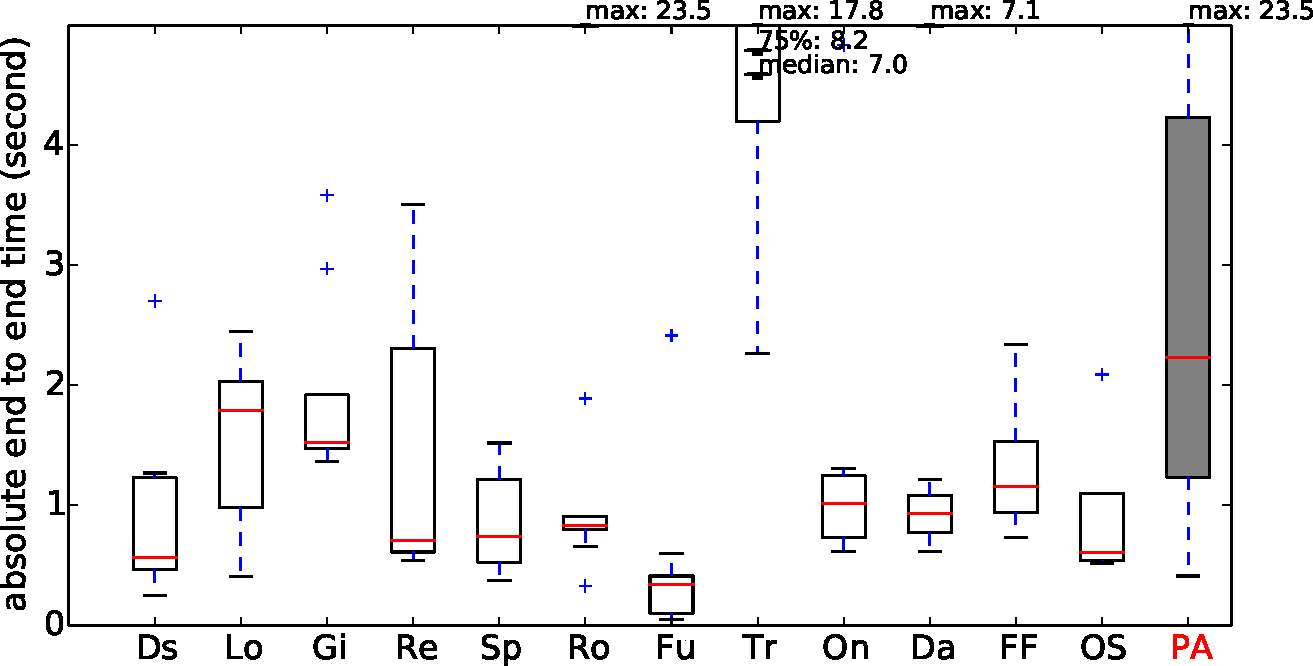
\includegraphics[height=1.75in, width=3.5in]{hownotto/EndToEnd}
\caption{End-to-end page loading time
}
\label{fig:eoeFig}
{\footnotesize Measured for top 10 time-consuming pages per application. Box: 25 to 75 percentile; Red line: median; PA: problematic actions from all 12 applications (see Section~\ref{sec:meth_profile}).\par}
\end{figure}


\begin{figure}
\centering
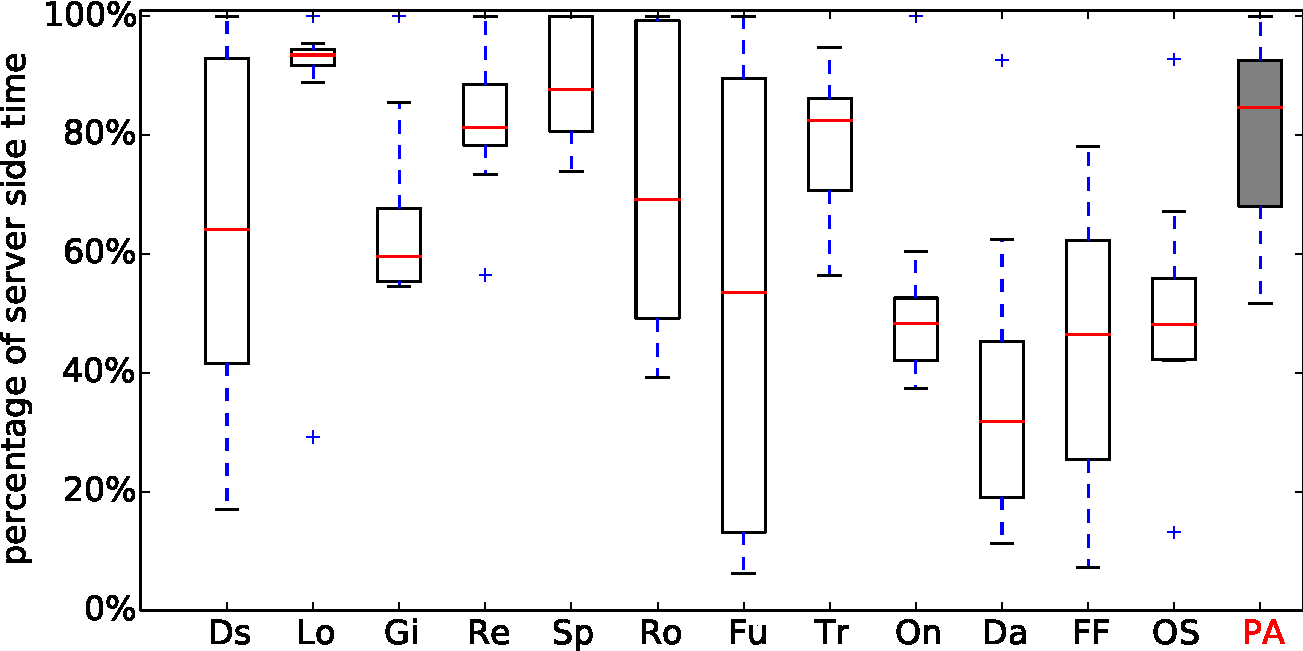
\includegraphics[height=1.75in, width=3in]{hownotto/Percentage}
\caption{Percentage of server time among end-to-end time}
{\footnotesize Measured for top 10 most time-consuming pages per application.
Red line: median; PA: problematic actions from all 12 applications (see Section~\ref{sec:meth_profile})}
\vspace{-0.2in}
\label{percentageFig}
\end{figure}

\begin{comment}
\begin{figure}
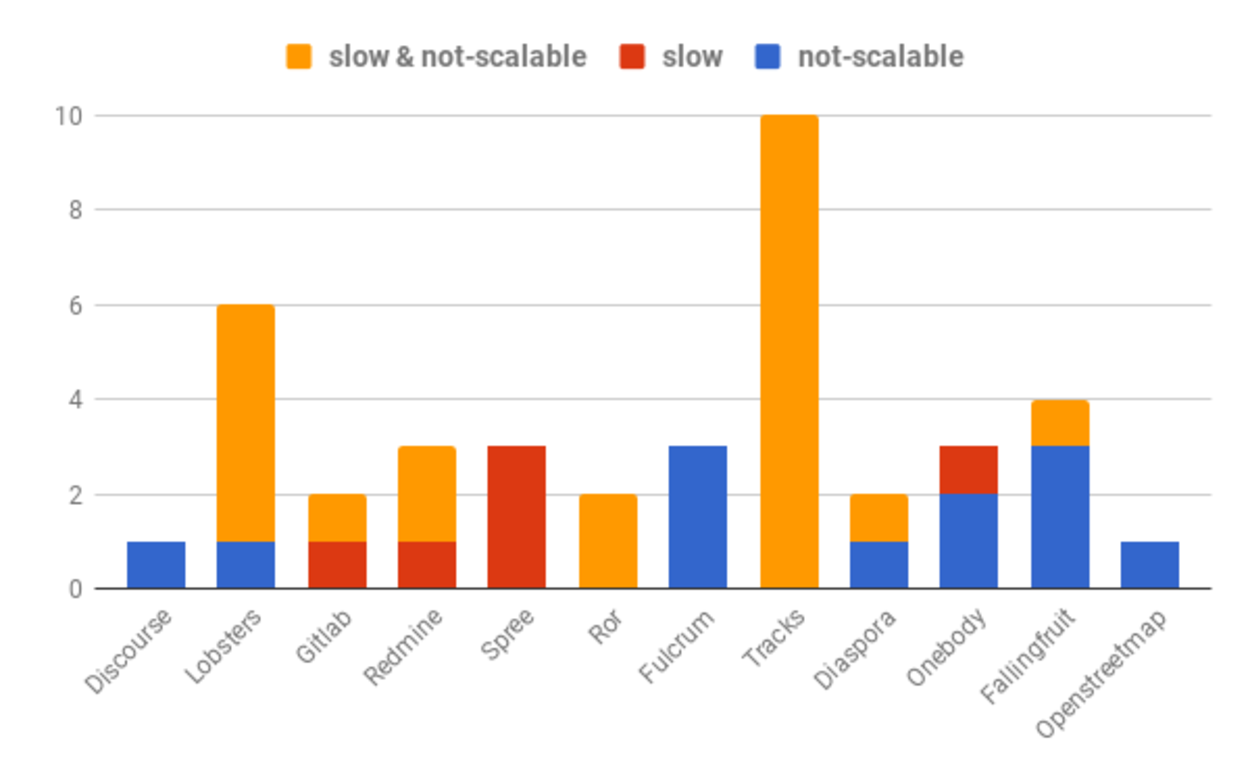
\includegraphics[height=2.2in, width=3.5in]{hownotto/probAct}
\caption{Number of problematic actions}
\label{probAct}
\end{figure}
\end{comment}
\paragraph{\bf{End-to-end loading time}} 
We identify the 10 pages with the most loading time for every application under the 20,000-record database configuration and plot their average end-to-end page loading time in
Figure~\ref{fig:eoeFig}. 11 out of 12 applications have pages whose average end-to-end loading time (i.e., from browser sending the URL request to page finishing loading) exceeds 2 seconds; 6 out of 12 applications have pages that take more than 3 seconds to load. \textit{Tracks} performs the worst: all of its top 10 most time-consuming pages take more than 2 seconds to load. 
%\shan{75\% of top 10 actions?} 
Note that, our workload is 
{\it smaller} or, for some applications, {\it much smaller} than today's real-world workload. Considering how the real-world workload's size will continue growing,
these results indicate that performance problems are prevalent and critical for deployed Rails applications.

\vspace{-0.08in} 
\paragraph{\bf{Server vs. client}}
We break down the end-to-end loading time of the top 10 pages in each 
application into server time (i.e., time for executing controller action, including view rendering and data access, on Rails server), 
client time (i.e., time for loading the DOM in the browser), and network time (i.e., time for data transfer between server and browser).  %\cong{We need to say what's the network latency. Maybe what browser client side uses also matters?} 
As shown in Figure~\ref{percentageFig}, server time contributes to at least 40\% of the end-to-end-latency for more than half of the top 10 pages in all but 1 application.\footnote{Part of the server time could overlap with the client time or the network time. However, our measurement shows that the overlap is negligible.}
Furthermore, over $50\%$ of problematic pages spend more than 80\% of the loading time on Rails server, as shown by the rightmost bar (labeled {\bf PA}) in Figure~\ref{percentageFig}.
%Furthermore, inefficiency in server computation could also affect network latency, as we will see later.
%Our profiling also indicates that server time scales much worse than client time xxx.
This result further motivates us to study the performance problems on the server side of ORM applications.
\vspace{-0.08in} 
\paragraph{\bf{Problematic server actions}}
Table~\ref{tab:probAct} shows the number of problematic actions for each application identified using
the methodology discussed in Section~\ref{sec:meth_profile}. In total, there are \numpactions problematic actions identified from the top 10 most time-consuming actions of every application. Among them, 34 have scalability problems and 28 take more than 1 second of server time. Half of the pages that correspond to these 40 problematic actions take more than 2 seconds to load, as shown in the rightmost bar (labeled {\bf PA}) in Figure~\ref{fig:eoeFig}.
In addition, we find 64 performance issues in these 40 problematic actions, and we will discuss them in detail in Section~\ref{sec:causes}.
%Server time contributes to more than half of the end-to-end time of all the problematic actions (right-most bar in Figure \ref{probAct}). \alvin{didn't we already discuss this in the last paragraph?} 
%\shan{how many have $>1$ second time?}\shan{Hmm, the figure seems to show much fewer number of actions with scalability problems}.

\begin{table}
\centering
\footnotesize
\caption{Number of problematic actions in each application}
\begin{tabular}{@{\hspace{0.1in}}l@{\hspace{0.1in}}l@{\hspace{0.1in}}l@{\hspace{0.1in}}l@{\hspace{0.1in}}l@{\hspace{0.1in}}l@{\hspace{0.1in}}l@{\hspace{0.1in}}l@{\hspace{0.1in}}l@{\hspace{0.1in}}l@{\hspace{0.1in}}l@{\hspace{0.1in}}l@{\hspace{0.1in}}l@{\hspace{0.1in}}}
\toprule
App & Ds & Lo & Gi & Re & Sp & Ro & Fu & Tr & Da & On & FF & OS  \\
\midrule
slow & 0 & 0 & 1 & 1 & 3 & 0 & 0 & 0 & 0 & 1 & 0 & 0 \\
not-scalable & 1 & 1 & 0 & 0 & 0 & 0 & 2 & 0 & 1 & 2 & 3 & 1 \\
slow \& not-scalable & 0 & 5 & 1 & 2 & 0 & 2 & 1 & 10 & 1 & 0 & 1 & 0\\
 \bottomrule
\end{tabular}
\label{tab:probAct}
\vspace{-0.25in}
\end{table}


\section{Causes of Inefficiencies}
\label{sec:causes}


After studying the 64 performance issues in the \numpactions problematic actions and the \numissues issues reported in the applications' bug-tracking systems, we categorize the inefficiency causes into three categories: ORM API misuses, database design, and application design. In the following we discuss these causes and how developers have addressed them. We believe these causes apply to applications built using other ORM frameworks as well, as we will discuss in Section~\ref{sec:dis}. 
%The performance causes that we have observed from performance issue tracking systems and performance action profiling are largely consistent. Also, the way how developers fix the performance issues from issue tracking systems are consistent with what we have done for the profiling issues. Consequently, we will discuss them together below. 

%\shan{are these ALL inefficiency problems or ALL inefficient-data-processing problems?}\shan{What about rendering problems; rendering template optimization?}

\begin{comment}

\end{}

\newcolumntype{g}{>{\columncolor{Gray}}r}
\begin{table*}[]
\centering
\small
\caption{Causes for problematic actions and performance issues}
\label{tab:freq}
\begin{tabular}{@{}llggggggggggggg@{}}
\toprule

\rowcolor{white}
 & Causes &Ds & Lo & Gi & Re & Sp & Ro & Fu & Tr & Da & On & FF & OS& SUM  \\
 \midrule
\rowcolor{white}
 & Inefficient  & { 0} & {0} & 0 & 0 & 0 & 1 & 0 & 1 & 2 & 2 & 2 & 0 & 8 \\
\cmidrule{3-15}
 & computation & 0 & 0 & 3 & 6 & 5 & 0 & 0 & 2 & 2 & 0 & 0 & 0 & 18 \\ 
\cmidrule{2-15}

\rowcolor{white}
 & Unnecessary  & 0 & 3 & 0 & 0 & 0 & 0 & 0 & 0 & 0 & 0 & 2 & 0 & 5 \\
\cmidrule{3-15}
API & Computation & 1 & 0 & 3 & 4 & 4 & 1 & 0 & 1 & 2 & 1 & 0 & 0 & 17 \\
\cmidrule{2-15}

\rowcolor{white}
Usage & Inefficient  & 0 & 1 & 0 & 0 & 3 & 2 & 0 & 2 & 2 & 3 & 0 & 1 & 14 \\
\cmidrule{3-15}
 &data accessing  & 3 & 0 & 4 & 5 & 10 & 0 & 0 & 2 & 0 & 2 & 0 & 0 & 26 \\
\cmidrule{2-15}
\rowcolor{white}
 & Unnecessary & 0 & 0 & 1 & 0 & 0 & 0 & 0 & 0 & 0 & 0 & 0 & 0 & 1 \\
\cmidrule{3-15}
 & data loading  & 2 & 0 & 3 & 1 & 2 & 0 & 0 & 0 & 0 & 0 & 0 & 0 & 8 \\
\cmidrule{2-15}
 \rowcolor{white}
 & Inefficient Rendering & 0 & 3 & 1 & 0 & 0 & 0 & 0 & 1 & 0 & 0 & 0 & 0 & 5 \\
\midrule


\rowcolor{white}
 & Missing  & 0 & 0 & 0 & 1 & 0 & 0 & 0 & 0 & 0 & 0 & 1 & 1 & 3 \\
\cmidrule{3-15}
 & Fields & 0 & 2 & 0 & 0 & 2 & 0 & 0 & 0 & 0 & 0 & 1 & 0 & 5 \\
\cmidrule{2-15}

\rowcolor{white}
Database& Missing  & 0 & 0 & 0 & 0 & 0 & 0 & 0 & 1 & 0 & 0 & 0 & 0 & 1 \\
\cmidrule{3-15}
 Design& association & 0 & 1 & 0 & 0 & 1 & 0 & 0 & 0 & 1 & 0 & 0 & 0 & 3 \\
 
\cmidrule{2-15}

\rowcolor{white}
   & Missing  & 0 & 1 & 0 & 0 & 0 & 0 & 0 & 0 & 0 & 0 & 2 & 0 & 3 \\
\cmidrule{3-15}
 & index & 3 & 1 & 4 & 6 & 3 & 0 & 0 & 3 & 5 & 1 & 1 & 3 & 30 \\
\midrule

\rowcolor{white}
& Unworthy  & 1 & 0 & 0 & 2 & 0 & 2 & 6 & 10 & 0 & 1 & 0 & 0 & 22 \\
\cmidrule{3-15}
App & content & 5 & 1 & 1 & 0 & 0 & 1 & 0 & 3 & 1 & 0 & 0 & 2 & 14 \\
 \cmidrule{2-15}
\rowcolor{white}
Design & Unworthy  & 0 & 2 & 0 & 0 & 0 & 0 & 0 & 0 & 0 & 0 & 0 & 0 & 2 \\
 \cmidrule{3-15}
 & features & 3 & 2 & 4 & 0 & 1 & 0 & 2 & 1 & 2 & 1 & 1 & 2 & 19 \\
 \midrule
 

\rowcolor{white}
SUM &  & 18 & 17 & 24 & 25 & 31 & 7 & 8 & 27 & 17 & 11 & 10 & 9 & 204\\
\bottomrule
\end{tabular}
\\
\footnotesize{data with white background is for problematic actions from 12 representative applications\\ data with gray background is for performance issues from 12 bug-tracking systems}
\end{table*}
\end{comment}
\definecolor{LightCyan}{rgb}{0.88,1,1}
%\definecolor{Gray}{gray}{0.9}
\definecolor{Gray}{rgb}{0.6,0.6,0.6}
\newcolumntype{g}{>{\columncolor{Gray}}r}
\begin{table}[]
\centering
\small
\caption{Inefficiency causes across 12 applications}
\label{tab:freq}
\begin{tabular}{@{\hspace{0.1in}}c@{\hspace{0.1in}}g@{\hspace{0.1in}}g@{\hspace{0.1in}}g@{\hspace{0.1in}}g@{\hspace{0.1in}}g@{\hspace{0.1in}}g@{\hspace{0.1in}}g@{\hspace{0.1in}}g@{\hspace{0.1in}}g@{\hspace{0.1in}}g@{\hspace{0.1in}}g@{\hspace{0.1in}}g@{\hspace{0.1in}}g@{\hspace{0.1in}}}
\toprule

\rowcolor{white}
   &Ds & Lo & Gi & Re & Sp & Ro & Fu & Tr & Da & On & FF & OS& Sum  \\
 \midrule
\rowcolor{white}
\multicolumn{13}{c}{\bf ORM API Misuse}\\
\midrule
\rowcolor{white}
\multirow{ 2}{*}{IC}  & { 0} & {0} & 0 & 0 & 0 & 1 & 0 & 1 & 2 & 2 & 2 & 0 & 8 \\
\cmidrule{2-14}

  & 0 & 0 & 3 & 6 & 5 & 0 & 0 & 2 & 2 & 0 & 0 & 0 & 18 \\ 
\cmidrule{1-14}

\rowcolor{white}
\multirow{ 2}{*}{UC}   & 0 & 3 & 0 & 0 & 0 & 0 & 0 & 0 & 0 & 0 & 2 & 0 & 5 \\
\cmidrule{2-14}
  & 1 & 0 & 3 & 4 & 4 & 1 & 0 & 1 & 2 & 1 & 0 & 0 & 17 \\
\cmidrule{1-14}

\rowcolor{white}
 \multirow{ 2}{*}{ID}   & 0 & 1 & 0 & 0 & 3 & 2 & 0 & 3 & 2 & 3 & 0 & 1 & 15 \\
\cmidrule{2-14}
   & 3 & 1 & 4 & 5 & 11 & 0 & 0 & 2 & 1 & 2 & 0 & 0 & 29 \\
\cmidrule{1-14}
\rowcolor{white}
  \multirow{ 2}{*}{UD}  & 0 & 0 & 1 & 0 & 0 & 0 & 0 & 0 & 0 & 0 & 0 & 0 & 1 \\
\cmidrule{2-14}
    & 2 & 0 & 3 & 1 & 2 & 0 & 0 & 0 & 0 & 0 & 0 & 0 & 8 \\
\cmidrule{1-14}
 \rowcolor{white}
   IR & 0 & 3 & 1 & 0 & 0 & 0 & 0 & 1 & 0 & 0 & 0 & 0 & 5 \\
\midrule

\rowcolor{white}
\multicolumn{13}{c}{\bf Database Design Problems}\\
\midrule
\rowcolor{white}
  \multirow{ 2}{*}{MF}   & 0 & 0 & 0 & 1 & 0 & 0 & 0 & 0 & 0 & 0 & 1 & 1 & 3 \\
\cmidrule{2-14}
   & 0 & 2 & 0 & 0 & 2 & 0 & 0 & 0 & 0 & 0 & 1 & 0 & 5 \\
\cmidrule{1-14}
\rowcolor{white}
   \multirow{ 2}{*}{MI}   & 0 & 1 & 0 & 0 & 0 & 0 & 0 & 0 & 0 & 0 & 2 & 0 & 3 \\
\cmidrule{2-14}
   & 3 & 1 & 4 & 6 & 3 & 0 & 0 & 3 & 5 & 1 & 1 & 3 & 30 \\
\midrule
\rowcolor{white}
\multicolumn{13}{c}{\bf Application Design Tradeoffs}\\
\midrule
\rowcolor{white}
 \multirow{ 2}{*}{DT}   & 1 & 0 & 0 & 2 & 0 & 2 & 6 & 10 & 0 & 1 & 0 & 0 & 22 \\
\cmidrule{2-14}
  & 5 & 1 & 1 & 0 & 0 & 1 & 0 & 3 & 1 & 0 & 0 & 2 & 14 \\
 \cmidrule{1-14}
\rowcolor{white}
  \multirow{ 2}{*}{FT}   & 0 & 2 & 0 & 0 & 0 & 0 & 0 & 0 & 0 & 0 & 0 & 0 & 2 \\
 \cmidrule{2-14}
  & 3 & 2 & 4 & 0 & 1 & 0 & 2 & 1 & 2 & 1 & 1 & 2 & 19 \\
 \midrule
 

\rowcolor{white}
Sum  & 18 & 17 & 24 & 25 & 31 & 7 & 8 & 27 & 17 & 11 & 10 & 9 & 204\\
\bottomrule
\end{tabular}
\\
\footnotesize{Data with white background shows 64 issues from 40 problematic actions\\ Data with gray background shows 140 issues from 12 bug-tracking systems\\
\begin{tabular}{rlrl}
IC:& Inefficient Computation & MF:& Missing Fields \\
UC:& Unnecessary Computation & MI:& Missing Indexes \\
ID:& Inefficient Data Accessing & DT:& Content Display Trade-offs\\
UD:& Unnecessary Data Retrieval & FT:& Functionality Trade-offs\\
IR:& Inefficient Rendering & \\

\end{tabular}
}

\vspace{-0.10in}
\end{table}

\subsection{ORM API Misuses} 
\label{causes:api}

About half of the performance issues that we studied suffer from API misuses. In these cases, performance can be improved by changing how the Rails APIs are used without modifying program semantics or database design. While some of these misuses appear simple, making the correct decision requires deep expertise in the implementation of the ORM APIs and query processing.

%\shan{TODO: 1.discuss scalability problems 2. add some profiling examples, instead of all examples from bug-tracking system?}
\vspace{-0.1in}

\subsubsection{Inefficient Computation (IC)}
\label{sec:inefficomp}

In these cases, the poorly performing code conducts useful computation but inefficiently.
Such cases comprise more than 10\% of the performance issues in both bug reports and problematic actions. 
\vspace{-0.18in} 
\paragraph{\bf{Inefficient queries}}
The same operation on persistent data can be implemented via different ORM calls. However, the performance of the generated queries can be drastically different. This problem has not been well studied before for ORM applications.
%A functionality can be accomplished by different database queries and developers unfortunately use a more expensive query. This problem is widespread and is difficult to avoid for developers who cannot easily track which queries are transparently generated by ORM or whether the queries are efficient. Unfortunately, there was no automated solution yet.

Figure~\ref{fig:spreeAnyVsExists} shows two ways that an online shopping system checks if there are product \texttt{variants} whose inventory are not tracked.
%(i.e., \texttt{track\_inventory} field is \texttt{false}).
The Ruby code differs only in the use of 
\texttt{any?} vs \texttt{exists?}. However, the performance of the generated queries differs substantially:
the generated query in Figure~\ref{fig:spreeAny} scans all records in the \texttt{variants} table to compute the count if no index exists, but that in Figure~\ref{fig:spreeExists} only needs to scan and locate the first 
\texttt{variant} record where the predicate evaluates to true. \texttt{Spree} developers discovered and fixed this problem in 
\texttt{Spree-6720}.\footnote{We use \texttt{A-n} to denote report number {\tt n} in application {\tt A}'s bug-tracking system.}
% we mention that this is widespread in 2 sentences
%This problem is widespread as we find that it contributes to 3 problematic actions in 2 applications. 
Our profiling finds similar problems. For example, simply replacing \texttt{any?} with \texttt{exists?} in a problematic action of \texttt{OneBody} improves server time by 1.7$\times$. 
%\alvin{how about say how much improvement for the spree code shown rather than citing another example?}
Our static checker that will be discussed in Section~\ref{sec:dis} finds that this is a common problem as it appears in the latest versions of 9 out of 12 applications under study.

\begin{comment}
\begin{figure}[h]
  \centering
  \begin{subfigure}[t]{0.5\textwidth}
  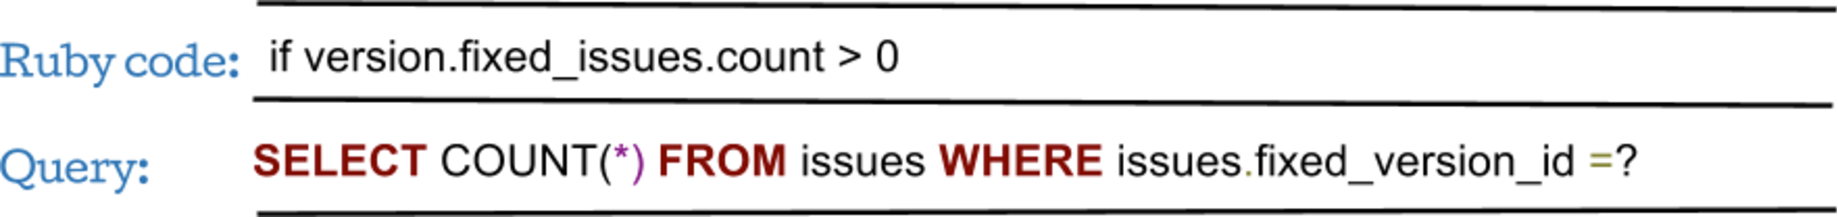
\includegraphics[width=0.95\columnwidth]{figs/countstar}
  %\caption{Inefficient API}
  \label{InefficientAPI}
  \end{subfigure}
  
    \centering
  \begin{subfigure}[t]{0.5\textwidth}
  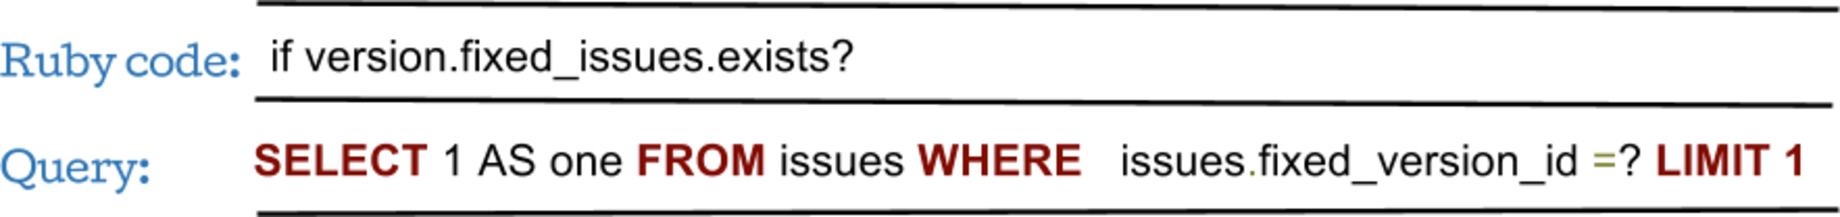
\includegraphics[width=0.95\columnwidth]{figs/exist}
  	%\caption{Efficient API}
  \label{efficientAPI}
  \end{subfigure}

  \caption{Inefficient query due to improper APIs in Redmine}
  \label{API}
\end{figure}
\end{comment}

\begin{comment}
\begin{figure}[h]
  \centering
  \begin{subfigure}[t]{0.5\textwidth}
  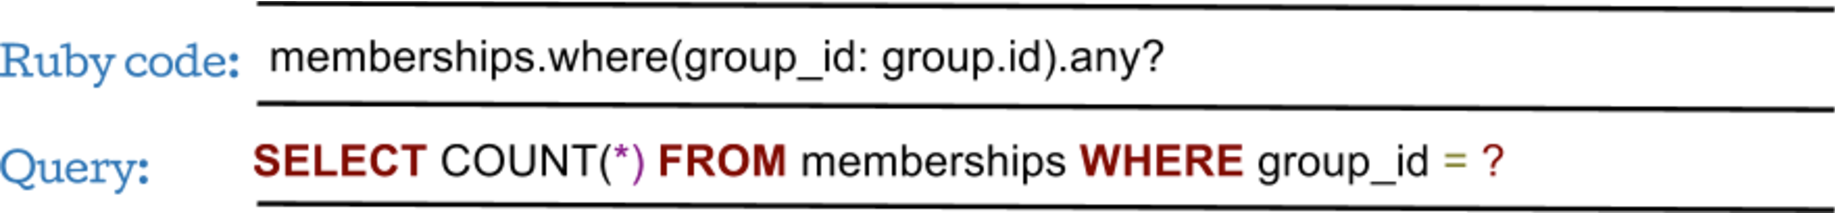
\includegraphics[width=0.95\columnwidth]{figs/any}
  \caption{Inefficient API}
  
  \label{fig:any}
  \end{subfigure}
  
    \centering
  \begin{subfigure}[t]{0.5\textwidth}
  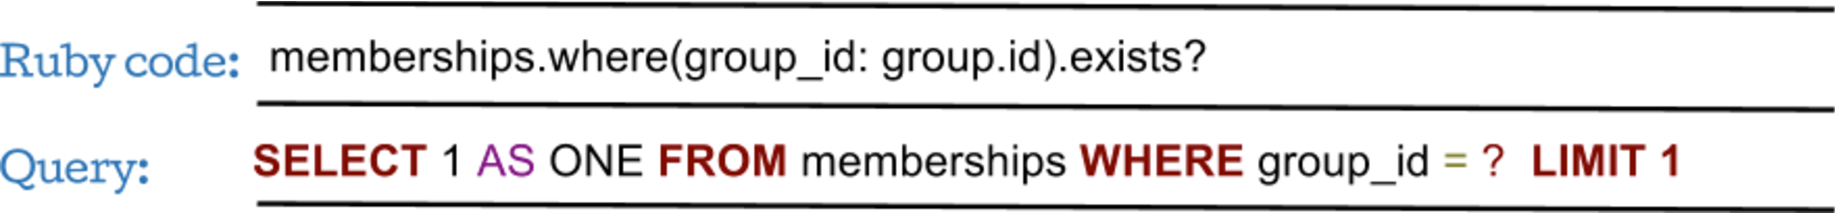
\includegraphics[width=0.95\columnwidth]{figs/exists}
  	\caption{Efficient API}
  \label{fig:exists}
  \end{subfigure}

  \caption{Inefficient query due to improper APIs in Onebody}
  \label{fig:anyVsExists}
\end{figure}
\end{comment}

\begin{figure}
  \vspace{-0.05in}
  \centering
  \begin{subfigure}[t]{60mm}

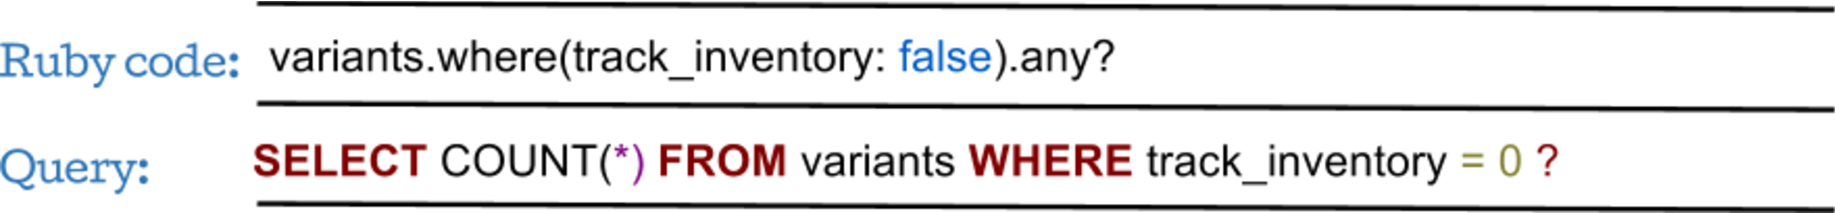
\includegraphics[width=0.95\columnwidth]{figs/spreeAny}
  \caption{Inefficient}
  
  \label{fig:spreeAny}
  \end{subfigure}
  
    \centering
  \begin{subfigure}[t]{60mm}
  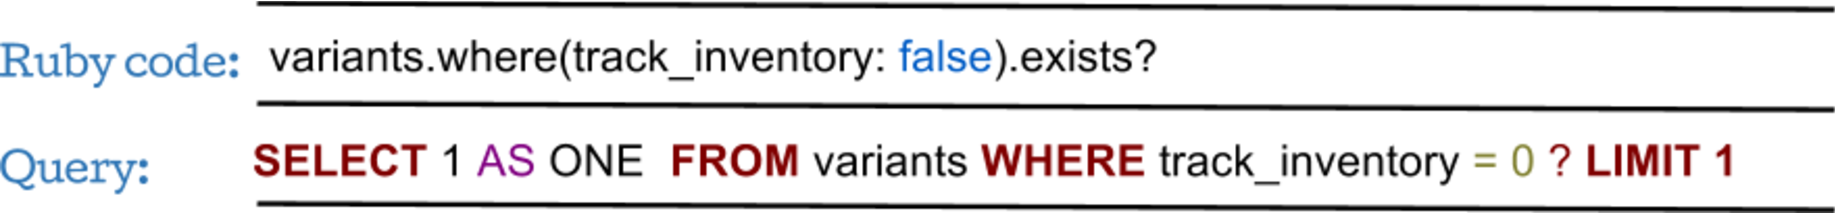
\includegraphics[width=0.95\columnwidth]{figs/spreeExists}
  	\caption{Efficient}
    
  \label{fig:spreeExists}
  \end{subfigure}

  \caption{Different APIs cause huge performance difference}
  %Inefficient query due to improper APIs in Spree}
  \label{fig:spreeAnyVsExists}
  \vspace{-0.25in}
\end{figure}

Another common problem is developers using API calls that generate queries with unnecessary ordering of the results. For example, Ror, Diaspora, and Spree developers use \texttt{Object.}\texttt{where(c).first} to get an object satisfying predicate \texttt{c} instead of \texttt{Object.find\_by(c)}, not realizing that the former API orders {\tt Object}s by primary key after evaluating predicate {\tt c}. 
As a fix, both Gitlab and Tracks developers explicitly add \texttt{except(:order)} in 
the patches to eliminate unnecessary ordering in the queries, further showing how simple changes can lead to drastic performance difference.

\vspace{-0.08in} 
\paragraph{\bf{Moving computation to the DBMS}} %Should Be a Query}}
As the ORM framework hides the details of query generation, developers often write code that results in multiple queries being generated. Doing so incurs extra network round-trips, or running computation on the server rather than the DBMS, which leads to performance inefficiencies.

%
%A functionality is faster to accomplish by one query. Unfortunately, the developers use either (1) multiple queries or (2) one query together with in-memory computation. Either way, inefficiency is incurred by extra query and/or data round-trips. Although the general problem of pushing application computation down to database has been tackled by previous work \cite{cheung:pldi13} using program synthesis, our study finds that many such problems in Rails are caused by simple API misuses and hence could benefit from a new tool that is less general but much simpler.
%
%There are many cases that only involve one expression and simple API misuses.
For example, the patch of \texttt{Spree-6720} replaces
\texttt{if(exist?)} \texttt{find; else create} with 
\texttt{find\_or\_create\_by}, where the latter combines two queries that are issued by \texttt{exist}
and \texttt{find}/\texttt{create} into one.
The patch of \texttt{Spree-6950} replaces
\texttt{pluck(:total).sum} with \texttt{sum(:total)}. The former uses \texttt{pluck} to issue
a query to load the \texttt{total} column of all corresponding records and then
computes the sum in memory, while the latter uses \texttt{sum} to issue a 
query that directly performs the sum in the DBMS without returning actual records to the server.
The patch of {\tt Gitlab-3325} replaces \texttt{pluck(:id)+pluck(:id)}, which replaces two queries and an in-memory union via {\tt +} with one SQL \texttt{UNION} query, in effect 
moving the computation to the DBMS.
%conducts the summation in database and hence saves data loading time. 
%This was from the bug-tracking system of Gitlab, and we also see similar cases in Spree.
Such API misuses are very common and occur in many applications as we 
will discuss in Section~\ref{sec:dis}. 



%For example, xxx developers use \texttt{array.count} instead of \texttt{array.size} to get the size of an array. When \texttt{array} is already loaded in memory, the former issues a query to do the counting in database, while the latter conducts in-memory size computation and hence is much more efficient.

There are also more complicated cases where a loop implemented in Ruby can be completely pushed
down to DBMS,  which has been addressed in
previous work using program synthesis~\cite{cheung:pldi13}.

%where the Rails program iterate through a container
%filled with data previously loaded from database 
%As another example, it could cause many rows to be loaded to memory for selection that should have been done in database.
%An example of row-wise unnecessary data retrieval is shown in Fig \ref{rowwise}. Ruby code in Fig \ref{posts} from \texttt{Spree-6903} first retrieves all posts of ``StatusMessage'' type, and then through \texttt{tagged\_with}, only posts with specified \texttt{tagged\_name} will be rendered. Other posts are useless. A better way to avoid unnecessary data is to issue another query which will only retrieve the posts with specified \texttt{tag\_name} as shown in Fig \ref{taggings}. This simple change would save the corresponding action in software xxx xx based on our profiling.

%Redundant row retrieval problem has not been studied by previous work.
%\shan{is this right?} 

%Furthermore, it is difficult for developers to avoid this problem. In fact, the more efficient code shown in Figure \ref{rowwise} may actually be considered as ``message chain'' code smell. It is difficult for developers to realize that such smell code is actually much more efficient. Future work should build xx to automatically detect and fix this xxx.

%\begin{figure}[h]
%  \centering
%  \begin{subfigure}[t]{0.5\textwidth}
%  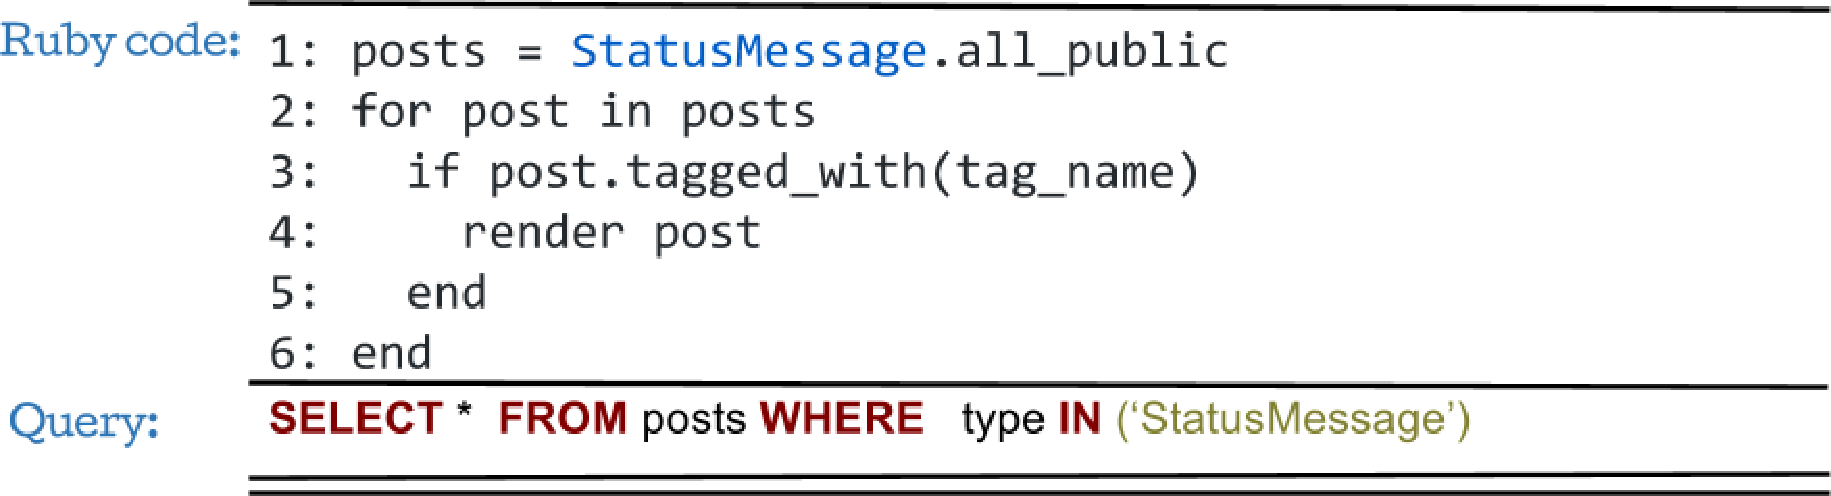
\includegraphics[width=1\columnwidth]{figs/posts}
%  \caption{Unoptimized} 
%  \label{posts}
%  \end{subfigure} 
%    \centering
%  \begin{subfigure}[t]{0.5\textwidth}
%  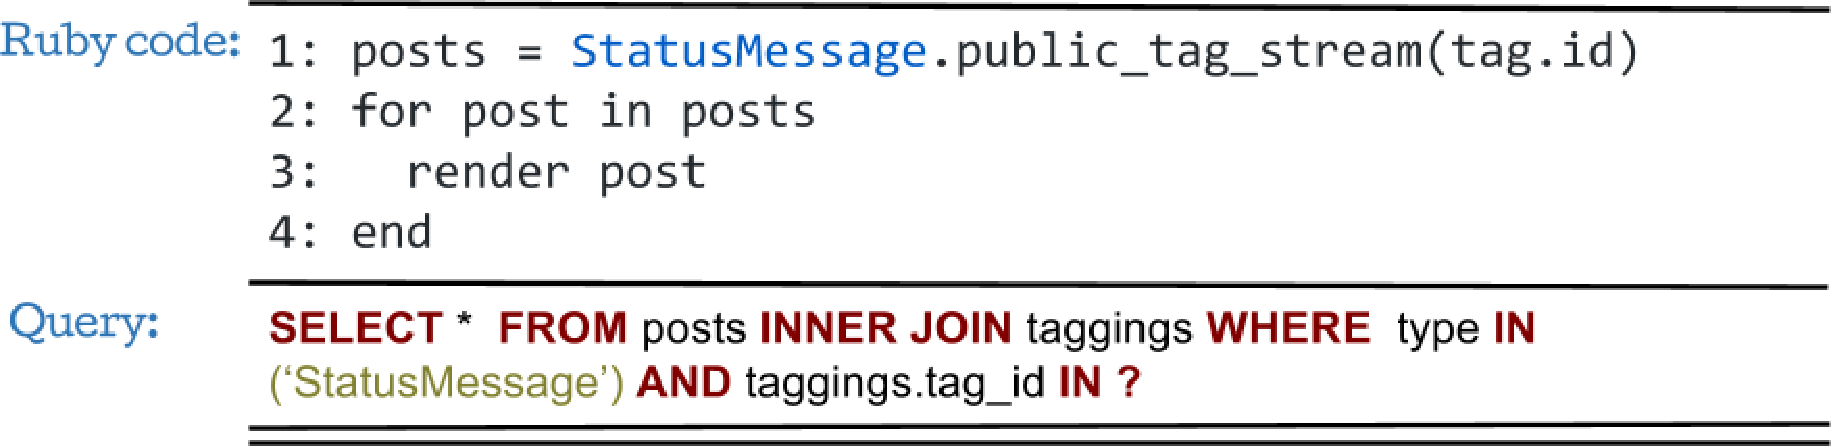
\includegraphics[width=1\columnwidth]{figs/taggings}
%  	\caption{Optimized}
%  \label{taggings}
%  \end{subfigure}
%  \caption{Unnecessary row-data retrieval in xxx}
%  \label{rowwise}
%\end{figure}
\vspace{-0.08in} 
\paragraph{\bf{Moving computation to the server}} %Should Not be a Query}} 
Interestingly, there are cases where the computation should be moved to the server from the DBMS. %a functionality is faster to do by in-memory computation instead of a database query. 
As far as we know, this issue has not been studied before. 
%and is naturally out of the scope of database optimization. 

%
For example, in the patch of \texttt{Spree-6819}, developers replace 
\texttt{Objects.count} with \texttt{Objects.size} in 17 different locations, as
\texttt{count} always issues a \texttt{COUNT} query while \texttt{size} counts the 
\texttt{Objects} in memory
if they have already been retrieved from the database by earlier computation.
%and issues a count SQL query otherwise. 
%However, as all instances are in views (not controllers) or in utility functions, merging them with other code such that the appropriate call can be made will break code modularity, making it a difficult choice for developers.
%Consequently, code modularity concerns prevent them from being merged with other queries. 
Such issues are also reported in {\tt Gitlab-17960}.

\vspace{-0.08in} 
\paragraph{\bf{Summary}} Rails, like other ORM frameworks, lets developers implement a given functionality in various ways.
%With ORM framework, a functionality can often be implemented by different combinations of queries and in-memory computation. 
Unfortunately, developers often struggle at 
picking the most efficient option. The deceptive names of many 
Rails APIs like \texttt{count} and \texttt{size} make this even more challenging. Yet, we believe many cases can be fixed using simple static analyzers, as we will discuss in Section~\ref{sec:dis}.
%Meanwhile, many inefficient API patterns are simple and repeatedly appear in different applications. It is both feasible and very helpful to build static analysis tools to automatically identify and/or fix inefficient API uses. More complicated cases would benefit from general query synthesis techniques \cite{cheung:pldi13}.

\begin{figure}
  \centering
  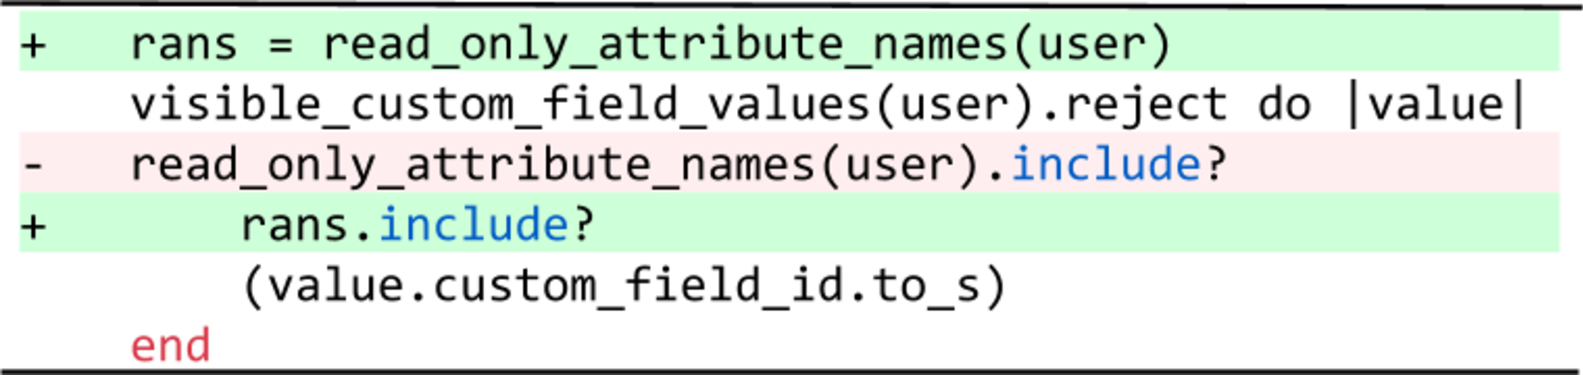
\includegraphics[width=0.7\columnwidth]{hownotto/redCom}
  \caption{A loop-invariant query in Redmine}
  \label{fig:redCom}
\end{figure}

\subsubsection{Unnecessary Computation (UC)} 
\label{sec:uncomp}
More than 10\% of the performance issues are caused by (mis)using ORM APIs that lead to unnecessary queries being issued. This type of problems has not been studied before.
%The poorly performing code issues unnecessary queries. It happens for about 10\% of studied performance issues, and also causes problematic actions in the latest versions of multiple applications.
\vspace{-0.08in} 
\paragraph{\bf{Loop-invariant queries}}
Sometimes, queries are repeatedly issued to load the {\it same} database contents and hence are unnecessary. 
%In traditional programs, these problems can be solved by classic optimization techniques, which we will discuss below. Unfortunately, problems here require the optimizer to understand both ORM/query semantics and Ruby application semantics, and have not been tackled by previous research.
%
%Sometimes, a query is repeatedly issued in a loop to return the same content --- it could be optimized by \textit{loop-invariant code motion} if the optimizer understands not only Ruby logic but also ORM and queries.
For instance, Figure~\ref{fig:redCom} shows the patch from \texttt{redmine-23334}.
This code iterates through every custom field 
\texttt{value} %that is visible to the \texttt{user} 
and retains only those that 
\texttt{user} has write access to.
%, \texttt{reject}ing the read-only ones. 
To conduct this access-permission checking, in every iteration, \texttt{read\_only\_attribute\_}
\texttt{names(user)} issues a query to get the names of all read-only fields of \texttt{user}, as shown by the red highlighted line
in the figure. Then, if
\texttt{value} belongs to this read-only set, it will be excluded from the return set of this function (i.e., the \texttt{reject} at the beginning of the loop takes effect). Here, the \texttt{read\_only\_attribute\_names(user)} query 
returns exactly the same result during every iteration of the loop and causes
unnecessary slowdowns. 
%\alvin{I am confused. What is the original code? The red line? Why are we showing the a patch but not discussing it. Add line numbers?}
As shown by the green lines in figure, Redmine developers hoist loop invariant \texttt{read\_only\_attribute\_names(user)} outside the loop and achieve more than 20$\times$ speedup for the corresponding function for their workload.
%, shortening its time from 1.03 second to 0.05 second with 1000 issues.
Similar issues also occur in Spree and Discourse.





\vspace{-0.08in} 
\paragraph{\bf{Dead-store queries}}
In such cases, queries are repeatedly issued to load {\it different} database contents into the same memory object while the object has not been used between the reloads.
%without using the object in between --- it could be optimized by
%\textit{dead-store elimination} if the optimizer understands not only Ruby but also ORM and queries. 
 For example, in Spree, every shopping transaction has a corresponding
 {\tt order} record in the {\tt orders} table. This table has a
 {\tt has\_many} association relationship with the 
 {\tt line\_items} table, meaning that every order  contains
 multiple lines of items. Whenever the user updates his/her shopping
 cart, the {\tt line\_items} table would change, at which point the old version of Spree always uses an {\tt order.reload} to make 
 sure that the in-memory copy of {\tt order} and its associated 
 {\tt line\_item}s are up-to-date. Later on, developers realize that
 this repeated reload is unnecessary, because the content of 
 {\tt order} is not used by the program until check out.
 Consequently, in {\tt Spree-6379}, developers remove many 
 {\tt order.reload} from model classes, and instead add it in a few places in the {\tt before\_payment} action of the
 {\tt checkout} controller, where the {\tt order} object is to be used.
%\alvin{how does this justify issuing repeated reads?} 


%original listing
\begin{comment}

\begin{lstlisting}[language=Ruby, numbers=left, firstnumber=1, numberstyle=\tiny\color{gray}, caption={redundant computation from redmine~\cite{redmine}.},label={redundantComputation}, numbers = none]
@\lstlabel{redundantComputation}@ visible_custom_field_values(user).reject do |value| 
 read_only_attribute_names(user).include?(value.custom_field_id.to_s) 
@\lstlabel{end}@ end
\end{lstlisting}

\begin{lstlisting}[language=Ruby, numbers=left, firstnumber=1, numberstyle=\tiny\color{gray}, caption={remove redundant computation from redmine~\cite{redmine}.},label={removeredundantComputation}, numbers = none]
@\lstlabel{removeredundantComputation}@ 
read_only_attr_names_array = read_only_attribute_names(user)
visible_custom_field_values(user).reject do |value|
  read_only_attr_names_array.include?(value.custom_field_id.to_s)
end
\end{lstlisting}

\end{comment}

\begin{figure}

  \centering
  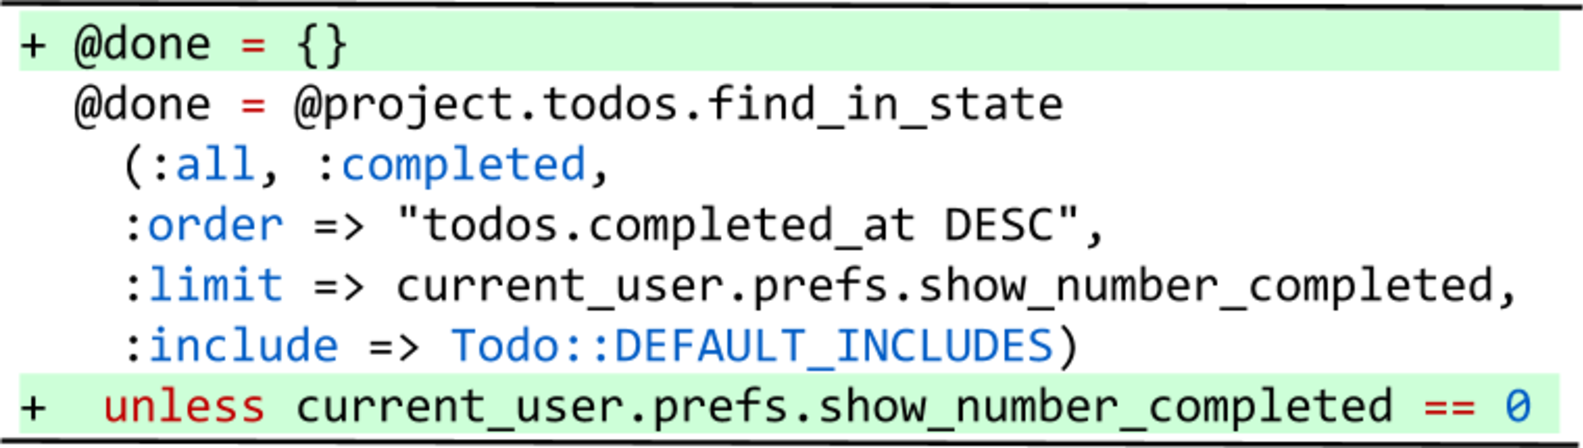
\includegraphics[width=0.7\columnwidth]{hownotto/tracks63}
  \caption{A query with known results in Tracks}
  \label{fig:tracks63}
\end{figure}

\vspace{-0.08in} 
\paragraph{\bf{Queries with known results}}
A number of issues are due to issuing queries whose results are already known, hence incurring unnecessary network round trips and query processing time.
%Occasionally, certain value of a Rails API parameter would cause the corresponding query to return a predictable constant result. If that specific parameter value is common, it is better to issue the query conditionally. This optimization again requires knowledge about both application semantics and ORM/query, and is not handled by existing techniques.
%
An example is in \texttt{Tracks-63}. As shown in Figure~\ref{fig:tracks63},
the code originally issues a query to retrieve up to 
\texttt{show\_number\_completed} number of completed tasks. Clearly, when \texttt{show\_number\_completed} is $0$, the query always returns an empty set due to {\tt limit} being $0$.
Developers later realize
that $0$ is a very common setting for \texttt{show\_number\_completed}. 
%In fact, the corresponding view file \texttt{show.html.erb} has already been designed to render the completed-todo panel only conditionally.
Consequently, they applied the patch shown in Figure \ref{fig:tracks63} to only issue the query when needed. 
%\alvin{say something about how prevalent this is?}

\vspace{-0.08in} 
\paragraph{\bf{Summary}}
While similar issues in general purpose programs can be eliminated using classic compiler optimization techniques (e.g., loop invariant motion, dead-store elimination), doing so for ORM applications is difficult as it involves understanding database queries.
% and performing inter-action data-flow analysis. 
We are unaware of any compilers that perform such transformations.
%Correctly detecting and fixing unnecessary computation discussed above are non-trivial. 
%Furthermore, they often require inter-action data-flow analysis. 
%ORM developers will benefit from techniques that integrate ORM and database knowledge into traditional compiler optimization techniques like loop-invariant code motion, dead-store elimination, and others.

\vspace{-0.08in} 
\subsubsection{Inefficient Data Accessing (ID)} 
\label{sec:iffidata}
Problems under this category suffer from data transfer slow downs, including not batching data transfers (e.g., the well-known ``N+1'' problem) or batching too much data into one transfer.

\vspace{-0.08in} 
\paragraph{\bf{Inefficient lazy loading}}
As discussed in Section~\ref{sec:background}, when a set of objects $O$ in table $T_1$ are requested, objects stored in table $T_2$ associated with $T_1$ and $O$ can be loaded together through eager loading. If lazy loading is chosen instead, 
one query will be issued to load $N$ objects from $T_1$, and then
$N$ separate queries have to be issued to load associations of each such object from $T_2$. This is known as the ``N+1'' query problem. While prior work has studied this problem~\cite{nplusone, cheung:sigmod14:sloth, bullet}, we find it still prevalent: it appears in 15 problematic actions and 9 performance issues in our study. 
%This is a well known problem and can be tackled by research techniques \cite{} and Rails plugins \cite{bullet}.

Figure~\ref{fig:nplusone} shows an example that we find in the latest version of Lobsters, where the deleted code retrieves 50 \texttt{mods} objects. Then, for each \texttt{mod}, a query is issued to retrieve its associated \texttt{story}. Using eager loading in the added line, all 51 queries (and hence 51 network round-trips) will be combined together. In our experiments, the optimization reduces the end-to-end loading time of the corresponding page from 1.10 seconds to 0.34 seconds.

% Bullet is a rails gem, Sloth
%Several previous work can help developers avoid the above lazy loading problems. For example, a Rails plugin, Bullet\cite{bullet}, can warn developers about ``N + 1'' problems and remind them to use eager loading. Sloth \cite{cheung:sigmod14:sloth} will automatically batch queries to avoid N + 1 queries without developers' specifying loading strategies
%\shan{hmm, is this lazy loading or eager loading}.


\begin{figure}
  \centering
  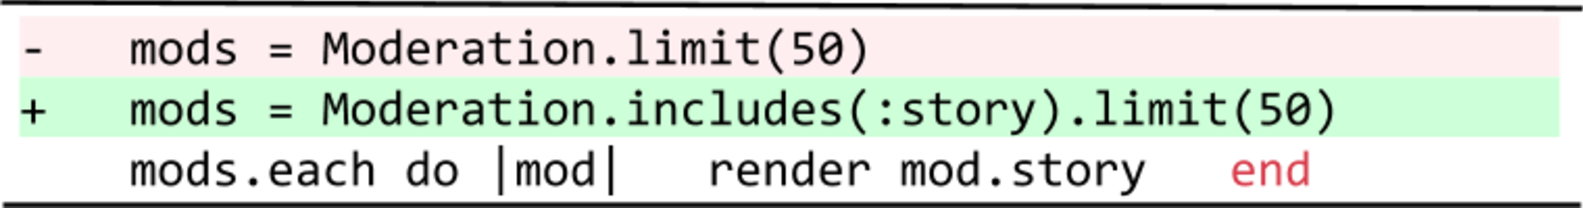
\includegraphics[width=0.7\columnwidth]{hownotto/moderations}
  \caption{Inefficient lazy loading in Lobsters}
  \label{fig:nplusone}
\end{figure}

\begin{comment}
\begin{lstlisting}[language=Ruby, numbers=left, firstnumber=1, numberstyle=\tiny\color{gray}, caption={N + 1 queries from redmine~\cite{redmine}.},label={nplusone}]
mods = Moderation.order("id desc").limit(50)
mods.each do |mod|
  if mod.user
  	puts mod.user.username
  end
end
\end{lstlisting}

\begin{lstlisting}[language=Ruby, numbers=left, firstnumber=1, numberstyle=\tiny\color{gray}, caption={remove N + 1 queries from lobsters~\cite{lobsters}\shan{redmine?}.},label={rmnplusone}, numbers = none]
mods = Moderation.includes(:user).order("id desc").limit(50)
\end{lstlisting}
\end{comment}

\vspace{-0.08in} 
\paragraph{\bf{Inefficient eager loading}}
However, always loading data eagerly can also cause problems. \textcolor{black}{ Specifically, when the associated objects are too large, loading them all at once will create huge memory pressure and even make the application unresponsive.}
In contrast to the ``N+1'' lazy loading problem, there is little support for developers to detect eager loading problems. %\junwen{it seems in the profiling result all about inefficient lazy loading}

In \texttt{Spree-5063}, a Spree user complains that their installation performs very poorly on the product search page. Developers found that the problem was due to eager loading shown in Figure~\ref{fig:spree5063}.
In the user's workload, while loading 405 \texttt{products} to display on the page, eager loading causes 13811 related \texttt{variants} products containing 276220 \texttt{option\_values} (i.e., product information data) to be
loaded altogether, making the page freeze. As shown in 
Figure \ref{fig:spree5063}, the patch delays the loading of
\texttt{option\_values} fields of \texttt{variants} products. Note that these
\texttt{option\_values} are needed by later computation, and the patch
delays but not eliminates their loading.

\begin{figure}
  \centering
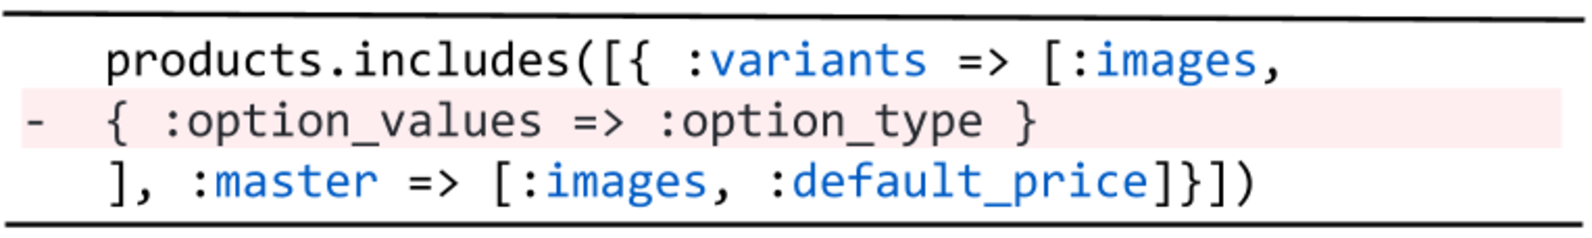
\includegraphics[width=0.7\columnwidth]{hownotto/spree5063}
  \caption{Inefficient eager loading in Spree}
  \label{fig:spree5063}
  \vspace{-0.25in}
\end{figure}

%When loadING a \texttt{product}, the corresponding \texttt{variants} and its \texttt{option\_values} and \texttt{option\_types} will be retrieved together. It is complained that it can cause the ruby process to lock up on large data sets (405 \texttt{products}/13811 \texttt{variants}/48 \texttt{optoin\_types}/948 \texttt{option\_values}). Since a variant can have many \texttt{option\_values}, the variant on average could have 20 \texttt{option\_values}. In total, there could be 276220 \texttt{option\_values} to load.  %Furthermore, ``eager loading'' may retrieve data which will never be used by the application,
%\shan{is it true?}.
%\cong{N+1 is a well-known problem. I think we may need to go deeper into the cause. As for lazy loading, why would developers load more data than needed? (programmability or modularity?)} 

\vspace{-0.08in} 
\paragraph{\bf{Inefficient updating}}
Like the ``N+1'' problem, developers would issue N queries to update N records separately (e.g., \texttt{objects.each |o| o.update end}) rather than merging them into one update (e.g., \texttt{objects.update\_all}). This is reported in Redmine and Spree, and our static checker (to be discussed in Section~\ref{sec:dis}) finds this to be common in the latest versions of 6 out of the 12 studied applications. 
\vspace{-0.22in} 
\subsubsection{Unnecessary Data Retrieval (UD)} 
%Since ORM frameworks are not aware of the high level application semantics. They cannot figure out how developers will use the data returned from the DBMS. Thus,  providing optimal data retrieval approach is not an easy job.
Unnecessary data retrieval happens when software retrieves persistent data that is not used later. Prior work has identified this problem in applications built using both Hibernate~\cite{chen:se16:redundantData} and Rails~\cite{yan:cikm17}. In our study, we find this continues to be a problem in one problematic action in the latest version of Gitlab and 9 performance issue reports.
Particularly, fixing the unnecessary data retrieval in the latest 
version of Gitlab can drop the end-to-end loading time of its 
\texttt{Dashboard/Milestones/index} page from 3.0 to 1.1 seconds in our experiments.
We also see some unnecessary data retrieval caused by simple misuses
of APIs that have similar names --- \texttt{map(\&:id)} retrieves the whole
record and then returns the \texttt{id} field, yet \texttt{pluck(:id)} only
retrieves the \texttt{id} field. 
%TODO \alvin{This is a weak point given (our own) prior work and also we are not showing code. I suggest removing it if we need space.}
%there are 2 cases caused by map vs pluck
\vspace{-0.08in} 
\subsubsection{Inefficient Rendering (IR)}
\label{sec:iffirender}
IR reflects a trade-off between readability and performance when a view file renders a set of objects. It has not been studied before.

Given a list of objects to render, developers often 
%implement a function, or use an existing library function
use a library function, like \texttt{link\_to} on Line 4 of Figure~\ref{fig:partialA},
to render one object and encapsulate it in a partial view file
such as \texttt{\_milestone.html.haml} in Figure~\ref{fig:partialA}.
Then, the main view file \texttt{index.html.haml} simply applies the
partial view file repeatedly to render all objects. 
The inefficiency is that a rendering function like \texttt{link\_to}
is repeatedly invoked to generate very similar HTML code. Instead,
the view file could generate the HTML code for one object,
and then use simple string substitution, 
such as \texttt{gsub} in Figure~\ref{fig:partialB}, to quickly 
generate the HTML code for the remaining objects, avoiding redundant
computation. The latter way of
rendering degrades code readability, but improves performance substantially
when there are many objects to render or with complex rendering functions.

Although slow rendering is complained, such transformation has not yet been proposed by issue reports. Our profiling finds such optimization speeds up 5 problematic actions by 2.5$\times$ on average.
%This type of problems does not exist in the 140 issue reports that we studied. 
%However, our profiling finds the above transformation to speed up 5 problematic actions by 2.5$\times$ on average. 

\begin{figure}
\centering
\label{fig:sl}
    \begin{subfigure}
    \centering
        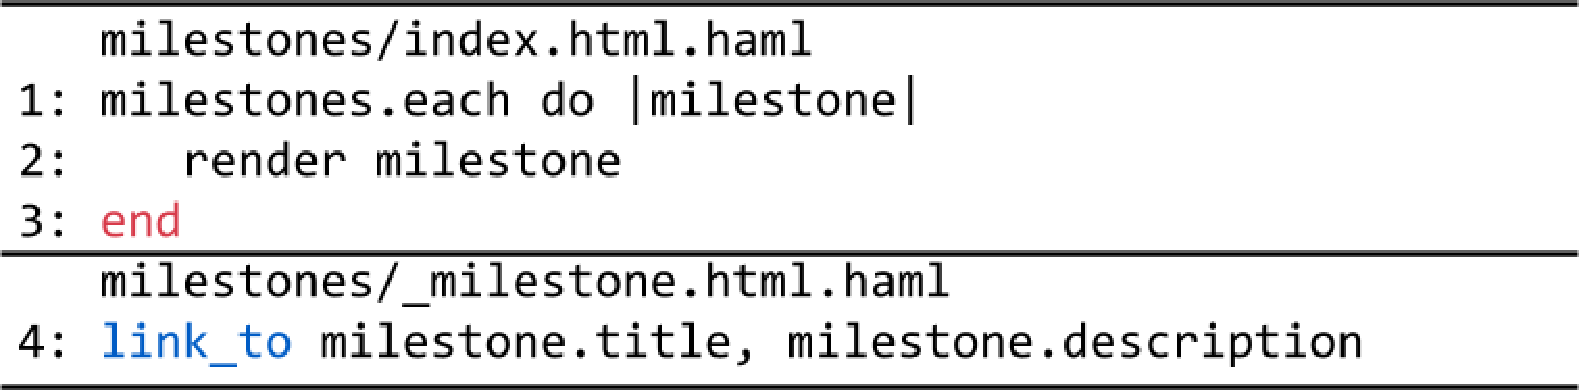
\includegraphics[width=0.4\linewidth]{hownotto/partialA.pdf}
       \caption{Inefficient partial rendering}
         \label{fig:partialA}
    \end{subfigure}
    \begin{subfigure}
        \centering
        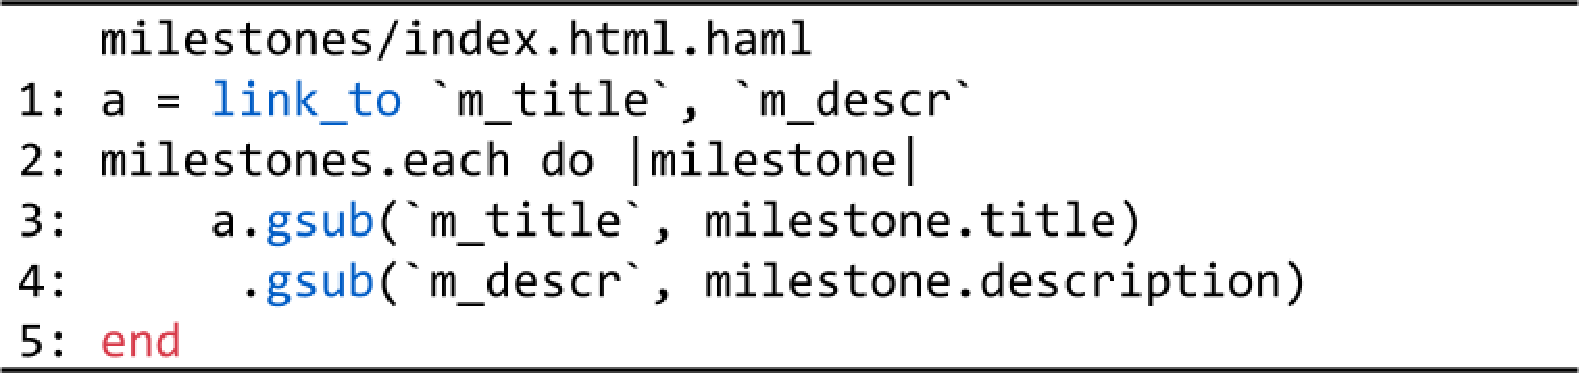
\includegraphics[width=0.4\linewidth]{hownotto/partialB.pdf}
       \caption{Efficient partial rendering}
        \label{fig:partialB} 
    \end{subfigure}
\caption{Inefficient partial rendering in Gitlab}
\end{figure}

\subsection{Database Design Problems}
\label{causes:db}

Another important cause of performance problems is suboptimal database design. Fixing it requires changing the database schema.
%Sometimes, the root cause of a performance problem is about database table design. Consequently, fixing these problems requires modifying schema and model files in ORM applications.
\vspace{-0.08in} 
\subsubsection{Missing Fields (MF)}
\label{sec:addfield}
%ORM frameworks encourage developers to maintain all classes to be stored in the database as model classes \alvin{what does Rails call such classes?} \alvin{find something to cite if possible regarding standard practices} for modularity and code maintenance. 
Deciding which object field to be physically stored in database is a non-trivial part of database schema design. %Similarly, which fields should be persistent in a model class is not always clear. 
If a field can be easily derived from other fields, storing it in database may waste storage space and I/O time when loading an object; if it is expensive to compute, not storing it in database may incur much computation cost. Deciding when a property should be stored persistently is a general problem that has not been studied in prior work.


%Not all applications make the best decision on whether to physically store a field.
For example, when we profile the latest version of Openstreetmap~\cite{openstreetmap}, a collaborative editable map system, 
we find that a lot of time is spent on generating a \texttt{location\_name} string for every diary based on the diary's longitude, latitude, and language properties stored in the \texttt{diary\_entry} table. Such slow computation results in a problematic action taking 1 second to show only 20 diaries.
However, the \texttt{location\_name} is usually a short string and remains the same value since the location information for a diary changes infrequently. Storing this string physically as a database column avoids the expensive computation. We evaluate this optimization and find it reducing the action time to only 0.36 second.
%we find its 
%\texttt{diary\_entry/index} action problematic, taking 1.00 seconds to list the text abstract of only 20 diaries. 
%We then find that most of the time is spent in generating a \texttt{location\_name} string for every diary based on the diary's longitude, latitude, and language properties stored in the \texttt{diary\_entry} table. 

%For example, given 
%\{57.7089$^{\circ}$N, 11.9746$^{\circ}$E, English\},
%``Gothenburg, Sweden'' will be computed for display.
%This computation is not cheap, and the size of the \texttt{location\_name} string is negligible for every diary. Furthermore, the location information of a diary almost never changes once created and tends to be displayed for many times.
%Once we add a \texttt{location\_name} column into the \texttt{diary\_entry} table, the server time of \texttt{diary\_entry.index} drops from 1.00 seconds to 0.36 seconds. 

%longi, lati, scale, language
%diary entry.index
%text list
%

We observe similar problems in the bug reports of Lobster, Spree, and Fallingfruit, and in the latest version of Redmine, Fallingfruit, and Openstreetmap. Clearly, developers need help on 
performance estimation to determine which fields to persistently store in database tables. 
%We outline this as part of future research problems in Section \ref{sec:dis}.

%\cong{Interesting. So whether to materialize a field matters to the performance, right? But seeing from the table there is only one case. Will you be able to find more examples?}
\begin{comment}
\subsubsection{To Associate or Not to Associate (Missing Associations)} 
\label{sec:addassoc}

Rails, like other ORM frameworks, allows developer to declare whether two %persistently stored 
classes have no relationships, or have one or multiple
\texttt{OneToOne}, \texttt{OneToMany}, \texttt{ManyToOne} association relationship(s) between them. Determining the association relationships is another hard task for developers. 
%as different designs have different implications for the performance of the resulting queries along with storage costs. 
\shan{TODO: rewrite the next few sentences.}
Prior work~\cite{bag:tradeoff} attempts to reconcile the trade-off between time and space performance among different object-relational mapping strategies. However, this only helps when an application is designed from scratch. For mature applications, 
it will takes a lot of effort to find the missed association.


Figure \ref{fig:spree7511} shows an example of developers adding a \texttt{has\_one} association to improve performance (\texttt{Spree-7511}).
At first, developers discovered an 
N+1 query problem (Section
\ref{sec:iffidata}) in a view file
\texttt{\_order\_details.html.erb}. As shown in Figure \ref{fig:spree7511}, this view file first loads an array of {\tt shipments} from the {\tt shipment} table, and then, for each individual shipment object \texttt{sm} in this array,
a \texttt{selected\_shipping\_rate} function is invoked to issue a 
\texttt{SELECT} query to the {\tt ShippingRate} table.
In order to batch these N+1 queries to 
{\tt shipment} table and {\tt ShippingRate} table together into one query, developers decided to add
\texttt{selected\_shipping\_rate} as an association between these two tables/model-classes, denoted by the added
\texttt{has\_one} line in Figure \ref{fig:spree7511}. 
This new association allows all the shipments' 
selected shipping rates to be loaded in one query using the \texttt{includes} shown in the patch of \texttt{\_order\_Details.html.erb}. 

Note that, adding an association usually requires adding one table's primary key
into the other table as a foreign key, which incurs extra storage cost. 
\cong{I doubt that extra storage cost is the concern. I think maybe the complicated conditional association is hard to use/not intuitive?}
In this example, since there was already a \texttt{has\_many}
association called \texttt{shipping\_rates} between these two classes,
the newly added association incurs almost no cost.

We have observed similar problems and patches in the bug-tracking
systems of Lobster, Spree, and Diaspora. 
We also found a similar problem in the latest version of Tracks. By
adding an extra association, the end-to-end latency of Tracks' \texttt{projects/review} drops
from 0.98 seconds to 0.65 seconds.

%\shan{need a better explanation. maybe start from explicitly explaining $N+1$ problems. maybe we can mention class cohesion ... point out that this is not a db problem}
\begin{figure}[h]
  \centering
  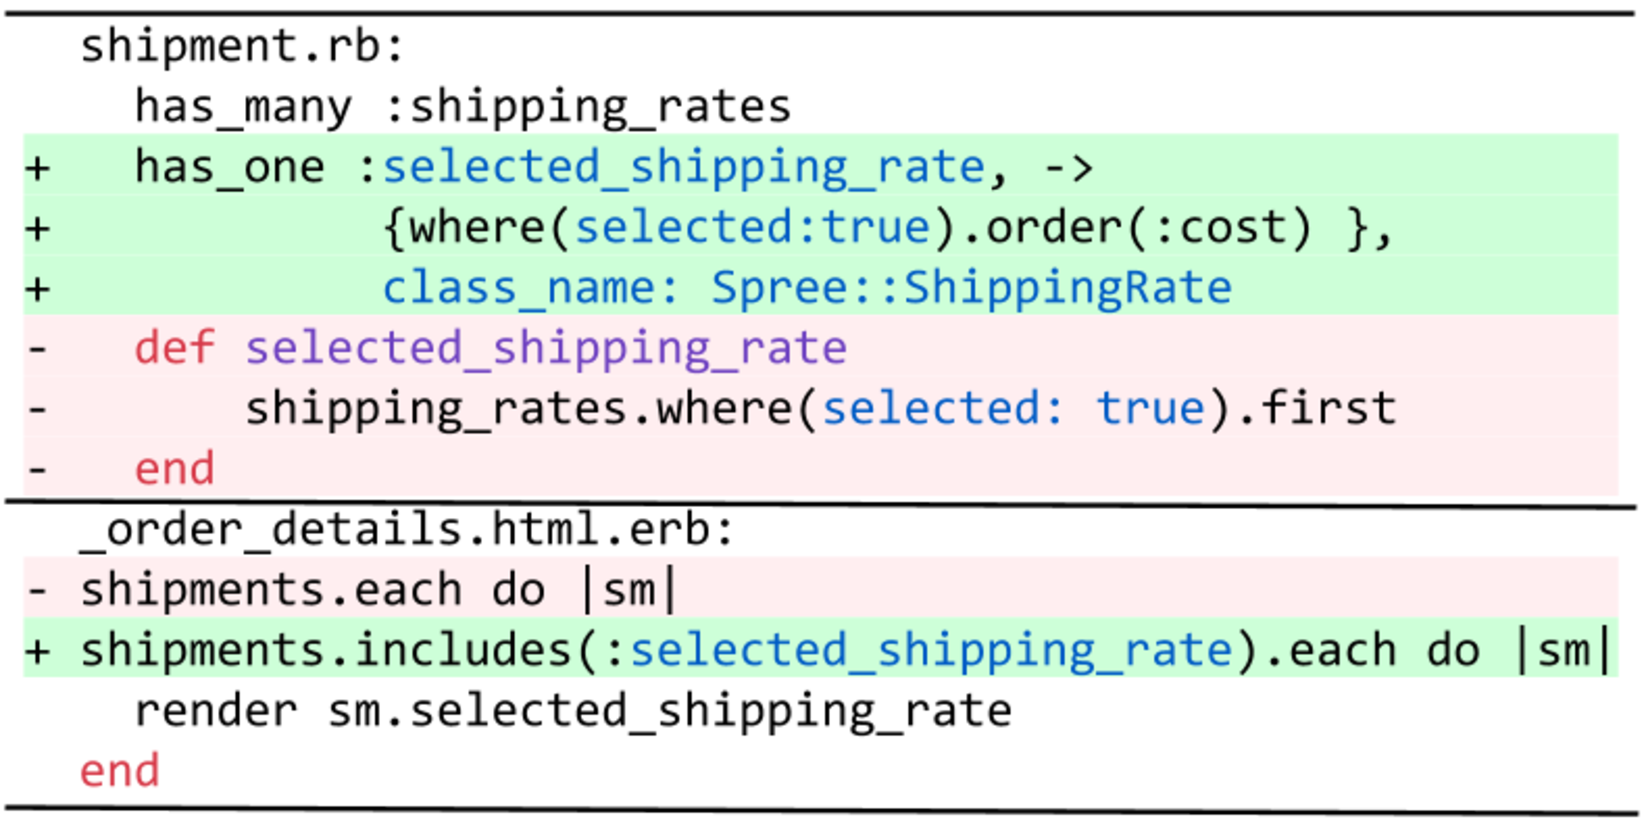
\includegraphics[width=1\columnwidth]{figs/spree7511}
  \caption{Adding association to enable eager loading (Spree)}
  \label{fig:spree7511}
  
\end{figure}
\end{comment}
\vspace{-0.10in}
\subsubsection{Missing Database Indexes (MI)}

Having the appropriate indexes on tables is important for query processing and is a 
well-studied problem \cite{Ullman:1997}. 
As shown in Table \ref{tab:freq}, missing index is the most common performance problem reported in ORM application's bug tracking systems. However, it only appears in three out of the \numpactions problematic actions in latest versions.
We speculate that ORM developers
often do not have the expertise to pick the optimal indexes at the design
phase and hence add table indexes in an incremental way depending on
which query performance becomes a problem after deployment.
%In most of the missing-index issues, an index was added to improve the performance of join queries (7 out of 11), particularly join queries whose \texttt{join} clause contains more than 10 columns (xx out of xx) Missing single and multi-column indexes are both common (about 2:1 ratio)
%.
%missing indexes were so common for several reasons. 
%First, developers of database-backed web applications are often not database optimization experts 
%(partially due to the ORM hiding the database away as an abstraction), and picking the optimal indexes requires understanding the semantics of the application and also how each call to the ORM framework is translated to queries.
%Furthermore, even if developers have the required expertise, they might worry about the cost (in terms of disk and memory space) for creating indexes.
%especially when a table already contains several other indexes. xxx. 
%In fact, xx out of xx missing-index tables in our study were initially released with only one index on its primary key, and only when query performance becomes a problem after deployment will indexes be added in subsequent versions of the application.




\subsection{Application Design Trade-offs}
\label{sec:appdesign}

Developers fix 33 out of the \numissues issue reports by adjusting application display or removing costly functionalities. 
We find similar design problems in latest
versions of 7 out of 12 ORM applications. It is impractical to
completely automate display and functionality design. 
However, our study
shows that ORM developers need tool support, which does not exist yet, to be more informed about the performance implication of their application design decisions.
%found no effectively way to solve the performance problems unless developers throw away some unworthy functionality.
\vspace{-0.10in} 
\subsubsection{Content Display Trade-offs (DT)}
In our study, the most common cause for scalability problems is that a controller action displays \textit{all} database records satisfying certain condition in one page. When the database size increases, the corresponding page takes a lot of time to load due to the increasing amount of data to retrieve and render. This problem contributes to 15 out of the
34 problematic actions that do not scale well in our study. It also appears in 7 out of \numissues issue reports, and is \textit{always} fixed by pagination, i.e., display only a fixed number of records in one page and allow users to navigate to remaining records. 

%As an example, the \texttt{products/index} page in \texttt{Ror\_ecommerce} renders all \textit{products} that are stored in the database. As the number of products increases, the time taken to render the page will increase as well. In practice, users often do not need to see all contents within one page. (e.g., they may only want to see the most popular products). By rendering products by pagination (showing only \alvin{XXX} per page), we find that performance can be improved by $5\times$.

\textcolor{black}{ For example, in \texttt{Diaspora-5335} %named ``\texttt{Paginate cont-}\texttt{acts}'', 
developers used the \texttt{will\_paginate} library~\cite{gem:paginate} to render 25 contacts per page and allow users to see the remaining contacts by clicking the navigation bar at the bottom of the page, instead of showing all contacts within one page as in the old version.
%\texttt{Redmine}, on the other hand, solves a similar problem in 
%\texttt{Redmine-5286} by letting users specify how many issues they want to see within one page.
Clearly, good UI designs can both enhance user experience and improve application performance.} 

%Pagination 
%is widely used in webpage displaying; there are also Rails library support for implementing pagination \cite{gem:paginate}. 
Unfortunately, the lack of pagination still widely exists in latest versions
of ORM applications in our study. This indicates that ORM developers need 
database-aware performance-estimation 
support to remind them of the need to use pagination in webpage design.
\vspace{-0.08in}

\subsubsection{Application Functionality Trade-offs (FT)}
\label{sec:simplifyfeatures}
%When designing the application, without knowing the real workload, it's hard for designers to know the exact time consumed on certain functional feature. As a result, the application may contain some features that cause severe performance problems without bringing much functionality appealing.
%This is particularly a problem in ORM applications, because it is often difficult for developers to know whether and what queries are issued underlying Ruby code, not to mention estimating the query cost.

It is often difficult for ORM developers to estimate performance of a new application feature given that they need to know what queries will be issued by the ORM, how long these queries will execute, and how much data will be returned from the database. In our study, all but two applications have performance issues fixed by developers through removing functionality. 

For example, \texttt{Tracks-870} made a trade-off between performance and functionality by removing a sidebar on the resulting page. This side bar retrieves and displays all the projects and contexts of the current user, and costs a lot of time for users who have participated in many projects.
In the side-bar code, the only data-related part is simply a \texttt{@sidebar.active\_projects} expression, which seems like a trivial
heap access but actually issues a \texttt{SELECT} query and retrieves a lot of data from the database.

As another example, our profiling finds that the \texttt{story.edit} action in the latest version of Lobsters takes 1.5 seconds just to execute one query that determines whether to show the \texttt{guidelines} for users when they edit stories, while the entire page takes 2 seconds to load altogether. Since the  \texttt{guidelines} object only takes very small amount of space to show on the resulting page, removing such checking has negligible impact to the application functionality, yet it would speed up the loading time of that page a lot. 


%\texttt{sidebar} to show the \texttt{actions} and \texttt{contexts} and finally decide the remove \texttt{sidebar}.

In general, performance estimation for applications built using ORMs is important yet has not been done before. It is more difficult as compared to traditional applications due to multiple layers of abstraction. 
We believe combining static analysis with query scalability estimation \cite{armbrust:sigmod13:scale, fan:pods2014:scale} will help developers estimate application performance, as we will discuss in Section \ref{sec:dis}. 
%estimate performance and scalability of ORM code snippets. Including that feature in IDE could greatly help developers in their ORM software design. 


\begin{comment}
\subsection{Potential Solutions}


\subsubsection{Ruby Code Optimization}

\textbf{use more efficient API}
\textbf{use eager loading to prefetch the data}
\textbf{partial to template}
\subsubsection{DB optimization}

\textbf{Add index}
\textbf{Table denormalization}
\subsubsection{Ruby code re-writing}
\textbf{ Paginating}
\end{comment}






\section{Fixing the Inefficiencies}
\label{sec:opt}

After identifying the performance inefficiencies in the \numpactions problematic actions across the 12 studied applications, we manually fix each of them and measure how much our fixes improve the performance of the corresponding application webpages. Our goal is to quantify the importance of the anti-patterns discussed in Section \ref{sec:causes}. 

\subsection{Methodology}
We use the same 20,000-record database configuration used in profiling to measure performance improvement.
For a problematic action that contains multiple inefficiency problems, we fix one at a time and report the speedup for each individual fix.
To fix API-use problems, we change model/view/control files that are related to the problematic API uses; to add missing indexes or fields, we change corresponding Rails migration files; to apply pagination, we use the standard \texttt{will\_paginate} library~\cite{gem:paginate}. We carefully apply  fixes to make sure we do not change the program semantics.
Finally, for two actions in Lobster, we eliminate the expensive checking about whether to show user guidelines, as discussed in Section \ref{sec:simplifyfeatures}.
%We will accumulate the optimization step by step. For example, $HomeController.recent$ action is slowed down by two redundant computation called \texttt{r1} and \texttt{r2}, after optimization \texttt{o1} which removes removing \texttt{r1}, the execution time is reduced from 3782 to 2045, and after optimization \texttt{o2} which removes \texttt{r2}, the execution is reduced from 2045 to 1013. As a result, the speed-up of \texttt{o1} is 1.8 $\times$, and the speed-up of \texttt{o2} is 2 $\times$. We will count \texttt{o1} and \texttt{o2} separately in Figure \ref{speedup}.
\begin{figure}
\centering
\label{fig:sl}
\begin{subfigure}
% \subfigure[Server-time speedup ($\times$)]{
\centering
    \includegraphics[width=0.4\linewidth]{hownotto/speedup}
   \caption{Server-time speedup ($\times$)}
    \label{fig:speedup}
\end{subfigure}
% }
% \subfigure[Line of code changes]{
\begin{subfigure}
    \centering
    \includegraphics[width=0.4\linewidth]{hownotto/loc}
   \caption{Line of code changes}
    \label{fig:loc}       
\end{subfigure}
% }
\caption{Performance fixes and LOC involved}
\end{figure}

\subsection{Results}
In total, \numacissues fixes are applied across 39 problematic actions \footnote{Among the 40 problematic actions identified by our profiling, 1 of them (from GitLab) spends most of its time in file-system operations and  cannot be sped up unless its core functionality is modified. 
} to solve the \numacissues problems listed in Table \ref{tab:freq}.
\vspace{-0.08in} 
\paragraph{\bf Speedup of the fixes}
Figure \ref{fig:speedup} shows the amount of server-time speedup and the sources of the speedup broken down into different anti-patterns as discussed in Section \ref{sec:causes}.

Many fixes are very effective. About a quarter of them achieve more than 5$\times$ speedup, and more than 60\% of them achieve more than 2$\times$ speedup. Every type of fixes
has at least one case where it achieves more than 2$\times$ speedup. 
%Although never providing more than 5X speedups, changing loading strategy provides more than 4X speedups in four cases. 
The largest speed-up is around 39 $\times $ achieved by removing unnecessary feature in \texttt{StoriesController.new} action in Lobsters, i.e., the example we discussed in Section \ref{sec:simplifyfeatures}. 

There are 40 fixes that alter neither the display nor the functionality of the original application. That is, they fix the anti-patterns discussed in Section \ref{causes:api} and \ref{causes:db}. They
achieve
an average speedup of 2.2$\times$, with a maximum of 9.2$\times$ speedup by adding missing fields in \texttt{GanttsController.show} from Redmine.

For all 39 problematic actions, many of which benefit from more than one fix, their average server time is reduced from \serverbefore seconds to \serverafter seconds, and the corresponding end-to-end page loading time is reduced from \eoebefore seconds to \eoeafter seconds, including client rendering and network communication. In other words, by writing code that contains the anti-patterns discussed earlier, developers degrade the performance of their applications by about $6\times$.
%\shan{we probably also should report the total server time and end-to-end time of the 44 actions before and after the optimization. do you have that figure?}

We have reported these 64 fixes to corresponding developers. So far, we have received developers' feedback for \numconfirmedpaissues of them, all of which have been confirmed to be true performance problems and \numfixedpaissues have already been fixed based on our report.%\shan{TODO: discuss why many have no feedback?}\junwen{For those related to API design, maybe it's hard for developers to give answer soon}
\vspace{-0.08in} 
\paragraph{\bf Simplicity of the fixes}
Figure \ref{fig:loc} shows the lines of code changes required to implement the fixes. 
The biggest change takes 56 lines of code to fix (for an inefficient rendering (IR) anti-pattern), while the smallest change requires only 1 line of code in 27 fixes. More than 78\% of fixes require fewer than 5 lines. In addition, among the fixes that improve performance by 3$\times$ or more, more than 90\% of them take fewer than 10 lines of code. Around 60\% of fixes are intra-procedural, involving only one function.  
%\shan{hmm, the lines of code are actually bigger than i expected. need discussion.}\shan{please also report inter-procedural changes vs intra-procedural changes.} 
\begin{comment}
\begin{figure}[h]
  \centering
  \includegraphics[width=1\columnwidth]{figs/speedup}
  \caption{Application server-time speedup after fixes\shan{to fix anti-pattern captions later, same for next figure}\junwen{done}
  }

  \label{speedup}
\end{figure}

\begin{figure}[h]
  \centering
	\includegraphics[width=1\columnwidth]{figs/loc}
  \caption{Lines of code in performance fixes \alvin{move legend into the graph? I think we have room}}

  \label{locchange}
\end{figure}
\end{comment}


These results quantitatively show that there is still a huge amount of inefficiency in 
real-world ORM applications. Much inefficiency can be removed through few lines of code changes.
 A lot of the fixes can potentially be automated, as we will discuss in Section \ref{sec:dis}.

\begin{comment}
\subsection{Automate Solutions}
\subsubsection{How complex are the changes that developers apply to optimize their programs}

\textbf{  Loc change}
\textbf{  program complexity change}

\subsubsection{Are there common patterns can be automated}

\end{comment}

\section{Finding more API misuses}
\label{sec:staticChecker}
\newcommand*\circled[1]{\tikz[baseline=(char.base)]{
            \node[shape=circle,draw,inner sep=1.5pt] (char) {#1};}}
 \newcommand*\smallcircled[1]{\tikz[baseline=(char.base)]{
            \node[shape=circle,draw,inner sep=1pt] (char) {#1};}}
            
Some problems described in Section~\ref{causes:api} are about simple API misuses. We identify 9 such simple misuse patterns, as listed in Table \ref{tab:badapi}, and implement a static analyzer to search for their existence in latest versions of the 12 ORM applications. 
Due to space constraints, we skip the implementation details. 
%through regular expression matching. 
To recap, these 9 API patterns cause performance losses due to ``An Inefficient Query'' 
({\footnotesize \circled{1}, \circled{2}, \circled{3}}), 
``Moving Computation to the DBMS''
({\footnotesize \circled{7}, \circled{8}, \circled{9}}),
``Moving Computation to the Server''
({\footnotesize \circled{5}}),
``Inefficient Updating''
({\footnotesize \circled{4}}), and
``Unnecessary Data Retrieval''
({\footnotesize \circled{6}}), as discussed in Section~\ref{causes:api}. 

\begin{table}
\vspace{-0.05in}
\centering
\caption{API misuses we found in the latest versions}
{\small
\label{tab:badapi}
\begin{tabular}{l@{\hspace{0.01in}}rrrrrrrrrr}
\toprule
App. & \circled{1}  & \circled{2}   & \circled{3} & \circled{4} & \circled{5}  & \circled{6}  & \circled{7}  & \circled{8} & \circled{9} & SUM \\
\midrule
Ds      & 8  & 61  & 0 & 0 & 6  & 6  & 3  & 0 & 1 & 85  \\
\midrule
Lo      & 1  & 38  & 0 & 0 & 0  & 5  & 1  & 0 & 0 & 45  \\
\midrule
Gi      & 7  & 3   & 0 & 1 & 6  & 3  & 3  & 0 & 0 & 23  \\
\midrule
Re      & 3  & 32  & 0 & 1 & 16 & 7  & 0  & 0 & 0 & 59  \\
\midrule
Sp      & 2  & 10  & 0 & 0 & 0  & 0  & 7  & 1 & 0 & 20  \\
\midrule
Ro      & 0  & 7   & 0 & 1 & 1  & 0  & 2  & 0 & 0 & 11  \\
\midrule
Fu      & 0  & 0   & 0 & 0 & 2  & 0  & 0  & 0 & 0 & 2   \\
\midrule
Tr      & 4  & 22  & 0 & 1 & 3  & 0  & 0  & 0 & 0 & 30  \\
\midrule
Da      & 5  & 42  & 1 & 1 & 0  & 8  & 0  & 0 & 0 & 57  \\
\midrule
On      & 10 & 60  & 0 & 0 & 6  & 0  & 0  & 0 & 0 & 76  \\
\midrule
FF      & 2  & 0   & 0 & 2 & 0  & 0  & 0  & 0 & 0 & 4   \\
\midrule
OS      & 0  & 12  & 0 & 0 & 2  & 2  & 0  & 0 & 0 & 16  \\
\midrule
SUM     & 42 & 287 & 1 & 7 & 42 & 31 & 16 & 1 & 1 & 428\\
\bottomrule
\end{tabular}
}

{\footnotesize 
\begin{tabular}{ll}
\smallcircled{1}: \texttt{any?} $\Rightarrow$ \texttt{exists?} & \smallcircled{2}: \texttt{where.first} $\Rightarrow$ \texttt{find\_by} \\
\smallcircled{3}: \texttt{*} $\Rightarrow$ \texttt{*.except(:order)} & \smallcircled{4}: \texttt{each.update} $\Rightarrow$ \texttt{update\_all} \\
\smallcircled{5}: \texttt{.count} $\Rightarrow$ \texttt{.size} & \smallcircled{6}: \texttt{.map} $\Rightarrow$ \texttt{.pluck} \\
\smallcircled{7}: \texttt{pluck.sum} $\Rightarrow$ \texttt{sum} & \smallcircled{8}: \texttt{pluck + pluck} $\Rightarrow$ \texttt{SQL-UNION}\\
\multicolumn{2}{l}{\smallcircled{9}: \texttt{if exists? find else create end} $\Rightarrow$ {find\_or\_create\_by}}\\
\end{tabular}
 \\

\par} 
\end{table}

As shown in Table \ref{tab:badapi}, 
every API misuse pattern still exists in at least one application's latest version. Worse, 4 patterns each occur in over 30 places across more than 5 applications. 
We have checked all these 428 places and confirmed each of them. For further confirmation, we posted them to corresponding application's bug-tracking system, and every category has issues that have already been confirmed by application developers.
%\junwen{For each pattern, we have received confirmation from at least one application developers that what we found are indeed API misuses.} 
\numconfirmedapi API misuses have been confirmed, and \numfixedapi already fixed in their code repositories based on our bug reports. None of our reports has been denied. %Furthermore, \circled{1} and \circled{5} have already been merged to their repository in Onebody.

Only 3 out of these 428 API misuses coincide with the 64 performance problems listed in Table~\ref{tab:freq} and fixed in Section~\ref{sec:opt}. This is because most of these 428 cases do not reside in the 40 problematic actions that we have identified as top issues in our profiling. However, they do cause unnecessary performance loss, which could be severe under workloads that differ from those used in our profiling.

In sum, the above results confirm our previously identified issues, and furthermore indicate that simple API misuses are pervasive across even the latest versions of these ORM applications.
Yet, there are many other types of API misuse problems discussed in Section \ref{causes:api} that cannot be detected simply
through regular expression matching and will require future research to tackle.

\begin{comment}

\begin{table}
\caption{API misuses in latest versions}
\label{tab:badapi}
{
\begin{tabular}{rl}
\toprule
Misuse Pattern & Applications\\
\midrule
\texttt{count(*)>0} $\Rightarrow$ \texttt{exists?} & {Ds$_9$, Lo$_1$, Gi$_7$, Re$_3$, Sp$_2$, Tr$_4$, Da$_5$, On$_10$, FF$_2$}\\
\texttt{where.first} $\Rightarrow$ \texttt{find\_by} & {}\\
\texttt{*} $\Rightarrow$ \texttt{*.except(:order)} & \\
\texttt{each.update} $\Rightarrow$ \texttt{update\_all} & \\
\texttt{.count} $\Rightarrow$ \texttt{.size} & Red$_3$\\
\texttt{.map} $\Rightarrow$ \texttt{.pluck} & Red$_3$\\
\texttt{.map} $\Rightarrow$ \texttt{.pluck} & Red$_3$\\
\texttt{pluck.sum} $\Rightarrow$ \texttt{sum} & Red$_3$\\
\texttt{array + array} $\Rightarrow$ \texttt{UNION} & Red$_3$\\

\texttt{if exists? } $\Rightarrow$ \&{}\\

\texttt{find\_or\_create\_by} & Red$_3$\\

\bottomrule
\end{tabular}
}
{\footnotesize \\ Subscript: \# of misuses in the latest version of an application \par}
\end{table}
\end{comment}


\section{Discussion}
\label{sec:dis}

%Earlier sections have discussed various performance anti-patterns that widely exist in ORM applications, and also discussed what problems need future research to look at. In the section, we summarize some common themes for future research.

In this section, we summarize the lessons learned and highlight the new research opportunities that are opened up by our study.

%\vspace{-0.05in}
\vspace{-0.09in}
\paragraph{\bf{Improving ORM APIs}}Our study shows that many misused APIs have confusing names, as listed in Table \ref{tab:badapi}, but are translated to different queries and have very different performance. 
%As another example, the {\tt first} query API orders tuples by primary key which is not reflected by the function name and is usually unnecessary.
Renaming some of these APIs could help alleviate the problem.
Adding new APIs can also help developers write well-performing code
without hurting code readability. 
For example, if Rails provides native API support for taking union of 
two queries' results like Django \cite{django} does, there will be
fewer cases of inefficient computation, such as those discussed in Section~\ref{sec:inefficomp}.
%inefficient {\tt pluck(:id)+pluck(:id)} problems.
As another example, better rendering API supports could help eliminate inefficient partial render problem discussed in 
Section~\ref{sec:iffirender}.
%; it applies to the \alvin{?}
To our best knowledge, no ORM framework provides this type of rendering support.
%This also applies to utilizing the database query log and query plan to improving database design like adding missed index.
%\cong{I change the example. bulk create/delete is not a problem in Django.}
%This also applies to the inefficient data accessing problem discussed
%in Section~\ref{sec:iffidata}, where the lack of bulk record creation/deletion/update APIs in Rails inevitably encourages 
%performance problems. New APIs would help eliminate
%such inefficiency \shan{how does other ORM do on this?}. \alvin{I have the same question.}

%For instance, Gitlab uses
%``EXPLAIN ANALYZE'' to check query plan and add index accordingly,
%and such feature may be wanted by many developers since missing
%index is a very common problem and does not have completely automatic
%solution\shan{are we suggesting people all use gitlab tool?}. Another example feature is recursively deleting associate records
%without issueing N+1 query, which is not supported by current API\shan{don't understand. what does this mean?}.
%A third example feature is building template for partial rendering\shan{what does this mean?}.
%Adding an API to support template in extension to existing {\tt %render\_partial}
%API can reduce much redundant computation in rendering similar records.
%\cong{I'm not sure which example is better so I just list all of them here.}
\vspace{-0.12in}
\paragraph{\bf{Support for design and development of ORM applications}}
Developers need help to better understand the performance of their code, especially the parts that involve ORM APIs.
%ORM APIs and the potential cost of ORM code, because currently the time-consuming part of the application is all hidden by the ORM framework. 
%They can no longer just focus on explicit loops in performance estimation.
They should focus on not only loops but ORM library calls (e.g., joins) in performance estimation, since these calls often execute database queries and can be expensive in terms of performance.
Building static analysis tools that can estimate performance 
and scalability of ORM code snippets will alleviate some of the API misuses.
More importantly, this can help developers design 
better application functionality and interfaces, as discussed in Section~\ref{sec:appdesign}. 

Developers will also benefit from tools that can aid in database design, such as suggesting 
fields to make persistent, as discussed in Section~\ref{causes:db}.
While prior work focuses on index design~\cite{autoadmin}, little has been done on aiding developers to determine which fields to make persistent.
%In contrast to traditional database design tools that relies of query logs to infer application semantics~\cite{autoadmin}, 
As the ORM application already contains information on how each object field is computed and used,
%database field is updated and used to compute other properties, this 
this provides a great opportunity for program analysis to further help in both aspects.
%help with database schema design, suggesting which field to be stored persistently.
%suggesting adding or deleting fields.
%this... Traditional design tools also has query log as representative workload. 'query semantic' is in query and need not to infer?}

%Our study indicates that it is possible to build such design-time support.
%recommend the result may better be saved to database.

%\shan{moved here from index}
%Interesting, we notice that Gitlab developers already built a testing tool \cite{sherlock} targeting this problem. This tool leverages postgresql's 
%\texttt{EXPLAIN ANALYZE} functionality to analyze all the query plans 
%of queries issued during testing and see if a column is missing index.
%The above solution is useful but requires
%a large amount of profiling. Future research
%can potentially build static checking tools that xxx.
\vspace{-0.12in} 
\paragraph{\bf{Compiler and runtime optimizations}}
While some performance issues are related to developers' design decisions, we believe that others can be detected and fixed automatically. Previous work has already tackled 
some of the issues such as pushing computation down to database through query synthesis \cite{cheung:pldi13}, query batching \cite{cheung:sigmod14:sloth, dbridge:tkde15}, and avoiding
unnecessary data retrieval \cite{chen:se16:redundantData}. There are still many 
automatic optimization opportunities that remain unstudied. This ranges from checking for API misuses, as we discussed in Section~\ref{sec:staticChecker}, to more sophisticated 
database-aware optimization techniques to remove unnecessary computation (Section~\ref{sec:uncomp}) and inefficient queries (Section~\ref{sec:inefficomp}). 

Besides static compiler optimizations, runtime optimizations or trace-based optimization for ORM frameworks are further possibilities for future research, such as automatic pagination
for applications that render many records,
runtime decisions to move computation between the server and the DBMS, 
runtime decisions to switch between lazy and eager loading,
and 
%can be made whether to perform a computation in memory or to issue a database query, depending on whether the data is already loaded;
runtime decisions about whether to %perform
remove certain expensive functionalities as discussed in Section~\ref{sec:simplifyfeatures}.
%\alvin{I don't get the last one} \cong{is 'remove' better?}
Automated tracing and trace-analysis tools can help model workloads
and workload changes, which can then be used to adapt database and application designs automatically.
%missed foreign key index may be added
%automatically when the system detects that such index will be frequently used if added.
Such tools will need to understand the ORM framework and the interaction among the client, server, and DBMS.
\vspace{-0.13in} 
\paragraph{\bf{Generalizing to other ORM frameworks}}
Our findings and lessons apply to other ORM frameworks as well. The database design (Section \ref{causes:db}) and application design trade-offs (Section \ref{sec:appdesign}) naturally apply across ORMs. Most of the API use problems (Section \ref{causes:api}), like unnecessary computation (UC), data accessing (ID, UD), and rendering (IR), are not limited to specific APIs and hence are general.
While the API misuses listed in Table~\ref{tab:badapi}
may appear to be Rails specific, 
there are similar misuses in applications built upon Django ORM~\cite{django} as well: {\tt exists()} is more efficient than 
\texttt{count>0} ({\footnotesize \circled{1}}); {\tt filter().get()} is faster than 
\texttt{filter().first} ({\footnotesize \circled{2}}); {\tt clear}
\texttt{\_ordering(True)} is like 
\texttt{except(:order)} ({\footnotesize \circled{3}}); {\tt all.update} can batch updates ({\footnotesize \circled{4}}); 
{\tt len()} is faster than {\tt count()} with loaded arrays ({\footnotesize \circled{5}});  
 {\tt only()} is like {\tt pluck()}({\footnotesize \circled{6}}); 
  {\tt aggregate}
  {\tt (Sum)} is like {\tt sum} in Rails  ({\footnotesize \circled{7}}); 
   {\tt union} allows two query results to be unioned in database ({\footnotesize \circled{8}}); 
{\tt get\_or\_create} is like 
{\tt find\_or\_create\_by} in Rails 
({\footnotesize \circled{9}}). 
We sampled 15 issue reports each from top 3 popular Django applications on GitHub. As shown below, these 45 performance issues fall into the same 8 anti-patterns our \numissues Rails issue reports fall into: 
%Furthermore, for {\bf every} anti-pattern observed in Rails issue reports, we also observed it in issue reports from top 3 popular Django applications on GitHub \cite{redash,zulip,django-cms}:
%IC \cite{zulip3629}, UC \cite{cms4461}, ID \cite{cms1117}, UD \cite{zulip375}, MF \cite{cms912}, MI \cite{zulip5214}, DT \cite{redash625}, FT \cite{redash300} (many more Django examples skipped for space).

\begin{table}[h]
\centering
\footnotesize
%\caption{Number of problematic actions in each application}
\begin{tabular}{@{\hspace{0.1in}}l@{\hspace{0.1in}}l@{\hspace{0.1in}}l@{\hspace{0.1in}}l@{\hspace{0.1in}}l@{\hspace{0.1in}}l@{\hspace{0.1in}}l@{\hspace{0.1in}}l@{\hspace{0.1in}}l@{\hspace{0.1in}}}
\toprule
       & IC& UC& ID& UD& MF& MI& DT & FT\\
\midrule
Redash \cite{redash} 		& 2 & 3 & 6 & 0 & 0 & 0 & 2 & 2\\
Zulip \cite{zulip}  		& 2 & 5 & 2 & 1 & 0 & 2 & 1 & 2 \\
Django-CMS \cite{django-cms}& 0 & 9 & 3 & 0 & 1 & 0 & 1 & 1 \\
 \bottomrule
\end{tabular}
\end{table}


%TODO Out of Space
%\paragraph{\textbf{Readability vs. Efficiency}} Developers' initial reaction to the patch in Figure \ref{fig:tracks63} is that it hurts code readability. Patches to xxx actually introduce message-chain code smell. some redundant computation may be caused by fear of hurting code modularity. count vs size patch may not be optimal given the code modularity. \shan{why some problems exist in old version and still appear in latest version? }



%\vspace{-0.05in}
\section{Performance}
\label{sec:related}

\vspace{-0.025in}
\paragraph{\bf{Empirical studies}}
Previous work confirmed that performance bugs are prevalent in open-source C/Java programs
and often take developers longer time to fix than other types of bugs~\cite{song.pldi12, zaman.msr12}. Prior work~\cite{mark:se17:javascript} studied the performance issues in JavaScript projects. We target performance problems in ORM applications that are mostly related to how application logic interacts with underlying database and are very different from those in general purpose applications. 
Our recent work \cite{yan:cikm17} looked into the database performance of ORM applications and discussed how better database optimization and query translation can improve ORM application performance. No issue report study or thorough profiling was done. In contrast, our paper performs a comprehensive study on all types of performance issues reported by developers and discovered using profiling. Unnecessary data retrieval (UD), content display trade-offs (DT), and part of the inefficient data accessing (ID) anti-patterns \textcolor{black}{ are the only overlap between this study and our previous work \cite{yan:cikm17} }.
%In our previous work \cite{yan:cikm17}, we looked into the database queries of these applications and xxx\shan{Cong, can you extend?} \alvin{is this double blinded? If so we can't say in our previous work}.\junwen{It's double blind review} In this paper, we perform a thorough study on all performance issues, reported by developers and discovered by our profiling.
%In fact, only xx, xx, and xx anti-patterns overlap between our study and the previous work \cite{yan:cikm17}.

\vspace{-0.08in} 
\paragraph{\bf{Inefficiencies in ORM applications}}
Previous work has addressed specific performance problems in ORM applications, such as locating unneeded column data retrieval~\cite{chen:se16:redundantData}, N+1 query
\cite{chen:se14:antipattern}, pushing computation to the DBMS~\cite{cheung:pldi13}, and query batching~\cite{cheung:sigmod14:sloth, dbridge:tkde15, quro}. While effective, these tools do not touch on many anti-patterns discussed in our work, like unnecessary computation (UC), inefficient rendering (IR), database designs (MF, MI), functionality trade-offs (FT), and also do not completely address anti-patterns like inefficient computation (IC) and inefficient data accessing (ID). 
%there are still many problems left addressed, such as ``Inefficient Query'', ``Should Not be a Query'', ``Redundant Computation'', ``Constant Query'', ``Inefficient Eager Loading'', and database and application design tradeoff problems.
%, \cite{quro} reorders query in transactions, .
%synthetic workload generation \cite{pavlo}
%\cite{bailis.sigmod15} investigates the concurrency control in Rails applications.
%Plenty of works \cite{taoxie.ase11} \cite{Torlak2012} \cite{shadi.ase11} have been conducted to generate testing loads for DBMS.

%\shan{we need to explain the difference from the CIKM paper?}

\vspace{-0.08in}
\paragraph{\bf{Performance issues in other types of software}}
Much research was done to detect and fix performance
problems in general purpose software
\cite{song.pldi12,toddler.icse13,caramel.icse15,isil.pldi15,bloat.fse08,harry.pldi09,harry.pldi10}.
%, such as performance-sensitive API misuses
%\cite{song.pldi12}, inefficient and redundant loop computation
%\cite{toddler.icse13, caramel.icse15,isil.pldi15}, object bloat
%\cite{bloat.fse08,harry.pldi09}, low-utility data structures
%\cite{harry.pldi10}, etc.
%Some of these problems share common root causes as some of the ORM performance anti-patterns, such as redundant computation in loop.
Detecting and fixing ORM performance anti-patterns require a completely different set of techniques that understand ORM and underlying database queries.
%Redundant computation problem in regular applications \cite{song.pldi12, loop.icse17}.



\chapter{PowerStation: Detecting and Fixing Performance Inefficiencies}

\section{Overview}

Previous chapter have shown that developers often struggle at writing efficient web applications
using ORM frameworks
\cite{yan:cikm17, junwen:icse2018, chen2016finding, cheung2013optimizing}. 
Several ORM-related performance anti-patterns have been found to widely exist 
in real world database-backed web applications and lead to application inefficiencies.
%These performance problems often lead to several times' slow downs and cannot be optimized by
%state of the art object-oriented program language compilers, 
Unfortunately, many of these inefficiencies go undetected by compilers and database management systems as they focus solely on either the application code or the embedded queries, while recognizing such inefficiencies require both systems to work in tandem.
%\shan{Alvin, the first two paragraphs are reorganized to address your earlier comments}

This chapter presents PowerStation, an IDE plugin for Ruby on Rails (Rails) applications that automatically detects ORM-related
performance problems and suggests fixes for them.
It makes two contributions.
First, we build a database-aware static analysis framework for Rails applications. 
The current PowerStation prototype can already detect 6 common
ORM performance anti-patterns and generate patches for 5 of them. 
These anti-patterns include loop invariant query, dead store query, unused data retrieval, unoptimized common subexpression, API misuses, and inefficient data rendering.
As summarized in previous work \cite{yan:cikm17, junwen:icse2018, chen2016finding}, only 3 patterns
can be detected previously, and we are unaware of any tool that can automatically fix any of them. %such anti-patterns.

Second, we have integrated PowerStation into %the most \alvin{how do you know?} 
a popular Rails IDE, RubyMine~\cite{RubyMine}, 
so that Rails developers can easily benefit from PowerStation to improve the efficiency of their applications.

%\section{Background}
%\section{Background and Extended Motivation}
\label{sec:back}

\textbf{Background.} 
%ORM frameworks offer a \textit{migration} mechanism to consistently alter the database schema over time. 
A web application's schema gets initialized and 
updated by \textit{migration APIs} in migration 
files, a mechanism supported by ORM frameworks. 
For example, Listing \ref{migration} illustrates
two migration files, each with one migration API
call: the first creates a table named \texttt{people} with two columns \texttt{id} and \texttt{sequence},
which are automatically mapped to two fields in a corresponding model class
with a singular name
(\texttt{Person} class); the second 
renames a table column, which automatically causes
a field name change in its model class. 

During an installation/upgrade of a 
web application, the ORM framework executes all the
latest migration files not yet executed
on this installation, calling migration APIs in these files one by one and updating the schema along the way.
%; an existing installation will only execute the latest migration entry upon its software upgrade.

%\lstinputlisting[basicstyle=\footnotesize\ttfamily, label={migration}, caption={Inconsistent code from Onebody},language=Ruby]{migration.rb}

\section{Performance Anti-Patterns}
\label{sec:reveal}
\Tool currently tackles six performance anti-patterns.
While these patterns have been observed in previous work
\cite{yan:cikm17, junwen:icse2018, chen2016finding}
from real-world %severe performance problems in database-backed web
Rails applications, they have
not been systematically detected and fixed before---three anti-patterns
(RD, CS, and IA below) were automatically detected in three different frameworks; and we are unaware of prior work that performs automatic patching.

%\shan{1.This section mixes what is previous work and what is this work, which is not good: the description of each pattern should be previous work, and we should be clear about the source of each pattern; how we detect and how we fix them should be what is new about this work; 2. shouldn't ``how we will detect and how we fix'' belong to section 3? Or maybe you make this section into something like ``motivating examples'' and just pick two cases and describe in details what your tool can do, and defer in section 3 to explain what are behind the features; 3. I feel we should tell people the tool can be extended for other DB-related performance issues, is it? 4. the pattern description is too long and somewhat boring. The fact that they are not really the contribution of this tool makes it even more boring.}


\textbf{Loop invariant queries (LI)~\cite{junwen:icse2018}.} A query is repeatedly
issued in every iteration of a loop to load the \textit{same} database contents.  %Due to the nature of Ruby on Rails as a dynamic language, loop invariant query is not easy for compiler to detect and avoid. 
In the real-world example shown in 
Figure~\ref{fig:loopinv}a, hoisting the query out of the loop can speed up the 
application by more than 10$\times$ \cite{redmine23334}. 

%The program iterates through a {\tt values} list and excludes any {\tt value} field which the
%{\tt user} can only read but not write. In every iteration of the loop, the {\tt read\_only (user)} function
%is invoked to retrieves the same set of read-only fields of the user from database as shown in the Sql query in Figure~\ref{fig:loopinv}. Hoisting the invariant 
%function \textbf{read\_only (user)} out of the loop brings 20$\times$ speedup according to the developers \cite{redmine23334}.

% In traditional compiler, reaching definition is used to detect loop invariant statements.  In compiler theory, a given instruction's reaching definition is an earlier instruction whose target variable can be assigned to the given one without an intervening assignment. If  all reaching definitions one instruction are outside of the loop, the instruction can be moved out of the loop. In loop invariant query detection, we use the same concepts but limit the statement to which only will issue a query. If all reaching definition of a query  is outside the loop, then we consider this query as and loop invariant query. By hoisting the query outside the loop it previously surrounded by, we can eliminate the repeated query to be issue so as to fix this inefficiency.



\begin{figure}
\centering
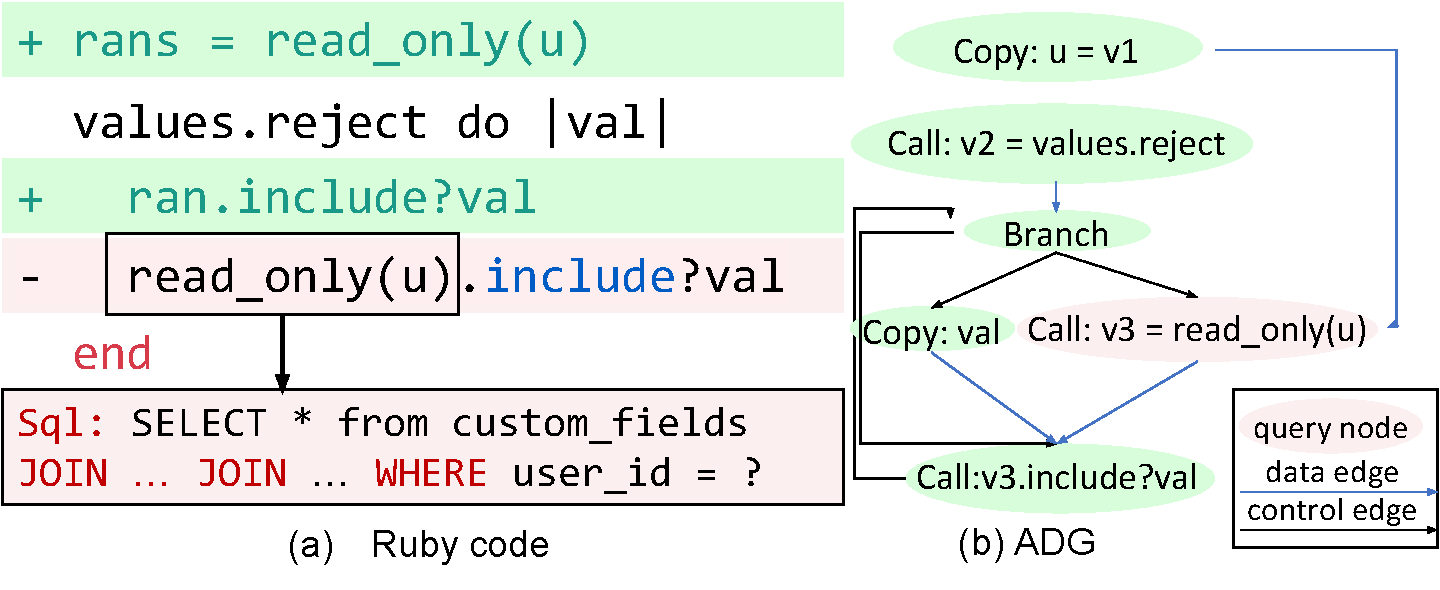
\includegraphics[width=0.8\columnwidth]{figs/redCom.pdf}

  \caption{Loop invariant query from Redmine \textmd{(the code checks which {\tt val} in {\tt values} 
  list belongs to user {\tt u}'s read-only fields})
  %\shan{the patch seems wrong}
  }
\label{fig:loopinv}
\end{figure}



\textbf{Dead store queries (DS)~\cite{junwen:icse2018}.} SQL queries are repeatedly issued to assign the same
memory object with different database contents, without any use of the memory object in between, making all but the last query unnecessary.

\textbf{Unused data-retrieval queries (RD)~\cite{chen2016finding, junwen:icse2018}.} 
Data is retrieved from the database but never 
used in the program, making the corresponding data transfer and query execution unnecessary. 

\textbf{Common sub-expression queries (CS) \cite{yan:cikm17}.} Queries with common sub-expressions are issued, causing 
unnecessary re-computation.

\textbf{API misuses (IA) \cite{junwen:icse2018}.} Different ORM APIs retrieve the same contents from the database, but they differ drastically in terms of performance.
%Our previous work \cite{junwen:icse2018}
%identified 9 such simple ORM-API misuses that do not affect functionality but hurt performance greatly. 
For example, the two Rails code snippets in Figure~\ref{fig:spreeAny} both check if a {\tt user} owns
any blog posts. However, they use different APIs, {\tt count} versus {\tt exist}, that are translated to different
SQL queries by Rails: {\tt select count} vs. {\tt select limit 1}.
The former query scans all records in the {\tt blogs} table with specified {\tt user\_id}, counts the number of records, and checks (in the Ruby application) if the count is greater than 0.
%\shan{all records or all records with specified id?} \junwen{with specified user\_id}
The latter query
returns immediately when it finds one record with the specific {\tt user\_id}, 
which can reduce query execution time by 1.7$\times$ comparing to the former.
%The latter can easily improve the resulting application performance by %1.7$\times$~\cite{junwen:icse2018}. 
%about half a second latency difference in real-world social network applications 

\begin{figure}
\centering
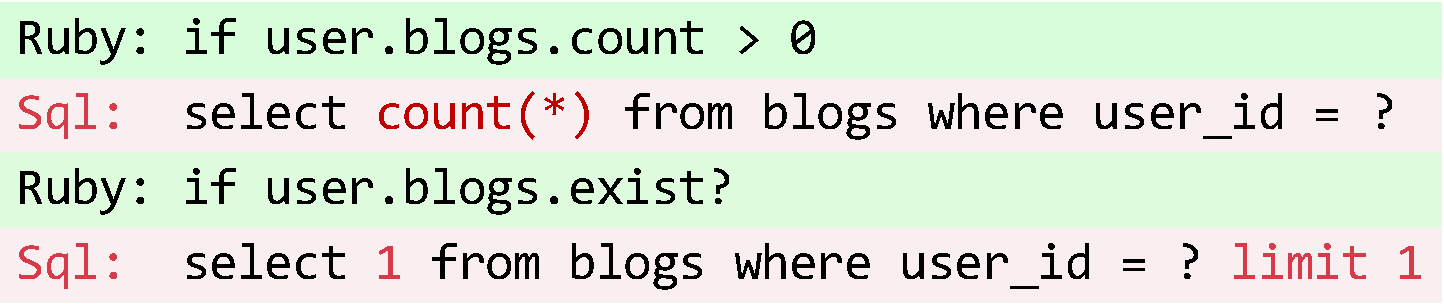
\includegraphics[width=0.6\columnwidth]{figs/api.pdf}
  
\caption{API misuse from Onebody \textmd{(the upper code is less efficient than the lower code)} %\shan{Why {\tt user\_id =1}}
}
 
\label{fig:spreeAny}
\vspace{-0.2in}
\end{figure}

\textbf{Inefficient data rendering (IR) \cite{junwen:icse2018}.} While rendering a list of objects, helper
functions are often used to render a partial view for one object at a time, with much redundant
computation repeated for every object. For example, the HTML in 
Figure \ref{fig:rendering}b is generated line by line by repeated invocations of {\tt link\_to}
with much redundancy across lines. Such inefficiency is particularly severe when there are 
many objects to render. Consequently, it could become a scalability bottleneck when
the objects need to be first retrieved from database. 
%\alvin{why this only happens after  objects are returned by db}

We find these six anti-patterns to be prevalent even in well-developed applications as 
developers are often unaware of what database
queries are issued due to the ORM abstraction. Such queries also cannot be
optimized by traditional Ruby compilers as they treat ORM APIs as
black boxes (nor database engines as they can only observe the queries issued by the application). We next explain how \Tool can detect such patterns.


%Figure~\ref{fig:sub} shows an example of statements which will issue queries that share common subexpressions. The common subexpression among two statements is \textit{projects.visible.order('id ASC')}. By caching it firstly, a better performance can be achieved. In order to detect this inefficiency, we should check whether the same query function is used in two different query function chains. If so, the corresponding queries share a common subexpression. After knowing which subexpression has been shared, we can cache the shared subexpression firstly by creating a new variable and replace the later usage of the subexpression with the new variable. We will also ensure there is no name conflict to make sure the program correctness.

%\begin{figure}[H]
%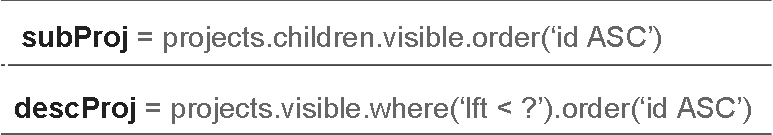
\includegraphics[width=\columnwidth]{figs/sub.pdf}
%\caption{queries share common subexpressions}
%\label{fig:sub}
%\end{figure}


\begin{comment}

\begin{table}[t]
\centering
\caption{Performance anti-patterns}
\vspace{-0.1in}
{\small
\label{tab:perfhis}
\begin{tabular}{lc@{\hspace{4pt}}c@{\hspace{4pt}}c@{\hspace{4pt}}c@{\hspace{4pt}}c@{\hspace{4pt}}c@{\hspace{4pt}}c@{\hspace{4pt}}c@{\hspace{4pt}}c@{\hspace{4pt}}c@{\hspace{4pt}}c@{\hspace{4pt}}c@{\hspace{4pt}}}
\toprule
   &\multicolumn{6}{c}{Auto-Detection} & \multicolumn{6}{c}{Auto-Fixing}\\
   \cmidrule(lr){2-7}
   \cmidrule(lr){8-13}
   & LI & DS & RD & CS & IA & IR & LI & DS & RD & CS & IA & IR    \\
\midrule
FRDA \cite{chen2016finding}& & & \cmark &&&& & & &&&&\\ 
\cite{yan:cikm17}     & & &  &\cmark&&& & & &&&&\\
\cite{junwen:icse2018}& & &  &&\cmark&& & & &&&&\\
\small{\Tool}  &\cmark&\cmark&\cmark&\cmark&\cmark&\cmark&\cmark&\cmark&\cmark&\cmark&\cmark&\cmark\\
%Loop Invariants   &  API checker\cite{junwen:icse2018} & PowerStation & PowerStation   \\
%Dead Stores   &  API checker\cite{junwen:icse2018} &PowerStation & PowerStation   \\
%Unused Data  &  FRDA\cite{chen2016finding} & FRDA\cite{chen2016finding}  & PowerStation   \\
%Common Sub-expr & AFG\cite{yan:cikm17} & AFG \cite{yan:cikm17} & N/A  \\
%API Misuses   & API checker\cite{junwen:icse2018} & API checker\cite{junwen:icse2018}  & PowerStation  \\
%Inefficient Render  &  API checker\cite{junwen:icse2018} & PowerStation  & PowerStation   \\
\bottomrule
\end{tabular}
}
\vspace{-0.1in}
\end{table}
\end{comment}


\section{\Tool's static analysis}
\label{sec:impl}
\Tool's static analysis contains two components. The first takes in Rails source code and generates
a database-aware program dependency graph for every action,\footnote{An action is a member method of a
Ruby controller class. When a web application receives a request, a corresponding action will execute to respond to the request.}
which we refer to as the action
dependency graph (ADG). The second component takes in the ADG, identifies
performance anti-patterns, and synthesizes fixes. We anticipate extending \Tool to tackle other ORM-related performance issues in the future.


%\shan{1.should put much more details here. I have no idea how your tool is implemented. You should save space from describing patterns and put more text here; 2. you didn't explain how fix-suggestion is generated}

\subsection{Database-aware Static Analysis Framework} 
\Tool's static analysis framework goes through the following steps to generate ADG from Ruby on Rails source code.

\textbf{Pre-processing.} \Tool performs inter-procedural analysis on the source code by statically inlining all function calls. It also inlines callbacks such as {\tt ActiveRecord} validations invoked by this action. Since Ruby is dynamically typed, \Tool performs type inference~\cite{furr2009static} to statically determine variable types.

%\Tool first inlines function calls to enable inter-procedural analysis. This
%process involves type inference~\cite{furr2009static}, as Ruby is dynamically typed, 
%and identifying Ruby code that is implicitly
%invoked by an controller action through view rendering, 
%Rails callback functions, {\tt ActiveRecord} validation functions, etc. 

%\alvin{too much detail?}


\textbf{Program dependency graph (PDG) generation.}
\Tool generates a PDG for every controller action, which is the entry function that eventually produces a webpage.   
It uses JRuby 
%\cite{jruby} 
to parse the pre-processed source code, and then builds the PDG from JRuby's intermediate
representation (IR) as this IR nicely captures high-level Ruby semantics via instructions and operands.
As illustrated in Figure \ref{fig:loopinv}b, every node $n$ in the PDG represents a statement in the JRuby IR. 
%and
%is of the type, Assign, Call, Branch, Const, Copy, HashField, ReceiveArg, or
%Return. 
%Related information like source code location and variable names are also kept. 
Every edge $e$ in PDG represents either control dependency or data dependency.
A data-dependency
edge $n_1 \rightarrow n_2$ indicates that the output object $o$ of $n_1$ is used by $n_2$ without
other statements overwriting $o$ in between.

\textbf{Database-aware ADG Generation.}
\Tool then enhances the PDG generated above in three ways to create the ADG: 
(1) changing and splitting some nodes to become 
Query nodes; (2) annotating every Query node with the database table and fields that are read or written; 
(3) annotating every outgoing data-dependency edge of a Query node with the exact field(s) that are used.

To accomplish this, \Tool first analyzes every model class that extends the Rails
{\tt ActiveRecord} interface to determine all the database
tables in the application and the association relationship among them.
For example, analyzing the model classes illustrated in 
Figure~\ref{fig:schema}, \Tool identifies the {\tt users} table
corresponding to the {\tt User} class and similarly for the {\tt Blog} class, and that these two models have 
a one-to-many relationship, i.e., each instance of {\tt User} may own multiple instances of {\tt Blog}.
Second, \Tool analyzes the {\tt schema.rb} file to determine
how many fields each table contains. For example, parsing the
{\tt schema.rb} snippet in Figure~\ref{fig:schema}, \Tool infers the schemas of the {\tt users} and {\tt blogs} tables as
shown in the bottom of the figure.

Third, \Tool identifies queries from three sources: (1) explicit 
invocations of
Rails {\tt ActiveRecord} Query APIs, such as {\tt exist?},
{\tt reload}, {\tt update}, {\tt destroy}, etc;
(2) implicit queries generated by Rails to access object fields, e.g., {\tt $o_1$.$o_2$}, where 
the class of $o_1$ and the class of $o_2$ are associated model classes
(e.g., {\tt user.blogs} would incur a query to
retrieve records in {\tt blogs} table that are associated with
the specific {\tt user} record in {\tt users} table);
(3) embedded SQL queries through {\tt Base.connection.execute}.
%\junwen{it's also thru the ActiveRecord API, similar as the first type}
Any query identified above is represented as a Query node in the ADG.\footnote{At run time,
multiple such queries could be composed by ORM into one SQL query.
Such query chaining does not affect \Tool's analysis.} 
%\alvin{still think that there is too much detail here}
%\junwen{schema helps us differentiate between the fields and the associations, if it only retrieves certain field, then it will not issue a query, but if it retrieve the association, then it will issue a query}


\begin{figure}
    \centering
    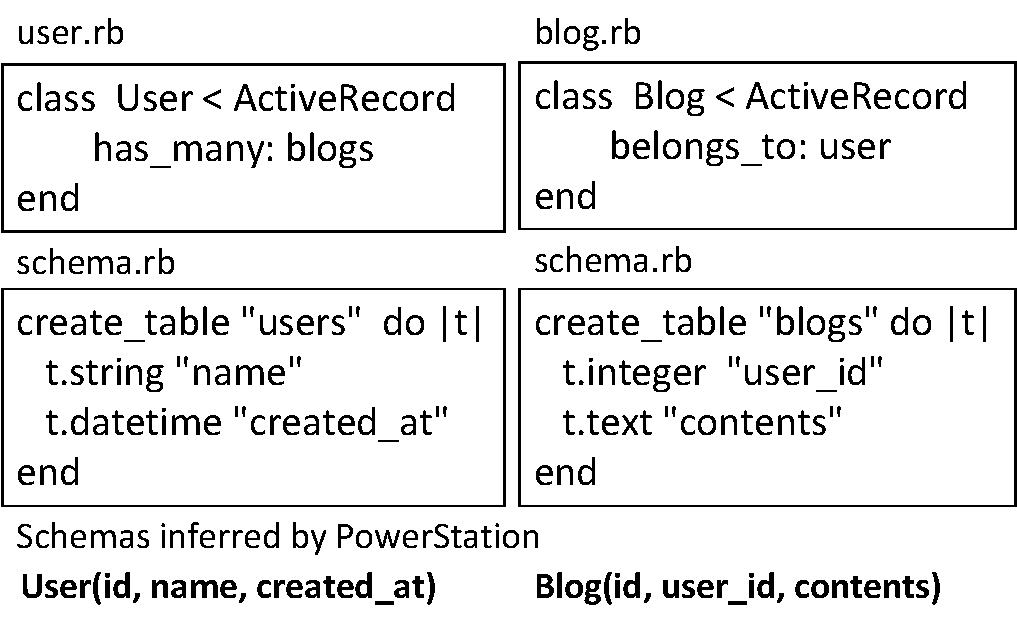
\includegraphics[width=0.7\columnwidth]{figs/schema.pdf}
    \caption{Analyzing table schemas}
    \label{fig:schema}
\end{figure}

\iffalse
\textbf{Final ADG output.} It  is the same as the traditional PDG. Given an action, the ADG of it g is represented as a four-tuple element, g = (V, E, $\mu$, $\delta$), in which, 

\begin{itemize}
\item V contains the vertex which represents the program statement in the action including the involved variables. Moreover, each vertex also contains the corresponding location in the source code including the filename and the line number. 

\item E is the set of edges which represent the dependency between vertices.

\item $\mu$ assigns Assign, Call, Branch, Const, Copy, HashField, ReceiveArg, or Return types to vertices. 

\item $\delta$ assigns whether a edge is Control or Data.
\end{itemize}
Given a source vertex v$_s$, and a target vertex v$_t$, if  v$_s$ is a Branch, and its truth controls
the execution of  v$_t$, then the edge between v$_s$ and v$_t$ is a Control edge. If v$_t$ reads the variable assigns in v$_s$ and there is a execution path between v$_s$ and v$_t$, then the edge is a Data edge.
\fi

\subsection{Detecting and Fixing Anti-patterns}
\textbf{Loop invariant queries.} \Tool first identifies all query nodes inside loop bodies in ADG. For each such node $n$, 
it checks the incoming data-dependency edges of $n$. If all of these edges start from outside the loop $L$
where $n$ is located, then $n$ is identified as a loop-invariant query, such as ``Call: v3...'' in Figure \ref{fig:loopinv}b.
%The analysis will output the query statement as well as the filename and line number as the location information, and  the location of the start of the loop. %If this statement has not been assigned to the local variable inside the loop, we will also generate a variable name  randomly in order to avoid the name conflict with other variables. 
To fix this, \Tool inserts a new Assign statement before the start of the loop, where a newly created variable $v$
gets the return value of the loop-invariant query, and replaces every invocation of the loop-invariant query inside loop $L$
with $v$.

\textbf{Dead store queries.}  \Tool checks every ADG node that issues a reload query, i.e., {\tt o.reload}, %\alvin{does it have to assign to the same object?} 
and checks its out-going data-dependency
edge. If there is no such edge, i.e., the reloaded content is not used, then the query is marked as a dead-store query that is deleted by \Tool.
%To synthesize a fix, \Tool simply deletes the reload statement.

\textbf{Unused data retrieval queries.} For every Read query node $n$ in the ADG, \Tool first computes the database fields loaded by $n$ that are used subsequently. This is the union of
the \textit{used fields} associated with every out-going data-dependency edge of $n$. 
\Tool then checks if every loaded field is used. For every unused field,
\Tool either deletes $n$, if none of the fields retrieved by $n$ are used, or adds field
selection {\tt .select(:f1, :f2, \ldots)} to the original query in $n$ so that only used fields
{\tt f1}, {\tt f2} are loaded. 


\textbf{Common sub-expression queries.} \Tool checks every query node $q_0$
in ADG to see if $q_0$ has out-going data-dependency edges
to at least two query nodes $q_1$ and $q_2$ in the same control path. If that is the case, then
by default, Rails would issue at least two SQL queries that
share common sub-expression $q_0$ at 
run time, one composing $q_0$ and $q_1$ and one composing 
$q_0$ and $q_2$,
%\shan{Don't you need to check if $q_1$ and $q_2$ might appear in one control path?}
with the latter unnecessarily evaluates $q_0$ again.
%As mentioned, query components are composed through call chains \cong{make sure it is discussed}. It is often seen that a partial chain diverges into multiple chains later, as a result, the component in the partial chain is shared by different queries. For example, {\tt u=user.where(:age>21)} is a partial chain that selects users over 21 years old. The application later gets the count of such users and a list of blogs written by them by calling {\tt u.count} and {\tt u.blogs}, which correspond to a {\tt COUNT} query and a {\tt JOIN} query. These two queries share the same subexpression {\tt `WHERE age>21`}. Powerstation finds common subexpression by discovering the above pattern: if a partial call chain contains any query vertex, and is later diverged into multiple chains where multiple queries are issued, then these queries share common subexpression.\shan{???}
This can be optimized by changing the query plan and caching the common intermediate result for reuse~\cite{yan:cikm17}. 
Doing so requires issuing raw SQL commands that are currently not supported
by Rails {\tt ActiveRecord} APIs. 
%Since such fix might hurt code readability, the current prototype of \Tool does not automatically
%generate such fixes. \alvin{is the current goal of \Tool to generate `human readable' code? I see \Tool as a compiler like gcc and hence does it matter how ugly the generated code looks like?} \junwen{PowerStation now makes change on source code, so the goal is to generate human readable code}

%We chain the query vertex in ADG through the data edge and check whether the same query function is used in two different query function chains\shan{Don't understand this sentence}. If so, the corresponding queries share a common subexpression\shan{Don't understand. What is the common sub-expression?}.
%Fixing this problem requires operation to the database such as creating a template, unfortunately, Rails doesn't provide such API for us to automatically solve it in the source code\shan{Doesn't Ruby allows you to embed raw SQL command in program? Why cannot you do that?}.

\textbf{API Misuses.} 
\Tool uses regular expression matching to find inefficient API misuses as in previous work~\cite{junwen:icse2018}.
%\shan{Do you do this on ADG or not? Your current description does not sound like so}. \junwen{both are implemented, since regex is easier to describe, so I chose it.}
Since these API mis-use patterns are simple, \Tool also synthesizes patches for each API mis-use pattern through regular expressions. %\alvin{do all misues only involve one function call as in the case of `count'? If not what if instead of writing o.f1.f2 they wrote v = o.f1; v.f2 ?}


\textbf{Inefficient rendering.} \Tool checks every loop in the ADG to see if it iterates through objects returned by queries and contains a Rails view helper function 
such as {\tt link\_to} in every loop iteration.
If so, \Tool identifies the code as having the inefficient rendering
problem. To fix this, \Tool  
%\alvin{why suggest? does it not do it automatically?} 
hoists the helper function out of the loop, assigns its result to a newly created variable, and replaces the original
helper function in the loop with {\tt gsub} (a string substitution function) on the newly created variable, as shown in Figure \ref{fig:rendering}. Doing so removes the redundant rendering that is performed on every loop iteration in the original code.

\begin{figure}
    \centering
    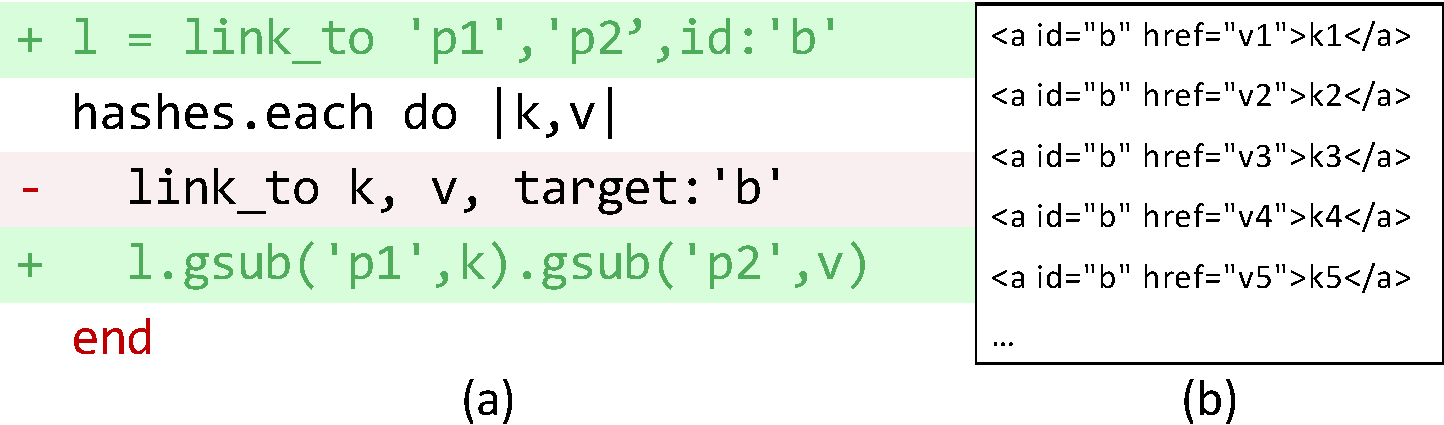
\includegraphics[width=0.7\columnwidth]{figs/rendering.pdf}
% \vspace{-0.1in}
    \caption{Fix for inefficient rendering %{\tt content\_tag (:div, value} creates a xxxx)
    \textmd{({\tt gsub} is a string substitution API, replacing its first parameter with the second)}
    }
    \label{fig:rendering}
%    \small{The {\tt content\_tag(:div, value)} will create a div tag as {\tt <div>value</div>}.}

\end{figure}

\textbf{Discussion.}
%\Tool static analysis could report false positives. Because the analysis is targeted on single action. 
Like other code refactoring tools, \Tool currently suggests fixes to the user rather than deploying them automatically. This is important for Dead Store and Unused Data cases, since the \Tool-suggested fixes would change application semantics if the retrieved data is used in multiple actions.
%make \Tool fixes invalid---developers can check before accepting \Tool fixes. 
For the other cases, however, \Tool's suggested fixes do preserve program semantics.

\section{\Tool IDE integration}
\label{sec:ui}

\subsection{\Tool IDE Plugin Features}
We have implemented \Tool as an IDE plugin for RubyMine \cite{RubyMine}, a popular IDE
for Ruby on Rails. A screenshot of \Tool is shown in 
Figure~\ref{fig:pw}. By pressing the ``PowerStation'' button 
at the top of RubyMine, users can choose an analysis scope, 
``Whole Application'' or ``Single Action,''
and launch \Tool analysis accordingly. 
%``Whole Application'' starts \Tool by performing static analysis on the loaded application code. ``Single Action'' allows users to choose a single action and performs analysis on its source code. 
Our website includes a tutorial~\cite{powerstation}.

\textbf{Issues list.} The right panel, as highlighted in Figure \ref{fig:pw}, lists all the
inefficiencies detected by \Tool, each represented by a button displaying the file where
the inefficiency is located. 
By default, all the inefficiencies found in the project are listed. %\shan{right?}.
Users can also choose to display inefficiencies of a particularly type as shown in Figure \ref{fig:pw}---loop invariant queries (LI), dead store queries (DS), unused data retrieval queries (RD), 
common sub-expression queries (CS), API misuses (IA), and inefficient rendering (IR).

\textbf{Issues highlight.} 
Clicking the file button in the issue list will navigate users 
to the corresponding file in the editor, with the inefficient code 
highlighted. Hovering the cursor over the highlighted code will display the reason for highlighting, as shown in Figure~\ref{fig:pw}.
%, it shows that under the dead-store query anti-pattern category, there is one file named \textit{blogs\_controller.rb}, and the left editor highlights line 33, and line 34 which involves the dead store queries. 

\textbf{Issue fix.} Clicking the ``fix'' button next to each issue in the issue list will 
pop up window asking the user whether she wants \Tool to fix the issue. If so, \Tool will synthesize a fix as discussed in 
Section~\ref{sec:impl}, and display the fixed code in the editor panel. 
At that point, the original ``fix'' button becomes an ``undo'' button, allowing users to revert the fix if needed.

\begin{figure}
\centering
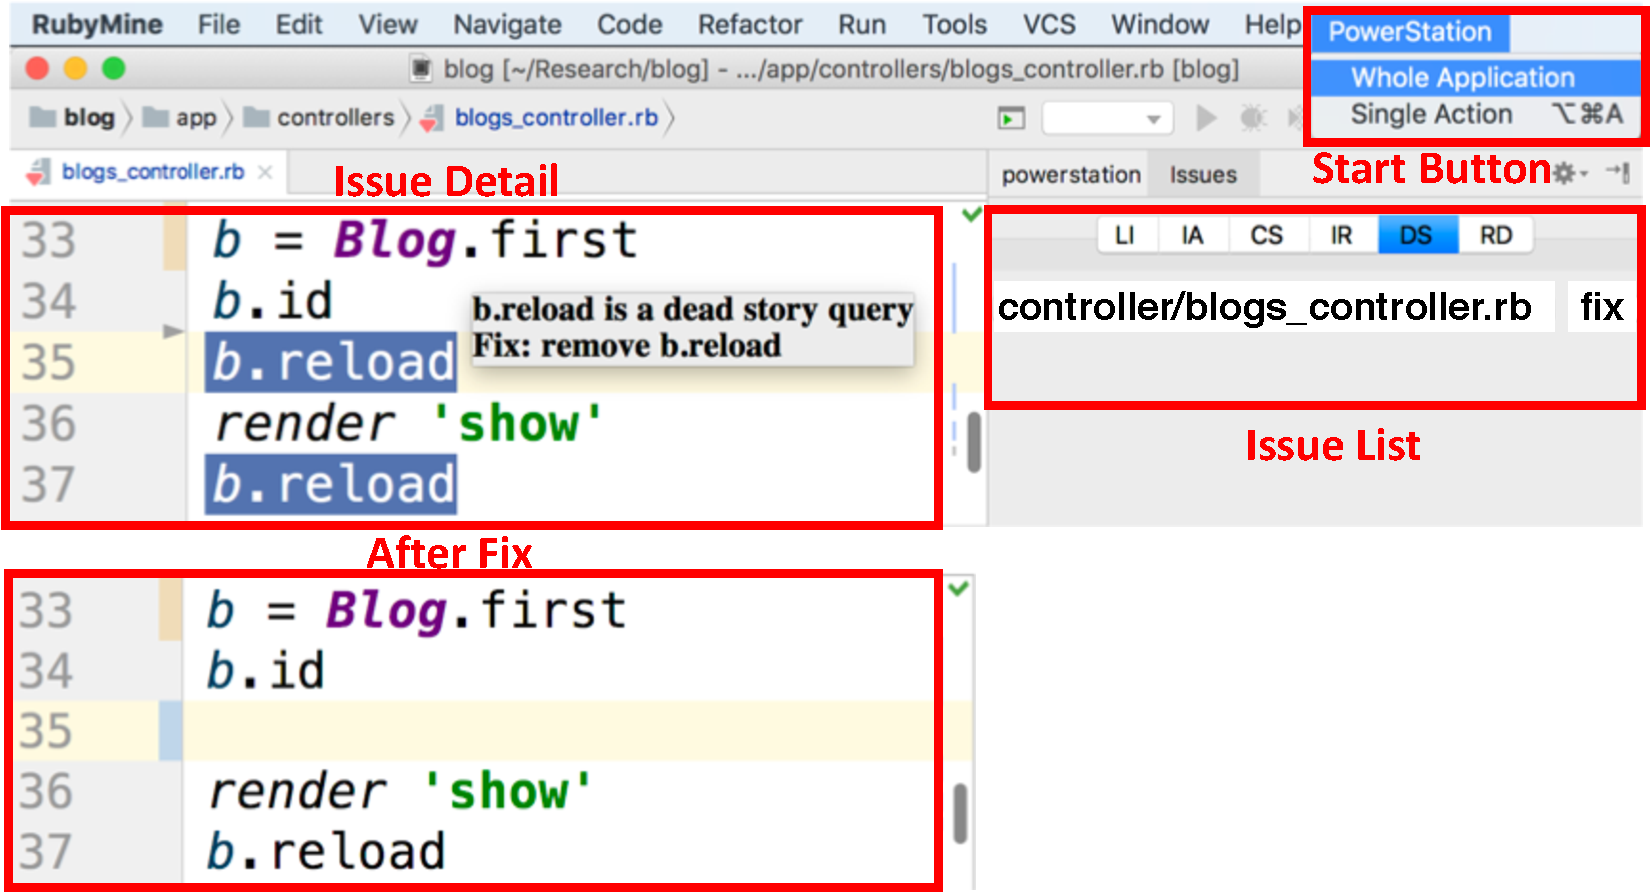
\includegraphics[width=0.9\columnwidth]{figs/after.pdf}
\vspace{-0.1in}
\caption{Screenshots of \Tool IDE Plugin}
\label{fig:pw}

\vspace{-0.25in}
\end{figure}

% \begin{figure}
% \centering
% 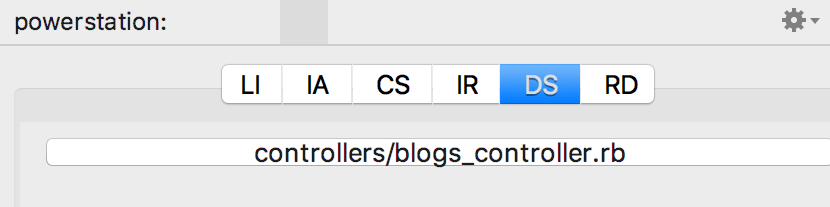
\includegraphics[width=\columnwidth]{figs/issue-list}
% \vspace{-0.1in}
% \caption{Issue list of PowerStation%\shan{this figure is really wasting space. we should have such snapshots but need to contain much more information\ than this. maybe multiple shots are better?}
% }

% \label{fig:issue-list}
% \end{figure}
\begin{comment}

\begin{figure}[t!]
%\centering
%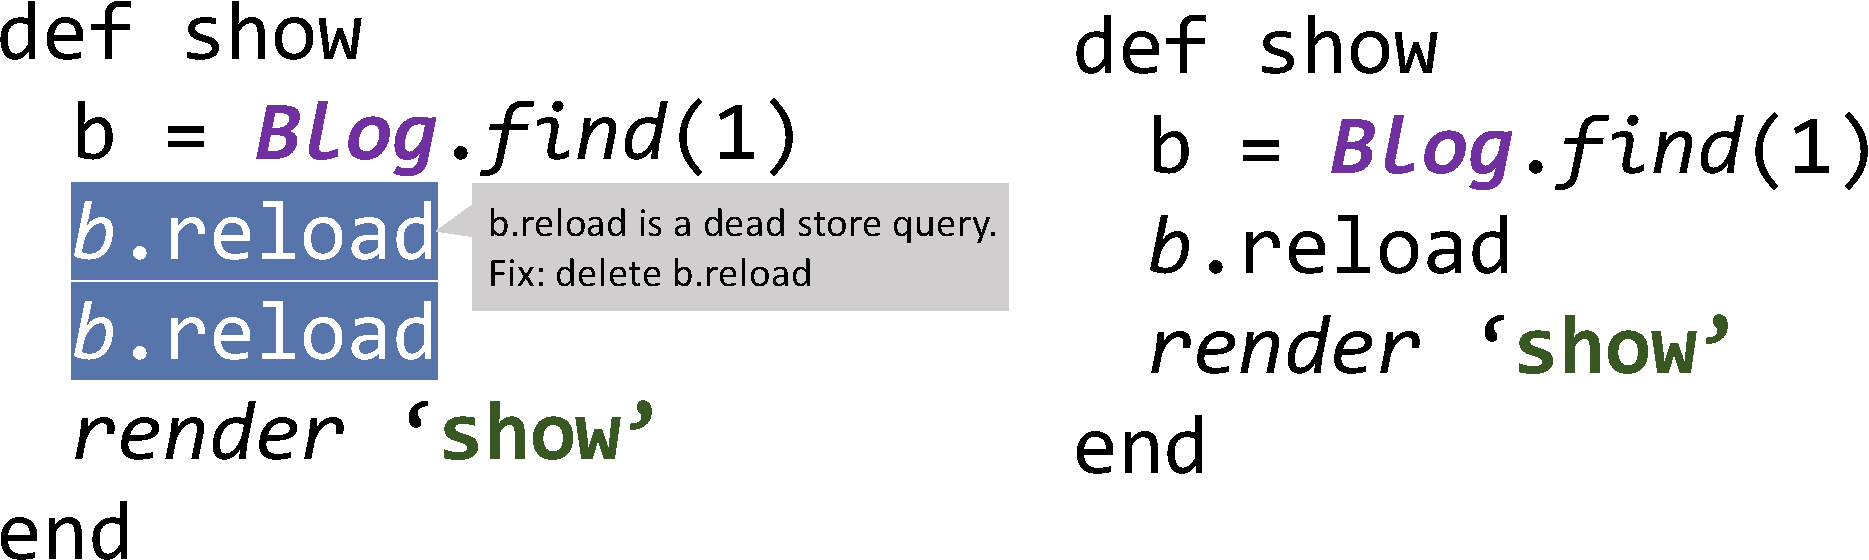
\includegraphics[width=\columnwidth]{figs/issue-detail}
\begin{subfigure}[t]{0.5\textwidth}
        \centering
        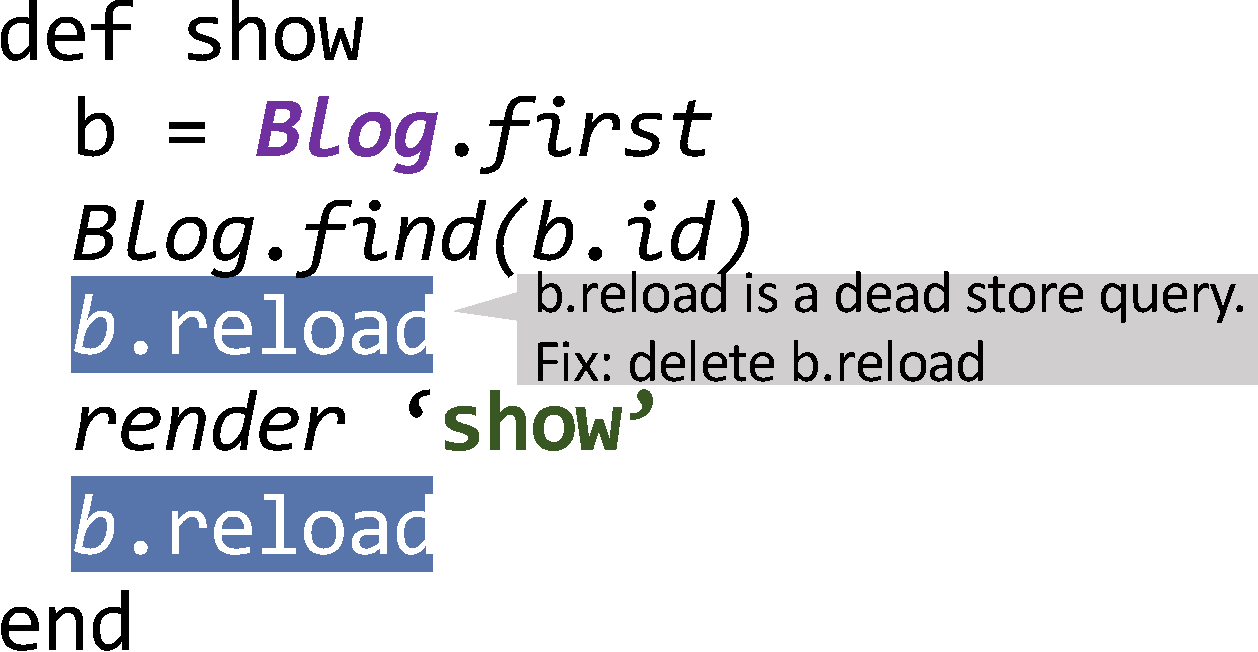
\includegraphics[width=0.45\columnwidth]{figs/before.pdf}
        \caption{Before fix}
        \label{fig:bfix}
 \end{subfigure}%
 \begin{subfigure}[t]{0.5\textwidth}
        \centering
        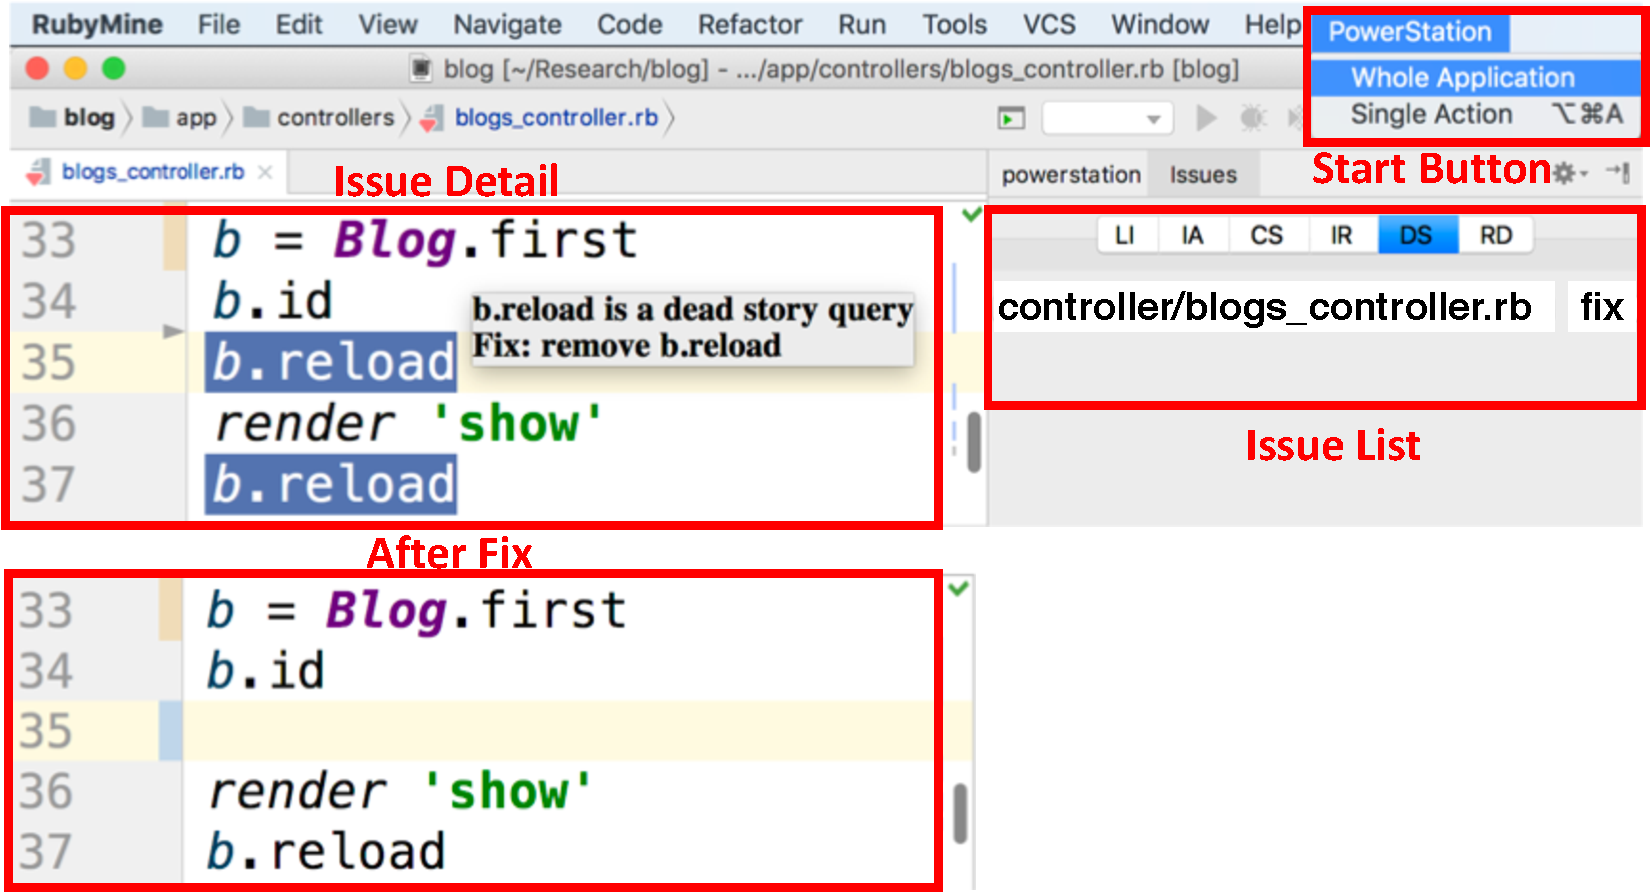
\includegraphics[width=0.45\columnwidth]{figs/after.pdf}
        \caption{After fix}
        \label{fig:afix}
 \end{subfigure}%
\vspace{-0.1in}
\caption{Issue details in Editor \shan{Very strange figures. 1. The code on the left is 
different from the code in Figure 6; 2. It is unclear what is the relationship between
the left side and the right side; } }
\label{fig:ide}
\end{figure}

\end{comment}

\vspace{-2mm}
\subsection{Implementation}

We used the APIs provided by the
IntelliJ Platform like {\tt ToolWindow} and
%~\cite{toolwindow} and 
{\tt JBTabbedPane}
%~\cite{guidesigner} 
to create the \Tool issues list.

Highlighting the selected inefficiency is straight-forward using
the IntelliJ API {\tt HighlighterLayer}, given file name and line number provided by \Tool static analysis.

For every anti-pattern, \Tool prepares a string template that explains the inefficiency and the fix strategy,
such as ``* is a dead store query. Fix: delete *.'' for a dead-store query (Figure \ref{fig:pw}). This string
is instantiated with program variables and expressions output from \Tool static analysis, and displayed using
the IntelliJ API {\tt FileDocumentManager}.

Finally, IntelliJ API {\tt FileEditorManager}, {\tt TextRange}, and {\tt Document} are used to insert, replace, and delete source code
in the editor panel. 
%Table~\ref{tab:fixop} shows the fix operation needed for different anti-patterns.

\iffalse
\begin{table}[H]
    \centering
    \begin{tabular}{c|c}
    \toprule
         API Misuse  & replacement \\ 
        Loop Invariant Query &  insertion and replacement\\ Dead-store Query  &  deletion\\ 
        Unnecessary Data Retrieval  & deletion or replacement\\
         Inefficient Rendering &insertion and replacement \\
         \bottomrule
    \end{tabular}
    \caption{Fix Operation}
    \label{tab:fixop}
\end{table}
\fi
%The IntelliJ Platform provides all of the infrastructure which IDEs need to provide rich language tooling support. It has a component driven, cross platform JVM based application host with a high level user interface toolkit. By using it we are able to create tool windows which will be used to show the performance issue list, and we can create popup menus  used to show the details of the performance issues and the fix suggestions. Moreover, it also includes a full text editor, and provides abstract implementations of syntax highlighting, code folding, code completion, which we use to highlight the code involving in the anti-patterns. Also, Program Structure Interface (PSI) enables  quick navigating to files which allows us to open the specified files which contain the performance issues source code. Also, code inspections and code rewriting provided by PSI gives us opportunity to do quick fixes or refactorings.

%IntelliJ is a platform for building multi-language IDE's and plugins, and includes components such as UI elements, a text editor, frameworks for code manipulation, including code navigation and inspection, and plugin development APIs.  It also supports code execution and debugging.


%The main APIs that were used from the Intellij Platform in implementing Powerstation include the IntelliJ plugin development API and Java's Swing and AWT APIs.  The IntelliJ plugin development API was used for operations that use the source code of the inputted project or change properties of the IDE.  In particular, it was used to read and write source code (e.g. string-matching and replacing inefficient API uses), navigate to specific files which contain the source code for performance issues, highlight code, and embed the Powerstation plugin into the IDE by adding an IDE menu option for it. Java's Swing and AWT APIs were used to create visual components of Powerstation's user interface (UI).  In particular, they were used to create a side window giving the user a choice of the issue they want to fix, a tool window that displays a list of performance issues, a checkbox that displays the performance issues by category, file name, and line number, and a pop-up menu with fix suggestions.



\section{Evaluation}

\label{sec:evaluation}

%\shan{1. don't call this ``performance evaluation''. ``Performance'' usually
%means how long it runs.
%2. please don't put a column that shows 0; 3. need to explain the applications briefly; 4. i see many tool paper shows ``case studies''.
%that should be included either here or earlier}

\Tool can be downloaded from IntelliJ plugin repository \cite{downloadPW} %\shan{what is the downloading URL?} 
and easily installed in RubyMine. 
%by  selecting "Install plugin from disk" in RubyMine. 
%There is a compiled JRuby pacakage should be downloaded together in order that PowerStation can establish static analysis based on  dataflow log generated by JRuby.  
%After that, developers can simply start using PowerStation by clicking the analyze and show button on the RubyMine menu.  

We evaluated \Tool using the latest versions of 12 open-source 
Rails applications, including the top two popular applications on Github from 6 categories: Forum, Collaboration, E-commerce, Task-management, Social Network, and Map.
As shown in Table~\ref{tab:perfbug}, \Tool can automatically identify \issueNum inefficiency issues and generate patches for \fixedIssueNum of them (i.e., all but the common sub-expression pattern). We randomly 
sampled and examined half of the reported issues and the suggested fixes,
and found no false positives. %\shan{yes or no?}. 
Due to the limited resource and time, we reported 
\reportedIssue issues with \confirmedIssue of them already confirmed by developers (none
has been denied). 
\Tool static analysis is fast, taking only 12--625 seconds to analyze the entire application
that ranges from 4k to 145k lines of code in our experiments on a Chameleon instance with 128GB RAM and 2 CPUs. 
%This analysis can be done in background while developers working on other projects in the IDE. 
Developers can also choose to analyze one action at a time, which usually takes less than 10 seconds 
in our experiments.
%4663 to 145351 lines of code \shan{How can it be interactive???}.

\begin{table}
\centering
\caption{Inefficiencies detected by \Tool in 12 apps}
% \vspace{-0.15in}
{\small
\label{tab:perfbug}
%\resizebox{0.6\columnwidth}{!}{%
\begin{tabular}{lrrrrrrr}
%{p{0.4cm}R{1cm}R{1cm}R{1.2cm}R{1cm}R{1cm}R{0.8cm}}													
\toprule													
App.	&	Loop   Invariants	&	Unuse  Data	&	Common  Sub-expr	&	API   Misuses	&	Inefficient Render	&	SUM	\\
\midrule													
Ds	&	0	&	16	&	106	&	85	&	0	&	207	\\
\midrule													
Lo	&	0	&	2	&	0	&	45	&	5	&	52	\\
\midrule													
Gi	&	0	&	14	&	92	&	23	&	1	&	130	\\
\midrule													
Re	&	0	&	11	&	101	&	59	&	0	&	171	\\
\midrule													
Sp	&	0	&	22	&	0	&	20	&	0	&	42	\\
\midrule													
Ro	&	0	&	3	&	0	&	11	&	0	&	14	\\
\midrule													
Fu	&	0	&	12	&	15	&	2	&	1	&	30	\\
\midrule													
Tr	&	0	&	23	&	30	&	30	&	1	&	84	\\
\midrule													
Da	&	1	&	55	&	36	&	57	&	0	&	149	\\
\midrule													
On	&	0	&	17	&	39	&	76	&	0	&	132	\\
\midrule													
FF	&	0	&	24	&	12	&	4	&	5	&	45	\\
\midrule													
OS	&	0	&	89	&	60	&	16	&	0	&	165	\\
\midrule													
SUM	&	1	&	288	&	491	&	428	&	13	&	1221	\\					
\bottomrule															
\end{tabular}
%}
}
\end{table}


\vspace{-2mm}
\section{Conclusion and Future Work}
\Tool is a new tool that automatically detects and fixes a large set of 
ORM-related performance issues that are both common and severe in database-backed
web applications. Its integration with RubyMine provides an easy way for
Rails developers to avoid making performance-degrading mistakes in their
programs. We have used \Tool to identify and fix many performance-related issues in real-world applications, and will extend \Tool tackle further performance anti-patterns as future work.

% \vspace{-2mm}
% \section*{Acknowledgements}
% This work is supported in part by the National Science Foundation through grants IIS-1546083, IIS-1651489, IIS-1546543, OAC-1739419, CNS-1514256, CCF-1514189, and CNS-1563788; DARPA award FA8750-16-2-0032; DOE award DE-SC0016260; gifts from Adobe, Google, and the CERES Center for Unstoppable Computing.

\chapter{Panorama: View-Centric Performance Optimization}


% \section{Motivating Examples}
% \input{motivate}

%\section{Approach}
%
\label{sec:app}
%\subsection{Overview}
Figure~\ref{fig:app} shows the overview of our approach.
For each HTML element rendered on the webpage, we calculate the performance cost on it including the wall-clock real-time cost and relative cost towards the database size. This performance information will be displayed on the webpage after it's loaded inside the Browser. And then, for each HTML element, we provide the possible design opportunities. Once developers choose one design opportunity for certain HTML element, the source code will be edited to satisfy the developers' requirement.
\begin{figure}[H]
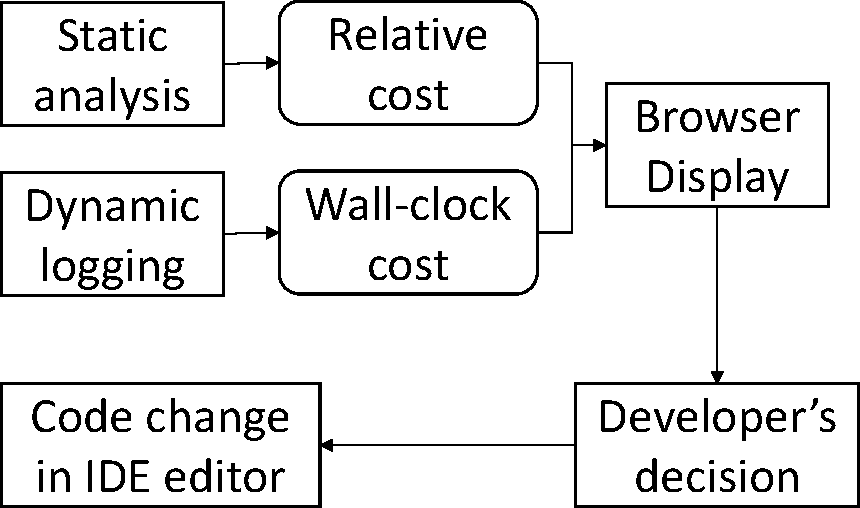
\includegraphics[width=\columnwidth]{figs/p2-crop.pdf}
\caption{Overview of Approach}
\label{fig:app}
\end{figure}
\subsection{Performance Cost Estimation}
We estimates the performance cost for each HTML tag that will be rendered on the page through dynamic run-time logging and static analysis, which is a new granularity for performance estimation. Also our approach includes the wall-clock performance cost and relative performance cost towards the database size. As a result, this approach also works when there is not a representative workload for us to gain enough performance cost information. 
 
\subsection{Interactive Design Interface}
We propose a brand new interface for web application design. We firstly render the performance cost information estimated from last step on the web page for each HTML tag. And for those HTML tags that take large performance cost, we identify the possible alternative design choices from these options: (1) pagination, (2) approximation, (3) asynchronous loading, and (4) removing. Developers are allowed to choose their desired design choice. After developers' selection, source code will be automatically revised so that the application can achieve their wanted behavior. The performance cost of updated application will re-estimated and displayed on the web page in order that the performance improvement can be observed. 




\section{Overview}

In this chapter, we present a framework called \ToolP that provides a view-centric 
and database-aware analysis
for web developers to understand and optimize 
their database-backed web applications. \ToolP currently targets applications  written using the Ruby on Rails framework, and makes three major contributions as illustrated in Figure \ref{fig:overview}.

\ToolP provides a view-centric estimator that helps developers understand the 
data-processing cost behind every HTML tag. 
\ToolP both dynamically monitors database query performance using the test workload, statically estimates data processing complexity independent of any specific workload, and carefully attributes the cost to every HTML tag
through its cross-stack dependency analysis. The details will be presented in 
Section \ref{sec:profile}.

\ToolP provides a view-aware performance optimizer that helps developers carry out
view-changing code refactoring to improve performance. \ToolP suggests a variety
of refactorings that (1) change the manner of content rendering (i.e., pagination or asynchronous loading);
or (2) change the accuracy of the rendered contents (i.e., approximation);
or (3) remove certain web-page contents from rendered contents. Through static program
analysis, \ToolP not only identifies opportunities for applying such refactoring,
but also automatically suggests patches that complete such refactoring,
often involving modifications to multiple files in model, view, and controller components.
We present the details in Section \ref{sec:opt}.

%We estimates the performance cost for each HTML tag that will be rendered on the page through dynamic run-time logging and static analysis, which is a new granularity for performance estimation. Also our approach includes the wall-clock performance cost and relative performance cost towards the database size. As a result, this approach also works when there is not a representative workload for us to gain enough performance cost information. 

\ToolP provides a unique interface for developers to effectively
exploring different web-page designs with different performance-functionality trade-offs.
Instead of separately presenting profiling information and refactoring suggestions, \ToolP integrates them in the web browser---while testing a page of their web applications, the data processing cost for each HTML tag is presented as a heat map in the browser. Developers can right click on each
HTML tag to see the different view-changing options for performance enhancement; they can 
choose any option and immediately see an updated web page with an updated heat map in the browser,
with all code refactoring automatically done by \ToolP in an accompanying Ruby editor.
%Section \ref{sec:im} explains how \ToolP implements this interface through a combination of
%Ruby editor plug-ins, \ToolP performance-debugging JavaScript, and static instrumentation 
%of the web application under development.

%Users can easily explore various types of optimizations 
%before they decide on the most suitable design that gives the 
%best balance between web-page functionality and page-loading performance. 
%\alvin{this paragraph seems to be more of a description of how \ToolP works. I suggest moving this somewhere else and state precisely what is new about the \ToolP interface here instead}

%Secondly, we implement this approach into a prototype on Ruby on Rails framework through Rails libraries and RubyMine IDE plugin. 




\begin{figure}
    \centering
    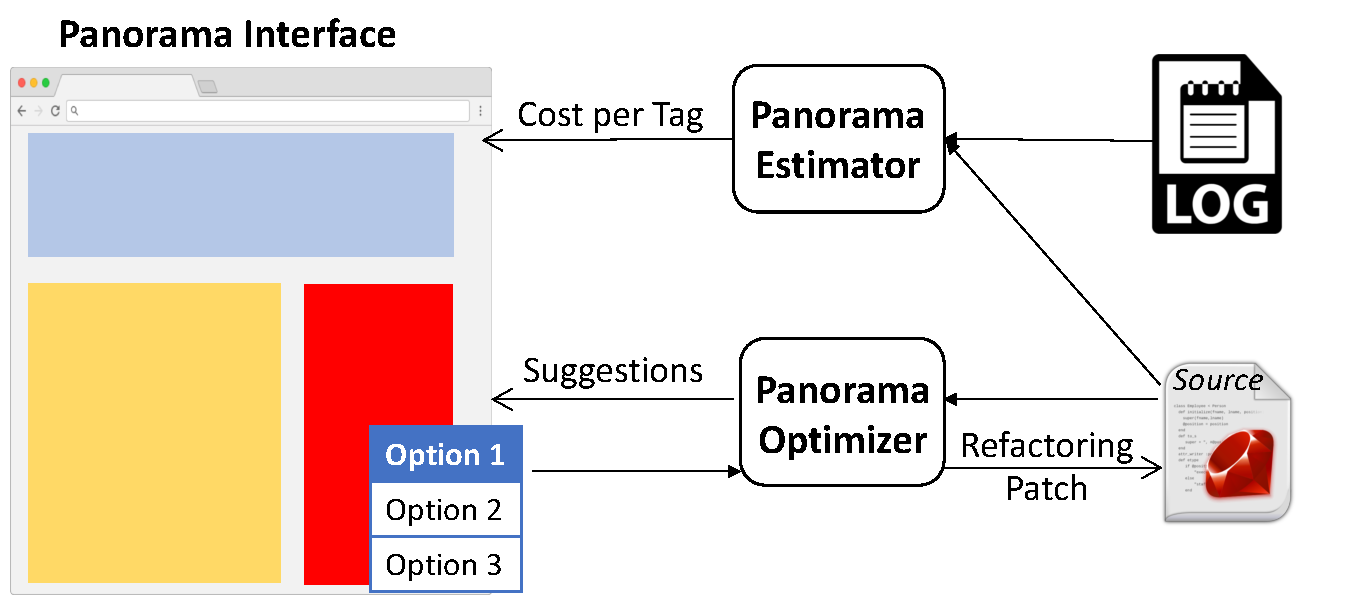
\includegraphics[width=0.7\columnwidth]{panorama-figs/overview.pdf}
    \vspace{-0.1in}
    \caption{\ToolP overview}
     \vspace{-0.2in}
    \label{fig:overview}
\end{figure}


We evaluated \ToolP on 12 popular open-source Ruby on Rails applications.
\ToolP statically identifies \numissues performance-enhancing
opportunities through view changes. We randomly sampled 15 view changes suggested
by \ToolP and found that by applying the patches automatically generated by \Tool,
these 15 view changes speed up end-to-end page load time by \eoespeedup on average
(\maxspeedup maximum), using database workloads that are similar to those used in real-world deployments. We believe the benefits will increase with even larger workloads. %a larger workload will offer even bigger speedup.
Furthermore, we conducted a thorough user study with 100 participants from
Amazon Mechanical Turk. The study shows that web pages with these
view changes are considered as similar or better than the original web pages
in most cases, with more users preferring the design suggested by
\ToolP than the original ones. This user study result, as well as the fact 
that these optimizations save computation resources on web servers and database servers, justify the need for developers to explore the performance-functionality 
trade-off space in web application design, with \ToolP being a first step towards that goal.
\section{Static analysis framework}
\label{sec:frame}

\ToolP leverages a database-aware static analysis framework for 
Rails applications that we briefly describe below.

\subsection{Action dependency graph}
\ToolP's static analysis centers around the
action-dependency graph (ADG) that is constructed for each controller action.
Figure \ref{fig:icq} shows an example of ADG.

%As discussed in previous work \cite{powerstation}, 
An ADG is a database-aware extension 
of the traditional program-dependence graph (PDG)~\cite{ferrante1987program}.
Every node $n$ in the ADG represents an intermediate representation (IR)
statement in the corresponding action's JRuby \cite{jruby} IR.
Every edge $e$
represents either control dependency or data dependency. Edges shown in 
Figure~\ref{fig:icq} all represent data dependencies.

In contrast to the PDG, 
every node in the ADG that issues a SQL query is associated with a query tag in ADG, such as
node {\large \textcircled{\small 1}} and node {\large \textcircled{\small 2}} in Figure~\ref{fig:icq}. 
Information about SQL queries that are issued and the tables they referenced are determined by analyzing  {\tt ActiveRecord} function calls and recorded in the ADG.
%every query that might be issued by an IR statement is split out to be a special query-node in the graph, annotated with database table and fields accessed by the query.
%Furthermore, a data-dependency
%edge $n_1 \rightarrow n_2$ indicates that the output object $o$ of $n_1$ is used by $n_2$ without
%other statements overwriting $o$ in between. For each statement, we keep the line number information. Combining with the APIs provided by ActiveRecord and the database schema information, we further decide whether a node is a query. 
%This information is generated by carefully processing every model class extending the Rails
%{\tt ActiveRecord} interface, the {\tt schema.rb} file, invocations of {\tt ActiveRecord} query
%APIs, and others. 


Since view files may also contain Ruby code to process or render data, %contain computation and queries, and refer to Ruby variables, 
they are also analyzed during the ADG construction. Specifically, for every action, like
{\tt user/show} in Figure \ref{fig:icq}, its corresponding view file is identified based on an 
explicit {\tt render} statement or implicit file-name matching (as in
Figure~\ref{fig:icq}). The corresponding view file is then parsed, with all Ruby code embedded
inside {\tt <\% ...\%>} extracted and inlined as part of the ADG,
%appended to the action ADG 
%\cong{why ``append''? Might it do some other things after render? Maybe just say ``inline''}, 
like the three statements
inside {\tt show.html.erb} and the ADG shown in Figure \ref{fig:icq}. 

\begin{figure}
    \centering
    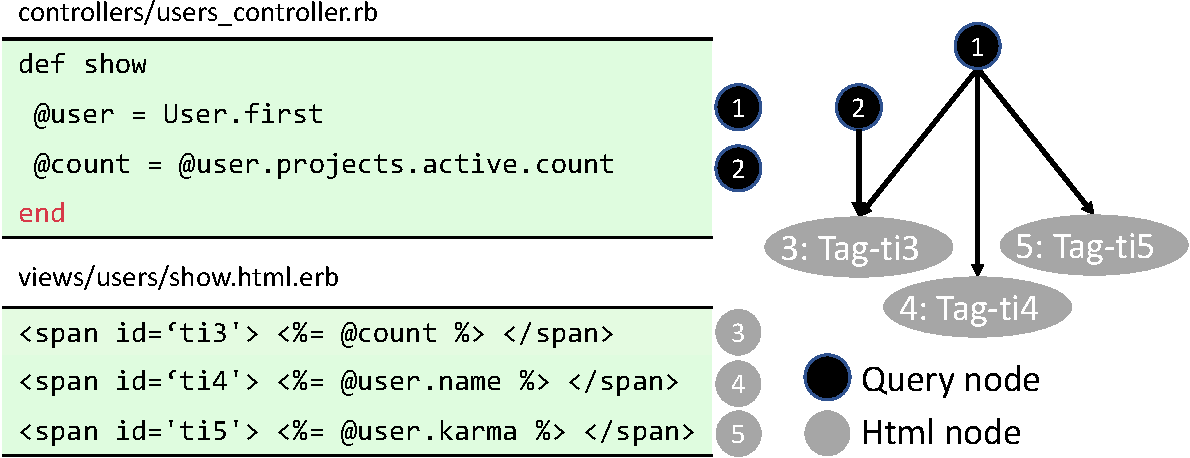
\includegraphics[width=0.7\columnwidth]{panorama-figs/code-example.pdf}
    \vspace{0.1in}
    \caption{Excerpt of an Action Dependency Graph}
    \label{fig:icq}
    \vspace{-0.2in}
\end{figure}

\subsection{Annotating the view component}
\label{sec:annotateview}
%\ToolP makes a few extension to the ADG generated by previous work 
%\cite{powerstation.fse18} for its view-centric analysis.
In order for \ToolP to attribute performance data correctly to each HTML tag,
\ToolP pre-processes every view file in the input web application
to assign every HTML tag a unique ID.
%through the HTML DOM (Document Object Mode). 
That is, for every tag {\tt <tag>} that does not already have an ID, 
\ToolP turns it into 
{\tt <tag id = ti>}, where {\tt ti} is a unique ID, as shown in the {\tt <span>} tags 
of Figure \ref{fig:icq}.
The current prototype of \ToolP does not handle HTML tags that are 
programmatically generated by JavaScript code.

%Next, while constructing the ADG, for every node coming from a view file, 
As mentioned, the view file has Ruby code embedded within it. For every node in ADG whose source code is in a view file,
\ToolP identifies its inner-most surrounding HTML tag and associates it with the corresponding tag ID.
\ToolP also %parses the view file to see 
checks whether its corresponding content is rendered or not by analyzing the HTML, and
assigns an {\tt is\_rendered} property accordingly. 
This information will help \ToolP attribute data processing cost to each HTML element and identify alternative view designs, as we will explain in later sections.
%\cong{Why is this necessary?}


%%%%%%% COMMENT OUT %%%%%%
\iffalse
The PDG generated above is then extended in three ways to create the ADG: 
(1) changing and splitting some nodes to become 
Query nodes; (2) annotating every Query node with the database table and fields that are read or written; 
(3) annotating every outgoing data-dependency edge of a Query node with the exact field(s) that are used.


To accomplish this, previous work first analyzes every model class that extends the Rails
{\tt ActiveRecord} interface to determine all the database
tables in the application and the association relationship among them.
For example, analyzing the model classes illustrated in 
Figure~\ref{fig:schema}, \ToolP identifies the {\tt users} table
corresponding to the {\tt User} class and similarly for the {\tt Blog} class, and that these two models have 
a one-to-many relationship, i.e., each instance of {\tt User} may own multiple instances of {\tt Blog}.
Second, \ToolP analyzes the {\tt schema.rb} file to determine
how many fields each table contains. For example, parsing the
{\tt schema.rb} snippet in Figure~\ref{fig:schema}, \ToolP learns about 
the schemas of table {\tt users} and {\tt blogs} as
shown in the bottom of the figure.

Third, \ToolP identifies queries from three sources: (1) explicit 
invocations of
Rails {\tt ActiveRecord} Query APIs, such as {\tt exist?},
{\tt reload}, \textit{\tt update}, \textit{\tt destroy}, etc;
(2) implicit queries generated by Rails to access object fields, e.g., {\tt $o_1$.$o_2$}, where 
the class of $o_1$ and the class of $o_2$ are associated model classes
(e.g., {\tt user.blogs} would incur a query to
retrieve records in {\tt blogs} table that are associated with
the specific {\tt user} record in {\tt users} table);
(3) explicitly invoked raw SQL queries through  Base.connection.execute.
%\junwen{it's also thru the ActiveRecord API, similar as the first type}
Any query identified above is represented as a Query node in the ADG.\footnote{At run time,
multiple such queries could be composed by ORM into one SQL query.
Such query chaining does not affect \ToolP analysis.}
\fi

\section{\Tool view-centric cost estimator} 
%\junwen{shall we change the title of this section? it seems profiling makes people confused about how we detect the optimization opportunities} \alvin{To me this is a bit confusing as profiling is used to describe both the overall process of finding contributing queries and estimating their costs, and also the `dynamic' profiling used given a test workload}
\label{sec:profile}

There are two key tasks in \Tool's cost estimation. First, given an HTML tag,
\Tool determines which database queries are executed
to generate the data that is rendered through that tag (we refer to them as contributing queries). 
Second, for each HTML tag, \Tool measures the data processing cost needed to render it.

While a web page's load time consists of client side rendering time,
network communication between client and server, 
computation time on the server, and database query cost,
\Tool's estimator currently focuses on database query cost, as query time often contributes a significant portion of the page load time. This is particularly true as the data size increases, and large query results lead to even more computation and rendering time. 
Query time/complexity is also
difficult for developers to estimate, particularly given the ORM abstraction.
As future work, we will incorporate other profiling tools to measure the performance of 
the client code \cite{chromeDev}, network, and server computation as part of \Tool.


\subsection{Identifying contributing queries}
\Tool identifies contributing queries for an HTML tag by statically analyzing
control and data dependencies in the ADG. Given an HTML tag in a view file, 
\Tool first identifies all ADG nodes $N$ that contain the tag's unique ID ---
these nodes contain the Ruby code embedded in the HTML tag. Then, \Tool 
 traces backward along the ADG edges to
identify all query nodes that any node in $N$ has control or data dependence upon. 
All these queries, each identified by its ADG node ID and Ruby source code
location, are considered as contributing queries of this HTML tag. 
For example, in Figure \ref{fig:icq}, tracing dependency edges backward from node 
{\large \textcircled{\small 3}}, which corresponds to HTML tag with id {\tt ti3}, %xx\shan{Junwen to fill}
will identify two contributing queries, nodes {\large \textcircled{\small 1}} and 
{\large \textcircled{\small 2}}.


\Tool further conducts forward dependency checking in the ADG to see how many other
HTML tags each query node contributes to. This number can be used
as a weight in computing the data processing cost of an HTML tag
--- if a query result is used to generate $k$ HTML tags
(e.g., the query node {\large \textcircled{\small 1}} contributes to three HTML tags in Figure \ref{fig:icq}), 
we could attribute $1/k$ of the query cost to each HTML tag if the web developers
choose so (while by default \Tool attributes the complete query cost to each tag).

\subsection{Cost analysis}

%\cong{Is it true that when dynamic profiling, you just replace the static query cost with the actual query running time? If so, I think it's better to introduce static estimation first (including the workflow of how you connect a query cost to a HTML tag), then dynamic.}\shan{Cong, I don't quite see why static
%analysis has to be placed first. The static analysis here is somewhat ad-hoc and more complicated to
%explain, so I feel it is better to discuss the clean dynamic profiling first.}

\Tool offers two modes of cost estimation with or without relying on testing workload.

\subsubsection{Dynamic profiling}
\label{sec:profile_dynamic}

If a testing workload is available, \Tool
will measure the cost of each contributing query during a 
testing run. However, using 
the query execution log from the backend database engine as the testing workload does not work ---
the database engine has no knowledge about frontend Ruby and HTML code, 
and hence does not allow \Tool to connect the statement in the web application that issues the query and the HTML tag uses the query result.

\Tool instead conducts its profiling through a hook API provided by Rails infrastructure, 
{\tt ActiveRecordQueryTrace}. This API allows its hooked code to be called before and after
issuing each SQL query. 
Using this mechanism, \Tool logs the amount of time of each query and the line of source code that
issues this query during the testing run, and attributes the time to the corresponding HTML tags using 
contributing query analysis as discussed above.


\subsubsection{Static estimation}
\label{sec:profile_static}
Since a bottleneck-exposing workload may not be available during in-house testing, \Tool also
uses static analysis to estimate the potential data-processing cost (in terms of its data complexity) to render each HTML tag.
For ease of estimation, \Tool assumes that all tables in the database have the same size $D$. 
%Future work can improve the estimation accuracy by refining this assumption.
Then, for each contributing query, \Tool estimates its complexity (i.e., how its execution
time might increase with $D$) by considering:
(1) the number of times this query might be issued, and
(2) time taken to execute one query instance.

To estimate the first factor, \Tool analyzes loops.
If the query $Q$ is not contained in any loop or is only contained by a loop whose 
iteration number does not increase with $D$, which we refer to as a {\it bounded loop}, 
\Tool then considers $Q$ to be executed for a constant number of times.
Otherwise, \Tool considers $Q$ to be executed for $D^k$ times, with $k$ being the number of {\it unbounded} loops containing $Q$.
To identify the {\it unbounded} loops, \Tool analyzes the bound variable 
of all loops that contain\ $Q$.
If the loop iterates through a set of records returned by an 
{\it unbounded} database query,
\Tool considers the loop to be unbounded.
Specifically, in Rails, a query is {\it unbounded} in all but the following
three cases:
(1) it always returns a single value, like a {\tt SUM} query; 
(2) it always returns a single record by selecting on primary key; %through the {\tt uniq} identifier; 
(3) it always returns a bounded number of records using the {\tt LIMIT} keyword.

To estimate the second factor, \Tool first identifies all the query operators
inside the query $Q$. For example, for the query node {\large \textcircled{\small 2}} in
Figure \ref{fig:icq}, \Tool would identify three query operators 
from the {\tt @user.issues.active.count} statement: 
a {\tt SELECT} to get {\tt issues}, 
another {\tt SELECT} to get {\tt active}, and finally a {\tt count} operator.
For most operators, we estimate its execution complexity to be $O(D)$.
There are a few exceptions:
we consider the complexity of a {\tt JOIN} operator to be $O(D^2)$, and 
the complexity of an operator that explicitly uses index, such as
{\tt find} and {\tt find\_by\_id}, to be constant. 
%\cong{{\tt find} does not explicitly use an index. we may say we assume tables have index on id and foreign key (or have index on every field), and every indexing operator has a constant cost.}

Putting these two factors together gives \Tool the complexity estimation
for one contributing query $Q$. For example, the estimated complexity of the 
query node {\large \textcircled{\small 2}} in Figure \ref{fig:icq} is O($D^3$). If it is
enclosed in an unbounded loop, its complexity would increase to O($D^4$).

\Tool could choose to deliver the above performance information using either a 
detailed text description or a numeric score. The current prototype
uses the latter: it uses the highest 
complexity among all contributing queries as the complexity score of an
HTML tag. For example, in Figure \ref{fig:icq}, 
the complexity score of HTML node {\large \textcircled{\small 3}} is 3, based
on the O($D^3$) complexity estimated for query node  {\large \textcircled{\small 2}}, and
the complexity scores of HTML node {\large \textcircled{\small 4}} and  {\large \textcircled{\small 5}}  are
both 1, based on the O($D$) complexity estimated for query node
{\large \textcircled{\small 1}}.

Of course, this is just a best-effort estimation from \Tool. There are 
several potential
sources of inaccuracy that can be improved by future work.
For example, some database tables may be much larger than others, which
we do not consider; the database can also lower the
query complexity than our estimation due to query optimization.

\iffalse
{\tt where}, 
{\tt all}, 
{\tt group}, 
{\tt join}, 
{\tt find}, 
{\tt includes}, 
{\tt teager\_load}, 
{\tt order}, 
{\tt count}, 
{\tt sum}, 
{\tt maximum}, 
{\tt minimum}, 
{\tt average}, 
{\tt having}, and 
{\tt calculate}. \cong{I think no need to mention query chain. Just say the SQL query type and how we estimate.}
\Tool currently assigns equal cost scores for each such operator.
\fi



 
%And the complexity will be decreased by 1 for limit, first,


\section{\ToolP view-aware optimization}
\label{sec:opt}
%\shan{Are we not doing incremental loading any more?}
%\cong{``\Tool optimization'' sounds a bit confusing (optimization to static analysis?). maybe ``Suggesting code change''?}\shan{I changed this and last section titles. How about now?}\cong{looks good! :)}


\Tool suggests three categories of view-changing code refactoring
to improve page-load time:

%\Tool categorizes view-changing performance optimization into three categories:
%, ranging from less to more changes to the view of a web application:
\begin{enumerate}
    \item Display the same contents in a different style, such as pagination and asynchronous loading.
    \item Display the same contents but with a different accuracy.
    \item Remove a subset of contents from display.
\end{enumerate}

These code refactorings can be applied for different types of HTML tags, and complement each other. 

\ToolP code refactoring works independently from \ToolP cost estimator. As we will see in Section \ref{sec:ide}, \ToolP interface will contain both features and help developers make informed refactoring decisions.\shan{How about this?}


% This section explains how \Tool automatically detects the opportunities
% and generates the code changes of the above three categories of optimization.
% Since these optimizations all improve performance with certain
% cost of functionality, \Tool will offer them in an interactive development environment as we will
% present in Section \ref{sec:ide}, instead of through transparent 
% code changes.

\subsection{Display-style change: pagination}
\label{sec:pagi}

Many web pages are designed to display {\it all} database records satisfying
certain conditions. When the database size grows, such pages will take an increasingly 
more time to load, and eventually become unresponsive.

A widely used solution to this problem, called {\it pagination}, is to display only a fixed number 
of records in a page and allow users to navigate to other pages for more records.

% \iffalse
% For example, Diaspora is a popular social network application \cite{diaspora}. 
% %Its {\tt contacts/index} page used to list {\it all} the contacts of a user, 
% One page from this application used to list {\it all} the contacts of a user,
% which led to slow page-loading time complained by users with many contacts. 
% Later on, in one issue report~\cite{diaspora5335}
% %Diaspora-5335~\cite{diaspora5335}, 
% developers solved this performance problem
% by showing contacts page by page, with 25 contacts a page. \shan{quantitative time information
% would help}
% \fi

Although pagination is widely used in practice, there are still many cases where it is not used --- 14 out of 140 real-world performance
issues sampled by a previous study \cite{yang:icse18:hloop} are due to lack of pagination
--- either because developers are unaware of pagination, or because they did not anticipate the data size will become a
performance problem. Therefore, we design \ToolP to automatically identify
pagination opportunities and conduct corresponding refactoring 
for developers. \alvin{isn't this what we do? last sentence makes it sound like this is future work}

\subsubsection{Identifying opportunities}


\begin{figure}
    \centering
    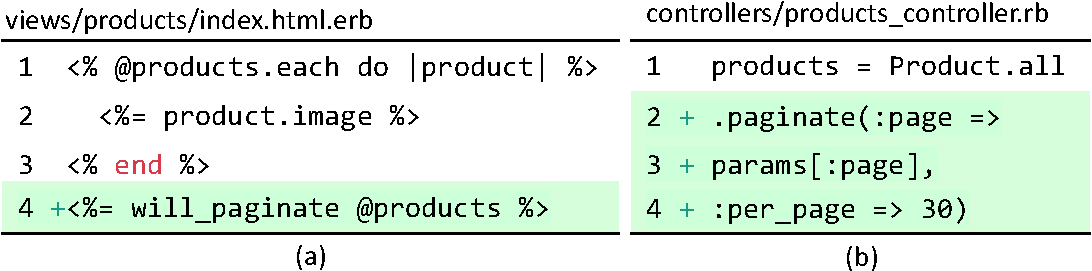
\includegraphics[width=\columnwidth]{panorama-figs//paginate.pdf}
    %\vspace{0.05in}
    \caption{Refactoring so that the paginated page displays 30 items at a time rather than the full list}
    \label{fig:pagi}
     \vspace{-0.2in}
\end{figure}

To identify these opportunities, \Tool checks each loop in the program for: (1) whether the loop iterates through the result of an unbounded query;
and (2) whether each loop iteration leads to some content being rendered in an HTML tag.
If a loop passes both checks, the corresponding HTML tag will be reported as a pagination candidate.

For the first check, \Tool locates the array variable that a loop iterates through, like {\tt @products} in
the loop shown in the left column of Figure \ref{fig:pagi}, and then
checks the data-flow edges in ADG to determine 
whether this variable is produced by an unbounded database query, as defined in Section \ref{sec:profile_static}.
For example, the ADG would show that {\tt @products} is the result of {\tt Product.all} on
Line~1 of in Figure~\ref{fig:pagi}b, and {\tt Product.all} will be translated to
an unbounded database query 
%which takes 1000ms \cong{what is 1000ms?}
at run time.

For the second check, \Tool searches for an ADG node $n_v$ that is associated with an HTML tag and an
{\tt is\_rendered} property inside the loop body (how to compute {\tt is\_rendered} is introduced in Sec. \ref{sec:annotateview}). If $n_v$ is found, like Line 2
in  Figure \ref{fig:pagi}a,
%(in both lines, the {\tt \%=} prefix 
%indicates that the Ruby variable following the prefix will be rendered),
the HTML tag associated with $n_v$ is identified as a pagination candidate.
%\cong{Can you give an example here?}

\subsubsection{Generating patches}
To carry out the refactoring,
\Tool performs two changes to the source code using the {\tt will\_paginate} library \cite{will_paginate}.
First, in the controller, \Tool adds a {\tt .paginate} call right after the
code statement where the to-be-rendered database records are retrieved, like
Line 2, 3 and 4 in  Figure \ref{fig:pagi}b. The constant there,
which is configurable and $30$ by default\alvin{how did you pick that?}, 
%\junwen{we use 30 here since it's the default value in the will\_paginate gem, developers can change the value according to themselves} 
determines how many records will be shown on every page.
Second, in view, \Tool adds a {\tt <=\% will\_paginate @products \%>} statement right
after the loop that renders these database records, as illustrated in Line 5 
 in Figure \ref{fig:pagi}a.
The {\tt will\_paginate} call inserts a page navigation bar into the web page, allowing users to navigate to remaining records after seeing the records displayed on the current page.

%Both changes can be easily automated by \Tool, as \Tool static analysis discussed
%above already identifies the record-retrieving query and the record-rendering
%loop.

%we check whether the {\tt Gemfile} has already included the {\tt will\_paginate} library, if not we will append it to the end of {\tt Gemfile}. {\tt Gemfile} is used to manage your application's Ruby dependencies. Secondly,





\subsection{Display-style change: asynch-loading}
\label{sec:async}

Asynchronous programming is widely used to support
low-latency interactive software \cite{okur2014study, okur2015study, lin2014retrofitting}. For web applications,
when there is an HTML tag that takes much longer time to render than other 
tags on the same page, we can instead compute and render the slow tag asynchronously, allowing users to see other parts of the web page more quickly.

For example, Discourse is a forum application. Its {\tt topics/show} page mainly
lists all the {\tt posts} that belong to a topic. At the bottom of that page after the listing of
all the {\tt posts}, a list of
{\tt suggested topics} that are related to this topic are displayed. 
In an issue~\cite{discourse4663}, users complained that this page is
slow to load no matter a topic contains many or few posts. 
Developers then realized that the query to retrieve suggested topics
is hurting the page-load time. Making things worse, these suggested topics
are not the main interests of this page and often are not seen by users, as they 
are placed below all the posts and require users to scroll down to the bottom of 
the page to see. %\cong{Don't get what ``do not come to users' view'' means.} 
Consequently, developers created a patch that defers the display of
{\tt suggested topics} until all other content on the page is
 displayed. 
%is deferred to display until the user reaches the end of the topic. As a result, even for shorter topics, it has the added benefit of reducing the first load time.


\subsubsection{Identifying opportunities}
\label{sec:async_op}
%\cong{change the title to ``Identify slow tags''?}
Conceptually, every HTML tag can be computed and rendered asynchronously. 
We only need to pay attention to two issues. 

First, only tags that are among the slowest on a web page are worthwhile for 
asynchronous loading. Otherwise, loading an originally fast tag asynchronously does not
help shorten the page load time, the \Tool estimator (Section \ref{sec:profile})
already provides information to help developers make this decision, and hence we do
not discuss this issue below.

Second, if too many HTML tags on a web page
are rendered asynchronously, the user experience could be greatly degraded. \alvin{why?}
Furthermore, if one HTML tag is rendered asynchronously, 
other HTML tags may better be rendered asynchronously too if they share a common 
contributing query. For example, in Figure \ref{fig:icq}, once we decide to load HTML tag
{\large \textcircled{\small 3}} asynchronously, {\large \textcircled{\small 4}} and {\large \textcircled{\small 5}} will be loaded asynchronously too,
as they share a common query {\large \textcircled{\small 2}}.
% \cong{It does seems to be a problem to me. If you detect slow tags by estimate the time, then tags share the same contributing query should be all slow and hence should be all detected.}
% \shan{Cong, the analysis here is NOT to detect slow tags. I added the previous paragraph that
% hopefully addresses this. Does it?}
% \cong{And how would multiple tags share a contributing query? If the query returns multiple records and rendered, then why this is not a problem for pagination? Otherwise if the query returns a number, why the tag is shown multiple times?}
% \shan{I added an example referring to Figure 4. I hope that answers your question.}
% \cong{Yes!}
\Tool considers this issue in identifying opportunities
for asynchronous loading, and we will describe how this is handled below.

\iffalse
for those tags which takes small amount time to load, doing so is not necessary. As a result, we identify those tags which take the top 3 performance cost in either wall-clock or relative measurement, and consider them as the one which can be loaded asynchronous or removed.
\fi

\subsubsection{Generating patches}
Given an HTML tag $e$, making its content computed and rendered
asynchronously requires multiple changes
to the controller and view components of a web application,
as illustrated in Figure \ref{fig:async}:
(1) creating a new view file that renders $e$ only, separating $e$
from other tags on the same web page that will still be synchronously loaded;
(2) adding a new controller action to compute {\it all and only} the content 
needed by $e$ and render the new view file created above, separated from the computation
for other tags on the same web page that will still be carried out synchronously; 
(3) replacing $e$ in the original view file with an AJAX request and 
adding a new routing rule so that the AJAX request will invoke the
new action in (2) which then renders the view in (1) asynchronously.
% \cong{Can you describe it in a more general way? People may not understand why do you need a new partial-view file or new action, that's too much detail for those who do not know Rails. }
% \shan{how about now?}
% \cong{looks good!}

\begin{figure}
    \centering
    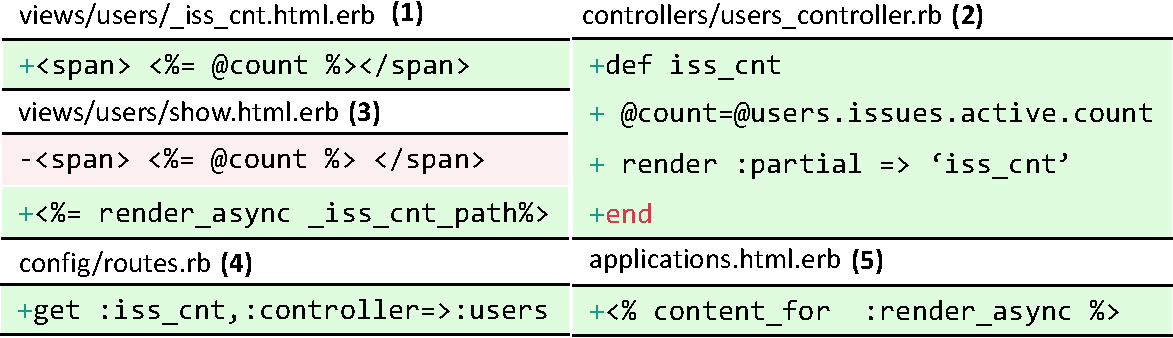
\includegraphics[width=\columnwidth]{panorama-figs/async.pdf}
    \caption{Refactoring for asynchronous loading}
    \label{fig:async}
     \vspace{-0.2in}
\end{figure}

The first item is straight-forward to automate.
\Tool simply moves the HTML tag $e$ into a newly created view file,
like {\tt \_iss\_cnt.html.erb} (Figure \ref{fig:async}(1)), where {\tt iss\_cnt} corresponds to the 
name of the new controller action that \Tool will generate. 



The second item 
%is non-trivial
%and could be error-prone for developers
%to carry out manually. 
is implemented by \Tool in three steps.
It first identifies all Ruby variables
used by $e$, like {\tt @count} in Figure \ref{fig:async}(1), and then
applies static backward slicing to find all code statements $C$
that are used to compute those variables, like
{\tt @count = @user.issues.active.count} in Figure \ref{fig:async}.
Specifically, \Tool starts from all the ADG nodes associated with
the specific HTML-tag ID, and traces backwards in the ADG to identify all nodes inside the corresponding
controller that $e$ has control or data dependence on.

\Tool next applies forward taint analysis to see if any statement $c \in C$
is used to compute any other HTML tag $e'$. If such an $e'$ is
found, there is a dilemma about whether to render $e'$ asynchronously: 
rendering $e'$ asynchronously could potentially
cause many other HTML tags, which share common backward slicing
fragments with $e'$, to be rendered asynchronously, and violate the 
design principle discussed in Section \ref{sec:async_op}; yet rendering $e'$ synchronously
incurs extra overhead as $c$ now needs to be computed twice,
%could cause server-resource wasting\cong{``server resource'' sounds strange, as resource usually means memory/bandwidth/..., and I think here it means server time?}, as $c$ now needs to be computed twice,
once for $e$ and once for $e'$. 
Hence, \Tool currently considers $e$ as unsuitable for asynchronous loading if $e'$ exists. 
%Of course, future extension of \Tool can be more flexible
%and introduce a threshold,
%like making no more than $K$ elements asynchronous at a time.

\Tool finally moves the slice identified earlier to a new controller action, like
{\tt iss\_cnt} in Figure \ref{fig:async}(2) (the deletion from the previous controller is not shown for simplicity), and add a rendering statement
at the end of the action,
like  {\tt render :partial => `iss\_cnt'} in Figure \ref{fig:async}(2),
to render the same content
in the same format as the original web application using the newly created view file.

\Tool conducts the third item leveraging the {\tt render\_sync} library \cite{asyncgem} to replace the original HTML tag with 
``{\tt<\%= render\_async [action]}
{\tt \_path \%>}'' (Figure \ref{fig:async}(3)), where {\tt render\_async}
is an API call that issues an AJAX request for the specified
{\tt action} using jQuery~\cite{jquery}.
\Tool then adds a new rule into the routing file
to connect the AJAX request with the action it just created.
As shown in  
Figure \ref{fig:async}(4), this new routing rule follows the template
``{\tt get :[action], :controller =$>$} {\tt :[home]}'', 
where {\tt action} is the name of new action name, and 
{\tt home} is the controller holding the {\tt action}.


\subsection{Display-accuracy change: approximation}
\label{sec:approx}

\begin{figure}
    \centering
    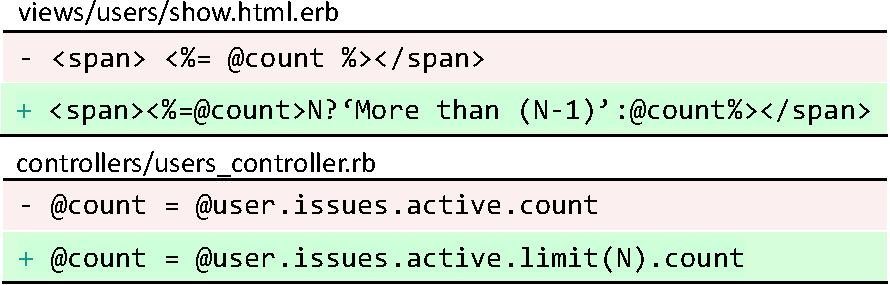
\includegraphics[width=\columnwidth]{panorama-figs/approxi.pdf}
    \caption{Refactoring for approximation}
    \label{fig:approxi}
    \vspace{-0.2in}
\end{figure}

Approximation is a widely used approach to improving performance and saving server resources \cite{farrell2016meantime}. 
Past database research also proposed approximated
queries \cite{motwani:cidr03:query}. However, many techniques require 
changes to database engines \cite{ioannidis:vldb99:histogram} and hence
cannot be applied to web application refactoring. \Tool focuses on approximating
aggregation queries whose results are displayed as numeric values on web pages,
as such approximation can be simply conducted by refactoring Rails code
and easily reasoned about by web viewers.

For example, 
Redmine \cite{redmine} is a project collaboration application like GitHub. Its  {\tt user/index} page
lists all the recent activities of a user, all projects a user is involved in (with pagination), 
as well as two 
counts showing how many issues are currently assigned to and have been reported by 
this user.
%, as shown in Figure~\ref{fig:redmine}. 
Although these two numerical counts occupy tiny space on the web page,
they can take more time, even more than 1 second, to render than the remaining page,
when a user is involved in hundreds of or more issues. 
One way to keep the page responsive is to set an upper-bound to such a count, like $100$, and only
shows the count to be ``{\it more than 100}'' when it is too big --- when a count is too big,
 users probably does not care about the exact number anyway.

\iffalse
\begin{figure}
    \centering
    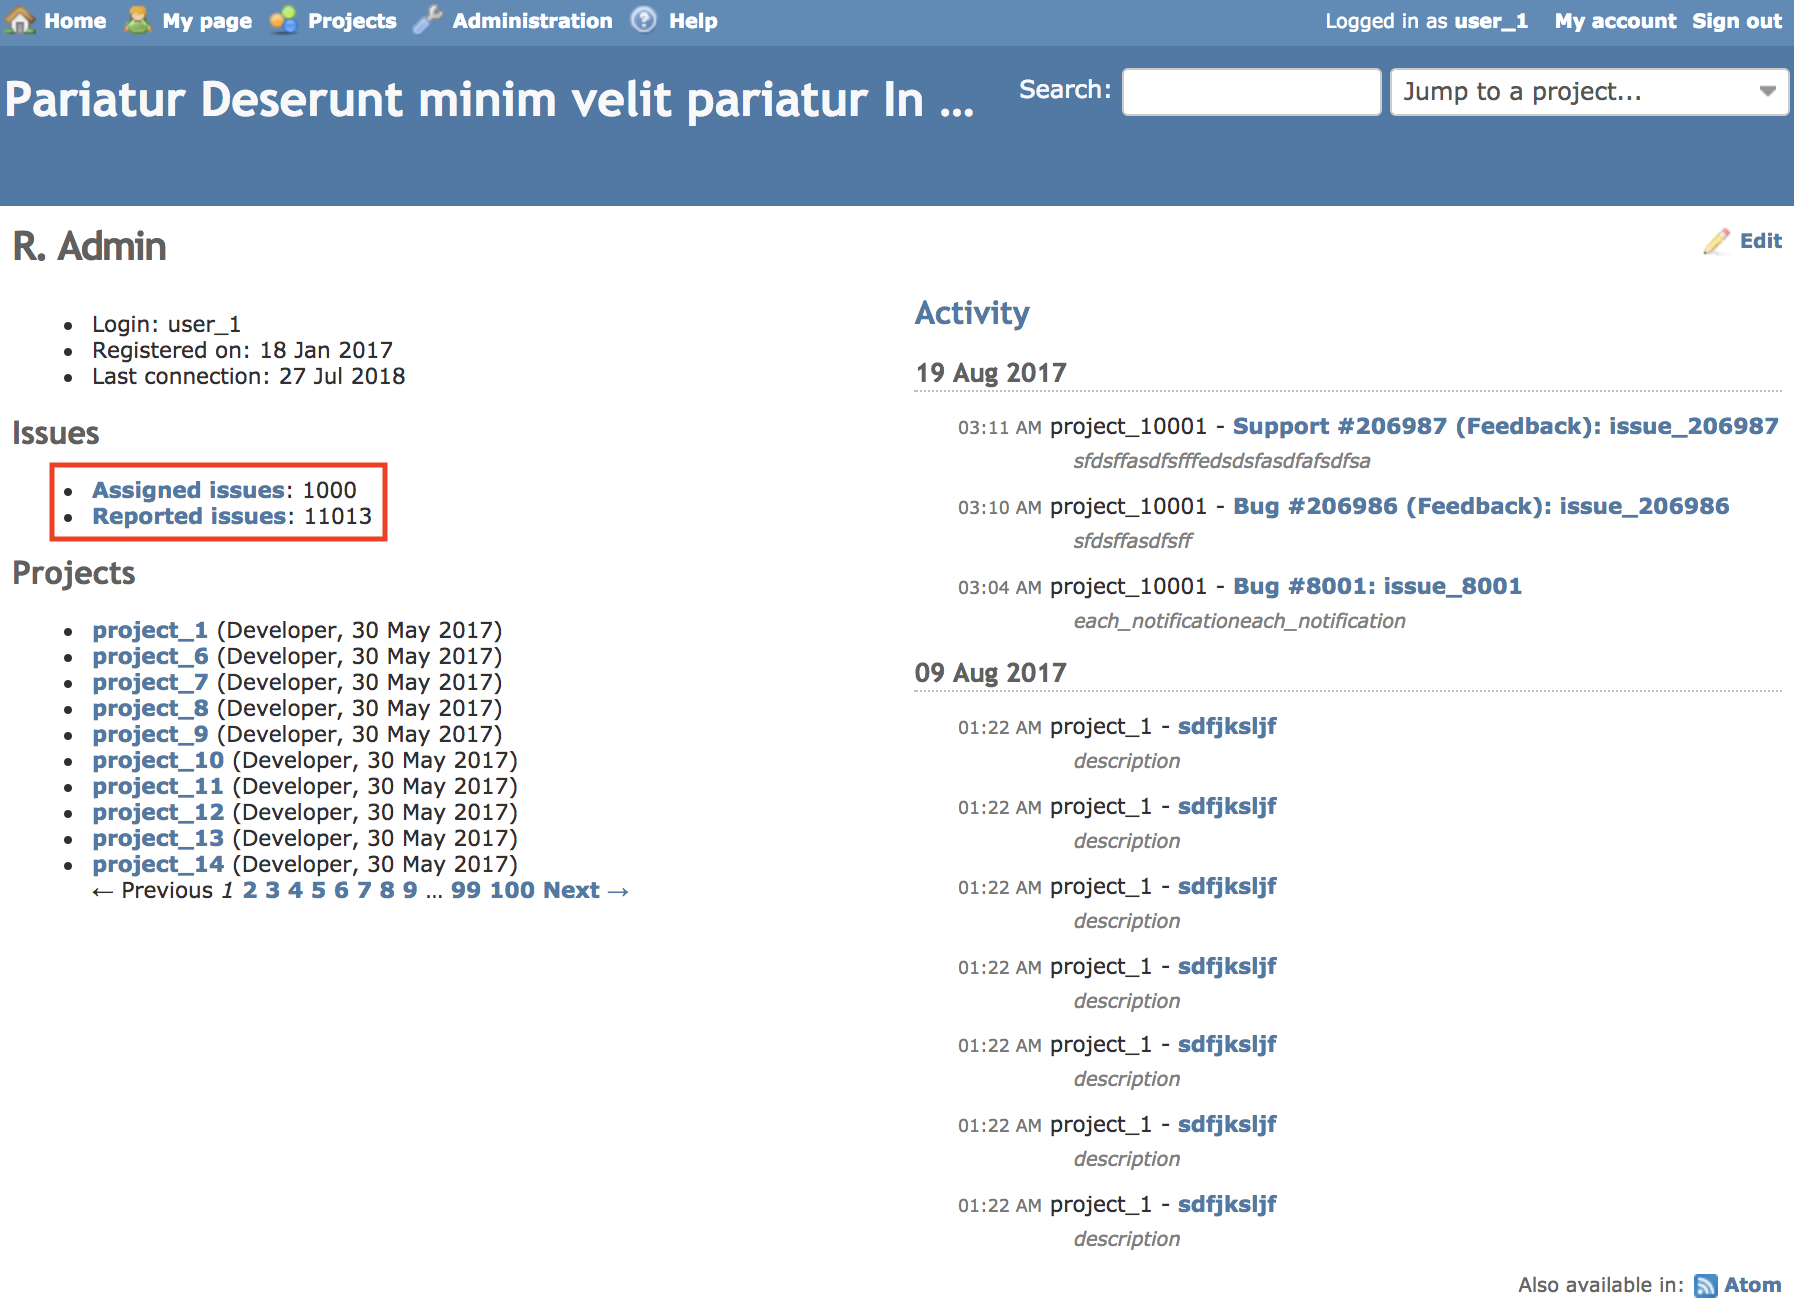
\includegraphics[width=\columnwidth]{figs/redmine.png}
    \caption{Redmine users/1 page}
    \label{fig:redmine}
\end{figure}
\fi

\subsubsection{Identifying opportunities}
\Tool iterates through all aggregation, including
maximum, minimum, average, and count,
queries in the application. 
For each query, \Tool checks its corresponding ADG node's
out-going data-flow edges to
see if the query result is {\it only} used in
HTML-tag rendering. 
If so, an approximation opportunity is
identified for corresponding HTML tag(s). 
Note that, \Tool does not suggest approximating an aggregation query if its result affects
an HTML tag through control dependency, as that type of approximation may
cause program execution to take a different path and hence potentially leads
to large deviation from original program behaviors. 
%\cong{why?}\shan{err, I revised a little bit.
%is it clear now?}\cong{yes}

\subsubsection{Generating patches}
An approximation refactoring includes two parts. 
On the controller side, \Tool appends a {\tt limit(N)} clause to the end of the
aggregation query identified above, with the constant $N$ configured by 
web developers. On the view side, instead of directly displaying the
numeric query result, changes are made depending on the aggregation query type.
For a {\tt count} query, \Tool inserts a conditional statement to check the aggregation result: if the result is smaller than $N$ then the accurate numerical result is displayed, otherwise
``more than $N-1$'', as shown in Figure \ref{fig:approxi};
for an average query, \Tool adds ``{\tt about}'' before the numeric query
result rendered in the HTML tag; for a maximum or minimum query,
\Tool adds ``{\tt at least}'' or ``{\tt at most}'' before the numeric query
result.



\subsection{Display contents removal}

Obviously, one can remove an HTML tag to speed up the page loading. 
This strategy is indeed used in practice, as the {\tt Tracks} example discussed in
Section \ref{sec:intro}.
Whether an HTML tag is worthwhile to display cannot be determined automatically.
Instead, what \Tool can do is to make the removal easy and error-free, so that developers
can easily try out different design options and eventually make an informed decision.

% \iffalse
% For example, a popular task-management application Tracks \cite{tracks} has a
% %{\tt todos/index} page. The {\tt todos/index} page mainly 
% page that lists the todos in the left pane. This page %and it 
% has a right sidebar to retrieve and display all the projects and contexts of the
% current user, which takes a lot of time for user who takes part in large number of projects. In the side-bar code, the only data-related \cong{data-related?} part
% is simply a {\tt @sidebar.active\_projects} and a {\tt @sidebar.active\_contexts} statement, which seem
% like \cong{why mention ``seem like...'' and why mention these two statements (I assume they are function calls but you do not explain what's in the function)?} a trivial heap access but actually issue a {\tt SELECT} query and
% retrieves the projects and contexts. Later on in tracks-870, the developers made a trade-off between performance
% and functionality by deleting the sidebar completely,
% %and not showing users the projects and contexts. 
% \shan{how many? how can a user be involved in many projects? What is the expensive query behind} \junwen{The complain says he has 80 projects which will grow pu to 150 projects later on}
% %to render. Eventually, developers decided to delete this side-bar completely, %which 
% providing xxx speed-up to this web page. 
% \fi
 
\subsubsection{Identifying opportunities}
Removing an HTML tag $e$ does not guarantee to save page-loading time, because if the expensive
computation needed by $e$ is also needed by other HTML tags, removing $e$ alone will not help
performance much. The current prototype of \Tool only suggests removing an HTML tag $e$ if its contributing query that is not fed to any other HTML tag.
%\cong{if so, how do you remove a sidebar that contains many elements?}
%\shan{currently, we just don't unless those items are displayed inside one HTML tag}. 
This way, removing $e$ can guarantee to save some data-processing time.
Of course, future work can relax this checking criterion.
\begin{figure}
    \centering
    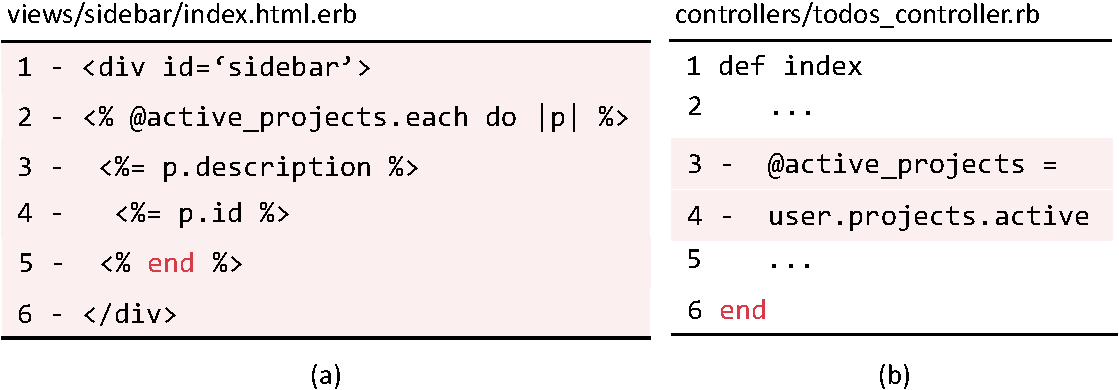
\includegraphics[width=1\columnwidth]{panorama-figs/remove.pdf}

    \caption{code change for removing}
    \label{fig:remove}
    \vspace{-0.2in}
\end{figure}

\subsubsection{Generating patches}
Removing an HTML tag $e$ from the web page again involves changes to both the
view component and the controller component of a web application.
On the view side, \Tool simply removes the specific HTML tag.
On the controller side, \Tool again analyzes control-dependency and data-dependency graph
to remove code that was used only to help generate $e$.

To do so, \Tool first identifies all the nodes in ADG that are associated with $e$'s ID.
\Tool deletes those nodes, removes all condition checking whose two branches
now execute exactly the same code because of those node deletions, and then 
check if there are any other ADG nodes that
become useless and should be deleted
--- a node is useless if it has no out-going data-dependency or control-dependency
edges. \Tool repeats
this process for several rounds until no more nodes are identified as useless. 

We use the view file code snippet in Figure \ref{fig:remove}a as an example.
The HTML tag shown here corresponds to the sidebar
that lists all projects 
in the Tracks example discussed in 
Figure \ref{fig:crossstack}.
%, as shown in Figure\ref{fig:heatmap}
Given this tag, \Tool first identifies the
Ruby expression {\tt @active\_projects}, and then checks the ADG to see how 
{\tt @active\_projects} is computed in the
controller (Figure \ref{fig:remove}b).
\Tool also finds out that the 
{\tt @active\_projects} computed in 
Figure \ref{fig:remove}b is not used in anywhere
else.
%\shan{What is
%show-guidelines? Is this a function or what?}, and
Consequently, the content-removal change will simply
delete the sidebar tag in the view file
%computing statement
and the corresponding computation
in the controller file, as shown in 
Figure \ref{fig:remove}.


%\shan{can we extend this to removing the condition checking of a HTML element display?}

%\iffalse

%\fi

\section{The \Tool Interface}
\label{sec:ide}
\label{sec:im}
\begin{figure}
    \centering
   
    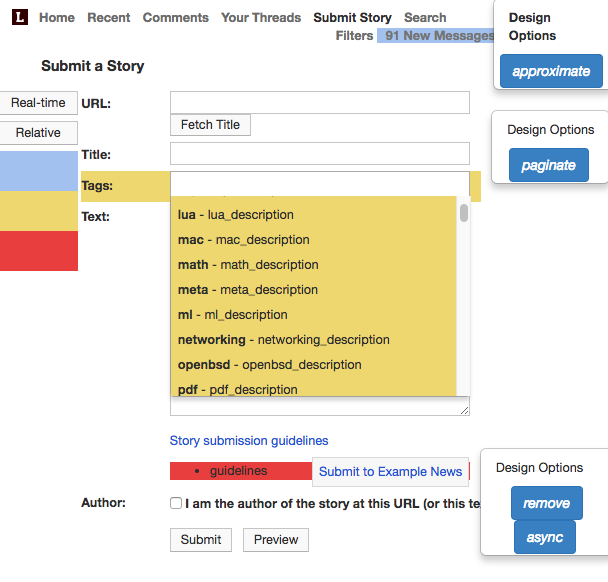
\includegraphics[width=\columnwidth]{panorama-figs/heatmap.png}
    \vspace{-0.1in}
    \caption{An example of \Tool browser interface}
    \label{fig:heatmap}
     \vspace{-0.2in}
\end{figure}

%Given the view-centric profiling (Section \ref{sec:profile}) and view-aware optimization  (Section \ref{sec:opt}) are available, 

\Tool comes with a new interface to present the cost estimation and optimization information, and help developers explore different web-page design options. We discuss the \Tool interface in this section.

%We have implemented our approach into a RubyMine  plugin.


\subsection{Information display in browser}
\label{sec:ide_browser}
\textbf{Showing view-centric cost estimation information.}
\Tool visualizes the performance information obtained by dynamic profiling or 
static estimation (Section \ref{sec:profile}) through a heat-map with the more costly
HTML element having a more red-ish background, as illustrated in
Figure \ref{fig:heatmap}.

To generate this heat map, \Tool reads the output of its 
view-centric cost estimation (Section \ref{sec:profile}) 
and creates a JavaScript file {\tt interactive.js} that 
sets the background color
of every HTML tag through
``{\tt \$(tag-id).css(``background-color'', color);}'', where {\tt tag-id} is the
unique HTML tag ID and {\tt color} is computed based on the cost estimation for this HTML tag (Section \ref{sec:profile}).
Web developers can choose to see different heat-maps with
buttons on the web page, like ``Real-time'' (dynamic profiling
results) and ``Relative'' (statically estimated results) 
in Figure \ref{fig:heatmap}. We set the color using the HSL color scheme, with
more expensive tags rendered with smaller hue values (i.e., more red-ish) and
cheaper tags with larger hue values (i.e., more blue-ish).
\iffalse
Hue represents the degree on the color wheel ranging from 0 to 360, 0 is red, 120 is green, and 240 is blue. We order the tags through their performance cost in the ascendant order, and get the total number of costs as N, then we calculate the color gradient as {\tt scale = 1.0 / (N - 1)}, and the color for tags in rank index will be 240 * (1 - i * scale). As a result, the larger the performance cost is, the HUE will be closer to 0 which means that it is be more red-ish, and the smaller the performance cost is, HUE will closer to 240 as known as more blue-ish.   
\fi


\iffalse 
\begin{figure}[h]
    \centering
    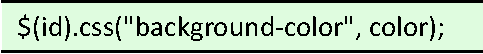
\includegraphics[width=\columnwidth]{figs/background.pdf}
    \caption{setting background color using javascript}
    \label{fig:bgchange}
\end{figure}
 \fi
 


\textbf{Showing view-aware optimization suggestions.}
%The JavaScript file created by \Tool above 
{\tt interactive.js} described above
helps display not only 
data-processing cost but
also alternative view-design options for various HTML tags. 
Users simply right click
an HTML tag in the browser to get a list of design options, as shown in Figure \ref{fig:heatmap}.
The implementation is straight-forward,
given the unique ID of every HTML tag and the performance-enhancing opportunities
identified through \Tool static analysis as discussed in Section \ref{sec:opt}.

\begin{figure}
    \centering
    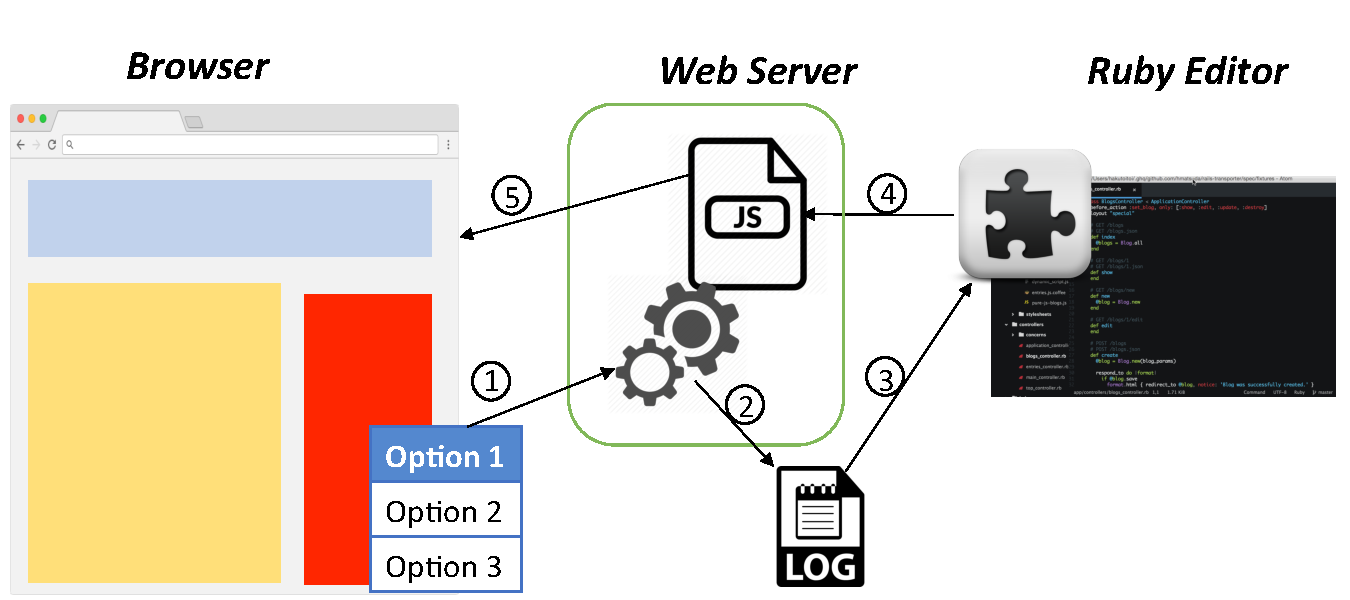
\includegraphics[width=\columnwidth]{panorama-figs/interface.pdf}
    \caption{\Tool interface implementation}
    \label{fig:interaction}
     \vspace{-0.2in}
\end{figure}

\subsection{Design-space exploration in browser}
To help developers explore different
performance--functionality design trade-offs, \Tool further
connects the browser-side information display and the Ruby editor side
refactoring together:
(1) developers first understand the data-processing cost 
of various HTML tags in the browser; 
(2) once developers choose an alternative design option for an HTML tag, 
the corresponding code refactoring will be automatically applied and displayed 
in the accompanying Ruby editor for developers to review; 
(3) once the source code is updated, the heat-map in the browser is
updated accordingly. Developers can explore different
design options, and eventually pick the best ones that suit their need.

To support this interface, \Tool carefully uses JavaScript, IDE plugin, and
other mechanisms
to help the communication between the browser and the Ruby editor, as illustrated
in Figure \ref{fig:interaction}.\footnote{The current prototype of \Tool assumes that the web-application under testing is deployed
on the same machine as the Ruby editor.}

First, \Tool automatically instruments the web application under development to help
communicate developers' design choices to the Ruby editor. Specifically, \Tool
adds a controller {\tt \_PANO\_handle\_request}
into the web application. Whenever developers click a design-option button,
like one of those blue {\it paginate}, {\it async}, {\it approximate},
{\it remove} buttons in Figure \ref{fig:heatmap}, 
\Tool
%the \Tool JavaScript file
%(i.e., the same one that creates the heat-map)
will send an HTTP request to invoke the {\tt \_PANO\_handle\_request} 
controller action ({\large \textcircled{\small 1}}  in Figure \ref{fig:interaction}), 
which then records the design-option type and the corresponding
HTML tag ID into a web-server side file {\tt request.log} ({\large \textcircled{\small 2}} in Figure \ref{fig:interaction}). 

In the editor, which we use RubyMine \cite{rubymine}, \Tool 
%creates an IDE plugin that 
uses a thread to monitor the {\tt request.log} file.
Whenever this file is changed, this monitoring thread will trigger the 
plugin to apply corresponding code refactoring in the IDE, with all the
code changes generated using algorithms described in Section \ref{sec:opt}
({\large \textcircled{\small 3}}  in Figure \ref{fig:interaction}). 

After the code change, the data-processing cost estimation will be updated automatically, which results in updates to a performance profile 
%{\tt log/development.log}
and corresponding updates to {\tt interactive.js} %\Tool JavaScript file
with changed background-color settings ({\large \textcircled{\small 4}}  
in Figure \ref{fig:interaction}).
%The changes in the JavaScript file will lead to 
The changes in {\tt interactive.js} lead to
an automated refresh in the browser with the updated heat-map display, as we use  the Ruby 
{\tt react-rails-hot-loader} to enable
automated refresh at every change in the Ruby source code or 
heat-map display code
%the \Tool JavaScript code 
({\large \textcircled{\small 5}}  in Figure \ref{fig:interaction}).



% Our current implementation using RubyMine \cite{rubymine}, one of the most popular Ruby on Rails
% IDE. \Tool's RubyMine plug-in uses
% IntelliJ APIs, like {\tt FileEditorManager}, {\tt TextRange}, and {\tt Document},
% to insert, replace, and delete source code in the code editor panel of RubyMine.  



\section{Evaluation}

\label{sec:eva}
Our evaluation focuses on four research questions:
{\bf RQ1}: Can \Tool identify view-aware optimization opportunities from latest versions
    of popular web applications?
{\bf RQ2}: How much performance benefits can view-aware optimization provide?
{\bf RQ3}: Is the performance-functionality trade-off space exposed by \Tool worthwhile for developers to explore?
{\bf RQ4}: Does \Tool estimator estimate the per-tag data-processing cost accurately?
\begin{table}[t]											
\centering											
\caption{Opportunities detected by \Tool in 12 apps}												
\label{tab:oppo}										\centering
\resizebox{0.6\columnwidth}{!}{%
\begin{tabular}{@{}lrrrrrrrrrrrrr@{}}
\toprule
App	&	Ds	&	Lo	&	Gi	&	Re	&	Sp	&	Ro	&	Fu	&	Tr	&	Da	&	On	&	FF	&	OS	&	SUM	\\	\midrule
pagi.	&	1	&	6	&	1	&	10	&	2	&	20	&	5	&	9	&	1	&	6	&	3	&	3	&	69	\\	\midrule
approx.	&	1	&	1	&	0	&	7	&	0	&	5	&	1	&	3	&	0	&	23	&	0	&	0	&	43	\\	\midrule
removal	&	1	&	2	&	0	&	7	&	0	&	4	&	1	&	2	&	2	&	2	&	0	&	0	&	22	\\	\midrule
asynch	&	1	&	2	&	0	&	2	&	0	&	2	&	1	&	2	&	2	&	2	&	0	&	0	&	15	\\	\midrule
SUM	&	4	&	11	&	1	&	26	&	2	&	31	&	8	&	16	&	5	&	33	&	3	&	3	&	149	\\	
 \bottomrule
\end{tabular}

}	
\end{table}

\begin{table}[h]
\centering
\caption{Speed up of 15 view changes}
\label{tab:speedup}
\resizebox{\columnwidth}{!}{%
\begin{tabular}{@{}l|rrrrrr|rr|rrrr|rrr@{}}
\toprule
%  & \multicolumn{6}{|c|}{Pagination} & \multicolumn{4}{c|}{Approximation} & \multicolumn{3}{c|}{Content Removal} & \multicolumn{2}{c}{ Asynchronous} \\ \midrule
% ID & Ro1 & Tr1 & Fu1 & Re2 & On1 & Re1 & Re2 & On2 & Tr2 & On3 & Lo1 & Re3 & On4 & Lo2 & On5 \\ \midrule
% Server Time Speedup (X) & 19.4 & 13.5 & 6.8 & 4.7 & 2.1 & 1.8 & 2.1 & 1.4 & 1.2 & 1.3 & 33.0 & 1.4 & 1.1 & 37.8 & 1.1 \\ \midrule
% End-to-End Time Speedup (X) & 9.4 & 9.2 & 5.9 & 3.6 & 2.7 & 1.6 & 1.6 & 1.3 & 1.2 & 1.0 & 8.7 & 1.3 & 1.2 & 17.2 & 1.2 \\
&	\multicolumn{6}{|c|}{Pagination}	&	\multicolumn{2}{c|}{	Asynchronous}	&	\multicolumn{4}{c|}{Approximation}	&	\multicolumn{3}{c}{Content	Removal}	\\	\midrule																													
ID	&	Ro1	&	Tr1	&	Fu1	&	Re2	&	On1	&	Re1	&	Lo2	&	On5	&	Re2	&	On2	&	Tr2	&	On3	&	Lo1	&	Re3	&	On4					\\	\midrule				
Server Time Speedup (X)	&	19.4	&	13.5	&	6.8	&	4.7	&	2.1	&	1.8	&	37.8	&	1.1	&	2.1	&	1.4	&	1.2	&	1.3	&	33	&	1.4	&	1.1					\\	\midrule				
End-to-end Time Speedup (X)	&	9.4	&	9.2	&	5.9	&	3.6	&	2.7	&	1.6	&	17.2	&	1.2	&	1.6	&	1.3	&	1.2	&	1	&	8.7	&	1.3	&	1.2					\\					
\bottomrule
\end{tabular}
}
{Every case is denoted by $<$application-short-name$>$-ID}
\end{table}

\begin{table*}[th]
\centering
\caption{Database sizes and page load time of 12 user-study cases}
\label{tab:dbsize}	
\resizebox{1\columnwidth}{!}{%
%\begin{tabular}{@{}l|ggg|ggg|ggg|ggg@{}}
\begin{tabular}{@{}l|ccc|ccc|ccc|ccc@{}}
\toprule
 & \multicolumn{3}{c|}{Pagination} & \multicolumn{3}{c|}{Asynchronous}  & \multicolumn{3}{c|}{Approximation}  & \multicolumn{3}{c}{Content Removal} \\ \midrule
\rowcolor{white}
ID & Re1 & {\color[HTML]{FE0000} Ro1} & Tr4 & Re4 & {\color[HTML]{FE0000} Tr3} & Lo1  & Re2 & Tr1 & Di1 &  Lo2 & {\color[HTML]{FE0000} Tr5} & Tr6
\\
\midrule
\rowcolor{white}
DB Size (k-record) & 2 & 0.8 & 2 & 2 & 2 & 20 &  100 & 100 & 100 &  20 & 100 & 2 \\ \midrule
\rowcolor{white}
Base Page Load Time (s) & 2 & 1.9 & 2.5 & 2 & 1.9 & 1.8  & 2.5 & 2.5 & 2.5 &  1.8 & 2.5 & 1.9 \\ 
\rowcolor{white}
New Page Load Time (s)  & 0.5 & 0.4 & 1  & 0.5 & 0.4 & 0.3 &  1 & 1 & 1  &  0.3 & 1 & 0.4 \\
\midrule


\end{tabular}
}

\footnotesize{3 red IDs are cases from existing issue-tracking systems; the other 9 cases are all in latest versions discovered by \Tool.\\ Every case is denoted in the same way as Table \ref{tab:speedup}, with 6 common cases.} 
 \vspace{-0.2in}
\end{table*}
\subsection{Methodology}
{\bf Applications.}
We evaluate \Tool using a suite of 12 open-source Ruby on Rails applications as shown in Table~\ref{tab:apps}.

{\bf Workload.} Since we cannot obtain real-world user data, we use synthetic data generation
scripts released by previous work that to populate the databases following real-world
data distribution and statistics.
%Following previous work~\cite{yang:icse18:hloop}, 
Similar to~\cite{yang:icse18:hloop},
we use the number of records in a web application's
main database table to describe the workload size. By default, we use a 20,000-record workload
unless otherwise specified.
To our best knowledge, {\bf all} the database sizes used in our evaluation
are similar or smaller than the sizes in real-world web applications.%\cong{Is it OK that we cite the hyperloop paper so frequently? Will anyone complain it will disclose our identity?}

{\bf Platform.} We profile the Rails applications on AWS Cloud9 platform~\cite{awsc9}, which has 2.5GB RAM and a 8-core CPU. 




% big version for table1
\iffalse
\begin{table}[]
\centering											
\caption{Opportunities detected by \Tool in 12 apps}												
\label{tab:oppo}		
\begin{tabular}{@{}lrrrrr@{}}
\toprule
App & \multicolumn{1}{l}{pagination} & \multicolumn{1}{l}{approximation} & \multicolumn{1}{l}{asynch} & \multicolumn{1}{l}{removal} & \multicolumn{1}{l}{SUM} \\ \midrule
Ds & 2 & 3 & 1 & 1 & 7 \\ \midrule
Lo & 4 & 0 & 1 & 0 & 5 \\ \midrule
Gi & 1 & 0 & 0 & 0 & 1 \\ \midrule
Re & 9 & 3 & 7 & 6 & 25 \\ \midrule
Sp & 2 & 0 & 0 & 0 & 2 \\ \midrule
Ro & 14 & 4 & 4 & 4 & 26 \\ \midrule
Fu & 7 & 1 & 1 & 1 & 10 \\ \midrule
Tr & 10 & 3 & 2 & 2 & 17 \\ \midrule
Da & 1 & 0 & 2 & 2 & 5 \\ \midrule
On & 6 & 25 & 2 & 2 & 35 \\ \midrule
FF & 6 & 2 & 4 & 1 & 13 \\ \midrule
OS & 3 & 0 & 0 & 0 & 3 \\ \midrule
SUM & 65 & 41 & 24 & 19 & 149 \\ \bottomrule
\end{tabular}
\end{table}
\fi

\subsection{RQ1: how many opportunities does \Tool identify?}
\label{sec:rq1}
As shown in Table \ref{tab:oppo}, \Tool can indeed identify many view-aware
optimization opportunities.
Specifically, \Tool static analysis identifies \alvin{what does statically identify mean?} \junwen{Panorama detects all optimization opportunities through static analysis and does not rely on any dynamic profiling. We may add more explanation in section V} \numissues performance-enhancing
opportunities from the current versions of our benchmark applications. 
Every type of optimization 
opportunities is identified from at least 8 applications.

These 149 opportunities apply to 119 unique HTML tags. 
For 101 HTML tags, only one view-change suggestion is made.
For the remaining 18, \Tool suggests two or three changes.
Particularly, there are 15 HTML tags where {\it removal} and {\it asynchronous}
loading both apply. 
%Although pagination is the most commonly suggested one, the other three types
%are also common. \cong{This sentence seems redundant.}
Overall,
these four types well complement each other.

\subsection {RQ2: how much performance benefits?}
\label{sec:rq2}

To quantitatively measure the performance benefits of these alternative
view designs,
we randomly sampled 15 optimization opportunities identified above, 
with 6, 2, 4, and 3 cases from Pagination, Asynchronous (loading), Approximation, and Content Removal 
respectively,\alvin{why are only some of the words italized?}\junwen{this is to be matched with the table II and table III} \alvin{then it should be `pagination [\bf{pagination}]' etc} in 6 different applications. \junwen{How we do the speed up measurement:} For each application, before and after optimization, we run a Chrome-based crawler that visits links randomly for 2 hours and measure the average end-to-end-latency and server-cost of every action. We then compute speedup accordingly.
\iffalse
\begin{table}
\centering
\caption{Speed up of 15 view changes (S: server side speed-up; E: end-to-end page-load time speedup)\shan{font too small.}}
\label{tab:speedup}
\resizebox{\columnwidth}{!}{%
\begin{tabular}{@{}l|r|l|l|l|l|l|r|l|l|l|r|l|l|rl@{}}
\toprule
 & \multicolumn{6}{c|}{pagination} & \multicolumn{4}{c|}{approximation} & \multicolumn{3}{c|}{asynch} & \multicolumn{2}{c}{removal} \\ \midrule
S & \multicolumn{6}{r|}{19x 14x 6.8x 4.7x 2.1x 1.8x} & \multicolumn{4}{r|}{2.1x 1.4x 1.2x 1.3x} & \multicolumn{3}{r|}{33x 1.4x 1.1x} & \multicolumn{2}{r}{38x 1.1x} \\ \midrule
E & \multicolumn{6}{r|}{9.4x 9.2x 5.9x 3.6x 2.7x 1.6x} & \multicolumn{4}{r|}{1.6x 1.3x 1.2x 1.0x} & \multicolumn{3}{r|}{8.7x 1.4x 1.2x} & \multicolumn{2}{r}{17x 1.2x} \\ \bottomrule
\end{tabular}%
}


\end{table}
\fi
% big version of table2
%\iffalse

%\fi
 

As shown in Table \ref{tab:speedup}, the performance benefits of 
these view changes are significant. 
By changing only one HTML tag, these 15 cases on average achieve 
8.6$\times$ speed up on the 
server side and 4.5$\times$ speed up for end-to-end page load time. 
Among the four optimization types, {\it pagination}, {\it asynchronous} loading,
and content {\it removal} have cases where the end-to-end page load
time achieves about or more than 10$\times$ speedup.



\subsection{RQ3: are alternate view designs worthwhile?}
\label{sec:rq3}
We evaluate the quality of a web page from two aspects:
(1) how much users like the performance 
and functionality of a web page;
(2) how much resources are needed to generate the page on the server side.

{\it All} four types of view changes suggested by \Tool can help save server
resources --- {\it pagination}, {\it approximation}, and content {\it removal} all reduce
tasks that need to be done by web and database servers; {\it asynchronous}
loading provides more scheduling flexibility to servers.

Therefore, we believe an alternative
web design is worthwhile for developers to explore, as long as users feel 
pages under this new design is {\it not worse} than the original one.
To evaluate this, we conduct a thorough user study.


\subsubsection{User study set-up}
We recruited 100 participants on Amazon Mechanical Turk (Mturk). 
These participants are all more than 18 years old and
living in the United States, with more than 95\% MTurk Task Approval rate. 

Our benchmark suite includes 12 web pages from 5 web applications. 
For each of these 12 baseline pages, \Tool automatically generates a new page
with exactly one HTML tag changed. We refer to the original page as {\it Base} and the
one optimized by \Tool as {\it New}. These 12 web pages 
cover all four types of view changes, with exactly 3 cases in each type. 
%and cover different types of web applications (forum, collaboration,
%E-commerce, task-management, etc.) \cong{already mentioned when introducing apps}
Furthermore,
for every change type\footnote{Except for approximation, as we did not find 
performance issue reports in these 12 web applications that are solved by approximation.}, 
we cover one case from on-line issue reports ---
these changes were already adopted by developers to fix performance problems in previous versions of 
web applications, and some cases discovered by \Tool in current versions of these applications.
We also reuse cases from Table \ref{tab:speedup} as
much as we can.

Since the performance advantage of {\it New} pages depends on the database size, to ease
 comparison, we populate 
the database for each benchmark so that the
load-time difference between the {\it Base} version and the {\it New} version is exactly 1.5 seconds. The detail settings are shown in 
Table \ref{tab:dbsize}.


\iffalse
in order to make the page load time has the difference at 1.5s and 3s. As you can find in Table~\ref{tab:dbsize}, it shows the database size for each group of pages to achieve different page load time difference. The workload varies for different pages within the same optimization opportunity, that is mainly due to the complexity of the query involves varies and the distribution of different application categories differs. For example, in pagination, group8 can achieve the same time difference with group7 and group9 under a relatively small workload. Group5 is the products/index page from ror-ecommerce, which will list all the products inside the database, yet group7 and group9 list the projects of a certain user. We evenly separate the participants into two groups, P1 and P2. P1 will be shown the pages with 1.5s page load time difference, and P2 will be shown the page with 3s page load time difference. \cong{can you explain more how you choose which opt to apply for each page. Are all pages apply all types of optimizations?} 
\fi
\definecolor{Gray}{rgb}{0.6,0.6,0.6}
\newcolumntype{g}{>{\columncolor{Gray}}r}
\iffalse
\begin{table}[]
\centering
\caption{Database Size and Page load time}
										
\label{tab:dbsize}	
% \resizebox{\columnwidth}{!}{%
% \begin{tabular}{@{}l|rrr|rrr|rrr|rrr@{}}
% \toprule
% \#records(k) & \multicolumn{3}{c|}{approximation} & \multicolumn{3}{c|}{async} & \multicolumn{3}{c|}{pagination} & \multicolumn{3}{c}{remove} \\ \midrule
% \multicolumn{1}{l|}{groups} & 1 & 2 & \multicolumn{1}{r|}{3} & 4 & {\color[HTML]{FE0000} 5} & \multicolumn{1}{r|}{6} & 7 & {\color[HTML]{FE0000} 8} & \multicolumn{1}{r|}{9} & 10 & {\color[HTML]{FE0000} 11} & 12 \\ \midrule
% \multicolumn{1}{l|}{1.5s} & 20 & 100 & \multicolumn{1}{r|}{100} & 20 & 20 & \multicolumn{1}{r|}{100} &2 & 0.8 & \multicolumn{1}{r|}{2} & 20 & 100 & 2 \\ \midrule
% \multicolumn{1}{l|}{3s} & 100 & 200 & 200 & 100 & 100 & 200 & 20 & 2 & 20 & 100 & 200 & 20 \\ \bottomrule
% \end{tabular}
% }
\resizebox{\columnwidth}{!}{%
\begin{tabular}{@{}l|ggg|ggg|ggg|ggg@{}}
\toprule
 & \multicolumn{3}{c|}{approximation} & \multicolumn{3}{c|}{asynch} & \multicolumn{3}{c|}{pagination} & \multicolumn{3}{c}{removal} \\ \midrule
\rowcolor{white}
ID & 1 & 2 & 3 & 4 & {\color[HTML]{FE0000} 5} & 6 & 7 & {\color[HTML]{FE0000} 8} & 9 & 10 & {\color[HTML]{FE0000} 11} & 12 \\ \midrule
\rowcolor{white}
DB Size (k) & 100 & 100 & 100 & 2 & 2 & 20 & 2 & 0.8 & 2 & 20 & 100 & 2 \\ \midrule
\rowcolor{white}
Base Time (s) & 2.5 & 2.5 & 2.5 & 2 & 1.9 & 1.8 & 2 & 1.9 & 2.5 & 1.8 & 2.5 & 1.9 \\ 
\rowcolor{white}
New Time (s) & 1 & 1 & 1 & 0.5 & 0.4 & 0.3 & 0.5 & 0.4 & 1 & 0.3 & 1 & 0.4 \\
\midrule
\end{tabular}
}
\footnotesize{\\3 red IDs are cases from existing issue-tracking systems; the other 9 cases are all in latest versions discovered by \Tool.\\
 1,4,7 from Redmine, 2,5,9,11,12 from Tracks, 3 from discourse, 6,10 from Lobsters, 8 from Ror-ecommerce} 

\end{table}
\fi
% bigger table for table 3
%\iffalse

%\fi 

Each participant is assigned 8 tasks. In each task, they are asked to click two
links one by one, and then answer questions about (1) which page they think is faster (``Performance'' in Table \ref{tab:userstudy_diff}); (2) which
page they think delivers more or better organized content (``Functionality'' in Table \ref{tab:userstudy_diff}); and (3) which page do they like more with
everything considered (``Overall'' in Table \ref{tab:userstudy_diff}). 
These two links are the {\it Base} and {\it New} versions of one benchmark,
with random ordering between them. 
%100 participants have tasks with setting-1 (1.5 second difference
%between Base and New), and 100 participants have tasks with setting-2 (3 seconds difference). 

\iffalse
\paragraph{\textbf{Questions for participants}}
We ask participants to pay attention to the page load time and the web page content. After they experience different pages in the same group, they will asked the following questions about their experience:
\begin{enumerate}
    \item How do you feel about the page-loading time of page 1 and page 2?
    \item How do you feel about the informativeness of the content rendered on page 1 and page 2?
    \item which web page do you like better and why?
\end{enumerate}

If in the answer of question(2), there is a preference towards either page 1 or page 2, then we will show them the screen-shot of the two pages again with the explanation about the changes we have done, and ask them whether they consider this change influence the informativeness. 

To analyze the influence of baseline page load time, we evenly separate the participants into two groups: 1.5 seconds and 3 seconds\cong{what does 1.5 seconds and 3 seconds mean? and how do you choose the optimizations when \Tool suggests many?}. 

\begin{figure}[h]
    \centering
    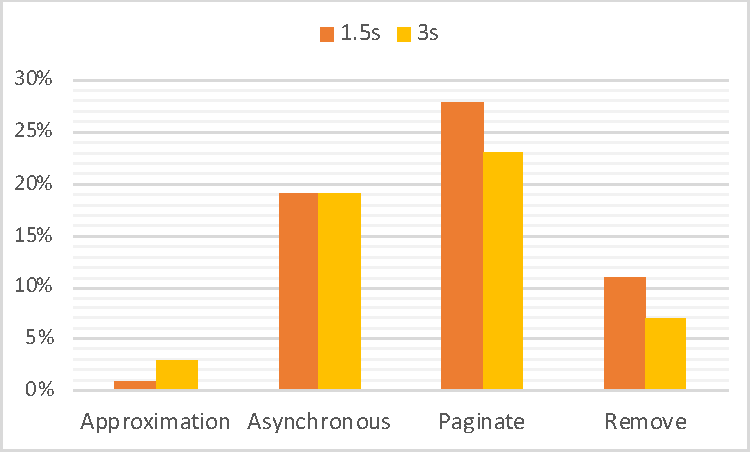
\includegraphics[width=0.8\columnwidth]{figs/preference.pdf}
    \caption{How much better do users like New pages?}
    \label{fig:userstudy_diff}
\end{figure}
\begin{figure}[h]
    \centering
    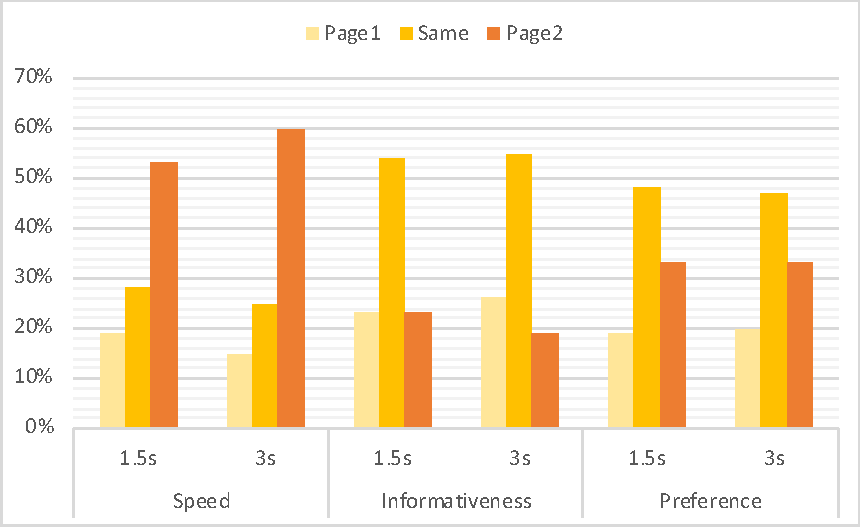
\includegraphics[width=0.8\columnwidth]{figs/user-study.pdf}
    \caption{How people prefer the pages?}
    \label{fig:userstudy}
\end{figure}
\fi

\subsubsection{User study results}
A summary of the user study results is shown in Table \ref{tab:userstudy_diff}, and the questionnaire and raw data are available on Panorama webpage \cite{userstudydata}.
%, there are always some participants who think Base is better, and some think New is better, and some think two versions are similar. \alvin{just say the results are mixed?}
In this table, we show the percentage of users who
think New is better minus those who think Base is better,
which we refer to as the {\it net} benefit of the new design, for every type of refactoring and every
question (Performance, Functionality, and Overall).
Users are given the two pages in random order, and are not aware of the view-design difference between the two pages in advance.

A short answer to our research question is ``Yes''. In fact, for all type
of view-changing optimization, users think the New design is {\it not worse}
than the Base design. Particularly, for {\it asynchronous} loading,
{\it pagination}, and {\it removal}, the new designs clearly win more users
than the baseline designs.

In terms of performance, the net win for the New design is clear. Many users
indeed notice the 1.5-second difference in the page-load time. In 10 out of 12 cases, \alvin{show \%?}
the New design has a net positive benefit on more than 30\% of the participants.

In terms of functionality, the results are quite interesting. For 
{\it approximation} and {\it pagination}, many users did notice the
content difference, leading to the Base design winning about 10\% of users.
However, for {\it asynchronous} loading and content {\it removal}, surprisingly,
many users neither notice the content difference nor think New design delivers worse contents. It could be that removing contents made the page cleaner to some users. For example, after removing the sidebar in Tracks \alvin{in Tracks? (if tracks is the app name)} (Tr5 in Table \ref{tab:dbsize} \alvin{I can't find case 11 in that table?}), some participants like it because ``Adding the sidebar makes scrolling harder.'' 

In terms of overall perception, the New design has a {\bf net win}.
Among the four types of optimizations, paginations and asynchronous loading
are the most appealing to users, while approximation is the least appealing.

We also conducted another set of user study with another 100 participants,
where we use an even larger (2-10$\times$) database size \alvin{how large?} \junwen{The size get differntly larger for different cases, some are 10 times, some are 2 times, some are 2.5 times} and hence make the page-load time
differences between New design and Base design even bigger (3 seconds).
We do observe that more participants noticed the performance advantage
of the New design. However, we also observe that the overall perception
only goes up a little bit more for the New design. We skip the details for
the space constraints.



\begin{table}[]

\centering
\caption{Net user perception enhancement by New design\\ (\% users 
who prefer New   $-$ \% users who prefer Base )}
\label{tab:userstudy_diff}
\begin{tabular}{@{}lrrrr@{}}
\toprule
                                & Approximation & Asynch & Paginate & Removal  \\ \midrule
Performance       & 23.50\%       & 31.00\%      & 45.00\%  & 35.50\% \\ 
%                             & 3s   & 35.50\%       & 42.00\%      & 45.50\%  & 58.00\% \\ \midrule
Functionality  & -7.50\%       & 17.50\%      & -13.00\% & 5.50\%  \\ 
 %                            & 3s   & -10.50\%       & 10.50\%      & -24.50\%  & -3.00\% \\ \midrule
Overall   & 1.00\%        & 18.50\%      & 28.00\%  & 10.50\% \\  
 %                            & 3s   & 2.50\%        & 19.00\%      & 23.00\%  & 7.00\%  \\ 
 \bottomrule
\end{tabular}
 \vspace{-0.2in}
\end{table}


\iffalse
\begin{table}[]
\centering				
\caption{User Study Result: Why prefers a web page?}
\label{tab:codebook}	\begin{tabular}{@{}clrm{3.5cm}@{}}
\toprule
                                            & Reason        & Num & Example                                           \\ \midrule
\multirow{3}{*}[-10pt]{Page 1}                     & Informative  & 125 & p1 has more  information.             \\ \cmidrule(l){2-4} 
                                            & Faster        & 37  & p1 loads fast.                                \\ \cmidrule(l){2-4} 
                                            & Display Style & 59  &  not paginating  is helpful. \\ \midrule
\multicolumn{1}{l}{\multirow{3}{*}[-10pt]{Page 2}} & Informative   & 83  & p2 has  more information.             \\ \cmidrule(l){2-4} 
\multicolumn{1}{l}{}                        & Faster        & 215 & p2 loads much faster.                         \\ \cmidrule(l){2-4} 
\multicolumn{1}{l}{}                        & Display Style & 168 & I like paginating.         \\ \bottomrule
\end{tabular}
\end{table}
\fi
\iffalse
\emph{Discussion.} The baseline page load time greatly affects people's attitude towards end-to-end time consumption. It's because of the non-uniform Internet status and human sense of time. In addition, longer loading time is, the more information on web-page the participant is expecting. During the experiment, we also found that participants have a strong preference towards pagination. Some of them think pagination is a clean UI design, while the others regard it as an obstacle to searching.
%[does the base line page-load time affect people's reaction?] [Does the users' reaction differ for different types of view-changes?]

\fi


\vspace{-0.05in}
\subsection{RQ4: how accurate is the \Tool estimator?}
We use the web page shown in Figure \ref{fig:heatmap} as a case study.
15 HTML tags on this page render dynamically generated contents.
With 200 database records, dynamic profiling shows that
the story tag is the top performance bottleneck, followed by the guideline
tag and then the message-count the cheapest. When the workload increases to
2000 and 20000 records, dynamic profiling shows that the guideline
tag is the top bottleneck, followed by the story tag. These results match
the performance gains we can get by optimizing these three tags: 
using 20000 records, asynchronously
loading or removing the guideline text can reduce the page end-to-end 
load time by more than 1 second; 
paginating the story-tag can speed up the page load time
by about 100 milliseconds; approximating the message count does not change page load time.

The static mode of \Tool estimator can indeed predict performance bottleneck
without running the application --- the guideline text gets the
highest complexity score (5) among all 15 tags, followed by the story tag (4), and then the
message-count tag (3), with the remaining 12 tags
getting 0 points.


\iffalse
\begin{table}[]
\centering
\caption{Performance cost ranking (static vs dynamic)}
\label{tab:cons1}
\begin{tabular}{@{}lrrrrrrr@{}}
\toprule
 & \multicolumn{2}{l}{200} & \multicolumn{2}{l}{2000} & \multicolumn{2}{l}{20000} & \multicolumn{1}{l}{static} \\ \midrule
guideline & \cellcolor[HTML]{C0C0C0}2 & 2 & \cellcolor[HTML]{C0C0C0}1 & 1 & \cellcolor[HTML]{C0C0C0}1 & 1 & 1 \\ \midrule
tags & \cellcolor[HTML]{C0C0C0}1 & 1 & \cellcolor[HTML]{C0C0C0}2 & 2 & \cellcolor[HTML]{C0C0C0}2 & 2 & 2 \\ \midrule
msg\_count & \cellcolor[HTML]{C0C0C0}3 & 3 & \cellcolor[HTML]{C0C0C0}3 & 3 & \cellcolor[HTML]{C0C0C0}3 & 3 & 3 \\ \bottomrule
\end{tabular}
\end{table}
\fi


%%%%%%COMMENT OUT%%%%
\begin{comment}

\begin{table}[]
\centering
{\small					
\caption{User Study Result: How people prefer the pages?}
\label{tab:userstudy}	
\begin{tabular}{@{}llrrrr@{}}
\toprule
 &  & \multicolumn{1}{l}{page1} & \multicolumn{1}{l}{same} & \multicolumn{1}{l}{page2} & \multicolumn{1}{l}{diff} \\ \midrule
Speed & 1.5s & 19.00\% & 28.25\% & 52.75\% & 33.75\% \\ \midrule
 & 3s & 15.13\% & 24.50\% & 60.38\% & 45.25\% \\ \midrule
Info&1.5s & 22.63\% & 54.13\% & 23.25\% & 0.63\% \\ \midrule
 & 3s & 26.00\% & 54.88\% & 19.13\% & -6.88\% \\ \midrule
Prefer & 1.5s & 18.88\% & 47.75\% & 33.38\% & 14.50\% \\ \midrule
 & 3s & 20.00\% & 47.13\% & 32.88\% & 12.88\% \\ \bottomrule
\end{tabular}
}
\end{table}

\end{comment}

\subsection{Threats to validity}
Threats to the validity of our work could come from multiple
sources. 
\textbf{Internal Validity}: The HTML tags that are dynamically generated through JavaScript can not be detected or analyzed by \Tool. \textbf{External Validity}: The 12 applications in our benchmark suite may not represent all real-world applications; The synthesized databases may not represent real-world workloads; The machine and network settings of our profiling may differ from real users’ setting; the 100 participants of our user-study from MTurk may not represent all real-world users. Overall, we have tried our best to conduct an unbiased study.





% \section{Related work}
% Recent work uses
ORM-aware static analysis to detect performance anti-patterns \cite{yang2018powerstation, chen2016finding0} and data constraint problems \cite{yang2020managing} in database-backed web applications. They did not look at
schema changes and are orthogonal to our work. 
%https://dl.acm.org/doi/pdf/10.1145/3314221.3314588 
%Our study does not consider constraint change since it's well studied in our previous work~\cite{yang2020managing}.
\Tool is motivated by recent work \cite{wang2017verifying, wang2019synthesizing} about schema changes in web applications, but is different from
them as discussed earlier. Specifically, MIGRATOR
\cite{wang2019synthesizing} analyzes schema changes in SQL and synthesizes SQL queries,
while \Tool looks at Rails (Ruby) and Django (Python) application; MIGRATOR handles
renaming changes and structure changes like moving a column from one table to another,
while \Tool handles all the changes in Table \ref{tab:overview}.

\section{Conclusion}

\label{sec:con}
It is increasingly challenging to develop web applications that can deliver both good functionality and desired performance. We present \Tool, a tool that
helps web developers explore the performance-functionality trade-off space
in their web application design. The \Tool estimator provides developers 
with data-processing cost information for every HTML tag that renders
dynamically generated data, while the \Tool optimizer identifies and automates
view-changing refactoring that can greatly improve performance.
The \Tool interface integrates estimator and optimizer together to enable effective web application design. 



\chapter{Managing data constraints in database-backed web applications}
\section{Overview}
In this chapter, we aim to answer four key research questions about real-world database-backed
web applications, as listed in Table~\ref{table:highlight} by comprehensively
studying the source code, the commit history, and the issue-tracking system of 12 popular Ruby on Rails applications that represent 6 most common web-application categories. 

\begin{table}[h]
\centering
\caption{Highlight results of our study} 
\footnotesize{\textmd{(*: all the identified issues are in latest versions of these applications)}}
 \setlength{\tabcolsep}{1pt} 
\label{table:highlight}
\resizebox{0.7\columnwidth}{!}{
\begin{tabular}{@{}ll@{}}
\toprule
\multicolumn{2}{c}{\bf RQ1: How are constraints specified in one software version?}\\
 
{How}    &  2.1 per 100 LoC            \\
%\cmidrule(l){2-2} 
Many?              &  1.4 per 1 data field       \\ 
% \cmidrule(l){2-2} 
                              & 77\% of data fields have constraints\\
%                              \midrule
\multirow{2}{*}{Where?}       & 76\% in DB; 23\% in application; 1\% in front-end     \\  
%\cmidrule(l){2-2} 
                              & 24\% of application constraints are missing in DB\\
                             
                              \midrule
\multicolumn{2}{c}{\bf RQ2: How are constraints specified across versions?}\\
 
                                & 49\% of versions contain constraint changes  \\
                                & $>$ 25\% of changes tighten constraints on existing data fields\\
                                
\midrule                                 
\multicolumn{2}{c}{\bf RQ3: What led to real-world constraint problems?}\\ 
 
Where       & 21\% of \numissues studied issues\\
What        & 51\% of \numissues studied issues\\
When        & 10\% of \numissues studied issues\\
How         & 18\% of \numissues studied issues\\
\midrule 
\multicolumn{2}{c}{\bf RQ4: Can we identify constraint problems in latest version?}\\
Where       & 1000+ string fields have length constraints in DB but not in app. \\
            & 200+ fields forbidden to be {\tt null} in app. but {\tt null} by default in DB\\  
            & 88 fields required to be unique in app. but not so in DB\\
            & 57 in(ex)clusion constraints specified in app. but missed in DB\\
            & 133 conflicting length/numericality constraints between app. and DB\\ 
What        & 19 incorrect case-sensitivity constraints identified\\
How         & 2 missing error-message problems identified\\
            & API default error-message enhancement preferred in user study\\
\bottomrule
\end{tabular}
}

\end{table}

{For RQ1}, we wrote scripts to collect and compare constraints expressed in various components of the latest versions of the 12 applications. We found that about three-quarter of all data fields are associated with constraints. In total, there are hundreds to over 
one thousand constraints explicitly specified in 
each application, averaging 1.1--3.6 constraints
specified per 100 lines of code. Data presence and data length are the two most common types of constraints,
while complicated constraints like the relationship among multiple fields also exist. 
We also found
that hundreds to thousands of constraints specified in the
database are missing in the application source code, and vice versa, 
which can lead to maintenance, functionality,
and performance problems.
The details are presented in Section \ref{sec:wherewhat}.


{For RQ2}, we checked how data constraints change throughout the applications' development history. 
We found that about 32\% of all the code changes related to data constraints is about adding new constraints or changing existing ones on data fields that have already existed in software. These changes, regardless of whether they are due to developers' earlier mistakes or warranted by new code features, can easily lead to upgrade and usage problems for data that already exists in the database.
The details are in Section \ref{sec:evolve}.
 
{For RQ3}, we thoroughly investigated \numissues real-world issues that are related to data constraints. We categorize them into four major anti-patterns:
(1) inconsistency of constraints specified at different places, which we refer to as the {\it Where} anti-pattern;
(2) inconsistency between constraint specification and actual data usage in the application, which we refer to as the {\it What} anti-pattern;
(3) inconsistency between data/constraints between different application versions,which we refer to as the {\it When} anti-pattern;
and (4) problems with how constraint-checking results are
delivered (i.e., unclear or missing error messages), which
we refer to as the {\it How} anti-pattern. These four anti-patterns are all common and difficult to avoid by developers; they led to a variety of failures such as web-page crashes, silent failures, software-upgrade failures, poor user experience, etc.   
The details are presented in Section \ref{sec:causes}.

{For RQ4}, we developed tools that automatically identify many
data-constraint problems in the latest versions of these 12 applications, as highlighted in Table \ref{table:highlight}.  
We found around 2,000
``Where'' problems, including many fields
that have important constraints specified in the database
but not in the application or vice versa, as well as
over 100 fields that have length or numericality (i.e., numerical type and value range)
constraints specified in both the database and the application, 
but the constraints conflict with each other. We also found 19
issues in which the field is associated with case-insensitive uniqueness constraints, 
but are used by the application in a case-sensitive way
(the ``What'' anti-pattern), as well as
two problems related to missing error messages (the ``How'' anti-pattern).
We manually checked around 200 randomly sampled problems and found a low
false positive rate (0--10\%) across different types of checks. 
Not to overwhelm application developers, 
we reported \numreportedissues of these problems to them, covering all problem categories. We received \numconfirmedissues confirmation from the developers (no feedback yet to the other \numunconfirmedissues reports), among which our proposed patches for \nummergedissues of those problems have already been merged into their applications or included in the next major release. 
 %\shan{fill in xx}

We also developed a Ruby library that improves the default error messages of
five Rails constraint-checking APIs. We performed a user study with results showing that web users overwhelmingly prefer our enhancement.
The details are presented in Section \ref{sec:solution}.
 
Overall, this paper presents the first in-depth study of data constraint problems in web applications.
Our study provides motivations and guidelines for future research to help developers
better manage data constraints.   We have prepared
a detailed replication package for the data-constraint-issue study and the data-constraint checking tools  in this paper. This package is available on the webpage of our open-source Hyperloop project~\cite{hyperloop}, a
project that aims to solve database-related problems
in ORM applications.


\section{Methodology}
\label{sec:meth}
\subsection{Application selection}
 There are many ORM frameworks available (e.g., Ruby on Rails, Django, Hibernate, etc.). Among them, Rails is the most popular on Github. 
Thus, we studied 12
open-source Ruby on Rails applications, including the top two most popular Ruby applications from six major categories of web applications on GitHub: Discourse (Ds) and Lobster (Lo) are forums; Gitlab (Gi) and Redmine (Re) are collaboration pplications; Spree (Sp) and Ror ecommerce (Ro) are Ecommerce applications; Fulcrum (Fu) and Tracks (Tr) are Task-management applications; Diaspora (Da) and Onebody (On) are social network applications; OpenStreetmap (OS) and FallingFruit (FF) are map applications. All of them have been actively developed for years, with hundreds to tens of hundreds of code commits. 

\subsection{Issue selection}
\begin{table} 
% \setlength{\tabcolsep}{1 pt}  
\centering 
\caption{\# of data-constraint issues in our study and the total \# of issues in the issue-tracking system}
%\footnotesize
% @{\hspace{0.1in}}r@{\hspace{0.1in}}r@{\hspace{0.1in}}r@{\hspace{0.1in}}r@{\hspace{0.1in}}r@{\hspace{0.1in}}r@{\hspace{0.1in}}r@{\hspace{0.1in}}r@{\hspace{0.1in}}r@{\hspace{0.1in}}r@{\hspace{0.1in}}r@{\hspace{0.1in}}r@{\hspace{0.1in}}
% \resizebox{0.9\columnwidth}{!}{
\begin{tabular}{lrrrrrrrrrrrr}
\toprule
 & Ds & Lo & Gi & Re & Sp & Ro & Fu & Tr & Da & On & FF & OS\\
\midrule
Studied &14 & 1 & 16 & 30 & 31 & 2 & 1 & 1 & 11 & 5 & 0 & 2\\
\midrule
Total &4607 & 220 & 18038 & 12117 & 4805 & 114 &158 &1470 &3206 & 400 & 17 & 650\\
\bottomrule
\end{tabular}
% }
\label{table:issueapp0}
% \vspace{-0.2in}
\end{table}

Section~\ref{sec:causes} studies the root causes and symptoms of real-world data constraint problems using
\numissuescon reports sampled from the above 12 applications' issue-tracking systems. For the 9 applications that have medium-size
issue databases (i.e., 100--5000 total reports), we randomly sampled 100 reports for each. For Redmine and Gitlab, which have more than 10,000 reports, we randomly sampled 200 reports for each. For FallingFruit, which only has 17 reports, we took all of them. Among the resulting 1317 sampled reports, we manually
checked all the reports that contain keywords like ``data format,'' ``data inconsistency,'' ``data constraint,'' ``format change,'' ``format conflict,'' etc. We finally obtained
\numissuescon reports that are truly related to data constraints, as shown in \tabref{issueapp0}.  


\section{Constraints in one version}
\label{sec:wherewhat}

To understand how many constraints are  specified in  software, where they are located, and what they are about, we wrote scripts to extract data constraints from the latest version of 
the 12 applications described in Section \ref{sec:meth}. Our scripts obtain a web application's Abstract Syntax Tree, check which Ruby validation APIs and migration APIs are used, and analyze their parameters.

In this paper, our script covers all types of constraints listed
in Table \ref{table:constraintdeftax} except for   
Custom sanity checks and raw SQL constraints. Both are rarely used in these
applications (e.g., raw SQL constraints are only specified in fewer than
30 times across all 12 applications). Note that, when we report inconsistency
or missing constraints, 
we manually check to make sure the inconsistency/missing constraint is not caused by
our script not covering these two types of constraints.

%Since it is impractical to automatically extract all custom sanity checks, we randomly sample some of the sanity checks and manually analyze them at the end of this section.

\subsection{How many constraints are there?}

\begin{table}
%\setlength{\tabcolsep}{1.2pt} 
\centering
\caption{\# Data constraints in web applications} 
\resizebox{0.7\columnwidth}{!}{
\begin{tabular}{lrrrrrrrrrrrr}

\toprule
 & Ds   & Lo  & Gi   & Re  & Sp  & Ro  & Fu & Tr  & Da  & On  & FF  & OS  \\
\midrule
DB   & 1403 & 137 & 1582 & 437 & 346 & 378 & 34 & 108 & 361 & 345 & 159 & 242 \\
App  & 165  & 33  & 496  & 220 & 132 & 219 & 13 & 30  & 116 & 82  & 17  & 176 \\
HTML & 0    & 2   & 18   & 32  & 0   & 0   & 0  & 2   & 1   & 11  & 0   & 0   \\
\midrule
Total  & 1568 & 172 & 2096 & 689 & 478 & 597 & 47 & 140 & 478 & 438 & 176 & 418\\
\midrule
\midrule 
LoC  & 62k & 11k & 122k & 35k & 31k & 17k & 1.7k & 13k & 21k & 14k & 7.8k & 14k
 \\
\midrule
\midrule 
\#Col   & 1180 & 150  & 1384 & 338  & 456  & 384  & 53   & 107  & 510  & 268  & 171  & 228  \\
\#Col$_\text{C}$ & 882  & 104  & 1140 & 297  & 312  & 272  & 32   & 82   & 348  & 228  & 146  & 174  \\
\%Col$_\text{C}$ & 75\% & 69\% & 82\% & 88\% & 68\% & 71\% & 60\% & 77\% & 68\% & 85\% & 85\% & 76\%\\
\bottomrule
\end{tabular}
}

{\footnotesize LoC: Lines of code. \#Col: number of data columns stored in the database. \\
\#Col$_\text{C}$.: number of columns associated with constraints.
Custom sanity check not considered.
}
\label{table:latestconstraintnum}
\end{table}

As shown in Table \ref{table:latestconstraintnum}, there are many constraints in these applications. 
%Naturally, the larger the software is and the more data columns the software contains, the more constraints are specified. 
Across all applications, 60\% - 88\% of data columns are associated with constraints and there exists 1.1 to 3.6 constraint specifications for every 100 lines of code.

\paragraph{\bf Summary} Data constraint specification widely exists in all types of web applications. Their consistency, maintenance, and handling affect the majority of the application data.


\subsection{Where are the constraints?}
\label{sec:one_where}

As shown in Table \ref{table:latestconstraintnum}, DB constraints are the most common, contributing to
58--90\% of all the constraints. Application constraints contribute 10--42\%, while front-end constraints are few.   
It is surprising that the number of DB constraints differs significantly compared to
application constraints, as both are supposed to be applied to a given piece of persistent data (Section \ref{sec:back_constraints}). Furthermore, inconsistencies
between them can lead to application crashes as in the example shown in Figure~\ref{fig:crossstack}. 
This led to the next few study items.

\paragraph{\bf What DB constraints are missing in applications?}
Table~\ref{table:dbpresentmodelmissingbreakdown} examines over
4,000 DB constraints that are missing in applications.

Alarmingly, about one quarter of these missing constraints (more than 1,000 in total)  involve string/text
data where developers did not specify any length constraints in the application, 
yet length constraints are imposed by the DB.
For example, 
whenever creating a table column of type ``string'' using Rails migration API, by default, Rails framework forces a length constraint of 255-character in the database, yet many of these string fields have no length constraints specified through application validation functions.
%Another example is MySQL has a default length constraint (no more than 65535 characters) on column of type ``text'', and applications often do not have the corresponding length limit. 
%when MySQL is the DB engine, all {\it text} fields 
%have 65535-character length constraint by default, and
%all {\it string} fields have 255-character length constraint
%by default set by the Rails migration API that adds or removes tables, columns, or entries \alvin{what's the migration api for?} \junwen{migration api is used to create db or alter db, they will be translated to sql queries to create/alter table}
%regardless of the databaseengine type.\junwen{Before Rails 4, 255 is for every engine, after Rails 4, 255 is only for MySQL} 
This mismatch could lead to severe problems: if a user tries to submit a long
paragraph/article in such a seemingly limitless field, his application will crash due to a failed {\tt INSERT} query, as shown in Figure~\ref{fig:crossstack}. In fact, we found many real-world issues reporting this problem (Sec.~\ref{subsec:where}), ultimately leading to developers adding the corresponding constraints in the application layer.

About 2\% of the missing constraints, 101 in total across the 12 applications, are associated with data fields that do not exist in the application.
Some of them are updated and read through 
external scripts, but never through the web application; 
others are deprecated fields that have already been removed
from the application but not dropped yet from the DB. 
Although this does not lead to immediate software misbehavior, 
these cases reflect challenges in
data maintenance and could cause functionality problems in the future. In addition,
they cause performance problems as the database needs to maintain deprecated data.

About one third of the missing constraints are automatically satisfied by Rails or the DB and are hence benign. This includes presence and numericality constraints associated with foreign-key fields (``ForeignKey''): 
foreign key fields are automatically generated
by Rails and satisfy presence
and numericality constraints in the DB. Meanwhile, there are also constraints that are guaranteed by the DB (``SelfSatisfied''), like presence constraints guaranteed by non-null default values specified in the DB, uniqueness constraints guaranteed by an auto-increment property in the DB, etc.

\begin{table}
\centering
\caption{\# Constraints in DB but not in Application} 
\setlength{\tabcolsep}{2pt}  
\resizebox{0.7\columnwidth}{!}{
\begin{tabular}{lrrrrrrrrrrrrr}

\toprule
& Ds   & Lo  & Gi   & Re  & Sp  & Ro  & Fu & Tr  & Da  & On  & FF  & OS & All \\
\midrule
StrLength & 243 & 21 & 406 & 49 & 182 & 47 & 18 & 21 & 101 & 69 & 74 & 28 & 1259 (28\%) \\ \midrule
AbsentData & 21 & 0 & 40 & 2 & 2 & 2 & 2 & 1 & 22 & 7 & 2 & 0 & 101 (2\%) \\ 
\midrule
ForeignKey & 266 & 31 & 271 & 82 & 27 & 99 & 7 & 27 & 61 & 91 & 16 & 30 & 1008 (22\%) \\ \midrule
SelfSatisfied & 192 & 16 & 161 & 84 & 28 & 9 & 2 & 18 & 3 & 20 & 8 & 31 & 572 (13\%) \\ \midrule
Others   & 446 & 39 & 429 & 126 & 77 & 89 & 2 & 29 & 143 & 82 & 26 & 64 & 1552 (35\%) \\
\bottomrule
\end{tabular}
}
\label{table:dbpresentmodelmissingbreakdown}
\end{table}

\begin{table}
\centering
\setlength{\tabcolsep}{1.5pt}  
\caption{\# Constraints in Application but not in DB }
{\textmd{(only
built-in validation constraints are listed)}}
 
\resizebox{0.7\columnwidth}{!}{
\begin{tabular}{lrrrrrrrrrrrrr}

\toprule
& Ds   & Lo  & Gi   & Re  & Sp  & Ro  & Fu & Tr  & Da  & On  & FF  & OS & All \\
\midrule
Presence & 8 & 5 & 37 & 15 & 38 & 49 & 5 & 5 & 34 & 3 & 1 & 9 & 209 (51\%) \\ \midrule
Unique & 3 & 1 & 12 & 18 & 19 & 5 & 0 & 4 & 16 & 1 & 0 & 9 & 88 (21\%) \\ 
\midrule
Inclusion/Exclusion & 7 & 1 & 13 & 11 & 2 & 0 & 2 & 0 & 7 & 5 & 0 & 9 & 57 (14\%) \\ \midrule
RegEx & 8 & 5 & 10 & 7 & 0 & 9 & 0 & 0 & 11 & 4 & 0 & 3 & 57 (14\%) \\ \midrule
%Other   & 15 & 2 & 3 & 9 & 13 & 1 & 0 & 0 & 3 & 0 & 2 & 10 & 58 (11\%) \\
Numeric   & 0 & 0 & 0 & 0 & 0 & 1 & 0 & 0 & 0 & 0 & 0 & 0 & 1 (0.2\%) \\ 
\bottomrule
\end{tabular}
}
\label{table:modelpresentdbmissingbreakdown}
\end{table}

The remaining one third of the constraints ("other") are difficult to analyze automatically. Based on our manual sampling and checking, most  
are already satisfied by how the application processes and generates corresponding data fields. 
Although they do not cause problems currently, developers should nonetheless be informed about them, so that code changes can be tested
against these constraints to prevent regression failures. 

\underline{\it False-positive analysis}\ \ Besides the ``Others'' row in Table \ref{table:dbpresentmodelmissingbreakdown},  
the other 4 rows are counted by our static-checking script. 
To check the accuracy of our script,
we randomly examined 102 cases from these 4 rows.
Among these cases, we found 7 false positives: 5 are not
DB constraints but are mistakenly identified due to syntax not handled by our script; 2 ``StrLength'' cases  
actually belong to ``Others,'' as the length requirement is guaranteed
by application semantics. These 102 cases include 58 ``StrLength''
cases, among which 5 are false positives --- 3 are not
DB constraints and 2 belong to ``Others''. %\junwen{Utsav, can you update the value here.}

\paragraph{\bf Which application constraints are not in database?}
Nearly 25\% of the constraints specified through application validation are missing in the DB.  
Table \ref{table:modelpresentdbmissingbreakdown}
breaks down the ones specified through built-in validation 
functions based on the constraint type
(412 in total). 
These missing constraints allow users to directly
change persistent data using SQL queries in ways that are disallowed by the application, causing functionality or even security problems.\footnote{It is common that database administrators directly change database data using queries and scripts, bypassing the application server.} Furthermore, some of these missing constraints represent missed query optimization opportunities, such as improving cardinality estimation in query plan generation using such constraints~\cite{lohmanBlog}.

About half of these missing constraints
are presence constraints. That is, a field $f$ is required to be non-null in the application, but is not required so in the DB --- their default values are ironically set to be null in the DB. 
When users or administrators directly insert records into the DB without specifying the value
for a field $f$, the DB would accept these records and put null into $f$. 
Subsequently, when such records are retrieved and used in the application that 
assumes all $f$ to be non-null, software failures could occur.

Another category of missing constraints that can easily cause problems are uniqueness constraints. Without being
specified in the DB, a uniqueness constraint often {\bf cannot} be guaranteed by the application \cite{perilsofuniqueness,uniquenessrb}: 
web users could make concurrent update requests that save duplicate values into the DB, violating the uniqueness constraint and causing software failures and maintenance challenges. 
%(the discovery and cleanup of bad data).
%\utsav{Rails uses transactions on save by default, but I think the isolation level, at least for Postgres, is READ COMMITTED which may not prevent against this. Anyway it may happen infrequently in practice, but there are warnings about this in the rails documentation https://github.com/rails/rails/blob/master/activerecord/lib/active\_record/validations/uniqueness.rb\#L165, and in blog posts: https://thoughtbot.com/blog/the-perils-of-uniqueness-validations}


Regular expression and inclusion/exclusion constraints are rarely found in the DB layer. While these can be enforced via procedures or {\tt ENUM} types, they are not natively supported by the Rails DB migration APIs and have to be explicitly specified via SQL, which might be a reason why they tend to be missed in the DB.
Inclusion/exclusion 
constraints limit the value of a field to a small set of
constants and would be very useful in avoiding data corruption, saving storage space, and improving database performance (e.g.,
through DB selectivity optimization) if they are present.

The single numeric constraint in Table \ref{table:modelpresentdbmissingbreakdown} is a ``phone number'' field that is
specified to be numeric in application but stored as a ``string'' in the database.

\underline{\it False-positive analysis}
 We randomly sampled
and examined 10 cases from each of the 4 main categories in Table \ref{table:modelpresentdbmissingbreakdown} (Presence, Unique,
In/Ex-clusion, RegEx).  
3 out of the 40 sampled cases are false positives 
(2, 0, 0, 1 in the 4 categories, respectively)---syntax corner cases caused our script to identify 1 spurious presence constraint, and the remaining 2 are related to conditional constraints.

\paragraph{\bf Summary} Hundreds and thousands of database constraints do not exist
in application, and vice versa. The majority of these discrepancies can actually
lead to bad user experience (missing string length constraints),   
database maintenance challenges (data fields that are no longer used in the application),
code maintenance challenges (constraints implicitly guaranteed by the application logic),
data corruptions, software failures, or sub-optimal database performance (missing DB constraints). They can be avoided by implementing constraints in the application and as SQL constraints in the database. However, in practice inconsistencies are likely inevitable if we only rely on developers' manual effort.
It would be helpful to develop automated techniques that coordinate
database and application constraints.

\subsection{What types of constraints are there?} 
\paragraph{\bf Standard types}
Table~\ref{table:apibreakdown} shows the most popular constraint types among all front-end, application built-in validation, and DB constraints. 
The top 2 most popular types are consistently presence and length.
%The much smaller number of Numericality constraints in Application is due to the fact that numericality constraints for foreign-key fields are implicitly enforced by Rails and hence not specified in application.
%None of the 86 Inclusion application constraints exist in the DB, as discussed earlier.


\begin{table}[]
\caption{Top 5 popular types of different layer}
\centering
\resizebox{0.7\columnwidth}{!}{
\begin{tabular}{@{}llllll@{}}
\toprule
DB  &   Presence & Length &  Numericality&  Uniqueness   & -         \\ \midrule
 &  1822 (32.9\%)        & 1784 (32.3\%)      & 1650 (29.8\%)              & 276 (5.0\%)              & -         \\ \midrule
App. & Presence & Length & Uniqueness   & Numericality & Inclusion \\ \midrule
 & 888 (52.3\%)         & 218 (12.8\%)       & 209 (12.3\%)             & 101 (5.9\%)              & 67 (3.9\%)       \\ \midrule
HTML  & Presence & Length & Format       & -            & -         \\ \midrule
    &52 (78.8\%)          & 11 (16.7\%)        & 3 (4.5\%)         &            -  &      -     \\ %\midrule
%Sum   & Presence & Length & Numericality & Uniqueness   & Inclusion \\ \midrule
%      & 2822     & 1780   & 1492         & 414          & 77        \\ 
\bottomrule
\end{tabular}
}
\label{table:apibreakdown}
\end{table}


\paragraph{\bf Custom validation constraint types}
Custom validation functions are used much less often than built-in ones,
but are not rare, contributing about 5\% to slightly over 25\% of all application
validation functions across the 12 applications (avg. 18\% across all apps). 
%To understand what types of custom constraints are specified, 
We randomly sampled 50 custom validation functions
and found that more than half of them are used to check multiple fields at the same time (27 out of 50), like the function {\tt presence\_of\_content} in the
{\tt StatusMessage} model from {\tt Diaspora}, which requires that at least one of the fields {\tt text} or {\tt photos} be non-empty. 
%In some cases (11 out of 50), the condition checking involves data in DB tables used by the application but not directly associated with the model, or data from the application configuration. \shan{this table is not managed by the web application?}\utsav{Tried to clarify} 
These custom validations seldom have corresponding constraints in DB --- only 4 out of the 50 we sampled exist in DB.  

\iffalse 
\begin{table}[h]
\caption{\# Custom validation constraints (sample size: 50)}
\setlength{\tabcolsep}{2pt}  
\footnotesize
%@{\hspace{0.3in}}r@{\hspace{0.3in}}r@{\hspace{0.3in}}r@{\hspace{0.3in}}r@{\hspace{0.3in}
\resizebox{0.9\columnwidth}{!}{
\begin{tabular}{rrrr}
\toprule
 Multi-field & Pre-processing & External data & Other \\
\midrule
27 & 6 & 11 & 16 \\
\bottomrule
\end{tabular}
}
\label{table:custommethodmulti}
\label{table:issueapp}

{\footnotesize Note that some custom validators contain multiple functionalities.}
\end{table}
\fi 




\iffalse
\begin{figure}[h] 
    \centering
    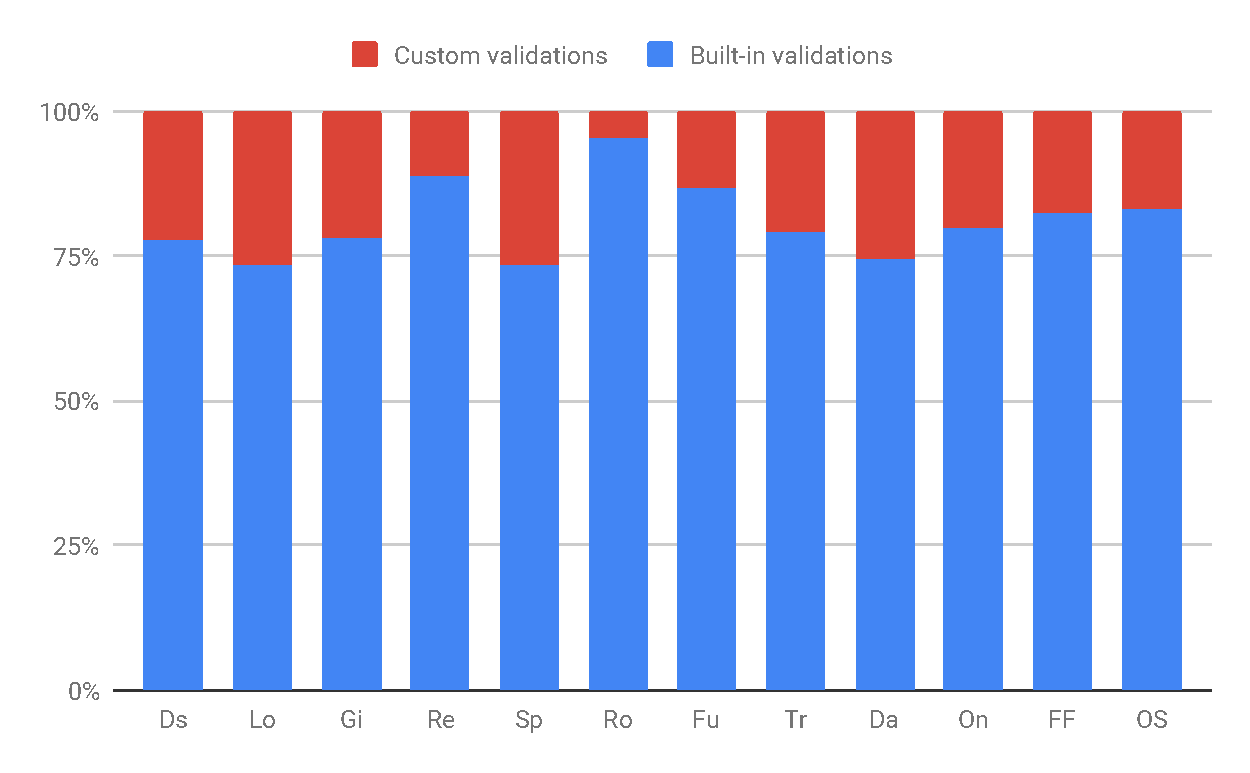
\includegraphics[width=\columnwidth]{figs/custom-vs-builtin-validations.pdf}
    \caption{Breakdown of \# of custom vs. built-in validations in model layer
\\  \junwen{change to a table?}
}
    \label{fig:model-breakdown}
\end{figure}
\fi 


\paragraph{\bf Custom sanity check types}

We also sampled 20 sanity checks on input parameters from the controller code of 5 applications.
%\shan{are these in one application or multiple? }
Among these 20 checks, the majority (17) are indeed checking inputs  that are related to persistent
data stored in the DB. Among these 17, 5 are about
data constraints, including presence and inclusion constraints, 
while the others are related to conditional data update/re-processing.
 Among these 5 constraints, only 1 is specified
in an application validation function and none exists in the DB.
%this 1 case is an inclusion constraint  

\iffalse 
\begin{table}[h]
\caption{\# Param sanity checking w/ category (sample size: 20)}
\footnotesize
\begin{tabular}{@{\hspace{0.1in}}r@{\hspace{0.2in}}r@{\hspace{0.2in}}r@{\hspace{0.2in}}r@{\hspace{0.1in}}}
\toprule
 Stored in DB & Constraint & Constrained in model & Constrained in DB\\
\midrule
17 & 5 & 1 & 0\\
\bottomrule
\end{tabular}
\label{table:nonapiconstraint}
\label{table:issueapp}

\end{table}
\fi 

\paragraph{\bf Summary} Although simple constraints like presence, length,
and numericality are the most common, more complicated constraints, such as those
involving multiple fields, are also widely used. Most of the
custom constraints are missing from the DB, while constraints reflected by sanity checks are often missing in both the application and DB. 
Future research that can automatically
reason about custom sanity checks and custom validation 
functions
%, which will likely require symbolic code evaluation,
can greatly help to identify and add missing constraints.

\section{Constraints   across versions}
\label{sec:evolve}

The software maintenance task for web applications comes with the
extra burden of database  maintenance, including both data format changes, 
like adding
or deleting a table column, and data constraint changes, like
changing the length requirement of a password field.
In this section, we study how constraints evolve across versions
and the related data-maintenance challenges.

\paragraph{\bf How often do constraint-related changes occur?} 
% As shown in  Table~\ref{table:firstlatestcomparison}, 
We first checked the first commit of each application, and found {\it no}
data constraints in all but 3 applications (Ds, Lo, FF).
For all applications, the majority of the constraints were added in later commits.

%We then check how often data constraints change across versions. 
%Different applications release software versions at different frequency: Gitlab has 7 releases within a single month\shan{is this average speed?}, while xxx \shan{give a slow example}. 
As shown in Table~\ref{table:percentage}, 21--95\% (avg. 49\% across all apps) of code versions contain
 data constraints that are different from those 
 in its previous version, 
 indicating that constraint changes are common. Note that, for
 most applications, we treat one code release as one version; for
 4 applications that do not specify release/version information,
 we treat every 100 code commits as one version.
 
 \begin{table}
\centering
% \setlength{\tabcolsep}{1.5pt}  
\caption{App. versions with constraint changes (\#Version$_\text{C}$)}
\resizebox{0.6\columnwidth}{!}{
%\begin{tabular}{l@{\hspace{0.1in}}r@{\hspace{0.1in}}r@{\hspace{0.1in}}r@{\hspace{0.1in}}r@{\hspace{0.1in}}r@{\hspace{0.1in}}r@{\hspace{0.1in}}r@{\hspace{0.1in}}r@{\hspace{0.1in}}r@{\hspace{0.1in}}r@{\hspace{0.1in}}r@{\hspace{0.1in}}r@{\hspace{0.1in}}}
\begin{tabular}{lrrrrrrrrrrrr}
\toprule
& {\color[HTML]{FE0000} Ds} & {\color[HTML]{000000} Lo} & {\color[HTML]{FE0000} Gi} & {\color[HTML]{FE0000} Re} & {\color[HTML]{FE0000} Sp} & {\color[HTML]{FE0000} Ro} & {\color[HTML]{000000} Fu} & {\color[HTML]{FE0000} Tr} & {\color[HTML]{FE0000} Da} & {\color[HTML]{FE0000} On} & {\color[HTML]{000000} FF} & {\color[HTML]{000000} OS}  \\ \midrule
\#Version & 316 & 19 & 1040 & 159 & 253 & 31 & 7 & 26 & 39 & 86 & 12 & 95 \\ \midrule
\#Version$_\text{C}$ & 187 & 18 & 563  & 44  & 89  & 20 & 4 & 12 & 26 & 18 & 10 & 41 \\ \midrule
\%Version$_\text{C}$  & 59\% & 95\% & 54\% & 28\% & 35\% & 65\% & 57\% & 46\% & 67\% & 21\% & 83\% & 43\% \\ \bottomrule
\end{tabular}
}

\label{table:percentage}
\footnotesize{All types in Table \ref{table:constraintdeftax} except for custom sanity checks are considered.\\Red apps use a release as a version; Black apps use every 100 commits as a version.}
{\footnotesize }
\end{table}

 
\iffalse 
\begin{table}

\setlength{\tabcolsep}{2pt}  
\caption{\# Data constraints in the first and the latest version}
\resizebox{0.7\columnwidth}{!}{
\begin{tabular}{lrrrrrrrrrrrr}

\toprule
& Ds   & Lo  & Gi   & Re  & Sp  & Ro  & Fu & Tr  & Da  & On  & FF  & OS  \\
\midrule
first & 181 & 66 & 0 & 0 & 0 & 0 & 0 & 0 & 0 & 0 & 13 & 0\\
\midrule
latest  & 1764 & 160 & 1970 & 693 & 131 & 594 & 47 & 142 & 482 & 453 & 177 & 413 \\
\bottomrule
\end{tabular}
}
\label{table:firstlatestcomparison}
\footnotesize{All types in Table \ref{table:constraintdeftax} except for custom sanity checks are considered.}
\end{table}
\fi 

% \begin{table}[h]
% \caption{App. versions with constraint changes (\#Version$_\text{C}$)}
% \resizebox{\columnwidth}{!}{
% \begin{tabular}{l@{\hspace{0.1in}}r@{\hspace{0.1in}}r@{\hspace{0.1in}}r@{\hspace{0.1in}}r@{\hspace{0.1in}}r@{\hspace{0.1in}}r@{\hspace{0.1in}}r@{\hspace{0.1in}}r@{\hspace{0.1in}}r@{\hspace{0.1in}}r@{\hspace{0.1in}}r@{\hspace{0.1in}}r@{\hspace{0.1in}}}
% \toprule
% & Ds & Lo & Gi & Re & Sp & Ro & Fu & Tr & Da & On & FF & OS\\
% \midrule
% \#Version & 339 & 19 & 949 & 144 & 197 & 18 & 7 & 39 & 196 & 83 & 12 & 91 \\
% \midrule
% \#Version$_\text{C}$ & 177 & 15 & 173 & 65 & 66 & 15 & 4 & 19 & 77 & 11 & 11 & 27\\
% \midrule
% \%Version$_\text{C}$ & 52\% & 79\% & 18\% & 45\% & 34\% & 83\% & 57\% & 49\% & 37\% & 13\% & 92\% & 27\%
% \\
% \bottomrule
% \end{tabular}
% }
% \label{table:issueapp}

% {\footnotesize }
% \end{table}

% \junwen{the new table of release is saved at tables/percentageofchangedrelease.tex}

 \paragraph{\bf What triggered changes?}
We categorize all the cross-version changes about DB constraints
and application validation constraints into three types: 
(1) Add Column: adding constraints to a data column that did not exist in previous version;
(2) Add Constraint: 
adding constraints to an existing data column that was not associated
with that specific type of constraints, like adding a length
constraint to a data field that had no length constraint previously;
(3) Change Constraint: changing the detailed requirement of a constraint that already
existed in previous version.

% \shan{do these applications really no have public release versions?
% is it possible that the multiple versions here actually belong to the same
% public release?} \junwen{8 applications have release versions}


%Ideally, most constraint changes should belong to the Add-Column type, which would indicate stable and timely constraint maintenance. However, this is often not true ---
What is alarming from the result (Figure~\ref{fig:constraints-num})
is that the Add-Column type only 
contributes to around or lower than 50\% of changes in 
5 out of the % data source: https://docs.google.com/spreadsheets/d/1h8LZAczQoTkSXWalqBymrRVKCTxuxaH946snlQDnRwk/edit?usp=sharing 
12 applications. On the other hand, 13--67\% of constraint changes
(23\% across all applications) are adding new types of constraints to columns that already existed in earlier versions (i.e., tightening the constraints),
indicating that constraint addition is often developers' after-thoughts.
Changing existing constraints is much less common, but is still not rare, contributing to more than 10\% of constraint
changes in 4 applications.
% \shan{Junwen, pls change figure 2,
% so that its height is this short, but the in-figure caption is more readable?}
% Lobsters, gitlab, diaspora
 


\begin{figure} 
    \centering
    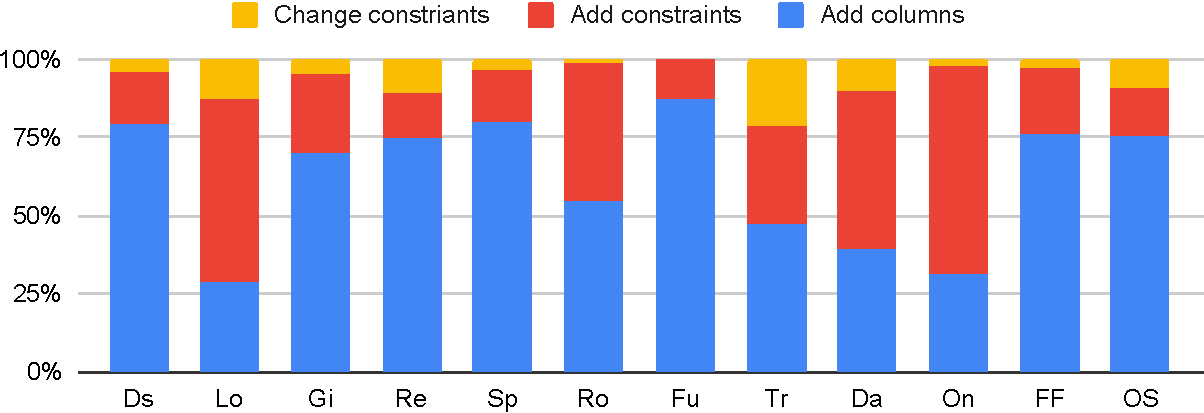
\includegraphics[width=0.6\columnwidth]{constraints//figs/breakdown-release.pdf}
    \caption{Breakdown of \# of adding/changing constraints 
\\   
%\junwen{the figure of release unit is saved as figs/breakdown-release.pdf}
}

    \label{fig:constraints-num}
\end{figure}


\paragraph{\bf Summary} It is problematic
that around or more than a quarter of constraint-related code changes in
most applications are about adding constraints to already existing data columns. This indicates a widely existing vulnerability that allows constraint-violating data to be stored into the database before the correct constraints are imposed. 
Tools are needed to help developers add 
suitable constraints whenever a new data column is created and 
warn of data that is incompatible with the newly added constraints.
  

% \begin{figure}[h]
%     \centering
%     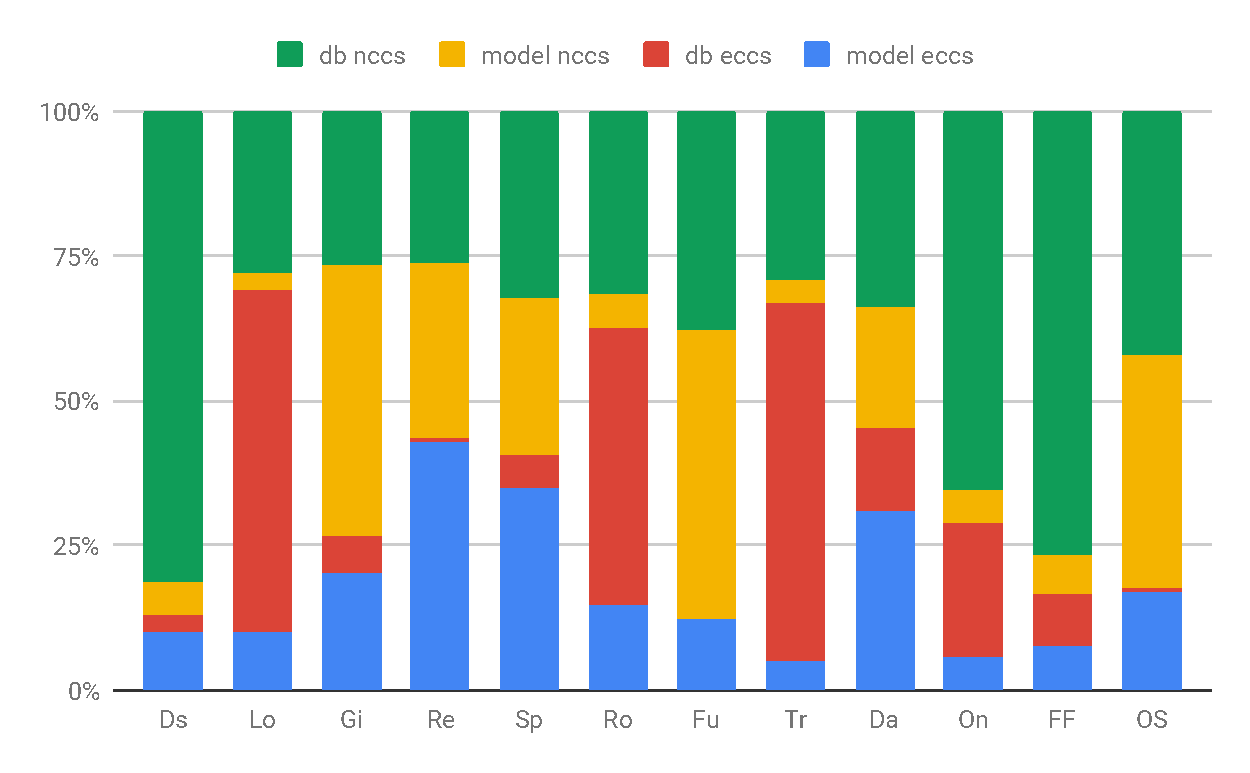
\includegraphics[width=\columnwidth]{figs/existing-new-columns.pdf}
%     \caption{Breakdown of \# of constraints on new/exsiting columns}
%     \footnotesize{nccs: adding constraints on new columns; 
%     eccs: 
%     adding constraints on existing columns}
%     \label{fig:exist-column}
% \end{figure}


% Later
% \begin{figure}[h]
%     \centering
%     \includegraphics[width=\columnwidth]{figs/total.pdf}
%     \caption{Trend of Changing/adding constraints towards line of code change\shan{???first, may want to draw the figures in a different way; second, if absolutely no trend, not worth the space}}
%     \label{fig:exist-column}
% \end{figure}

\section{Constraint-related issues}
\label{sec:causes}
% After studying the \numissues data constraint issues reported in the applications' bug-tracking systems, 
 We categorize \numissues real-world issues 
 into 4 types as shown in Table \ref{tab:issuecat}.
 
 \iffalse 
 :
 (1) data constraints located at different software components conflict with
 each other (WHERE issue); (2) the exact requirement imposed by a data constraint
 conflicts with what the users or the application logic actually expects 
 (WHAT issue); (3) data constraints specified in different code versions conflict
 with each other (WHEN issue); and (4) a constraint's violation-checking result
 is not properly delivered to web users (HOW issue).
 \fi 



\subsection{WHERE is the constraint specified?}
\label{subsec:where}
As discussed, application and DB constraints for the same data field can be inconsistent with each other. Such inconsistencies contributed to 24 out of the 114 issues.

\paragraph{\bf Application constraints looser than DB constraints} 13 out of 24 issues fall into this category. In 12 of them, the constraint is completely missing in application layer while the rest one issue happens because the length constraint has a smaller value in database layer than in application layer.
In these cases, a record saving operation would pass the application server's
checking but fail in the DB, causing a web page crash
with an unhandled raw DB error thrown to end users, which is
often difficult to understand and causes poor user experience. The example discussed in 
Figure \ref{fig:crossstack} is an illustration. 

\paragraph{\bf Application constraints stricter than DB constraints} 11 out of 24 issues fall into this category. In 9 of them, application constraints are not defined in database layer at all while the rest two are caused by that length constraint has smaller value in application layer than in database layer.  
In these cases, the application misbehaves as the administrator/user
directly 
%\shan{who exactly can issue SQL request to DB server directly?}
changes database records through SQL queries in a way that violates application constraints. This happens quite often.   For example, Spree \cite{spree}, an on-line shopping system, has 4 issues caused by administrators modifying database content through direct SQL requests. Discourse \cite{discourse} even has scripts that bypass model constraints to import other forum applications' data. 

Figure~\ref{fig:spree-3829-different} shows such an issue~\cite{spree-3829} in Spree. As shown in (b), each {\tt LineItem} is associated with a {\tt variant} object and a {\tt presence} constraint is used to ensure the existence of every associated {\tt variant}. This ensures that an expression like
{\tt item.variant.image} in (a) is never null.
%Specifically, this presence constraint is checked whenever an {\tt LineItem} object is saved by the application, and it would cause the saving to fail if the associated {\tt variant} object does not exist. 
However, this constraint does not exist in the database. In this bug report,
an adminstrator accidentally deleted a {\tt variant} record in the DB
that is associated with a {\tt LineItem} record, and that
led to a null pointer error when he tried to display 
an order through the code in Figure~\ref{fig:spree-3829-different}a. 
%In the spree issue, only admin users will be affected by the corrupted data. However, there are other issues such as Discourse-30278 in which normal users suffer from null-pointer errors with page crashes because one post's topic has been deleted. 

\begin{table}[]
\centering
\caption{Data-constraint issues in real-world apps}
\label{tab:issuecat}
\setlength{\tabcolsep}{4pt}  
\resizebox{0.6\columnwidth}{!}{
% \begin{tabular}{lrrrrrr}
% \toprule 
% & WHERE
% &  \multicolumn{2}{c}{WHAT}   & WHEN  & HOW & SUM  \\ 
% \cmidrule{3-4}
% & 
% &  vs. code  & vs. user  &   &  &   \\ 
% \midrule
% Ds  & 3  & 0  & 6  & 2  & 2  & 13  \\ \midrule
% Lo  & 0  & 1  & 0  & 0  & 0  & 1   \\ \midrule
% Gi  & 3  & 8  & 0  & 4  & 1  & 16  \\ \midrule
% Re  & 7  & 11 & 4  & 1  & 7  & 30  \\ \midrule
% Sp  & 8  & 14 & 3  & 3  & 3  & 31  \\ \midrule
% Ro  & 0  & 1  & 1  & 0  & 0  & 2   \\ \midrule
% Fu  & 1  & 0  & 0  & 0  & 0  & 1   \\ \midrule
% Tr  & 0  & 0  & 1  & 1  & 0  & 2   \\ \midrule
% Da  & 0  & 4  & 1  & 1  & 5  & 11  \\ \midrule
% On  & 2  & 2  & 1  & 0  & 0  & 5   \\ \midrule
% FF  & 0  & 0  & 0  & 0  & 0  & 0   \\ \midrule
% OSM & 0  & 0  & 0  & 0  & 2  & 2   \\ \midrule
% SUM & 24 & 41 & 17 & 12 & 20 & 114 \\ \bottomrule
% \end{tabular}

\begin{tabular}{@{}rrrrrrrrrrrrrrr@{}}
\toprule
                      &          & Ds & Lo & Gi & Re & Sp & Ro & Fu & Tr & Da & On & FF & OSM & SUM \\ \midrule
WHERE                 &          & 3  & 0  & 3  & 7  & 8  & 0  & 1  & 0  & 0  & 2  & 0  & 0   & 24  \\ \midrule
\multirow{2}{*}{WHAT} & vs. code & 0  & 1  & 8  & 11 & 14 & 1  & 0  & 0  & 4  & 2  & 0  & 0   & 41  \\ \cmidrule(l){2-15} 
                      & vs. user & 6  & 0  & 0  & 4  & 3  & 1  & 0  & 1  & 1  & 1  & 0  & 0   & 17  \\ \midrule
WHEN                  &          & 3  & 0  & 4  & 1  & 3  & 0  & 0  & 0  & 1  & 0  & 0  & 0   & 12  \\ \midrule
HOW                   &          & 2  & 0  & 1  & 7  & 3  & 0  & 0  & 0  & 5  & 0  & 0  & 2   & 20  \\ \midrule
SUM                   &          & 14 & 1  & 16 & 30 & 31 & 2  & 1  & 1  & 11 & 5  & 0  & 2   & 114 \\ 


\bottomrule
\end{tabular}
}
\footnotesize{}
\end{table}


\begin{figure}
    \centering
    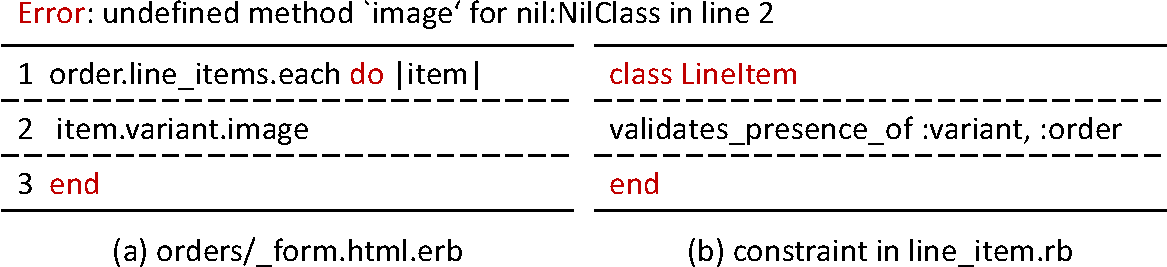
\includegraphics[width=0.6\columnwidth]{constraints/figs/spree-3829-different2.pdf}
    
    \caption{Constraint mismatch in Spree}
    
    \label{fig:spree-3829-different}
\end{figure}

% The could also be incompatibility between html layer and model 

% \junwen{We don't have issues caused by inconsistency of html constraint and model constraint. If there is, the symptom would be  misleading error message. }
% \shan{I remember you started looking into html-end constraint because you saw some
% inconsistency. right?}

\paragraph{\bf Summary}
As shown by real-world issues, inconsistencies between application 
 and database constraints cause problems, including
web page crashes and poor user experience.
Considering the hundreds and thousands of constraints that exist in the DB
but not in application and vice versa 
(see Section~\ref{sec:one_where}), 
this problem could be much more severe and widespread than
what reflected by the issue reports.
Automatically detecting such constraint inconsistencies will be very helpful, which we further explore in Section \ref{sec:solution}.

\subsection{WHAT is the constraint about?}
\label{subsec:what}
The most common problem is a mismatch between how data is supposed to be used in the application and the constraints imposed on it. This accounts for 
58 out of \numissues issues. 
%\alvin{i don't quite get what you mean. you mean conflict between constraints specified in app vs constraints specified in the db?}\shan{no, it is like the constraint said this should be an integer, but the application tries to get the square root of this data, which indicates the constraint should positive-integer, not just integer.}


\subsubsection{{Conflict with user needs}}

Users sometimes would relax an existing constraint,
such as increasing the input length of name field in tracker from 30 to 100 (Redmine-23235 \cite{redmine-25235}).
These contribute to about 10\% of the issues in our study.
%Another user in Tracks asks ``The passwords are limited to 40 characters.
%I don't like the limit, so is it possible to increase it?''. 
%The solution is simple as shown in Figure~\ref{fig:tracks-1921-passwordlength}, 
%in Discourse-79684: ``On our site users sometimes want really long `About Me' descriptions in their profiles but it is by default limited to 3000 characters. Is there any easy way to bump this up?''.
%Similarly, a user posted an issue in Discourse \cite{discourse.75453}, saying ``Does anyone know if there is a way to modify the maximum character limit for category names? I need to ...".
%put an English title, followed by the French equivalent, but I am running out of room to do both.''. 
Developers usually satisfy the users' desires and change constraints
accordingly. 

\iffalse
In Redmine, the corresponding length-constraint was only
specified in application, not in DB, and the patch simply changed
the application validation function parameter to allow longer
inputs; in Discourse, since Category-name has its length constraint
specified in both application and in DB, the patch changed
both places.
\fi 

% Sometimes, the constraints validation needs to be skipped. For example, in Spree-7389, user says ``There is validation for Address model for zipcode. It's always check it even though this may be problem because for example Hong Kong doesn't have zipcodes.''

\iffalse 
\begin{figure}
    \centering
    \includegraphics[width=0.8\columnwidth]{figs/tracks-1921-passwordlength.pdf}
    \caption{Too tight constraint in Tracks}
    \label{fig:tracks-1921-passwordlength}
    %link: https://github.com/TracksApp/tracks/issues/1921
\end{figure}
\fi 

\paragraph{\bf Summary}  For certain type of constraints, like the
length constraint, it is difficult to have one setting that satisfies all users' needs. It would be helpful if refactoring routines can be designed to turn a fixed-setting constraint into configurable. %\shan{1.none of your example above is about configurable; 2.it is better to suggest some automation, like suggesting refactoring that makes some constraints that involve numerical bounds to be user configurable.}. 


\subsubsection{{Conflict with application needs}}
\label{sec:what_app}
Many constraints are created to guarantee program invariants
that are crucial to applications' functional correctness. 
Constraints that are insufficient or even conflicting with how the corresponding
data is used by the application contribute to more than one third of all the issues
in our study.

\paragraph{\textbf{Type conflicts}}
These constraints treat a data field as having a general type, but
the application uses the data field in a more specialized way
that demands tighter constraints. In one Redmine issue~\cite{redmine-9394}, a user noticed that she can input  invalid dates like
``2011-10-33'' without triggering any errors. 
This problem happened because Redmine only used a regular expression ``\textbackslash d\{4\}-\textbackslash d\{2\}-\textbackslash d\{2\}\textdollar'' to make sure the input follows the ``yyyy-mm-dd'' format without more detailed checking.
To solve this problem, Redmine later added ``value.to\_date'' to check whether the input   can really be converted to a date or not in the custom validate function shown in Figure~\ref{fig:redmine-9394-tooloose}.  

\begin{figure}
    \centering
    \includegraphics[width=0.6\columnwidth]{constraints/figs/redmine-9394-tooloose.pdf}
    \vspace{-0.2in}
    \caption{Type conflict example in Redmine}
    %\vspace{-0.1in}
    \label{fig:redmine-9394-tooloose}
\end{figure}

\textbf{Case sensitivity conflicts.} 
{\it Uniqueness} is a common constraint associated with a data field to
avoid duplication, like preventing two users from having the same ID. 
A common problem is that a field is written to the DB in
a case-sensitive way of uniqueness, while used or searched in a
case-insensitive way, or vice versa. Such inconsistency can lead to severe software misbehavior. 

In a Gitlab issue~\cite{gitlab-24493}, a user's profile email is all in lower case, but she committed code with an upper-case letter in her email, which then cannot
be matched to her profile. What is annoying was that she was 
unable to add the different casing as an alias, as Gitlab said
the email was ``already in use.''  This happens because when a user-email is stored into DB, the uniqueness checking
is case insensitive---``abc@example.com'' is treated the same as ``ABC@example.com.'' However, when the application searches for code commit using email
as the index, the search is case sensitive --- code committed by
``ABC@example.com'' cannot be retrieved by a search using
``abc@example.com.'' The patch made the search also
case insensitive, thus always converting the input email to pure-lowercase before the
search, as shown in Figure~\ref{fig:gitlabcasesensitive}. 

\begin{figure}
    \centering
    \includegraphics[width=0.6\columnwidth]{constraints/figs/gitlab-issue.pdf}
    \caption{Case sensitivity conflict example in Gitlab}
    %\vspace{-0.1in}
    \label{fig:gitlabcasesensitive}
\end{figure}

\textbf{Boundary value conflicts.} There are cases where certain
values of a data field are allowed by the application logic, 
but disallowed by the constraints. For example, in the typical checkout flow of Spree, users would enter their delivery details, then proceed to a payments page to enter discounts and payment details, and then finally arrive at a confirmation page. However, in one Spree issue\cite{spree-6673}, a user complained that when she entered a discount coupon that reduced the price to zero---which was actually a valid use case---the application did not allow him to proceed, and instead redirected back to the delivery page. The source of the bug was a constraint in the model layer ({\tt models/spree/order.rb}) which
%, in order to proceed to the next stage of the checkout flow, 
incorrectly required the value of the {\tt total} field to be strictly greater than zero.

\iffalse 
\begin{figure}
    \centering
    \includegraphics[width=\columnwidth]{figs/spree-issue.pdf}
    %\vspace{-0.1in}
    \caption{Boundary value inconsistency in Spree}
    \label{fig:spreerwinconsistency}
\end{figure}
\fi 

\paragraph{\bf Summary}
Failure symptoms of these bugs are quite different from all the other types 
of bugs (WHERE, WHEN, HOW). They can lead to severe software misbehavior or even
disable an entire feature of a web application.  
It would be ideal if a program analysis tool can compare how a data field
is used in software and identify inconsistency between how it is used and 
how it is constrained. This is challenging for generic data
types and data usage, but is feasible for specific types of 
problems, which we explore
in Sec. \ref{sec:solution}.


\subsection{WHEN is the constraint created?}
\label{subsec:when}

When upgrading an application, sometimes newly added or changed constraints might be incompatible with old data. 
12 issues are caused by such inconsistency across versions. 
The failure symptoms vary based on the different program context where the 
tighter constraint is checked.

\paragraph{\textbf{Read path}}
When a constraint is newly created or tightened along a DB-record loading code
path (e.g., front-end
constraint or application sanity-check changes), an  
incompatible new constraint can cause failures in
loading old data and hence severe functionality problems.
The Diaspora example in Section~\ref{sec:intro} belongs to this
category: the password's length requirement tightened and hence invalidated many old passwords.

\iffalse 
In the old version of Diaspora, it is allowed to set the password with length smaller than three. In one commit, developers have added an constraint in HTML level with format ``......+'' which limits the password  to be equal or longer than 6 characters. This causes many users, whose
passwords are shorter than 6 character, to fail to login to Diaspora with the 
unhelpful error-information saying ``Please use the required format''. 
Their solution is to remove the newly added constraints on the password length.


\begin{figure}
    \centering
    \includegraphics[width=\columnwidth]{figs/diaspora-4221-password.pdf}
    \vspace{-0.2in}
    \caption{Old data conflicts with new constraints (Diaspora)}
    \label{fig:diaspora-4221-password}
\end{figure}
\fi 

\paragraph{\textbf{Write path}}
When a constraint is newly created or tightened along a path that intends to
save a record to the database (e.g., all the application-validation constraints
and database constraints), the incompatibility between the new constraint
and old data can be triggered under the following two circumstances.
 

First, all the old data in the database will be checked against the new set 
of DB constraints during a migration process during
application upgrade. 
Inconsistency between old data and new DB constraints can cause an upgrade failure.
For example,
one Gitlab issue~\cite{gitlab-36919} complains that they failed to upgrade from version 9.4.5 to 9.5.0 due to {\tt NotNullViolation} during data migration. As shown in Figure~\ref{fig:gitlab-36919-when}, the {\tt decription\_html} column was added 
to Gitlab before version 9.4.5 (in the ``20160829...'' migration file) and was filled with {\tt null}s by 
default.\footnote{When no default value is specified in {\tt add\_column}, {\tt null} is used as the default value.}
% in migration add\_markdown\_cache\_columns.rb before 9.4.5, but the column still has null value
Later on, in the ``20170809...'' migration (shown in the Figure~\ref{fig:gitlab-36919-when}), a non-null constraint 
was added to the column through the API {\tt change\_column\_null} with parameter {\tt false}. This caused 
many users' upgrade to fail because there were many old records with
a default {\tt null} in that column. 
%There are two solutions to solve this issue, one is to change the constraint, 
The patch removed the ``non null'' constraint to the {\tt description\_html} column, as shown in 
Figure~\ref{fig:gitlab-36919-when}. 
%Of course, an alternative solution is to set a not-null default value for the column as shown in Figure~\ref{fig:gitlab-36919-when}.
%--edit to here
%We have also seen cases where the migration file added a new column with a {\tt not-null} constraint without setting default value for it. As a result, the system by default fills the new column with {\tt null} and immediately leads to migration/software-upgrade errors such as that in Gitlab-46862. 


Second, even if all the old data is validated against DB constraints and the application has successfully upgraded, the old data might still conflict
with new constraints specified through the application validation APIs that did not exist in the prior version.
This can lead to problems when the application allows users to edit an existing
 record---users may have trouble in saving an edited record back.
In one Discourse issue~\cite{discourse-89148}, a user complained that she made a small edit to an old post's  title, but was unable to save with an error message stating that the title was invalid.
It turned out that, the 
title's length constraint has been changed from 30
 to 20 characters in the application's validation function. That old post's title contained
28 characters; the small edit did not change the title length. So, the old post can still be loaded by the application, but cannot be saved back after such small edits.
 

 

\begin{figure}
    \centering
    \includegraphics[width=0.6\columnwidth]{constraints/figs/gitlab-36919-when.pdf}
    \caption{Old data conflicts with new constraints in Gitlab}
    %\vspace{-0.1in}
    \label{fig:gitlab-36919-when}
\end{figure}

\paragraph{\bf Summary}  Given the frequent constraint addition and changing
in web applications, it is inevitable that old data may
become incompatible with new constraints. It would be helpful if automated 
tools can provide warnings for developers when constraints become
tighter in a new version, particularly (1) if the migration file has high probability to
fail (e.g., specifying a constraint that conflicts with a column's default value), then developers should fix the migration
file; (2) if the application allows editing old data, then developers should probably 
add explicit warning to users about the risk of editing old data; and finally
(3) the case of having tighter constraints that limit the reading of old data should be avoided. We explore this in Section~\ref{sec:solution}.

\subsection{HOW are the checking results delivered?}
%\utsav{Possibly include results on what portion of custom validations might be missing errors}
\label{subsec:how}

Constraint violation is common in web applications, as web users cannot anticipate all the constraints
in advance and will inevitably input constraint-violating data. Consequently,
delivering informative and friendly error messages is crucial to web applications'
user experience. 20 issues in our study are about this problem. 
 
These 20 issues are mostly related to application-validation constraints.
Rails validation APIs provide default error messages that are mostly 
clear.\footnote{Section~\ref{sec:solution} discusses cases when the default message is unclear
and how we enhance it.} However, developers 
sometimes forgot to display the error message associated with the validation
APIs (8 cases) and sometimes override the default message with
uninformative generic messages (12 cases), which led to user complaints.
For example,
in a Diaspora issue~\cite{diaspora-5090}, a user complained that when he tried to post a long article, the posting failed with an unhelpful error message ``Failed to post!'' 
%The user demanded ``a more descriptive error message''. 
Developers found out that their code in {\tt posts\_controller} forgot to render the error message
defined in {\tt post}'s validation function. The patch fixed this problem
and would display the required length limit,
as shown in Figure~\ref{fig:diaspora-5151-errormsg}.
%\shan{Junwen, please make the patch figure simpler, only
%reflecting the change to show the length limit.}
%by ``please make your post less than 65536 characters''. Although this is not the default error message provided by Rails, the information revealed is the same. 
%In this particularly case, users later further requested to know not only the post limit but also the length of their failed submission, which was satisfied by later patches. 
%So eventually the error message was changed to ``Please make your post fewer than 65536 characters. Right now it is \%\{length\} characters'', in which  \%\{length\} is the current length of users' input post.
\begin{figure}
    \centering
    \includegraphics[width=0.6\columnwidth]{constraints/figs/diaspora-5990-errormsg-cp.pdf}
    \caption{Unclear error message in Diaspora}
    \label{fig:diaspora-5151-errormsg}
    %link: https://github.com/diaspora/diaspora/issues/2481
\end{figure}

\paragraph{\bf Summary} Developers should be reminded to display error messages associated with validation APIs. Future IDEs should automatically 
synthesize default error checking and error-message display code. 
Improving the quality of default and custom error message is crucial to
user experience. We will explore this in Section~\ref{sec:solution}.
%Some issues however requires a better understanding of the application behavior facing errors.
 

% \iffalse
% In Diaspora-2481, many users complain that they tried many times to reset password but failed with a bunch of error messages as shown in Figure~\ref{fig:diaspora-2481-unclear}~(b), which is very confusing since in the password reset page, there are only two fields for the new password and confirmation of it. There is no email and username on that page at all, not to mention the error message. The developer figured out this happens because the email address has been invited to Diaspora, but hasn't accepted the invitation yet, which is not reflected through the error message at all. And do not underestimate the importance of the error message. They are crucial to the popularity of the applications. A user says ``I had no idea what those messages meant, and a normal user would simply abandon their account.''. \shan{yeah, this
% bug is interesting. However, are we doing anything to help resolve this problem?
% the problem here seems to be that the error message is complaining about a field
% that the user entered in a previous page, right? That seems to be different
% from the problem you guys worked on?}

% \begin{figure}
%     \centering
%     \includegraphics[width=\columnwidth]{figs/diaspora-2481-unclear.pdf}
%     \caption{Unclear error message in Diaspora}
%     \label{fig:diaspora-2481-unclear}
%     %link: https://github.com/diaspora/diaspora/issues/2481
% \end{figure}

% \endif

 \section{Solutions \& Evaluation}
\label{sec:solution}
  
%Guided by the patterns discussed above, we explore detecting some of these problems  in the {\bf latest} versions of these 12 applications. 

We now discuss our experience in building tools to automatically discover the anti-patterns discussed earlier. We focus on applying them to the latest versions of the studied applications, as these represent potential bugs that have not been discovered.

\subsection{Where issues}

As discussed in Section~\ref{sec:one_where}, our scripts can automatically find more than 1000 string-length DB constraints that are missing in application, and more than 400 application built-in-validation constraints
 that are missing in the DB. We reported 16 of them covering different types, with 12 of them already confirmed by developers from 3 applications (Lo, Ds, FF).

In addition, we extended our scripts to automatically find conflicting cases, where
the same type of constraint, like length, is specified for the same 
data field in both database and application, but the exact constraint requirement is different.

As shown in Table~\ref{table:mismatchdbmodel}, our checker reported 138 conflicting constraints in total.
Our manual checking confirmed that 133 of them are true conflicts and 5 are false positives.

These 133 conflicts include 84 cases where
applications' length constraints are tighter than the DB's, 4 cases in the other way, 1 case where the columns referenced by uniqueness constraints did not exactly match, and 44 cases where the range or type of numeric values allowed in DB did not match the corresponding restriction in the model. 
For example, our results showed that, in the Tracks application, there was a string field {\tt description} in model {\tt Todo} for which the length in DB was limited to 255 characters, but was limited to 300 in the model. 
%This would cause requests to fail if a user entered a description between these two lengths. 
We reported this mismatch to developers and received confirmation that it was indeed a bug. 
As another example, we found 5 instances in OpenStreetMap where developers meant to require 
fields to be integers in both the DB and application. However, developers had typos in their use of validation APIs, which caused the application-level numericality constraints to be silently ignored. 
We reported this to developers, who then fixed the bug.

% \begin{table} 
\setlength{\tabcolsep}{3pt}  
\caption{\# Reported Issues}
\resizebox{\columnwidth}{!}{
\begin{tabular}{lrrrrrrrrrrrr}

\toprule
& Ds   & Lo  & Gi   & Re  & Sp  & Ro  & Fu & Tr  & Da  & On  & FF  & OS  \\
\midrule
Reported & 5 & 6 & 0 & 1 & 0 & 0 & 0 & 1 & 1 & 0 & 3 & 20 \\
\midrule
Confirmed & 2 & 6 & 0 & 0 & 0 & 0 & 0 & 1 & 1 & 0 & 3 & 20 \\ 
% data source https://docs.google.com/spreadsheets/d/1d9wh0BxLLgQaSKSxFTA3ou5RH7P5D8LKaHQ1paU45u8/edit?usp=sharing
\bottomrule
\end{tabular}
}
\label{table:reportedissues}
\end{table}

% Table~\ref{table:reportedissues} shows the detailed number of our reported and confirmed issues. 


%\shan{do you have any good value range example?}\utsav{Pretty much any time a developer specifies a range in model, this results in mismatch, because no explicitly-defined ranges exist in DB layer (i.e. it is always implicit [INT\_MIN, INT\_MAX]). Example follows but we do not report anything because we have no clear solution.} 
As an example of range mismatch, there was a case in Spree where the field {\tt price} must be greater than or equal to zero. However, in the DB, the field type was {\tt decimal} which allows negative values.

Among the 5 false positives, 3 were caused by our tool's limited ability in handling non-literal expressions, and the others were related to our tool's inability to distinguish between array length and string length validations.

\begin{table} 
\centering
\setlength{\tabcolsep}{3pt}  
\caption{\# Mismatch constraints between DB-Model}
\resizebox{0.7\columnwidth}{!}{
\begin{tabular}{lrrrrrrrrrrrr}

\toprule
& Ds   & Lo  & Gi   & Re  & Sp  & Ro  & Fu & Tr  & Da  & On  & FF  & OS  \\
\midrule
Length - DB looser & 5 & 7 & 12 & 9 & 0 & 25 & 0 & 4 & 4 & 11 & 0 & 7\\
\midrule
Length - DB tighter  & 0 & 0 & 0 & 0 & 0 & 3 & 0 & 1 & 0 & 0 & 0 & 0 \\
\midrule
Uniqueness  & 1 & 0 & 0 & 0 & 0 & 0 & 0 & 0 & 0 & 0 & 0 & 0 \\
\midrule
Numericality  & 4 & 0 & 24 & 1 & 6 & 0 & 3 & 0 & 0 & 0 & 3 & 3 \\
\midrule
{\it False positives}  & 0 & 0 & 2 & 3 & 0 & 0 & 0 & 0 & 0 & 0 & 0 & 0 \\
\midrule
Total  & 10 & 7 & 38 & 13 & 6 & 28 & 3 & 5 & 4 & 11 & 3 & 10 \\
% \midrule
% Reported & 5 & 6 & 0 & 1 & 0 & 0 & 0 & 1 & 1 & 0 & 3 & 20 \\
% \midrule
% Confirmed & 2 & 6 & 0 & 0 & 0 & 0 & 0 & 1 & 1 & 0 & 3 & 20 \\ 

% data source https://docs.google.com/spreadsheets/d/1d9wh0BxLLgQaSKSxFTA3ou5RH7P5D8LKaHQ1paU45u8/edit?usp=sharing
\bottomrule
\end{tabular}
\vspace{-0.3in}
}
\label{table:mismatchdbmodel}
\end{table}


\subsection{What issues}
We built a checker to detect ``case-sensitivity conflicts'' discussed
in Section~\ref{sec:what_app}. Our checker first identifies every field that has case insensitive constraints specified by the validation API {\tt validates\_ uniqueness\_of:field} and {\tt case\_sensitive:false}, then checks all the statements that issue a read query to load such a field to see if the loading is ever done in a case sensitive way. To identify all those read queries, we
used an existing static analysis framework for Rails~\cite{yang:fse18:powerstation}; to identify case-sensitive loading, we check whether the query is directly ordered by the field 
({\tt .order(`field')}) or filtered on the field ({\tt .where(field: params)}) 
without case conversion. 

Our checker found 19 issues in latest versions --- 14 in Lobsters, 3 in Redmine, 2 in Tracks. Our manual checking confirmed these are all bugs (no false positives). We also got confirmation
from developers of Lobsters and Redmine. Redmine has already added our patch to their next major release 4.1.0. 


\subsection{When issues}

Given two code versions, to detect inconsistency between old data and new constraints, we extend our script that examines constraint changes across versions (Section~\ref{sec:evolve}) to see if new constraints are added or existing
constraints are tightened. We then further check whether the application allows editing existing
DB data, whether the default value conflicts with the new/changed constraint, and whether the migration
file updates the corresponding column in the database, which is a common way to avoid incompatibility
problems. Due to space constraints, we omit details of the algorithm.
%by checking the properties of the constraint for example whether the inclusion array of an inclusion constraint has shrunken\shan{how do you know it is tightened or not? Do you only reason about tightening
%for specific type of constraints?}. 
%If there is a new/tightened application built-in validation constraint, our checker further checks if the 
%related object can be edited in the application by checking whether there is an edit action that will update or save the object \shan{how do you know it is edited?} --- if it can,
%this is a potential problem;
%if there is a new/tightened DB constraint, our checker checks if the default value of that data field, 
%which is specified in migration files and assumed to satisfy the new/tightened constraint\shan{do you need some
%kind of symbolic reasoning to know this?} --- if it does not, this is a potential problem. 
%In both cases, our checker also checks the migration files to see if there are statements there that 
%convert old data to match the new constraints\shan{how exactly is that checking done?}\junwen{To avoid false positive, what I have done here is to check whether the migration file has any statement to update the field or set the default value, if there is, I will consider it's used to meet the new/tightened constraints}. If there is a new/tightened html validation constraint, we check whether they are generated from the login form of the application, if so, they might prevent users from logging. 

We applied our checker to the problematic upgrade pointed out by the 12 known issues in our study
(Section~\ref{subsec:when}), and confirmed that it can detect all these 12 issues with no false positives. It did not find problems with the latest upgrade 
%\shan{two commits? two releases?} \junwen{for app with release, it's release, for app without release, it's the latest commit and (latest - 100)th commit}
of these applications.  
%TODO for future: apply to every commit 

\subsection{How issues}
\label{sec:how}
%To understand how the error message is delivered generally, we have collected the statistics about default/customized error messages of built-in validation API, and also whether error message is created for customized validation API and non-API sanity checking. 

\paragraph{\bf Improving built-in error messages.} 
Rails built-in validation APIs provide default error messages that are used
by developers in most cases, only overridden
in 2\% of the cases across all studied applications. Consequently,
having informative default messages is crucial.

\begin{table} 
\centering
\setlength{\tabcolsep}{2pt}  
\caption{Our enhancement to default error messages}
\resizebox{0.7\columnwidth}{!}{
\begin{tabular}{lll}
\toprule
& Default & Enhanced\\
\midrule 
{\tt inclusion\_of} &``invalid''& ``have to take values from \{A, B, ...\}''\\
\midrule
{\tt exclusion\_of} &``reserved''& ``cannot take values from \{A, B, ...\}''\\
\midrule 
{\tt confirmation\_of}& ``invalid''&``Case does not match with earlier input''\\
\midrule
{\tt uniqueness\_of}&``invalid''&``Not unique in case (in)sensitive comparison''\\
\midrule 
{\tt associated}&``o is invalid''& ``field f of object o is invalid''\\
\bottomrule
\end{tabular}
%\vspace{-0.1in}
}
\label{table:msgenhance}
\end{table}

\begin{table}[]
\centering
\caption{User study results}
\footnotesize{
\setlength{\tabcolsep}{2pt}  
%\resizebox{\columnwidth}{!}{
\begin{tabular}{lrrr}
\toprule 
% & \multicolumn{3}{c}{Form input - average \# of input attempts} \\
%\cmidrule{2-4}
Task-1    & \# input attempts w/ modified & \# attempts w/ default & Decrease \\
\midrule
Inclusion & 2.2 & 3.1 & 30\% \\ \midrule
Associated & 2.3 & 3.4 & 33\% \\
\midrule
\midrule
%& \multicolumn{3}{c}{User preference}  \\
%\cmidrule{2-4}
Task-2 & \% of users prefer modified &  \% prefer default & No preference\\ 
\midrule
Exclusion  & 74\%  & 22\% & 4\%  \\ \midrule
Confirmation  & 81\%  & 8\%  & 11\%  \\ \midrule
Uniqueness  & 74\%  & 16\%  & 10\%  \\
\bottomrule
\end{tabular}
%\vspace{-0.1in}
%}
}
\label{table:studyresults}
\footnotesize{}
\end{table}


We found that 5 APIs' default messages can be more informative, as shown in Table~\ref{table:msgenhance}. 
For example, {\tt validates\_confirmation\_of} ensures that a
field and its confirmation field have the same content. Instead of only saying the input is ``invalid,''
%{\tt validates\_uniqueness\_of} repo whether an input value is unique. 
%In practice, the violation is often caused by case sensitivity.
we add information on whether the matching failure is caused by case sensitivity, 
so the user can decide whether to change just the case or the actual value.
As another example, {\tt validates\_associated} checks if every field of a sub-object $o$, which is associated with another object, is valid (e.g., a ``photo'' is a nested object of ``profile'', and has
fields ``source\_url'', ``width'', ``height'').
%\shan{what is a sub-object? Can you give a concrete but brief example?}\junwen{say an account is associated with a user, user is the object with validates\_associated: account, account is the subobject, when saving the user, it will tell you `account is invalid', will not tell you the detailed reason why account is invalid as described in the StackOverflow post
If the validation of any field of $o$ fails, the default message states only that the entire 
$o$ is invalid. 
Our enhancement lets the user know which specific field (e.g., ``source\_url'' or ``width'' or ``height'') is incorrect and how to revise.

%\shan{shan: Please provide more details about why they are not informa-tive and what exact enhancement you did} 

We have implemented a library (i.e., a Ruby gem) to overwrite the Rails default error message with our advanced ones. Our gem redefined the existing error message generation functions with custom ones that incorporated more information. 

\paragraph{User Study} To evaluate our error-message changes, we recruited 100 participants using Amazon Mechanical Turk (MTurk). The participants are all live in US and are at least 18 years old with higher than 95\% MTurk Task Approval rate.
We asked users to perform two tasks. First, users provided answers to questions such as, enter a title, first name, and last name; or try and enter a unique value for a given category. If they fail to provide a valid answer, we either provide them with the Rails default error message, or our improved error message. In each case, we track the number of retries required for the user to reach a valid input, and if they cannot after 5 retries, we skip to the next question. Each user was given 2 of these tasks.
In the second task, we provide a webpage screenshot of a question and an incorrect answer-input to that question. The questions are based on the applications we studied. We then show two options for error messages: the default message and the improved  message. We ask the user to rate which error message would be more helpful in arriving at a valid input. Each user was given 3 of these tasks.

 As shown in Table~\ref{table:latestconstraintnum},  
for the first task, our enhanced error messages reduced the number of tries users took to reach valid inputs by about 30\%;
for the second task, we find 74--81\% of users preferred our enhanced error messages, depending on the type of validation.



\paragraph{\bf Detecting missed error messages.} Developers are required to provide error messages for 
custom validations through the API {\tt object.errors.add(msg)}. We extend our script that identifies custom validation functions to further check
if an error message is provided.
We found one case in Diaspora where the error message is missing. This is actually a severe problem:
since Rails uses the count of error messages to determine the validity of an object, an invalid object
can then be incorrectly treated as valid and lead to application failures. 
We reported this bug to Diaspora developers, who have confirmed that this is indeed a bug.
%\shan{Can you guys report this case to the developers? sound severe?}

\paragraph{\bf Detecting missed error rendering.}
%It is also possible that developers may simply forget to display already specified error messages. 
Since there are many ways to render error messages on a web page, it is difficult to automatically
detect this problem.
We randomly chose 45 HTML pages with forms across 12 applications, and manually checked if error messages caused by invalid inputs were rendered.
We found one case where the message would never be rendered: 
%One case is related to a URL-type field, 
on a page in OpenStreetMap that asks users to input a URL,
%register OAuth clients. 
when the input has an improper format, the web page
marks the field with red color, without rendering the error message associated with the
constraint. 
%Another case turns out to be a false positive: although the error message associated with length validation is never rendered, there is a front-end HTML constraint that conducts the same validation and does render an error message when there is a violation.

%%%%%%%%%%%%%%%%COMMENT OUT%%%%%%%%%%%%%%
\iffalse 
\begin{table}[h]
\caption{\# Messages overridden by developer (built-in API)}
\resizebox{\columnwidth}{!}{
\begin{tabular}{lrrrrrrrrrrrr}

\toprule
& Ds   & Lo  & Gi   & Re  & Sp  & Ro  & Fu & Tr  & Da  & On  & FF  & OS  \\
\midrule
total (built-in) & 151 & 31 & 439 & 223 & 118 & 213 & 10 & 26 & 99 & 66 & 14 & 79\\
\midrule
overridden  & 0 & 0 & 17 & 2 & 3 & 1 & 3 & 3 & 0 & 2 & 0 & 0 \\
\bottomrule
\end{tabular}
}
\label{table:builtinerrormsg}
\end{table}
\fi 

\iffalse 
\begin{table}[h]
\caption{\# Messages missing from custom validations}
\resizebox{\columnwidth}{!}{
\begin{tabular}{lrrrrrrrrrrrr}

\toprule
& Ds   & Lo  & Gi   & Re  & Sp  & Ro  & Fu & Tr  & Da  & On  & FF  & OS  \\
\midrule
total (custom) & 18 & 3 & 31 & 28 & 14 & 8 & 0 & 3 & 9 & 17 & 3 & 1\\
\midrule
missing  & 0 & 0 & 0 & 0 & 0 & 0 & 0 & 0 & 1 & 0 & 0 & 0 \\
\bottomrule
\end{tabular}
}
\label{table:customerrormsg}
\end{table}

\fi 
 

\section{Discussion}
\label{sec:threats}
\subsection{Impact of False Positives}
Our scripts for checking constraints inconsistency across layers has some false positives, of which  the vast majority come from two types of constraints: (1) string-length constraints in database, (2) presence constraints in applications. The remaining false positives are due to some validation/migration API call parameters being derived from function calls or non-constant expressions, which we do not currently evaluate. 

Such false positives have limited impact on the paper's findings and are already considered in our finding presentation:

RQ1: This has little impact. The overall trends like many data fields associated with constraints, DB containing most constraints will not be affected by these small number of false positives.

RQ2: This has negligible impact. For instance, the number of versions with constraint changes remains the same even if we do not consider the above two types of constraints;  

RQ3: There is no impact since the real-world issue study is conducted manually;

RQ4: This has negligible impact. All findings in Table 1 still hold, as they either are not related to those two types of constraints or are reported with false positives already pruned or carefully considered. For instance, although our script reported 1,650 database string length constraints missing in the application, we intentionally only highlight ``1000+ string fields ...'', instead of 1,650, in Table 1, exactly because we have taken the potential impact of false positives into account. 

\subsection{Threats to Validity}
 \textbf{Internal Threats to Validity}:
As discussed in 
Section~\ref{sec:back_constraints} and \ref{sec:wherewhat},
we only considered DB constraints declared through Rails built-in migration APIs, but not those through SQL queries, which are extremely rare (fewer than 30
across all 12 applications). 
Our analysis covers only native DB types such as string, numeric, and datetime types, and excludes non-native DB types such as JSON, spatial, or IP format, which together account for less than 1\% of all columns. Front-end constraints specified through JavaScript files were not considered. 
Finally, our static checkers have false positives as discussed in 
Section~\ref{sec:one_where} and \ref{sec:solution}.

\textbf{External Threats to Validity}:
The 12 applications in our study clearly may not represent all real-world applications;
the \numissues issues studied also may not represent all constraint-related issues in these applications;
the 100 participants of our user-study from MTurk may not represent all real-world users. Overall, we have tried our best to conduct an unbiased study.

As discussed in Section~\ref{sec:back_constraints}, other ORM frameworks, like
Django and Hibernate, also let developers specify application and database constraints  like that in Rails.
We sampled 22 constraint-related issue reports from the top 3 popular Django applications on Github, and observed similar
distributions, as shown below. 
\begin{table}[h]
%\caption{Similar issues in Django apps}
\resizebox{\columnwidth}{!}{
\begin{tabular}{@{}lrrrrrr@{}}
\toprule
& WHERE
&  WHAT & WHAT  & WHEN  & HOW & SUM  \\  
& & vs.code & vs.user &  & &\\
\midrule
django-cms \cite{django-cms}& 1     & 2           & 3          & 3    & 1   & 10   \\ \midrule
zulip \cite{zulip}     & 1     & 4           & 2          & 0    & 0   & 7   \\ \midrule
redash \cite{redash}    & 0     & 2           & 0          & 0    & 3   & 5   \\ \bottomrule
\end{tabular}
}
\label{django-issue}
\end{table}






\section{Conclusion}

\label{sec:con}
%DB-backed web applications maintain a huge amount of persistent data. 
Specifying and maintaining
consistent and suitable constraints for data is crucial to ensure the application correctness and usability.
In this paper, we thoroughly studied how data constraints have been specified, maintained, and led to
real-world issues in 12 representative open-source DB-backed applications. Our study shows that
tooling support is needed to help developers manage data constraints, and our checker is the first step towards providing such support.

\chapter{Automated Code Refactoring upon Database-Schema Changes in Web Applications}

\section{Overview}
\label{sec:intro}
Modern web applications often use database engines to 
manage a large amount of user data, such as user profiles in social network applications and transaction
records in on-line shopping platforms~\cite{webapp}.  
The schema of such data goes through changes, such as table renaming, column
deletion, and others, for better performance or functionality when an application evolves \cite{wang2017verifying}.
Unfortunately, it is difficult for developers to keep their code 
consistent with database schema changes all the time, a task we
refer to as \textit{schema-related code refactoring}, with any inconsistency leading
to application crashes.

Schema-related refactoring and
traditional refactoring like class renaming share similarities, given that
popular Object Relational Mapping (ORM) frameworks, such as Rails \cite{rails},  
Django \cite{django}, and Hibernate \cite{hibernate},
allow database data to be
updated and retrieved in an object-oriented way---the name of a database table corresponds to the name of a model class
and the names of table columns are the same as class fields.

%\shan{TODO: we may need to expand the onebody example}
However, they also differ in various aspects, due to the unique nature of persistent data,
as we elaborate below\footnote{Our discussion generally applies to
all web applications developed upon ORM frameworks, although our
examples use Ruby on Rails applications.}.



%Comparing with traditional software, database-backed web applications face the unique code-maintenance challenge of making code changes consistent with database schema changes. Because web applications are often constructed using Object Relational Mapping (ORM) frameworks allowing the properties and relationships of the objects in an application to be easily stored and retrieved from a database in an object-oriented way, which can go beyond the form of class name and field name as used in traditional software, e.g.,  in line 2 in listing~\ref{onebody-query}, the \texttt{sequence} column of \texttt{people} table is used as a parameter of \texttt{order} function call in the form of string. 



% The class definition in database-backed web applications  will not explicitly declare its fields since database columns  will be mapped to the fields by ORM frameworks implicitly. 
% ORM frameworks will implicitly map database columns to the object's class. 
 


% \begin{lstlisting}[float=t,language=Ruby,label={onebody-query}, caption=Inconsistent code from Onebody]
% app/controllers/checkin/families_controller.rb
%     # select * from people where family_id = ? 
%     # and is_deleted = ? order by sequence
% 1   @family.people.undeleted.order('sequence')

% app/models/person.rb
% 2   person.sequence = 1
% \end{lstlisting}
% For example, in Spree \cite{spree}, an online-shopping application, a table named orders is used to 
% keep the order information. In one version, 
% developers renamed a column in this table from \texttt{guest\_token} to \texttt{token} since the column starts to store \texttt{tokens} used in login cookies for not only guest but also general users\shan{what does token mean? what does general token mean?}, it has to change all the references to the old name \texttt{guest\_token} to the new name \texttt{token}, which results in 284 lines of code change across 32 files. 
%It's challenging for developers to manually refactor the application code based on the schema change. 

\textit{How is schema defined?} Different from a regular class whose 
field names and field types are defined by its class
declaration, a model class's structure has to match its corresponding database table that is created once at an application's installation or upgrade.
%with its data retrieved into objects at run time.
In fact, in some ORM frameworks like Rails, persistent fields of a model class are \textit{not} declared in its class
definition and are instead automatically mapped by Rails from the corresponding table schema, which is 
%Consequently, although every table (e.g., \texttt{people}) corresponds to a class
%with a singularized name (e.g., \texttt{Person}), the schema, including table names, column
%names and types, and other information, has to be 
defined through ORM
APIs like \texttt{create\_table} in Rails or
\texttt{CreateModel} in Django in a type of files called
\textit{migration files},
as shown in Listing \ref{migration}. 
%In fact, the corresponding model class definition needs not contain definitions of column fields.

\textit{How is schema changed?} 
%One cannot change the
%schema (e.g., a column name) by changing the class definition. 
Schema changes are expressed
through ORM APIs in migration files (e.g., line 4 in Listing 
\ref{migration}
renames the column \texttt{sequence} in table \texttt{people}), 
which informs the web application about how to 
update its database during installation and upgrade.
In an ORM framework like Rails, schema changes cannot be seen in
class definitions.

\lstinputlisting[float=t, basicstyle=\footnotesize\ttfamily, label={migration}, caption={Migration files from Onebody},language=Ruby]{migration.rb}

\lstinputlisting[float=t,basicstyle=\footnotesize\ttfamily, label={onebody-query}, caption={Inconsistent code from Onebody},language=Ruby]{onebody-query.rb}

\textit{What code refactoring is needed?} Following a schema
change in the migration file, corresponding references in the
application need to change. Some of these are just
class or field renaming like in line 2 of Listing \ref{onebody-query}, while some require changing ORM APIs' parameters like in line 1 of Listing \ref{onebody-query}.
%and hence requires ORM knowledge.

For example, developers of Onebody~\cite{onebody}, a popular social network application, used 
a table \texttt{people} to keep user information. In one commit, they renamed the \texttt{sequence} column in \texttt{people} to \texttt{position} (line 4 in Listing \ref{migration}). In the same commit, they
correctly updated the reference to \texttt{sequence} in 6 places across 4 files like the one in line 2 of Listing \ref{onebody-query}, but forgot to change the other 5 places, 
such as the parameter reference shown in line 1 of Listing
\ref{onebody-query}. This inconsistency caused web users to
suffer from webpage crashes~\cite{onebodyissue672}.
%\url{https://github.com/seven1m/onebody/issues/672}}
%\shan{the issue report does not read like application crash.}

%https://github.com/spree/spree/pull/8826/files

% Moreover, the challenge is escalated by the prevalent usage of Object-Relational Mapping (ORM) frameworks, such as Ruby on Rails~\cite{rails}, Django for Python~\cite{django}, and Hibernate for Java~\cite{django}. Because they provide a convenient way for developers to evolve their database schema over time using object-oriented code without issuing `ALTER TABLE' SQL commands to database, which eases the efforts and results in more frequent schema change. 
% \shan{Do you have evidence that there are more frequent schema changes in ORM applications?
% If not, I don't think we can claim it. I can imagine maybe it is more error prone, because
% schema changes and declaration are in different files from files that use the tables and columns,
% so that it is more isolated ... I don't know ...} 
% \junwen{I have found that in an empirical study on web application not using ORM framework~\cite{qiu2013empirical}, the average schema change per release is 60, so we cannot draw the conclusion that orm schema changes faster. But their way of calculating change is to check every revision instead of every release. We may change our counting methodology and regenerate the result. 
% }


%TODO:\shan{There needs to be a clearer definition of what are code-schema inconsistencies.}
%TODO:\shan{can some of the inconsistency get exposed by unit testing? }
% Inconsistency between application code and its data schema could cause web-page crashes 
% with database exceptions thrown 
% Different from traditional software, the object class's fields in database-backed web applications are not declared explicitly in the class itself but mapped to the database columns by ORM frameworks implicitly
 
% Thus, existing refactoring tools that tackle method or field renaming are not able to refactor the database-backed web applications.

Recent work motivated tool support for schema-related refactoring  \cite{wang2017verifying} and proposed techniques to synthesize updates to a list of 
SQL queries given the old schema and the new schema written in SQL
\cite{wang2019synthesizing}. Although inspiring, it does not directly help
many web applications, whose schema changes
and database operations are expressed in ORM APIs, rarely if ever in raw SQL.

%As a result, cross-stack analysis which combines the database information with application code is necessary to detect and fix the inconsistency  between application code and schema change. 
%Existing work MIGRATOR~\cite{wang2019synthesizing} can automatically synthesize database program after schema refactor, however it can only work on database programs written in SQL. 
% Also, MIGRATOR is guessing value correspondence from the name of table and column of two schema\shan{I don't understand}, which is possible to cause inaccurate mapping and generate incorrect refactoring. Also, MIGRATOR is not able to handle deletion change. \shan{I don't understand.} 



This paper presents {}, a tool that uses ORM-aware static analysis to help schema-related code refactoring in web applications
written in Rails \cite{rails} and Django \cite{django}, two popular web frameworks.
%\shan{can we say 'most' popular? can we say web application frameworks, instead of ORM frameworks to make it sound more general?}. \junwen{According to the data \url{https://www.statista.com/statistics/1124699/worldwide-developer-survey-most-used-frameworks-web/}, Django and Rails are not the most popular web app frameworks. But based on data we collected on github before, for apps with more than 100 starts, the most popular is Rails and then django}
Given two versions of a web application, 
\ETool{} analyzes and identifies schema changes from
migration files, searches for
any code inconsistent with the new schema,
and generates warnings and patches accordingly. %\shan{Why do we need the old code version? If I just give you one version,can you identify code--schema inconsistency?} \junwen{Yes, we can. Having the old version schema is to just make the detection even faster by only checking on the changed schema}.

%As an IDE plugin, \ETool{} supports two usage scenarios: 1) it can semi-automate \shan{why semi? what is not automated?} the refactoring for an old application after users make data-schema changes \shan{what type of data schema changes do you support? What is the scope/limitations of your tool?}. 2) it can identify remaining inconsistency between the data schema and the application code, after
%developers commit changes to both data schema and the application code.  %\shan{I can imagine two potential uses of this type of tools: (1) once a data schema change is made, it will help automate or semi-automate all the needed code changes; (2) given a data schema change AND changed software, it checks if there are inconsistency between the data schema and the software. Does your tool only offer functionality-2? Or do you offer both? I guess you offer both, if so, you should rephrase the usage flow and functionality description of your tool.} 
%This work makes the following contributions:


%\shan{What type of guarantees you can offer here? Do you guarantee that you will generate perfectly correct and complete refactoring?} 

To ease its adoption, we have integrated \ETool into the popular 
Visual Studio Code IDE~\cite{vscodepop} as a plugin. Web developers can use this plugin to
guide their schema-related refactoring or to look for
schema--code inconsistency bugs.

In our evaluation with 12 popular Rails and Django applications, 
\ETool detected \numRailsError schema--code inconsistencies 
%in 72 files 
caused by 35 schema changes in the past.
%and 25 warnings caused by 4 schema changes in application code that are caused by schema changes.  Among the 80 errors, 
We have reported 11 of them that exist in the latest versions to developers,
and got 10 of them already confirmed and 6 of them already patched based on
our suggestion.
Our examination of the rest \numFixed inconsistencies shows that 
they took many days for developers
to discover and fix.
%they took 378 days and 3 days on average for Rails and Django developers to discover and fix, respectively. %Moreover, \numfixedafterrelease of them are fixed after the version release. 

\ETool's source code is on Github~\cite{sourcecode} and the plugin can be downloaded from Visual Studio Marketplace~\cite{vscodemarketplace}.

\section{Background and Extended Motivation}
\label{sec:back}

\textbf{Background.} 
%ORM frameworks offer a \textit{migration} mechanism to consistently alter the database schema over time. 
A web application's schema gets initialized and 
updated by \textit{migration APIs} in migration 
files, a mechanism supported by ORM frameworks. 
For example, Listing \ref{migration} illustrates
two migration files, each with one migration API
call: the first creates a table named \texttt{people} with two columns \texttt{id} and \texttt{sequence},
which are automatically mapped to two fields in a corresponding model class
with a singular name
(\texttt{Person} class); the second 
renames a table column, which automatically causes
a field name change in its model class. 

During an installation/upgrade of a 
web application, the ORM framework executes all the
latest migration files not yet executed
on this installation, calling migration APIs in these files one by one and updating the schema along the way.
%; an existing installation will only execute the latest migration entry upon its software upgrade.

%\lstinputlisting[basicstyle=\footnotesize\ttfamily, label={migration}, caption={Inconsistent code from Onebody},language=Ruby]{migration.rb}

 
% Please add the following required packages to your document preamble:
% \usepackage{multirow}
%\label{change}


%Schema changes include addition, deletion, renaming on table, column, association, index, and constraint, and type change on association and column. For example, a column could change from a `int' type to a `string' type. And an association could change from `has\_one' to `has\_many'.  

\textbf{Extended motivation.}
A recent study~\cite{wang2017verifying} on 100 Rails applications 
%with more than 400 commits 
showed that most applications went through many schema changes.
%are common: about 28 per application on average.
%database schema has been changed at least once in all these 100 applications, with the average 
%about 28 schema changes on average over each application's life time.  
For further motivation, we studied
12 Rails and Django web applications from different categories like forum, e-commerce, social network, etc. \footnote{The application list is in our code
repository.} They are all highly rated, each with
more than 1000 stars on GitHub, 11,000--900,000 lines of code and 500--100,000 commits. 


% Schema change could happen on table, columns, associations, and indices
% % \junwen{Isil's group also shows constraints change, we didn't since it's covered in previous paper and will not cause query issue}; 
% a change could be addition, deletion, renaming. Besides, for column and association, it also contains type change. For example, a column could change from a `int' type to a `string' type. And an association could change from `has\_one' to `has\_many'. 
% \begin{table}[]
\caption{Application Corpus}
\label{tab:apps}
\resizebox{1\columnwidth}{!}{
\begin{tabular}{llrrrr}
\hline
\hline
Name & Category & \# stars & \# commits & \# versions & \# loc \\
\hline
Lobsters & Forum & 3k & 2.1k & 19 & 11 k \\
Gitlab & Collaboration & 22.6k & 100k & 1040 & 932k \\
Spree & E-commerce & 11.3k & 23.4k & 244 & 74k \\
Tracks & Management & 1k & 4.4k & 19 & 16k \\
Diaspora & Social Network & 12.7k & 20k & 82 & 83k \\
Onebody & Social Network & 1.4k & 5.2k & 32 & 103k \\
\hline
Zulip &  Collaboration & 13.7k  & 42.5k & 78 & 162k \\
Awx & Management & 9.7k & 29.7k & 45 & 93k \\
Saleor & E-commerce & 11.1k & 18.5k & 142 & 174k \\
Healthchecks & Management & 3.8k & 1.7k & 26 & 17k \\
Gerapy & Management  & 2.4k & 0.5k & 26 & 22k \\
Posthog &  Collaboration & 4.1k & 3.1k & 52 & 39k \\
\hline
\hline
\end{tabular}
}
\end{table}

\textit{How often are schema changes?} 18\% -- 85\% of application versions
contain at least one schema change, and there are more than 8 changes for every
version on average.
Furthermore, changes are common throughout the development history of each
application. For example, across the 6 Rails applications, the most recent 25\%
of commits happen to contain about 25\% of all the schema
changes in total.

%, as shown in Table~\ref{tab:change-stat}.
%Note that, for all  applications except for Lobsters \cite{lobsters}, we treat every public code release as a version; since Lobsters does not specify code release/version, we treat every 100 code commits as one version. 

\textit{What types of changes are there?} As shown in Table \ref{tab:change-stat},
 changes to various aspects of the schema
 %tables, columns, association relationships (e.g., `has\_one'
%or `has\_many' relationship between two tables), and table indices, 
are all common.
About three quarters of changes add tables, columns, or indices, and
do not directly cause inconsistency with existing code. The remaining
one quarter of changes modify or delete existing tables, columns,
associations, or indices, immediately threatening code consistency, and hence
are the target of \ETool, as detailed
in Table \ref{tab:overview}.


\iffalse 
\textbf{How schema changes vary with age?} We split every application' history into four quarters, each with the same number of releases/versions and count the average number of schema changes in each quarter (time gaps between code releases
are stable within each application). As shown in Figure~\ref{fig:evo-time}, although there are more changes in the first two quarters, changes in the latter two quarters
are still common.
%, indicating that schema-related refactoring is necessary for applications at any development stage no matter it's new or mature. 
%\shan{If you want to save space, you can replace Figure 1 with a text explanation saying how many changes are there in each major version: I assume there are 13 major versions for AWX? Based on AWX, I feel there are indeed more schema changes at the beginning, but there are still a good amount of changes lat j er on. That is probably a more fair claim.}


\begin{figure}
    \centering
    \includegraphics[width=\columnwidth]{figs/breakdown-4.pdf}
    \caption{Quarter Breakdown of Schema Changes (Aggregated View)}
    \label{fig:evo-time}
\end{figure}
% \shan{Explain how is your study different from that by
% Isil's group. It is also fine if your study is similar
% with Isil's group's study, and just that you look at different sets of applications. No matter what is the case, please explain clearly.}
\fi 


% \shan{need to introduce these applications a bit. why you choose these applications to study; how large they are; how long they have been under development, etc.}

%Overall, schema changes of various types broadly exist in applications across their development phases. Related refactoring support will be broadly beneficial.






\begin{table}
\caption{Number of Schema Changes per Version}
\label{tab:change-stat}
\centering
%\setlength{\tabcolsep}{2pt} 
%\resizebox{\columnwidth}{!}{
\begin{tabular}{lrrrrr}
\arrayrulecolor{black}\hline  
\arrayrulecolor{black}\hline
Change Target  & Table  & Column  & Association  & Index  & Total \\
\arrayrulecolor{black}\hline
Django & 1.0           & 4.4            & 2.6                & 0.2     & 8.2      \\
Rails  & 1.6           & 4.8            & 2.2                & 1.3  & 9.9     \\   
\arrayrulecolor{black}\hline  
\arrayrulecolor{black}\hline
\end{tabular}
% \begin{tabular}{l|rr}

% \arrayrulecolor{black}\hline  
% \arrayrulecolor{black}\hline
% Types & Django  &  Rails \\ \hline
% Table Changes & 1.1 & 1.6 \\
% Column Changes & 4.7 & 4.8 \\
% Association Change & 2.5 & 2.2 \\
% Index Changes & 0.1 & 1.3 \\ 
% \hline
% Total & 8.4 & 9.8 \\

% \arrayrulecolor{black}\hline  
% \arrayrulecolor{black}\hline
% \end{tabular}
%}
\end{table}






\section{Approach}
\label{sec:approach}
This section discusses how \Tool conducts inconsistency checking and refactoring
step by step, based on the source code of 
two versions of an application.
Unless specially explained,
the code analysis is based on
AST trees generated by Yard \cite{yard} for Rails
 and 
pyast \cite{pyparser} for Django programs.
\subsection{Schema change extraction}
\label{subsec:schema-change-extraction}
% \paragraph{\textbf{Schema extraction}}
Different from previous work~\cite{wang2019synthesizing} that identifies schema changes by comparing the old and the new schemas written in SQL,
\Tool takes the unique opportunity offered by
web applications and identifies schema changes directly from all the new migration
files in the new version.
%offer the unique opportunity to extract schema changes directly from migration files, where schema changes
% are explicitly listed in order. 
%  The migration file works as a `diff' to the schema file. In one commit, developers can write as many as migration files to change their schema.  

% Taking this unique opportunity, \Tool{} analyzes newly added migration files between two versions one by one.
Specifically, 12 out of 19 Rails migration APIs and 6 out of 17 Django
migration APIs introduce schema changes that can immediately cause code inconsistency.
 \Tool{} matches each such API, or an API--parameter combination in case of Django, with one change type listed
 in Table \ref{tab:overview}. Whenever such an API call
 is identified in a migration file, \Tool{} extracts
 related change information, like table and column
 names, and saves it as a change
 record for later use.
 %Note that, one migration API call may introduce more
 %than one change record, like multiple columns getting
 %deleted using one \texttt{remove\_column} API call.
 %into a hash table for later use. In this hash table, the key represents the change type, and the value represents the previous and current schema.  
 %For example, line 5 in Listing~\ref{onebody-query} is extracted as  (Person.sequence, ``column\_rename'', Person.position). 
 \Tool aggregates related changes to the
 same target:  
deleting a column and then adding it back to the same table will be aggregated
and correctly considered as no change.
 

 %\shan{is there a special migration file for Django application? how exactly do you extract the scheme? do you use an existing framework to extract abstract syntax tree (AST) or something? in what form is the extracted schema represented for your later cross-version comparison? you may want to show an example} 
%  construct the enhanced schema \shan{what does enhanced mean?} from the abstract syntax tree (AST) generated by existing parser (yard for Rails applications, and pyparser for Django applications). The enhanced schema not only contains the tables and columns information but also preserves all the history information such as whether the current column is renamed from a previous column\shan{``all'' the history information sounds like you track all the changes since the 
%  creation of a table. I guess that is not the case? Does each version has its own migration file?
%  Or does every pair of code versions contain one migration file? Readers need some background
%  here.}. \Tool will also go through all the model class files \shan{what is the relationship
%  between these files and schema files?} to map the model classes to the tables. The mapping is built upon string transformation, for example, the \texttt{User} class maps to \texttt{users} table. 

Finally, in Rails, since an association relationship
is defined 
%partly through migration files  and 
partly through 
model classes, \Tool compares model class definitions, in addition to migration files, to get association changes. For example, the model class definitions in Listing \ref{association}
uses \texttt{has\_many} to indicate that each \texttt{User} record
is related to multiple \texttt{Comment} records, which can be retrieved through the association field \texttt{comments} defined in  \texttt{User}.

%\junwen{Also, for an association, such as one to many relation between \texttt{User} class and \texttt{Comment} class,  the foreign key \texttt{user\_id} is declared in migration files but the association type (has\_many/belongs\_to) and name (comments/user) is stored in the model class as shown in  Listing~\ref{association}.} 
%  \shan{?? what does this mean?}. The association type and association name are declared in the model class files as shown in Listing~\ref{associationfile}. So \Tool will analyze the association definition function such as \texttt{has\_many} in Rails (ForeignKey in Django) to extract association information.
%  \shan{you also mentioned index changes earlier. Do you identify that information here?}
%  \shan{It is not clear to me whether you try to extract all data schemas here, or you just
%  try to identify all the changed schema, and it is not clear whether you are just analyzing
%  one version of the software or both the old and the new versions.
%  This became clear after I read the next paragraph, but it should have been made clear
%  earlier.}
 
 
%  \paragraph{\textbf{Change extraction}}
%  By comparing the enhanced schema across two versions, \Tool{} is able to extract the schema change described in Section~\ref{change} into a hash table, where the key represents the change type, and the value represents the previous and current schema.  For example, the rename in line 1 in Listing~\ref{onebody-query} will be represented as \{``column\_rename'' : (Person.sequence, Person.position)\}. 
 
%  \shan{doesn't migration file like the one in Listing 1 already tell you what is been changed?
%  why do you need to compare schemas from two versions to know that?} \junwen{Ideally yes, but it's possible the migration file itself will be changed by developers.}
 
%\Tool{} first extracts the schema of the previous version of the application, and then extracts the schema of the current version of the application. Then, \Tool{} extracts the difference between the two schemas, where that schema difference is then compared with the queries in the current application to find any inconsistencies.

% \lstinputlisting[label={migrationfile}, caption={Migration file from Lobsters},language=Ruby]{migration.rb}


\subsection{Query extraction}
Next, \Tool identifies all the queries that can be
issued by the new version of the application.
%, together with source-code location,
%the table, column, association, and index information for each query if applicable.
%extraction takes the application's source code as the input and returns a set of code snippets that will issue queries and the corresponding tables, columns, associations, indices used as well as the location including filename, line of code, start offset, and length.
In ORM, a query can be expressed in two forms: 1) an ORM query API such as
\texttt{find\_by} in Rails and \texttt{filter} in Django invoked upon either
an object holding a previous query's result
or a model class like that in
line 1 of Listing~\ref{queries};
2) the reference to a model class' association field. For example, 
following the association definition in Listing \ref{association}, \texttt{@user.comments} in Listing \ref{queries}
issues a query to select records from table 
\texttt{comments} as `select * from comments where user\_id = user.id'. 
%an unchained one or chained one
%The query extraction will identify (1) unchained queries which are statements that start with model class name such as \texttt{User} and follow by query keywords such as line 1 in  Listing~\ref{queries}  (2) chained queries which are statements that start with variables which are query result and follow by query keywords such as line 2 in Listing~\ref{queries}. 

%There are two types of query keywords for a variable 

% (2) the association of the variable's class e.g., 
%, where  the class of @user and the class of comments are associated model classes.    

\Tool identifies both forms of queries
and extracts the names
of table, column, index, and related association information from each query. The analysis for Django applications is done by
analyzing the AST generated by pyast. 
The analysis
for Rails applications is 
built upon ORM-aware static analysis framework  PowerStation~\cite{yang2018powerstation}. 
%Also, it has a set of Django query API manually extracted from Django documents as part of the query keywords. 
%To identify chained queries (i.e., the query
%API or the association field is upon an object holding
%results from a previous query), 
\Tool uses intra-procedural dependency analysis to identify objects that hold results from a previous query.
In theory, it may miss queries on objects defined
in a different procedure.%, which is very rare in web applications.


\lstinputlisting[
float=t,
basicstyle=\footnotesize\ttfamily\color{black},
label={association}, 
caption={Association-Field Definition and Changes in Onebody},
language=Ruby]{association.rb}

\lstinputlisting[float=t,label={queries}, caption={Two types of statements that issue SQL queries},language=Ruby]{evolutionsaver/query.rb}

% \paragraph{\textbf{Extracting unchained queries}} \Tool starts the extraction from unchained queries, which are statements that start with model class name such as \texttt{User} and follows by query keywords such as \texttt{find\_by} in Rails, \texttt{filter} in Django. To identify the unchained query, \Tool will examine each function call node from the AST, and check whether the caller matches any model class name extracted in Section~\ref{subsec:schema-change-extraction} and the function name matches any query keywords\shan{how many keywords are there? how do you get
% a complete list of these keywords? are they complete? could there be false positives or negatives?}. If so, the node will be considered as an unchained query, and the variable it defines (@user in listing~\ref{queries}) will be kept for later usage including the name of the variable, and the table it queries on.

% \paragraph{\textbf{Extracting chained queries}} After getting a list of variables 
% \shan{1. what if this variable's value is assigned to another variable and then
% chained queries are issued on that variables? 2. is there any alias issue for variables?
% do you do these searches within one function? within one file?}
% defined by the unchained queries, denoted as query results, \Tool then still analyze all the function call nodes to see whether the caller is a variable from the query results, if so we will check the function name. Different from unchained queries,  the function name could be a query keyword, a column name of the model class, or an association of the model class. As shown in line 2 in  Listing~\ref{queries}, \texttt{comments} is an association of \texttt{User} class. \shan{why do you not need to worry about these for unchained queries?}\shan{do you keep looking for such chained queries or do you have a threshold
% of certain number of chains to check?}
% \shan{please comment on how common are chained queries}


% \paragraph{\textbf{Extracting tables, columns, associations in a query}}
% Besides the table name extracted from unchained queries, and the column name and association name extracted from the chained queries. We still need to analyze the parameters of the query functions to extract further information. For most of the query functions, the parameters are the column names of the queried tables, such as \texttt{name:?} in line in in Listing~\ref{queries}. It's also possible to use the associations as the parameter of query function such as \texttt{@user.includes(:comments)}. \Tool will extract the columns and associations used in the parameters for different query functions. 

% \shan{this paragraph is too long. you probably want to split the discussion about extracting non-chained queries from that about extracting chained queries.}
% \Tool{} extracts intraprocedural chained and unchained queries, as well as WRITE and READ queries. READ queries can be both chained and unchained. WRITE queries can only be unchained because WRITE queries do not return a QuerySet that can be further queried. Extracting WRITE queries is a very different process than extracting READ queries, as both the function and format of a WRITE and READ query are different. \Tool{} uses the python module AST to extract the table and/or column(s) that a specific WRITE query or unchained READ query refers to\shan{how do you know what statements are queries? is there a list of APIs that are read and a list of APIs that are read?}
% \shan{several topics are mixed here: (1) extracting queries; (2) extacting chained queries; (3) extracting table and column related to a query. you may want to split them to different paragraphs with each paragraph holding just one topic.}.\shan{you didn't identify association and index. should you mention that? Maybe you should organize all these by saying you will explain how to extract query statement and then explain how to identify key components of a query, including table name, column name, association, and index that are subject to potential inconsistencies.}\shan{an example can help.} The tables and columns are saved in a separate file. For chained queries, \Tool{} uses a variable system because initially for chained queries an unchained query is assigned to a variable. This variable is saved with the table that its assigned unchained query refers to in a separate file. When \Tool{} finds chained READ queries, queries in the format variable.method(column=value), \Tool{} goes through the saved variables and extracts the table and/or column(s) the query refers to and saves that information in a separate file. Another aspect to extracting queries is the case of extracting chaining queries where a query takes the “initial QuerySet of all entries in the database” [cite, not sure how?] applies a QuerySet method to that QuerySet, which returns another QuerySet, and then to that QuerySet another QuerySet method is applied. For example a chaining query could be in the format of Table.objects.filter(column=value).exclude(column=value). With chaining queries \Tool{} has to, like with chained queries, save the table to which the first method applies to, and, then, when \Tool{} recursively goes through the chaining query, \Tool{} finds the last saved table and that last saved table is the table to which the later QuerySet methods refer. Some lines of code are identified as WRITE or READ queries even if they are not. However, the extra “queries” counted do not matter, as all the WRITE and READ queries in the application are counted, and queries that improperly refer to a table or column in the schema are identified. Once \Tool{} saves all the query information in a separate file, \Tool{} sees if any of those queries are inconsistent with the new schema changes. \Tool{} also notifies if a query benefits from an added index, or if it does not benefit anymore from an index that has been deleted. 


\subsection{Inconsistency detection and refactoring suggestion}  
Finally, 
\Tool{} goes through each schema change, searches for inconsistency with
 queries in the new version, and generates refactoring suggestion accordingly
 (Table \ref{tab:overview}).

%And then we check whether the involved tables, columns, associations exist in the changed schema hash table. If we find a match, then we consider the application code needs to be refactored. If the columns referenced by a query match to a deleted indices, we consider the query might slow down. 

%\shan{I still don't get what exactly is the difference between what you are doing for renaming and traditional class/field name change refactoring. I can see that you definitely need an ORM-specific way to detect the name change. However, once you know that a class/field name should be changed, can you tell me what exactly is different from a traditional refactoring? 
% \url{https://www.jetbrains.com/help/idea/rename-refactorings.html\#rename_class_example},
% \url{https://docs.microsoft.com/en-us/visualstudio/ide/class-designer/refactoring-classes-and-types?view=vs-2019}}

\textbf{Name changes.} 
For the renaming of a table, \Tool{} checks if 
the old name \texttt{T}$_{{old}}$ is used in queries
from the new version\footnote{\Tool would issue false positives if 
\texttt{T}$_{old}$ is used to name another
table, which we have never observed.}; for the renaming of a column 
(e.g., Line 4 in Listing \ref{migration})
or an 
association field (e.g., Listing \ref{association}) \texttt{C}$_{{old}}$ in
a table \texttt{T}, \Tool checks if any new version's query refers to  
\texttt{C}$_{{old}}$ in \texttt{T}. Any such inconsistency is reported and
\Tool suggests the refactoring to replace the old name with the new name in
corresponding queries.
 
\begin{table}[t]
\caption{Schema Changes Handled by \Tool}
\label{tab:overview}
\centering
%\resizebox{\columnwidth}{!}{
\begin{tabular}{lll}
\arrayrulecolor{black}\hline  
\arrayrulecolor{black}\hline
Changes & Change Target &  \Tool{} Output\\
\arrayrulecolor{gray} \hline
\multirow{3}{*}{Name Change}   & Table & \multirow{3}{*}{Refactoring suggestion}  \\
\arrayrulecolor{gray} \cline{2-2}
 & Column  &  \\
 \arrayrulecolor{gray} \cline{2-2}
  & Association  &  \\
\arrayrulecolor{gray} \hline
\multirow{4}{*}{Deletion}   & Table &  Inconsistency error reports \\
\arrayrulecolor{gray} \cline{2-3}
 & Column  &  \multirow{2}{*}{Refactoring suggestion}\\
 \arrayrulecolor{gray} \cline{2-2}
  & Association  &  \\
\arrayrulecolor{gray} \cline{2-3}
  & Index  & Inconsistency warning \\
\arrayrulecolor{gray} \hline
\multirow{2}{*}{Type Change}   & Column & Inconsistency warning  \\
\arrayrulecolor{gray} \cline{2-3}
  & Association  & Partial refactoring suggestion\\
\arrayrulecolor{gray} \hline
\arrayrulecolor{black}\hline  
\arrayrulecolor{black}\hline
\end{tabular}

%}
\end{table}


\textbf{Deletion.} 
When a table \texttt{T}$_{old}$ is deleted, 
\Tool checks if  \texttt{T}$_{old}$ is still used in any query. If so, the query is 
reported as an error, with all the
statements in the same procedure that have control or data dependency on it 
highlighted. Since a table deletion is typically followed by major 
functionality changes, no refactoring attempt is made here. %\junwen{Posthog-3061~\cite{posthog-3061} is one pull request accepted by developers.}


When a column or association \texttt{C} in a table \texttt{T} is deleted, 
\Tool{} identifies any query that refers to \texttt{C} in \texttt{T} as an error.
In its refactoring attempt, \Tool removes \texttt{C} from
the query and runs the parser to see if the resulting query is valid.
If valid, a refactoring suggestion is made; otherwise, \Tool
reports this error without refactoring suggestion.  
%\junwen{Zulip-16975~\cite{zulip-16975} is one pull request for column deletion accepted by developers.}
%will first remove the corresponding references in the statement and assess whether it's still valid by checking whether it can be parsed by the parser. If it can, then we remove the reference to the column, if not we will mark the whole statement to be invalid and warn the users. 
For example, if column \texttt{name} is deleted from table \texttt{users}, \Tool would
suggest changing \texttt{User.find\_by(name: ?, id: ?)} to \texttt{User.find\_by(id: ?)}.
%, which is still valid. But if we then remove \texttt{id}, the statement becomes invalid. }
%\junwen{This type of code could exist in released version, and is detected by us such as https://github.com/mirumee/saleor/pull/6997.}

When an index for column \texttt{C} is deleted, 
\Tool identifies any query that conducts filtering on \texttt{C} and issues a
warning that the query may become slower.


\textbf{Type changes.}
When a \texttt{has\_one} association is changed to \texttt{has\_many}, 
the corresponding association field usually gets renamed
(from singular to plural),
and
the results of a query that refers to this association field
change from one record to an array of records (vice versa). \Tool{} conducts
the association name-change refactoring and warns users that related queries'
return type has changed, which requires further refactoring.
For column type changes, users are warned of any query that refers to a column whose type has changed. 
% \Tool{} identifies the inconsistencies among the queries made in an application and the application's schema. These inconsistencies include a query referencing a deleted or renamed table, a deleted or renamed column, a deleted or renamed association relationship, or an association relationship that has changed or an association relationship where the type has changed (e.g. a relationship that has changed from a ForeignKey relationship to a ManyToMany relationship). In addition to the inconsistencies found, \Tool{} identifies queries that benefit from recently added indexes, or queries that do not benefit anymore from recently deleted indexes.
% \shan{what exactly is your algorithm? do you identify which table name has been changed, and then identify all the queries in the old version that refer to that table, and then check the later version? Overall, the algorithm description is a bit vague.}


% % \shan{I hope you will tell me what type of problems your tool look at (what type of issues your tool detect) here.} 

\section{\ETool{} IDE}
\subsection{Features of \Tool{} IDE plugin}

\begin{figure*}
\centering
\includegraphics[width=\textwidth]{figs/plugin.png}
\caption{The screenshot of \Tool{} IDE Plugin}
\label{fig:vscode-plugin}
\end{figure*}


We have implemented \Tool{} as a plugin for Visual Studio Code~\cite{vscode}, a popular IDE for multiple languages.
% \shan{citation needed to back this claim up}
As shown in Figure~\ref{fig:vscode-plugin}, one can press the start button to start the plugin. By default, \Tool compares the current code with the latest commit.
% \shan{can I specify which commit to compare against? 
%If this is not difficult to implement, it would be nice to have}. 
Users can also specify the commits they desire to check in the configuration file. 

\textbf{Issue list.} The left panel, as shown in Figure~\ref{fig:vscode-plugin}, lists all the errors detected by \Tool in a hierarchical view. The first level lists
the files where errors are detected; clicking a file shows the details of every 
error in that file, including the line number and the type of root-cause schema change;
clicking the error shows a ``Fix'' button. 

\textbf{Issue detail.} Clicking a file in the issue list will navigate users to the corresponding file in the editor, with the error code highlighted. Users can hover their mouses over the highlighted code and see the detailed
explanation, like ``GroupTime.ordering is RENAMED TO sequence'' in Figure~\ref{fig:vscode-plugin}. 

\textbf{Issues fix.} One can click the  `\texttt{Fix}'  button  on the left panel
or a `\texttt{Fix all}' button to fix one or all the issues.


\subsection{Implementation}
The start button triggers our static analyzer to run on the given
code commits. The analyzer produces an \texttt{output.json} file that is parsed 
%by \texttt{getDepsInPackageJson} 
to create the issue list using  the Visual Studio Code Extension APIs \texttt{TreeDataProvider} and \texttt{TreeItem}. 
The \texttt{DocumentHighlightProvider} API is used to highlight the selected error code, given the filename and line number information in 
\texttt{output.json}. The \texttt{HoverProvider} API enables the tooltip of detailed reason to  display once hovering over the highlighted code.
To fix the error, \texttt{TextDocument}, \texttt{Range}, and  \texttt{ExtensionContext} APIs are used to insert, replace, and delete source code in the editor panel.





\section{Evaluation and Threats to Validity}
% \Tool{} can be downloaded from Visual Studio Marketplace~\cite{vscodemarketplace} and easily installed in Visual Studio Code. 

% % \shan{It is a bit strange to study 12 Rails apps in section 2, and only evaluate
% % 6 of them here. Better make them consistent.} 

% 


We have evaluated \Tool{} using \numRailsApp Ruby-on-Rails applications and \numDjangoApp Django applications (the same 12 applications described in
Section \ref{sec:back}). 
For each application, we apply \Tool{} on all its consecutive commits.  

\begin{table}
\caption{Inconsistency Detected by \Tool}
\label{tab:evaluation}
\centering
%\resizebox{0.8\columnwidth}{!}{
\begin{tabular}{lrrr}
\arrayrulecolor{black}\hline  
\arrayrulecolor{black}\hline
 & Rails  & Django  & Total\\
%\# of schema change & 12 & 23 & 35\\
\# of inconsistent queries & 38 & 48 & 86\\
%\# existing in release & 20 & 10 & 30\\
%\# of affected files & 26 & 31 & 57\\
\# of inconsistent queries in latest versions &  1 & 10 & 11\\
\# of inconsistent queries in past versions & 37 & 38 & 75\\
%Avg. (median) commits to fix past inconsis. & 576 (135) & 9 (8) & -\\
%Avg. (median) days to fix past inconsistency   &  378 (65) & 3 (3) & -\\
\arrayrulecolor{black}\hline  
\arrayrulecolor{black}\hline
\end{tabular}
%}
\end{table}


\textbf{Detection.} As shown in Table~\ref{tab:evaluation}. \Tool{} automatically identifies \numRailsError inconsistency errors caused by 35 schema changes, with no false positives based on our manual examination. Among them, 11 errors  exist in the latest versions. After reporting
them to developers,
10 already got confirmed. These 11 errors have existed for 234 days on average (median: 61 days) when reported by us. 
The other \numFixed errors on average existed in these applications
for 232 days (median: 7 days) and 409 commits (median: 16 commits)
until finally discovered and fixed by developers.
%took 378 days and 576 commits (median: 65 days and 135 commits)
%for Rails, and 3 days and 9 commits for Django developers
%to discover and fix. 
In theory, some developers may intentionally
split schema changes and follow-up code changes to separate commits.
This is unlikely for most of these errors given the long gap taken to fix
them.
Moreover, about half of them were not fixed until after major code releases.
%\numfixedafterrelease of them are fixed after the version is released.

%\junwen{There are only 9 patches for Rails and 5 patches for  Django  are exactly the same as what \Tool generates. For the rest, the error is fixed by removing either the whole query, whole function, or even the file.}

\textbf{Refactoring.} Among the 11 errors that we reported to developers, for 6
of them, developers already accepted the refactoring patches suggested by
\Tool and merged them into the main branch. For the other \numFixed errors that
were fixed by developers in the past, the related statements, functions, or files were
often deleted in the fixed commit. 
%\shan{TODO: not a surprise, because ...}
There are 13
of them where related code regions still existed in the fixed commit, and these 13 fixes are 
exactly the same as the refactoring suggested by \Tool. 

%Among these 35 schema changes, in the same commit the schema change is committed, developers already tried to change the corresponding code for 15 schema changes with \developerfixed queries in 35 files, which can also be automated by our tool. 
%\junwen{For developers' fix within the same commit, there are 9 patches for Rails and 18 patches for  Django  are exactly the same as what \Tool generates. }

 
% \shan{what exactly are these warnings?} caused by schema change and generates patches for \numRailsError of them (i.e., all but the index deletion change). We examined all of the detected errors and warnings and the suggested fixes, and found no false positives. And most of them are already fixed in their later versions\shan{a lot of explanation is needed here. readers may wonder
% whether you are simply detecting problems in an intermediate version that will not affect end
% users. It would also be helpful if I know how long it took for the problem to be fixed.}. 
% For those issues still exists in their latest versions \shan{how many are there in total?}, we have also reported 4 of them \shan{why do you only report 4?} to the issue tracking systems of these applications and 3 of them are already confirmed and merged. 

% \shan{you also need to comment on what are potential false negatives of your tool.}

\textbf{Performance.}
 \Tool{} takes 3--125 seconds (35s on average) to process consecutive commits of Rails applications with 11,000--900,000 lines of code, and 1--40 seconds (19s on average) for Django apps with 17,000--174,000 lines of code.  
% \shan{I noticed that you commented out the time information. I think it is necessary to just
% briefly report how long it takes for your analysis.}


\textbf{Threats to validity.}
As discussed in Section \ref{sec:approach}, 
\Tool may raise false alarms in rare cases.
%although we have not observed these cases in practice.
%Both Rails and Django allow developers to use special key words to declare non-persistent fields in a model class. In rare cases, a table column may be deleted from table, while a non-persistent field with the same name could be added to the same class. 
%Besides schema, it's possible for developers to define the classes' fields in multiple manners. For example Django allows using @property decorator on a function so that a class can use it as a field and Rails has similar API attr\_accessor. The application code that refers to those fields might be considered as inconsistent code incorrectly. We already tried our best to eliminate their influence in our tool design. But due to the flexibility of the languages, there might left some cases that our tool cannot handle.
%In addition to what already discussed in Section \ref{sec:approach}, 
There are also sources of false negatives.
%Firstly, the query extraction relies on type inference which only works within a file, it's possible to miss queries that are issued across files. Secondly, 
%the code parsing relies on existing parser libraries (pyparser for Django, and yard for rails), 
Application code that cannot be parsed by pyast or Yard cannot be analyzed by 
\Tool. A schema may be changed by SQL commands issued directly to the database
without any record in migration files. This is considered a bad  practice~\cite{migration-guide} and is not handled by \Tool.
A schema may also be changed in migration files 
through raw SQL commands wrapped in ORM APIs like
\texttt{migrations.RunSQL(...)} in
Django and \texttt{migrations.execute(...)} in Rails. 
This feature is rarely used by web developers (less than 1\% of cases in our study), and is not handled by \Tool.
If the new version adds a table \texttt{T}, and then changes the schema about 
\texttt{T} or its columns, indices, or
associations, \Tool would not check whether the new code is consistent with the
schema of \texttt{T}, as \texttt{T} does not exist in the old version.
Finally, what we observed in the 12 Rails and Django applications may not apply to
other open-source applications.

% \junwen{Why cannot we keep a record of functions with @property decorator, and remove the false positive}

% \junwen{Add the developers change code after schema change}
% \textbf{Django limitations.} Functions with the @property decorator that queries can refer to can create false positives for \Tool{}. For example, if a column is deleted but a function with an @property decorator that has the same name as that deleted column is created, \Tool{} will mark queries that refer to the function as queries that incorrectly refer to the schema. Thus, \Tool{} incorrectly raises these queries as errors because of the @property decorator (should I include an example). More generally, tables/columns/association relationships/indexes that are not recorded in an application’s migrations will not be included in the \Tool{}’s schema extraction and therefore there might be some false positives that arise. Annotations applied to a schema by a query in which the name of said annotation is the same as a deleted/renamed column can create false positives because that new annotation is not recorded in the extraction of the app’s schema. \Tool{} also requires python version >= 3.9.4 to be able to run.

% \shan{1. Can you offer some examples about the confirmed problems?
% 2. Please comment on the breakdown among rename vs. deletion vs. ... 
% }

% \begin{table}[ht!]
%     \centering
%     \caption{Evaluation result}
%     \resizebox{0.8\columnwidth}{!}{
%         \begin{tabular}{lrrrrr}
%         \hline
%           \hline
%          \# of issue & Table  & Column  & Association  & Index   \\
%         \hline
%         % \multicolumn{5}{l}{Rails Applications}\\
%         % \midrule
%         % Discourse & x & x & x & x  \\         
%         Lobster & 0 & 2 & 0 & 0 \\   
%         Gitlab & 0 & 1 & 0 &  2 \\   
%         % Redmine & x & x & x &  x \\   
%         Spree & 0 & 6 & 1 &  0 \\   
%         % Ror & 0 & 0 & 0 &  0 \\   
%         % Fulcrum & 0 & 0 & 0 &  0 \\   
%         Tracks & 0 & 4 & 4 &  0 \\   
%         Diaspora & 0 & 4 & 0 &  3 \\   
%         Onebody & 0 & 1 & 6 &  0 \\   
%         % Falling-fruit & 0 & 0 & 0 &  0 \\   
%         % Open street  & 0 & 0 & 0 &  0\\   
%         \hline
%         % \multicolumn{5}{l}{Django Applications}\\
%         % \midrule
%         Zulip & 0 & 2 & 0 & 0 \\   
%         Awx & 0 & 1 & 0 &  0 \\   
%         Saleor & 3 & 26 & 2 & 22 \\   
%         Healthchecks & 0 & 2 & 0 & 0 \\   
%         Gerapy & 0 & 1 & 0 & 0 \\   
%         Posthog & 5 & 0 & 0 & 0 \\   
%         \hline
%         Sum & 8 & 51 & 13 &  27 \\   
%         \hline
%         \hline
%         \end{tabular}
%     }
%     \label{tab:evaluation}
% \end{table}





\iffalse
\begin{table}[t!]
\caption{Developer's efforts}
\label{tab:effort}
\centering
%\resizebox{0.8\columnwidth}{!}{
\begin{tabular}{lrrr}
\arrayrulecolor{black}\hline  
\arrayrulecolor{black}\hline
 & Rails & Django & Sum \\
\# of schema change & 7 & 8 & 15\\
\# of affected queries & 28 & 63 & 91\\
\# of affected files & 16 & 31 & 47\\
\arrayrulecolor{black}\hline  
\arrayrulecolor{black}\hline
\end{tabular}
%}
\end{table}
\fi 


\input{evolutionsaver/Conclusion}
 


\chapter{Related Work}
\vspace{-0.05in}
\section{Performance}
\label{sec:related}

\vspace{-0.025in}
\paragraph{\bf{Empirical studies}}
Previous work confirmed that performance bugs are prevalent in open-source C/Java programs
and often take developers longer time to fix than other types of bugs~\cite{song.pldi12, zaman.msr12}. Prior work~\cite{mark:se17:javascript} studied the performance issues in JavaScript projects. We target performance problems in ORM applications that are mostly related to how application logic interacts with underlying database and are very different from those in general purpose applications. 
Our recent work \cite{yan:cikm17} looked into the database performance of ORM applications and discussed how better database optimization and query translation can improve ORM application performance. No issue report study or thorough profiling was done. In contrast, our paper performs a comprehensive study on all types of performance issues reported by developers and discovered using profiling. Unnecessary data retrieval (UD), content display trade-offs (DT), and part of the inefficient data accessing (ID) anti-patterns \textcolor{black}{ are the only overlap between this study and our previous work \cite{yan:cikm17} }.
%In our previous work \cite{yan:cikm17}, we looked into the database queries of these applications and xxx\shan{Cong, can you extend?} \alvin{is this double blinded? If so we can't say in our previous work}.\junwen{It's double blind review} In this paper, we perform a thorough study on all performance issues, reported by developers and discovered by our profiling.
%In fact, only xx, xx, and xx anti-patterns overlap between our study and the previous work \cite{yan:cikm17}.

\vspace{-0.08in} 
\paragraph{\bf{Inefficiencies in ORM applications}}
Previous work has addressed specific performance problems in ORM applications, such as locating unneeded column data retrieval~\cite{chen:se16:redundantData}, N+1 query
\cite{chen:se14:antipattern}, pushing computation to the DBMS~\cite{cheung:pldi13}, and query batching~\cite{cheung:sigmod14:sloth, dbridge:tkde15, quro}. While effective, these tools do not touch on many anti-patterns discussed in our work, like unnecessary computation (UC), inefficient rendering (IR), database designs (MF, MI), functionality trade-offs (FT), and also do not completely address anti-patterns like inefficient computation (IC) and inefficient data accessing (ID). 
%there are still many problems left addressed, such as ``Inefficient Query'', ``Should Not be a Query'', ``Redundant Computation'', ``Constant Query'', ``Inefficient Eager Loading'', and database and application design tradeoff problems.
%, \cite{quro} reorders query in transactions, .
%synthetic workload generation \cite{pavlo}
%\cite{bailis.sigmod15} investigates the concurrency control in Rails applications.
%Plenty of works \cite{taoxie.ase11} \cite{Torlak2012} \cite{shadi.ase11} have been conducted to generate testing loads for DBMS.

%\shan{we need to explain the difference from the CIKM paper?}

\vspace{-0.08in}
\paragraph{\bf{Performance issues in other types of software}}
Much research was done to detect and fix performance
problems in general purpose software
\cite{song.pldi12,toddler.icse13,caramel.icse15,isil.pldi15,bloat.fse08,harry.pldi09,harry.pldi10}.
%, such as performance-sensitive API misuses
%\cite{song.pldi12}, inefficient and redundant loop computation
%\cite{toddler.icse13, caramel.icse15,isil.pldi15}, object bloat
%\cite{bloat.fse08,harry.pldi09}, low-utility data structures
%\cite{harry.pldi10}, etc.
%Some of these problems share common root causes as some of the ORM performance anti-patterns, such as redundant computation in loop.
Detecting and fixing ORM performance anti-patterns require a completely different set of techniques that understand ORM and underlying database queries.
%Redundant computation problem in regular applications \cite{song.pldi12, loop.icse17}.

\section{Correctness}
\label{sec:con-rel}

%\shan{Isil's group's paper on synthesizing database changes}

%There are many related researches how leveraging application or database constraint to either verify certain properties or improve the performance. We summarized them as below.
\paragraph{\bf Verifying data constraints.} Prior work has investigated verifying    database-related constraints.  ADSL~\cite{bocic2019inductive} verifies data-model related invariants (e.g., whether each todo object is associated with a project object) using first order logic, while the invariants are provided by users using their invariant language. Singh and Wang ~\cite{singh2017generating, wang2019synthesizing} check whether a set of DB constraints still hold when DB schema evolves while Caruccio~\cite{caruccio2016synchronization} conducts a survey of related work in this domain. Pan~\cite{pan2014guided} proposes a method to leverage symbolic execution to synthesize a database to verify different types of constraints like query construction constraints, DB schema constraints, query-result-manipulation constraints, etc.


\paragraph{\bf Verifying web applications using constraints.} Another line of work focuses on using constraints provided by the DB or application for application verification
and synthesis, like verifying the equivalence of two SQL queries\cite{cosettePLDI, cosetteOOPSLA, cosetteCIDR}, DB applications
\cite{wang2018verifyequal}, synthesizing a new DB program with a new scheme
given the original program with an old scheme \cite{wang2019synthesizing},
and handling chains of interactive actions \cite{deutsch2005verifier}. 

 \paragraph{\bf Other types of data constraints} Much previous research 
has looked at how to specify security/privacy-related data
constraints and how to verify or enforce those constraints across different
components of database-backed applications
\cite{karapanos2016verena, near2014derailer, yang2016precise, alkhalaf2012viewpoints}.
These constraints are currently not supported by web application
frameworks, and are orthogonal to this study.
%allows developers to specify integrity policy using ``trusted context'' and verifies it across the code, the data, and the query;
%Derailer~\cite{near2014derailer} uses symbolic execution across the application and the database to find data-exposure bugs;
%Jacqueline~\cite{yang2016precise} presents a provable programming model to specify the privacy policies \shan{is privacy policy constraint?}\cong{not exactly the constraints we described in the paper, more like access control, but similarly something that need to be enforced across multiple layers}
%based on the information flow from application code to database queries. 
  
 \paragraph{\bf Leveraging constraints to improve performance.} Using database constraints to improve query performance is already widely adopted in database systems. For example, Wander~\cite{li2016wander} leverages foreign key constraints to accelerate the sampling of join queries. Other work leverages DB data constraints to find an equivalent but more efficient query plan, for instance, Chestnut~\cite{cong2019chestnut} adds constraints as extra assumptions to help synthesize better query plans, and Quro~\cite{quro} leverages data access constraints to optimize transactional applications. Although much work looked at how to leverage data constraints, little work has been done on studying how the constraints are defined and used in DB-backed
applications, or what are the common issues related to these data constraints. Our work reveals that developers are spending a lot of effort managing constraints and suffer many problems that are hardly paid attention to in research work.
These findings open new research opportunities like automating constraint-consistency check or making the constraint changes easier for developers. 

 \paragraph{\bf Schema change and code consistency}  MIGRATOR
\cite{wang2019synthesizing} analyzes schema changes in SQL and synthesizes SQL queries,
while \ETool looks at Rails (Ruby) and Django (Python) application; MIGRATOR handles
renaming changes and structure changes like moving a column from one table to another,
while \ETool handles all the changes in Table \ref{tab:overview}.

%Wang \cite{wang2019synthesizing} worked on automatically synthesizing a new version of a database program given its original version and the source and target schemas.

\begin{comment}
1. Verification of constraints on DB schema change 
	— Synchronization of Queries and Views Upon Schema Evolutions: A Survey (3)
	— Generating Concise Entity Matching Rules (1)
	— Synthesizing Database Programs for Schema Refactoring (2)


2. Verification of data consistent with constraints
	— database test related work (Tao Xie, etc.)
	-- Guided Test Generation for Database Applications via Synthesized
Database Interactions (7)


3. Verification of web applications
	— A Verifier for Interactive, Data-driven Web Applications (verify chains of actions against spec)(wave)
	— Inductive verification of data model invariants in web
applications using first-order logic (invariants)
	— Verifying Equivalence of Database-Driven Applications
	— Rubicon: Bounded Verification of Web Applications

4. Constraints/verification for security/access control
	— Derailer: Interactive Security Analysis for Web Applications (verify what data might be exposed)
	— Finding Access Control Bugs in Web Applications with
CanCheck
	— Precise, dynamic information flow for database-backed applications
	— Verena: End-to-End Integrity Protection for Web Applications

5. Constraints for performance
	— Axiomatic Foundations and Algorithms for Deciding Semantic Equivalences of SQL Queries~\cite{chu2018axiomatic}

\end{comment}

\chapter{Future Work}


\paragraph{}My thesis has focused on web applications with SQL-based database backend.  I believe similar cross-stack performance and correctness problems widely exist in general big-data software --- any software  maintains and processes a large amount of data, which are stored in either SQL or non-SQL data stores under various setting including centralized computing, high performance computing, or high performance computing. My future research goal is to continue to improve the performance and correctness of big-data software through different stages of software development: design, coding, testing, and maintenance. I believe achieving this requires better interactions between developers and software, which involves inter-disciplinary solutions: software engineering, programming language, database, etc. \shan{in this paragraph, you probably want to define ``big data software'' and explain that although your ph.d. work only looked at web applications with SQL-based DB backend. you believe many problems are shared
by other big data software --- any software that maintains and process a 
large amount of data, which are stored in either sql or non-sql data stores
in a centralized computing setting or in high performance computing or distributed computing setting. you can also extend to talk about any
system that is layered, with semantic gaps and performance gaps. A VERY
important thing for you is to jump out of your ph.d. thesis and think broad.}

\paragraph{\textbf{View-Driven application design framework.}}
\shan{I changed your "web design" to "application design". better extend this to not just web design but also other big-data applications: any user-facing applications where data processing is a big performance bottleneck that can benefit from cross-stack optimization.}
Panorama is the first attempt to apply view-driven optimization by synthesizing efficient web interface designs for developers facing performance and functionality trade-offs. However the view-design optimizations provided and the interactions between developers are still limited. I believe a view-driven application design framework utilizing developers' domain-specific knowledge is necessary to construct efficient applications from the design stage.  The framework will enable developers to drag and drop the view components and assign priority label to the components. The priority label is to indicate those that should be rendered first. The application logic behind the view component could be directly written by the developers or even synthesized by the framework through input/output examples provided by the developers. Given the priority and resource budget (e.g. memory), the framework will automatically analyze the code to devise a plan to render each of the pages in the application, with the goal to reduce the time of the high priority elements as much as possible by incorporating existing optimizations we have explored. At the same time, the framework should be open to new optimization techniques by exposing the analysis framework for easy integration. I believe this framework will benefit any user-facing applications where data processing is performance bottleneck. %For the correctness purpose, the framework hides the details of implementations of data processing and the implementation of functionalities that needs to be implemented across multiple layers like data constraints to avoid correctness problems. 


\paragraph{\textbf{Improving performance using data constraints.}}
While studying the data constraints for the software correctness, I  found that constraints could also be used to improve the performance. For example, an inclusion constraint which ensures the values of a field are included in a given set indicates that the field can be stored as an ENUM type in the database which both saves the space and speeds up the query time. I will study the real-world applications' source code to extract more patterns of inferring performance optimization from data constraints. Based on the patterns, I will build static analysis tools to systematically detect the optimization opportunities using the existing data constraints. 




\paragraph{\textbf{Program synthesis for big-data analytics.}} Data analytics becomes increasingly important in
big data applications. While the ultimate goal is to subset large amounts of
data to extract insights, a study~\cite{janitor} claims that a typical data scientist spends 50-80\% of their time performing  so-called ``janitor work'' of data science, which includes tasks such as data reshaping, cleaning, and imputing (i.e., filling missing entries). Previous work tries to solve this problem~\cite{wang2017synthesizing} by synthesizing the data preparation from input/output example, however, this approach requires the output example to be partially evaluated from the input data, which still requires non-trivial efforts and often are not-feasible. Also, it does not scale well on large input files. I believe there is still a long way to go to boost the productivity of data scientists by program synthesis. I plan to apply my experience in synthesizing complex data pipelines from Juypter notebooks by target to provide support for big-data analytics through different stages including data preparation, data visualization, etc. 



\paragraph{\textbf{Improving the Correctness of Cloud Computing Systems. }}

Cloud computing systems and web applications share some properties. For example, they all need to manage large amount of data and the communication among different components could result in data maintenance problems. At the same time, distributed systems consist of more components, involve in more channel for data generation including node message and persistent file, and often go through rolling upgrade with nodes of multiple versions
communicating  altogether, which makes data maintenance in cloud computing systems harder and subtler. I believe the essence of data maintenance bugs is the same in distributed systems and in web applications. I will employ my experience in detecting and fixing data maintenance problems  in web applications to improve the correctness of cloud computing systems.  
% Intro to chapter one
% Format a LaTeX bibliography

% Figures and tables, if you decide to leave them to the end
%\input{figure}
%\input{table}
\bibliography{master}
\bibliographystyle{plain}
\end{document}


